\documentclass[11pt,a4paper]{book}

\usepackage[margin=2.5cm]{geometry}
\usepackage{amsmath,amssymb,amsthm}
\usepackage{hyperref}
\usepackage{titlesec}
\usepackage{fancyhdr}
\usepackage{graphicx}
\usepackage{enumitem}
\usepackage{mathtools}
\usepackage{listings}
\usepackage{xcolor}
\usepackage{tikz}
\usetikzlibrary{positioning,decorations.pathmorphing,patterns}
\usepackage{tikz-cd}
\usepackage{booktabs}
\usepackage{longtable}
\usepackage{multirow}
\usepackage{wrapfig}
\usepackage{caption}
\usepackage{subcaption}
\usepackage{float}
\usepackage{appendix}
\usepackage{makeidx}
\makeindex

\hypersetup{
    colorlinks=true,
    linkcolor=blue,
    urlcolor=blue,
    pdftitle={The Millennium Prize Problems: A Textbook for Undergraduate Students},
    pdfencoding=auto,
    unicode=true,
}

\setlength{\headheight}{26pt}
\addtolength{\topmargin}{-14pt}

\newtheorem{theorem}{Theorem}[chapter]
\newtheorem{lemma}[theorem]{Lemma}
\newtheorem{proposition}[theorem]{Proposition}
\newtheorem{corollary}[theorem]{Corollary}
\newtheorem{definition}[theorem]{Definition}
\newtheorem{example}[theorem]{Example}
\newtheorem{exercise}{Exercise}[chapter]
\newtheorem{remark}[theorem]{Remark}
\newtheorem{notation}[theorem]{Notation}
\newtheorem{conjecture}[theorem]{Conjecture}
\newtheorem{problem}[theorem]{Problem}
\newtheorem{thesis}[theorem]{Thesis}
\newtheorem{solution}[theorem]{Solution}

\theoremstyle{definition}
\newtheorem*{axiom}{Axiom}
\newtheorem*{checkyou}{Check Your Understanding}

\titleformat{\chapter}[display]
  {\normalfont\Large\bfseries}
  {\chaptertitlename\ \thechapter}{20pt}{\Huge}

\pagestyle{fancy}
\fancyhf{}
\fancyhead[LE]{\leftmark}
\fancyhead[RO]{\rightmark}
\fancyfoot[C]{\thepage}

% Using standard LaTeX notation
\DeclareMathOperator{\Gal}{Gal}
\DeclareMathOperator{\Hom}{Hom}
\DeclareMathOperator{\End}{End}
\DeclareMathOperator{\Aut}{Aut}
\DeclareMathOperator{\Tr}{Tr}
\DeclareMathOperator{\rk}{rk}
\DeclareMathOperator{\rank}{rank}
\DeclareMathOperator{\tr}{tr}
\DeclareMathOperator{\GL}{GL}
\DeclareMathOperator{\SL}{SL}
\DeclareMathOperator{\SO}{SO}
\DeclareMathOperator{\sgn}{sgn}
\DeclareMathOperator{\res}{res}
\newcommand{\Sha}{\ShaSymbol}
\DeclareSymbolFont{cyrletters}{OT1}{cmr}{m}{n}
\DeclareMathSymbol{\ShaSymbol}{\mathord}{cyrletters}{"58}
\newcommand{\cl}{\operatorname{cl}}

\title{The Millennium Prize Problems}
\author{A Textbook for Undergraduate Students}
\date{}

\begin{document}

\frontmatter

\begin{titlepage}
\thispagestyle{empty}
\newgeometry{margin=0pt}
\noindent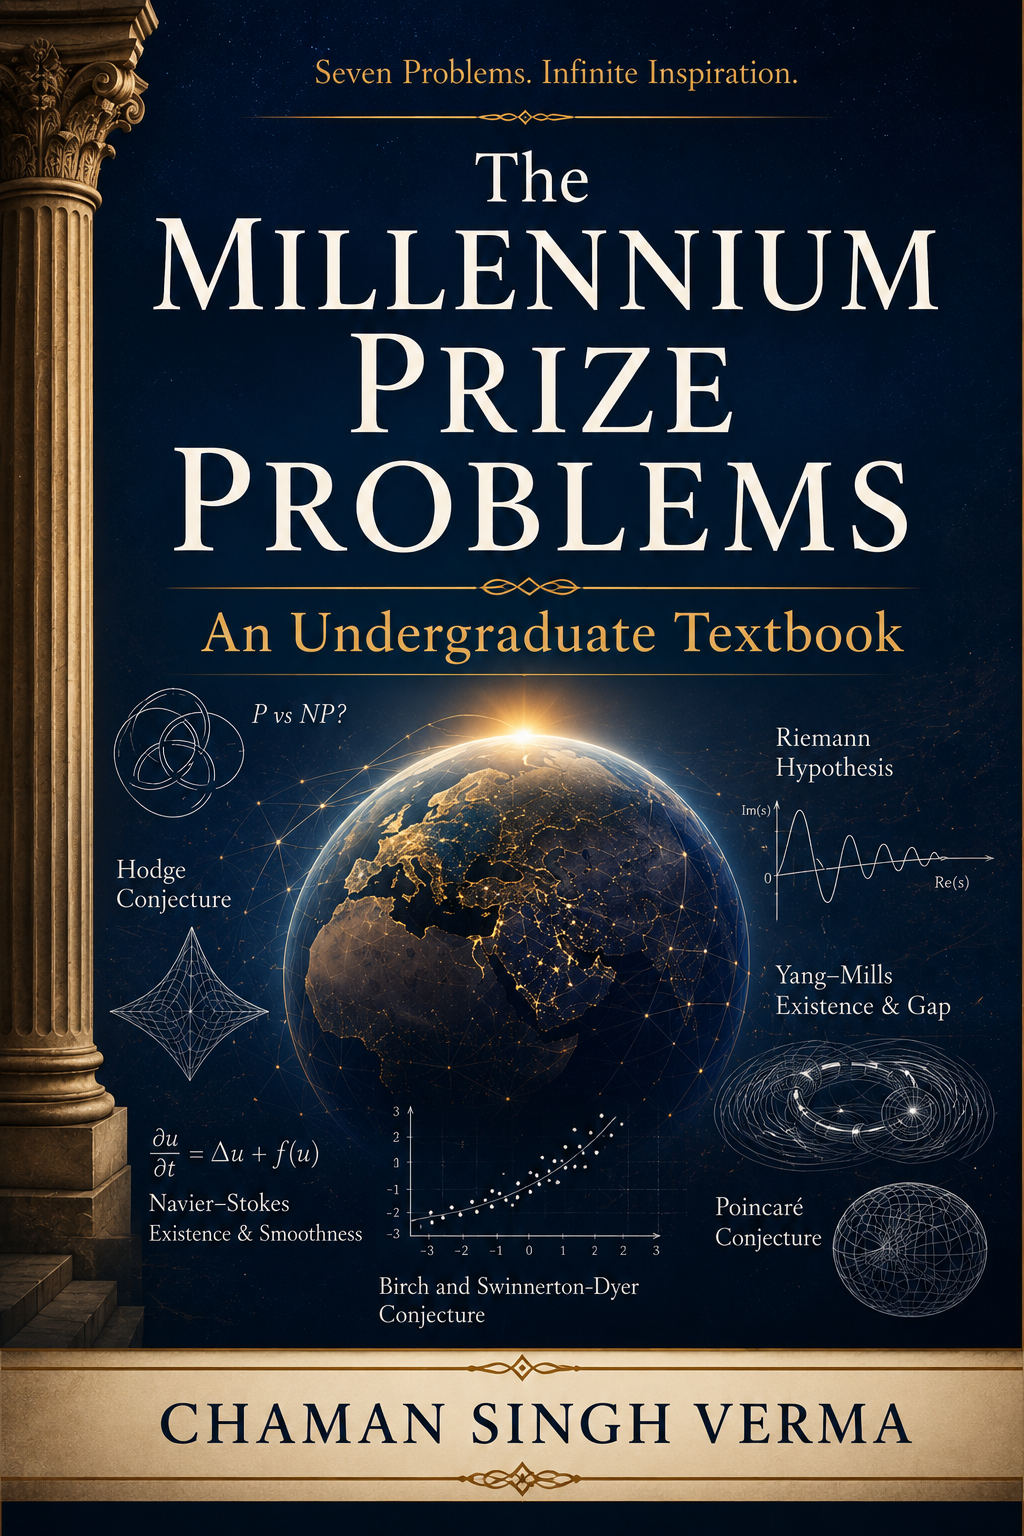
\includegraphics[width=\paperwidth,height=\paperheight,keepaspectratio]{frontpage.png}
\restoregeometry
\end{titlepage}

\tableofcontents
\listoffigures
\listoftables

\chapter*{Preface}
\addcontentsline{toc}{chapter}{Preface}

At the dawn of the twenty-first century, the Clay Mathematics Institute announced seven problems\footnote{See \url{https://www.claymath.org/millennium-problems}.} spanning the breadth of mathematics and theoretical physics. Each problem carries a prize of one million dollars. More importantly, each defines a frontier: a place where existing methods reach their limits and new ideas are needed. As of 2026, only one---the Poincar\'{e} conjecture---has been solved.

This book is an invitation to these frontiers. It is written for undergraduate students of mathematics, physics, computer science, and related fields who have completed a standard sequence in calculus, linear algebra, and basic abstract algebra. No graduate-level prerequisites are assumed, though some chapters draw on material (complex analysis, point-set topology, number theory) that may be encountered in advanced undergraduate courses. Each chapter is self-contained: the necessary concepts are developed from scratch, so readers need not work through the book in order.

\section*{The Seven Problems}

\begin{enumerate}
  \item \textbf{The Poincar\'{e} conjecture} (Chapter~\ref{ch:poincare}). Is every simply connected, closed three-manifold homeomorphic to the three-sphere? \textit{Solved} by Grigori Perelman in 2002--2003, building on Richard Hamilton's Ricci flow program.

  \item \textbf{The Riemann hypothesis} (Chapter~\ref{ch:riemann}). Do all non-trivial zeros of the Riemann zeta function lie on the critical line $\operatorname{Re}(s) = \tfrac{1}{2}$? The deepest open problem in number theory.

  \item \textbf{P vs NP} (Chapter~\ref{ch:pvsnp}). Does every problem whose solution can be \emph{verified} quickly also admit a solution that can be \emph{found} quickly? The central question of computational complexity.

  \item \textbf{The Navier--Stokes existence and smoothness problem} (Chapter~\ref{ch:navierstokes}). Do smooth, globally defined solutions to the incompressible Navier--Stokes equations exist in three dimensions for arbitrary smooth initial data? A problem at the intersection of analysis and fluid mechanics.

  \item \textbf{The Yang--Mills existence and mass gap} (Chapter~\ref{ch:yangmills}). Can quantum Yang--Mills theory be constructed rigorously, and does it exhibit a mass gap? A problem linking mathematics and quantum field theory.

  \item \textbf{The Hodge conjecture} (Chapter~\ref{ch:hodge}). Are certain cohomology classes on smooth projective complex varieties represented by algebraic cycles? A bridge between topology and algebraic geometry.

  \item \textbf{The Birch and Swinnerton-Dyer conjecture} (Chapter~\ref{ch:birch}). Does the rank of an elliptic curve over $\mathbb{Q}$ equal the order of vanishing of its $L$-function at $s = 1$? A central problem in arithmetic geometry.
\end{enumerate}

\section*{How to Use This Book}

Each chapter follows the same structure: a historical introduction, a development of the necessary mathematical background, a precise statement of the problem, a survey of known results and approaches, and a discussion of connections to other areas. Pedagogical features include:

\begin{itemize}
  \item \textbf{Key Ideas} (start of each chapter): A concise summary of the core concepts, so you know what to expect before diving in.
  \item \textbf{Worked Examples}: Detailed solutions to concrete problems, illustrating the techniques in action. Study these with pencil and paper before attempting the exercises.
  \item \textbf{Check Your Understanding}: Short questions placed after key definitions or results. Pause and try each one before reading on---they help you gauge whether you have absorbed the idea.
  \item \textbf{Exercises} (end of each chapter): Problems ranging from straightforward to challenging. The first few in each section require only an understanding of definitions; later ones develop new techniques and open doors to further study.
  \item \textbf{Chapter Summary} (end of each chapter): A recap of the main results, the key technique, and connections to other chapters.
\end{itemize}

We recommend the following approach:
\begin{enumerate}
  \item Read the introduction for motivation and historical context.
  \item Work through the technical sections, pausing at each ``Check Your Understanding.''
  \item Study the worked examples with pencil and paper.
  \item Attempt the exercises, starting with the easier ones.
  \item Read the chapter summary to consolidate what you have learned.
\end{enumerate}

\section*{Prerequisites by Chapter}

The chapters are not uniform in technical depth. Here is what each requires:

\begin{itemize}
  \item Chapter~\ref{ch:poincare} (Poincar\'{e}): multivariable calculus, basic topology
  \item Chapter~\ref{ch:riemann} (Riemann): complex analysis, elementary number theory
  \item Chapter~\ref{ch:pvsnp} (P vs NP): discrete mathematics, basic algorithms
  \item Chapter~\ref{ch:navierstokes} (Navier--Stokes): multivariable calculus, ODEs/PDEs
  \item Chapter~\ref{ch:yangmills} (Yang--Mills): linear algebra, basic physics
  \item Chapter~\ref{ch:hodge} (Hodge): linear algebra, basic algebraic geometry
  \item Chapter~\ref{ch:birch} (Birch--Swinnerton-Dyer): abstract algebra, elementary number theory
\end{itemize}

Chapters on the Riemann hypothesis and P vs NP are the most accessible. The chapters on Yang--Mills and Hodge require more background and may be better suited for a second course or an advanced reading seminar.

\section*{For Instructors}

This book is suitable for a one-semester topics course or a reading course. The seven chapters are independent and can be selected according to interest. Supplementary problem sets and lecture notes are available from the author.

\section*{Acknowledgments}

The author thanks the Clay Mathematics Institute for maintaining the official problem descriptions and for its support of the mathematical community. Special thanks to the many mathematicians whose work is summarized in these pages, and to the students who tested early versions of these chapters.

\mainmatter

%------------------------------------------------------------
% PART I: THE SOLVED PROBLEM
%------------------------------------------------------------
\part{The Solved Problem}

\chapter{The Poincar\'{e} Conjecture}
\label{ch:poincare}

\noindent\textbf{Key Ideas.}
\begin{itemize}
  \item A \emph{manifold}\index{manifold} is a space that locally looks like Euclidean space.
  \item The \emph{fundamental group}\index{fundamental group} detects holes by tracking how loops can be deformed.
  \item The Poincar\'{e} conjecture\index{Poincaré conjecture} asks: does trivial topology force a 3-manifold to be the 3-sphere?
  \item The proof uses the \emph{Ricci flow}\index{Ricci flow}---a PDE that evolves geometry to become uniform.
\end{itemize}

\bigskip

\section{Introduction}

The Poincar\'{e} conjecture is one of the most famous problems in mathematics. It is the only one of the seven Millennium Prize Problems to have been solved, and its solver---Grigori Perelman\index{Perelman}---turned down both the Fields Medal and the one-million-dollar prize.

In this chapter, we will develop the mathematical background needed to understand the conjecture, trace its history from Henri Poincar\'{e}'s original 1904 question to Perelman's 2002--2003 proof, and explore the human drama surrounding the solution. The story spans a century of mathematics, connecting topology, geometry, and analysis in unexpected ways.

The conjecture asks a deceptively simple question: \emph{if a three-dimensional space has no holes, must it be a three-sphere?} In two dimensions, the answer is yes: a closed surface without holes is a sphere. Poincar\'{e} asked whether this holds in three dimensions. The answer turned out to be yes, but proving it required a revolution in geometric analysis.

\begin{quote}
\textbf{Informal statement.} If you can stretch, bend, and deform a 3D shape without tearing it, and it has no ``holes''---must it be a sphere?
\end{quote}

The difficulty is that in three dimensions, our geometric intuition fails. There exist strange spaces that \emph{look} like $S^3$ from the perspective of loops and surfaces, but are not $S^3$. Detecting and ruling out these imposters is what makes the problem hard.

\section{Topological Preliminaries}

Before we can state the conjecture, we need to understand what a manifold is.

\begin{definition}
An \textit{$n$-dimensional topological manifold}\index{topological manifold} is a second-countable Hausdorff topological space $M$ such that every point has a neighborhood homeomorphic to $\mathbb{R}^n$ or the closed half-space $\mathbb{R}^n_{\ge 0} = \{(x_1, \ldots, x_n) : x_n \ge 0\}$.
\end{definition}

Points with a neighborhood homeomorphic to $\mathbb{R}^n_{\ge 0}$ but not to $\mathbb{R}^n$ form the \textit{boundary} $\partial M$. If $\partial M = \emptyset$, we say $M$ is a \textit{closed manifold} if it is also compact.

\begin{example}
The \textit{$n$-sphere}\index{sphere} $S^n = \{x \in \mathbb{R}^{n+1} : \|x\| = 1\}$ is a compact $n$-manifold without boundary.
\end{example}

\begin{example}
The \textit{$n$-torus}\index{torus} $T^n = S^1 \times \cdots \times S^1$ (product of $n$ circles) is a compact $n$-manifold.
\end{example}

\begin{example}
The \textit{real projective plane} $\mathbb{RP}^2$ is the set of lines through the origin in $\mathbb{R}^3$. It is a compact 2-manifold that cannot be embedded in $\mathbb{R}^3$ without self-intersection.
\end{example}

\begin{example}[A non-manifold]
A figure-eight is \emph{not} a manifold. At the crossing point, no neighborhood looks like $\mathbb{R}^1$---instead, four branches meet at a single point. Manifolds must look ``the same'' at every point, locally.
\end{example}

\begin{checkyou}
Which of the following are 2-manifolds? (a) A triangle (boundary of a 2-simplex), (b) a Möbius band\index{Möbius band}, (c) two circles joined at a point.
\end{checkyou}

\begin{definition}
Two spaces $X$ and $Y$ are \textit{homeomorphic}\index{homeomorphism} if there exists a continuous bijection $f: X \to Y$ with a continuous inverse. A homeomorphism preserves all topological properties.
\end{definition}

\begin{remark}
Two spaces are homeomorphic if one can be continuously deformed into the other without cutting or gluing. A coffee cup is homeomorphic to a doughnut. A sphere is \emph{not} homeomorphic to a torus.
\end{remark}

\begin{definition}
A space $X$ is \textit{contractible} if the identity map $\mathrm{id}_X$ is homotopic to a constant map.
\end{definition}

\begin{definition}
A space $X$ is \textit{simply connected}\index{simply connected} if it is path-connected and its fundamental group $\pi_1(X)$ is trivial.
\end{definition}

\begin{example}[The 2-sphere is simply connected]
\label{ex:s2simplyconnected}
We show that every loop on $S^2$ can be contracted to a point, proving $\pi_1(S^2) = 0$.

\textbf{Setup.} Let $\gamma: [0,1] \to S^2$ be an arbitrary loop based at $p \in S^2$, so $\gamma(0) = \gamma(1) = p$.

\textbf{Step 1: Reduce to a contractible case via stereographic projection.}
Since $S^2 \subset \mathbb{R}^3$, the image $\gamma([0,1])$ is a compact subset of $S^2$. By a dimension argument, $\gamma$ cannot be surjective: a continuous image of a 1-dimensional domain cannot cover a 2-dimensional manifold. Choose a point $q \in S^2$ not in the image of $\gamma$. The stereographic projection from $q$ is a homeomorphism:
\[
\sigma_q: S^2 \setminus \{q\} \;\xrightarrow{\;\sim\;}\; \mathbb{R}^2
\]
Since $\gamma$ never visits $q$, we may view $\gamma$ as a loop in $\mathbb{R}^2$.

\textbf{Step 2: Contract in $\mathbb{R}^2$.}
The space $\mathbb{R}^2$ is contractible. Define the straight-line homotopy $H: [0,1] \times [0,1] \to \mathbb{R}^2$ by:
\[
H(t, s) = (1 - s)\,\gamma(t) + s \cdot \sigma_q(p)
\]
At $s = 0$: $H(t,0) = \gamma(t)$ (the original loop). At $s = 1$: $H(t,1) = \sigma_q(p)$, a constant loop. For all $s$: $H(0,s) = H(1,s) = \sigma_q(p)$ (the basepoint is fixed). Each $H(\cdot, s)$ is continuous and its image lies in $\mathbb{R}^2$, which is convex, so $H$ is well-defined.

\textbf{Step 3: Transfer back to $S^2$.}
The map $\sigma_q^{-1}: \mathbb{R}^2 \to S^2 \setminus \{q\}$ is a homeomorphism. Define the homotopy on $S^2$:
\[
\widetilde{H}(t, s) = \sigma_q^{-1}\bigl(H(t, s)\bigr)
\]
This is a continuous deformation of $\gamma$ to the constant loop at $p$, lying entirely on $S^2$. Therefore $\gamma \simeq \mathrm{const}_p$, and since $\gamma$ was arbitrary, $\pi_1(S^2) = 0$. The 2-sphere is simply connected.
\end{example}

\subsection{The Fundamental Group}

In 1895, Henri Poincar\'{e}\index{Poincaré, Henri} introduced a powerful algebraic tool for studying manifolds: the fundamental group.

\begin{quote}
\textbf{Intuition.} Imagine the manifold is made of rubber. The fundamental group asks: which loops can be continuously shrunk to a point? If every loop can be shrunk, the space is simply connected (``no holes''). If some loops cannot be shrunk, the fundamental group records how they ``wrap around'' the holes.
\end{quote}

\begin{definition}
Let $X$ be a topological space with basepoint $x_0 \in X$. A \textit{loop} based at $x_0$ is a continuous map $\gamma: [0, 1] \to X$ with $\gamma(0) = \gamma(1) = x_0$. Two loops $\gamma_0, \gamma_1$ are \textit{homotopic} (written $\gamma_0 \simeq \gamma_1$) if there exists a continuous map $H: [0, 1] \times [0, 1] \to X$ such that $H(t, 0) = \gamma_0(t)$, $H(t, 1) = \gamma_1(t)$, and $H(0, s) = H(1, s) = x_0$ for all $t, s$.
\end{definition}

The set of homotopy classes of loops forms a group under concatenation:
\[
[\gamma_1] \cdot [\gamma_2] = [\gamma_1 \circ \gamma_2]
\]
where $\gamma_1 \circ \gamma_2$ means ``traverse $\gamma_1$ first, then $\gamma_2$.''

\begin{definition}
The \textit{fundamental group} $\pi_1(X, x_0)$ is the group of homotopy classes of loops based at $x_0$ with the concatenation operation.
\end{definition}

\begin{example}[$\pi_1(S^1) \cong \mathbb{Z}$ via the covering space $\mathbb{R} \to S^1$]
\label{ex:pi1s1}
We compute the fundamental group of the circle by lifting loops to its universal cover.

\textbf{The covering map.} Define $p: \mathbb{R} \to S^1$ by $p(t) = e^{2\pi i t} = (\cos 2\pi t,\, \sin 2\pi t)$. This is a covering map: every point of $S^1$ has an open neighborhood $U$ whose preimage $p^{-1}(U)$ is a disjoint union of open intervals in $\mathbb{R}$, each mapped homeomorphically onto $U$ by $p$.

\textbf{Step 1: Lifting loops.}
Let $\gamma: [0,1] \to S^1$ be a loop based at $1 \in S^1$, so $\gamma(0) = \gamma(1) = 1$. By the \textit{lifting property} of covering spaces, there exists a unique continuous lift $\tilde{\gamma}: [0,1] \to \mathbb{R}$ satisfying $p \circ \tilde{\gamma} = \gamma$ and $\tilde{\gamma}(0) = 0$.

Since $p(\tilde{\gamma}(1)) = \gamma(1) = 1 = p(0)$, we have $\tilde{\gamma}(1) \in p^{-1}(1) = \mathbb{Z}$. Define the \textit{winding number}:
\[
w(\gamma) = \tilde{\gamma}(1) \in \mathbb{Z}
\]
This is the integer that records how many times $\gamma$ winds around $S^1$.

\textbf{Step 2: Homotopic loops have the same winding number.}
Suppose $\gamma_0 \simeq \gamma_1$ via a homotopy $H: [0,1] \times [0,1] \to S^1$ fixing the basepoint. Lift $H$ to $\widetilde{H}: [0,1] \times [0,1] \to \mathbb{R}$ with $\widetilde{H}(t,0) = \tilde{\gamma}_0(t)$ and $\widetilde{H}(0,s) = 0$ for all $s$. Since $\widetilde{H}(1,s) \in \mathbb{Z}$ for each $s$ and $s \mapsto \widetilde{H}(1,s)$ is continuous, it must be constant (a continuous integer-valued function on a connected set is constant). Therefore $w(\gamma_0) = \widetilde{H}(1,0) = \widetilde{H}(1,1) = w(\gamma_1)$.

\textbf{Step 3: Every integer is realized.}
For any $k \in \mathbb{Z}$, the loop $\gamma_k(t) = e^{2\pi i k t}$ winds around $S^1$ exactly $k$ times. Its lift is $\tilde{\gamma}_k(t) = kt$, so $w(\gamma_k) = k$.

\textbf{Step 4: Winding number classifies loops up to homotopy.}
We must show that if $w(\gamma_0) = w(\gamma_1) = k$, then $\gamma_0 \simeq \gamma_1$. Since $w(\gamma_j) = k$, the lifts $\tilde{\gamma}_j$ both start at $0$ and end at $k$. Define:
\[
\widetilde{H}(t, s) = (1-s)\,\tilde{\gamma}_0(t) + s\,\tilde{\gamma}_1(t)
\]
This is a straight-line homotopy in $\mathbb{R}$ from $\tilde{\gamma}_0$ to $\tilde{\gamma}_1$. Since $\mathbb{R}$ is convex, $\widetilde{H}$ is continuous. Moreover, $\widetilde{H}(0,s) = 0$ and $\widetilde{H}(1,s) = k$ for all $s$, so the basepoint is fixed. Projecting down: $H = p \circ \widetilde{H}$ is a homotopy in $S^1$ from $\gamma_0$ to $\gamma_1$.

\textbf{Conclusion.} The map $w: \pi_1(S^1) \to \mathbb{Z}$ is a well-defined, surjective bijection. It is a group homomorphism (winding numbers add under loop concatenation), hence an isomorphism: $\pi_1(S^1) \cong \mathbb{Z}$.
\end{example}

For path-connected spaces, $\pi_1(X, x_0) \cong \pi_1(X, x_1)$ for any two basepoints, so we often write $\pi_1(X)$.

\begin{example}
$\pi_1(S^n) = 0$ for $n \ge 2$. On the $2$-sphere, any loop can be contracted to a point. Think of a rubber band on a basketball: you can always slide it off.
\end{example}

\begin{example}
$\pi_1(S^1) \cong \mathbb{Z}$. The nontrivial loops wrap around the circle $k$ times. This is why a rubber band around a cylinder cannot be contracted---it wraps around the hole.
\end{example}

\begin{example}
$\pi_1(T^2) \cong \mathbb{Z} \times \mathbb{Z}$, generated by loops around each independent circle direction.
\end{example}

\begin{example}
$\pi_1(\mathbb{R}^n) = 0$ for all $n$, since $\mathbb{R}^n$ is contractible---any loop can be pulled to a point.
\end{example}

\begin{checkyou}
Why is the fundamental group of a figure-eight (two circles joined at a point) the free group on two generators, while the fundamental group of a circle is $\mathbb{Z}$?
\end{checkyou}

\begin{definition}
A space $X$ is \textit{simply connected} if it is path-connected and $\pi_1(X)$ is the trivial group.
\end{definition}

\begin{checkyou}
Is $\mathbb{R}^n$ simply connected? What about $\mathbb{R}^n \setminus \{0\}$? Why or why not?
\end{checkyou}

\subsection{Higher Homotopy Groups}

The fundamental group is only the first in a sequence of homotopy groups $\pi_n(X)$ for $n \ge 1$. The $n$-th homotopy group consists of homotopy classes of maps $S^n \to X$. A theorem of Hurewicz relates homotopy groups to homology groups, which are often easier to compute.

\begin{theorem}[Hurewicz Theorem]
If $X$ is simply connected, then the first nontrivial homotopy group $\pi_n(X)$ is isomorphic to the first nontrivial homology group $H_n(X)$.
\end{theorem}

\subsection{Homology and Cohomology}

While homotopy groups capture information about maps from spheres, homology groups capture information about cycles and boundaries in a space.

\begin{definition}
For a topological space $X$, the \textit{singular homology groups} $H_n(X; \mathbb{Z})$ are abelian groups that count $n$-dimensional ``holes'' in $X$. The $n$-th Betti number\index{Betti numbers} is $b_n = \mathrm{rank}(H_n(X; \mathbb{Z}))$.
\end{definition}

\begin{example}
For $S^n$: $H_0(S^n) = \mathbb{Z}$, $H_n(S^n) = \mathbb{Z}$, and $H_k(S^n) = 0$ for $0 < k < n$.
\end{example}

\begin{example}
For $T^n$: $H_k(T^n) = \mathbb{Z}^{\binom{n}{k}}$.
\end{example}

\subsection{The Classification of Surfaces}

Before attacking three-dimensional manifolds, mathematicians classified all compact 2-manifolds (surfaces)\index{surface}. The theorem is elegant:

\begin{theorem}[Classification of compact surfaces]
Every closed, connected, orientable 2-manifold\index{orientable} is homeomorphic to a sphere with $g$ handles ($g \ge 0$), called the \textit{genus-$g$ surface} $\Sigma_g$. The number $g$ is called the \textit{genus}\index{genus}. Non-orientable surfaces are homeomorphic to connected sums of $\mathbb{RP}^2$'s.
\end{theorem}

In particular, a simply connected closed surface must be the 2-sphere $S^2$. This is the 2-dimensional analogue of the Poincar\'{e} conjecture.

\begin{figure}[htbp]
\centering
\begin{tikzpicture}[scale=0.9]
  % Sphere (genus 0)
  \begin{scope}[xshift=-3.5cm]
    \draw[thick] (0,0) circle (1.2);
    \draw[thick,dashed] (-1.2,0) arc[start angle=180, end angle=360, x radius=1.2, y radius=0.4];
    \node at (0,-1.8) {\small Sphere};
    \node at (0,-2.2) {\small genus $g=0$};
  \end{scope}
  % Torus (genus 1)
  \begin{scope}[xshift=0cm]
    \draw[thick] (-1.2,-0.8) arc[start angle=180, end angle=360, x radius=1.2, y radius=0.8];
    \draw[thick] (-1.2,0.8) arc[start angle=180, end angle=360, x radius=1.2, y radius=0.8];
    \draw[thick] (-1.2,-0.8) -- (-1.2,0.8);
    \draw[thick] (1.2,-0.8) -- (1.2,0.8);
    \draw[thick,dashed] (0,0) ellipse[x radius=0.5, y radius=0.45];
    \node at (0,-1.6) {\small Torus};
    \node at (0,-2.0) {\small genus $g=1$};
  \end{scope}
  % Genus-2 surface
  \begin{scope}[xshift=4cm]
    \draw[thick] (-1.5,0) .. controls (-1.5,1.0) and (-0.3,1.0) .. (-0.3,0);
    \draw[thick] (-0.3,0) .. controls (-0.3,-1.0) and (-1.5,-1.0) .. (-1.5,0);
    \draw[thick] (0.3,0) .. controls (0.3,1.0) and (1.5,1.0) .. (1.5,0);
    \draw[thick] (1.5,0) .. controls (1.5,-1.0) and (0.3,-1.0) .. (0.3,0);
    \draw[thick] (-0.3,0.5) .. controls (-0.1,0.6) and (0.1,0.6) .. (0.3,0.5);
    \draw[thick] (-0.3,-0.5) .. controls (-0.1,-0.6) and (0.1,-0.6) .. (0.3,-0.5);
    \node at (0,-1.6) {\small Double torus};
    \node at (0,-2.0) {\small genus $g=2$};
  \end{scope}
\end{tikzpicture}
\caption{The classification of surfaces by genus: every closed orientable surface is homeomorphic to a sphere with $g$ handles.}
\label{fig:surfaces}
\end{figure}

\subsection{Connected Sum and Prime Decomposition}

For 3-manifolds, there is an analogous operation to the connected sum of surfaces.

\begin{definition}
The \textit{connected sum} $M \# N$ of two $n$-manifolds is formed by removing an $n$-ball from each and gluing the resulting boundaries.
\end{definition}

\begin{theorem}[Prime decomposition, Kneser 1929; uniqueness, Milnor 1962]
Every closed, orientable 3-manifold can be uniquely decomposed as a connected sum of \textit{prime} 3-manifolds (manifolds that cannot be written as a nontrivial connected sum).
\end{theorem}

The Poincar\'{e} conjecture is equivalent to: every simply connected prime 3-manifold is $S^3$.

\section{Statement of the Conjecture}

The Poincar\'{e} conjecture asks whether the analogous statement holds in three dimensions:

\begin{theorem}[Poincar\'{e} conjecture, now proved]
Every simply connected, closed 3-manifold is homeomorphic to the 3-sphere\index{three-sphere} $S^3$.
\end{theorem}

\begin{remark}
The 3-sphere is the set $\{(x_1, x_2, x_3, x_4) \in \mathbb{R}^4 : x_1^2 + x_2^2 + x_3^2 + x_4^2 = 1\}$. It is the natural generalization of an ordinary sphere to one dimension higher.
\end{remark}

\begin{figure}[htbp]
\centering
\begin{tikzpicture}[scale=0.7]
  % Step 1: loop on sphere
  \begin{scope}[xshift=-5.5cm]
    \draw[thick] (0,0) circle (1.2);
    \draw[thick,dashed] (-1.2,0) arc[start angle=180, end angle=360, x radius=1.2, y radius=0.4];
    \draw[blue,very thick] (0.5,0.9) .. controls (1.0,0.5) and (1.0,-0.5) .. (0.5,-0.9)
      .. controls (0.0,-0.5) and (0.0,0.5) .. (0.5,0.9);
    \fill (0.5,0.9) circle (2pt) node[above right] {\small $p$};
  \end{scope}
  % Step 2: loop shrinking
  \begin{scope}[xshift=-1.8cm]
    \draw[thick] (0,0) circle (1.2);
    \draw[thick,dashed] (-1.2,0) arc[start angle=180, end angle=360, x radius=1.2, y radius=0.4];
    \draw[blue,very thick,opacity=0.5] (0.5,0.9) .. controls (1.0,0.5) and (1.0,-0.5) .. (0.5,-0.9)
      .. controls (0.0,-0.5) and (0.0,0.5) .. (0.5,0.9);
    \draw[blue,very thick] (0.3,0.5) .. controls (0.6,0.3) and (0.6,-0.3) .. (0.3,-0.5)
      .. controls (0.0,-0.2) and (0.0,0.2) .. (0.3,0.5);
    \fill (0.3,0.5) circle (2pt) node[above right] {\small $p$};
  \end{scope}
  % Step 3: loop almost a point
  \begin{scope}[xshift=1.8cm]
    \draw[thick] (0,0) circle (1.2);
    \draw[thick,dashed] (-1.2,0) arc[start angle=180, end angle=360, x radius=1.2, y radius=0.4];
    \draw[blue,very thick] (0.15,0.15) circle (0.15);
    \fill (0.15,0.15) circle (2pt) node[above right] {\small $p$};
  \end{scope}
  % Step 4: contracted to point
  \begin{scope}[xshift=5.5cm]
    \draw[thick] (0,0) circle (1.2);
    \draw[thick,dashed] (-1.2,0) arc[start angle=180, end angle=360, x radius=1.2, y radius=0.4];
    \fill (0,0) circle (2pt) node[above right] {\small $p$};
  \end{scope}
  % Labels below each sphere
  \node at (-5.5,-1.8) {\small Step 1};
  \node at (-1.8,-1.8) {\small Step 2};
  \node at (1.8,-1.8) {\small Step 3};
  \node at (5.5,-1.8) {\small Step 4};
  % Arrows between steps
  \draw[->,thick,gray] (-4.0,-1.8) -- (-3.3,-1.8);
  \draw[->,thick,gray] (-0.3,-1.8) -- (0.4,-1.8);
  \draw[->,thick,gray] (3.3,-1.8) -- (4.0,-1.8);
\end{tikzpicture}
\caption{Any loop on a simply connected surface (such as $S^2$) can be continuously contracted to a point. This is the property that the Poincar\'{e} conjecture seeks to generalize to three dimensions.}
\label{fig:loop_contraction}
\end{figure}

\begin{remark}
The analogue holds in all dimensions $\ge 5$ (proved by Stephen Smale in 1961, Fields Medal 1966) and in dimension 4 (proved by Michael Freedman in 1982, Fields Medal 1986). Dimension 3 was the hardest case.
\end{remark}

\subsection{The Poincar\'{e} Conjecture in Higher Dimensions}

It is worth understanding why dimensions $\ge 5$ were easier. The key technique is the \textit{h-cobordism theorem} and \textit{surgery theory}\index{surgery theory}.

\begin{theorem}[Smale's h-cobordism theorem]
Let $W$ be a compact $(n+1)$-manifold with boundary $\partial W = M_0 \cup M_1$, where $M_0$ and $M_1$ are $n$-manifolds. If $n \ge 5$ and $W$, $M_0$, $M_1$ are simply connected, and the inclusion $M_0 \hookrightarrow W$ is a homotopy equivalence\index{homotopy equivalence}, then $W$ is diffeomorphic to $M_0 \times [0,1]$.
\end{theorem}

This theorem allows one to build a cobordism between a homotopy sphere and the standard sphere, and then conclude they are diffeomorphic. The proof requires the \textit{Whitney trick} to eliminate intersections of disks, which works in dimensions $\ge 5$ but fails in dimensions 3 and 4.

In dimension 4, Freedman's proof used topological (not smooth) methods and the \textit{Casson handle} construction, which is an infinite tower of disks that substitutes for the Whitney trick.

\subsection{Historical Formulations}

Poincar\'{e} originally stated the conjecture in 1904 in the fifth supplement to his \textit{Analysis Situs}:

\begin{quote}
``Une question se pose: Est-il possible que le groupe fondamental d'une vari\'{e}t\'{e} de trois dimensions soit r\'{e}duit \`{a} l'identit\'{e} sans que cette vari\'{e}t\'{e} soit simplement connexe? ... Je ne suis pas parvenu \`{a} r\'{e}soudre cette question.''
\end{quote}

(A question arises: Is it possible that the fundamental group of a 3-dimensional manifold could be reduced to the identity without the manifold being simply connected? ... I have not succeeded in solving this question.)

He later modified the question to ask whether every closed 3-manifold with trivial fundamental group is homeomorphic to $S^3$. The conjecture in its modern form was thus established.

\section{Hamilton's Program: The Ricci Flow}

The key to proving the Poincar\'{e} conjecture was the \textit{Ricci flow}, introduced by Richard Hamilton\index{Hamilton} in 1982.

\begin{quote}
\textbf{Intuition.} The Ricci flow is the ``heat equation for geometry.'' Just as heat spreads out from hot spots to make temperature uniform, the Ricci flow smooths out the curvature of a manifold to make it round. If you start with any 3-manifold and flow, the geometry should eventually look like a sphere.
\end{quote}

\begin{definition}
Let $(M, g)$ be a Riemannian manifold with metric $g_{ij}$. The \textit{Ricci flow} is the evolution equation:
\[
\frac{\partial}{\partial t} g_{ij} = -2 R_{ij}
\]
where $R_{ij}$ is the Ricci curvature tensor.
\end{definition}

\begin{checkyou}
In what sense is the Ricci flow like the heat equation? What plays the role of ``temperature''?
\end{checkyou}

The Ricci curvature $R_{ij}$ measures how the volume of a small ball deviates from Euclidean volume. Regions of positive Ricci curvature shrink under the flow; regions of negative Ricci curvature expand.

Think of the Ricci flow as the geometric analogue of the heat equation. Just as heat diffuses from hot regions to cold regions, the Ricci flow smooths out irregularities in the metric, making the geometry more uniform over time.

\subsection{The Heat Analogy}

The ordinary heat equation $\partial_t u = \Delta u$ describes how temperature diffuses. A hot object eventually reaches uniform temperature. Similarly, under the Ricci flow, a manifold with positive Ricci curvature should evolve toward a round sphere---the 3-sphere.

Hamilton showed that in dimension 2, the Ricci flow does indeed deform any metric on a closed surface to a constant-curvature metric, providing a new proof of the uniformization theorem. He also showed that in dimension 3, if the Ricci flow can be continued indefinitely without developing singularities, it would prove the Poincar\'{e} conjecture.

\begin{figure}[htbp]
\centering
\begin{tikzpicture}[scale=0.75]
  % Dumbbell shape evolving under Ricci flow (Hamilton's picture)
  % Stage 1: pinched dumbbell
  \begin{scope}[xshift=-5.5cm]
    \draw[thick] (-0.8,0.7) .. controls (-0.8,1.2) and (0.8,1.2) .. (0.8,0.7)
      .. controls (0.3,0.5) and (0.3,0.3) .. (0.8,0.1)
      .. controls (0.3,-0.1) and (0.3,-0.3) .. (0.8,-0.5)
      .. controls (0.8,-1.2) and (-0.8,-1.2) .. (-0.8,-0.5)
      .. controls (-0.3,-0.3) and (-0.3,-0.1) .. (-0.8,0.1)
      .. controls (-0.3,0.3) and (-0.3,0.5) .. (-0.8,0.7);
    \node at (0,-1.7) {\small $t=0$};
  \end{scope}
  % Stage 2: slightly less pinched
  \begin{scope}[xshift=-1.8cm]
    \draw[thick] (-0.8,0.75) .. controls (-0.8,1.15) and (0.8,1.15) .. (0.8,0.75)
      .. controls (0.2,0.55) and (0.2,0.45) .. (0.8,0.15)
      .. controls (0.2,-0.05) and (0.2,-0.15) .. (0.8,-0.55)
      .. controls (0.8,-1.15) and (-0.8,-1.15) .. (-0.8,-0.55)
      .. controls (-0.2,-0.15) and (-0.2,-0.05) .. (-0.8,0.15)
      .. controls (-0.2,0.45) and (-0.2,0.55) .. (-0.8,0.75);
    \node at (0,-1.7) {\small $t=t_1$};
  \end{scope}
  % Stage 3: rounding out
  \begin{scope}[xshift=1.9cm]
    \draw[thick] (-0.7,0.6) .. controls (-0.7,1.0) and (0.7,1.0) .. (0.7,0.6)
      .. controls (0.15,0.45) and (0.15,0.35) .. (0.7,0.1)
      .. controls (0.15,-0.1) and (0.15,-0.2) .. (0.7,-0.5)
      .. controls (0.7,-1.0) and (-0.7,-1.0) .. (-0.7,-0.5)
      .. controls (-0.15,-0.2) and (-0.15,-0.1) .. (-0.7,0.1)
      .. controls (-0.15,0.35) and (-0.15,0.45) .. (-0.7,0.6);
    \node at (0,-1.7) {\small $t=t_2$};
  \end{scope}
  % Stage 4: nearly round
  \begin{scope}[xshift=5.6cm]
    \draw[thick] (0,0) circle (0.95);
    \draw[thick,dashed] (-0.95,0) arc[start angle=180, end angle=360, x radius=0.95, y radius=0.35];
    \node at (0,-1.7) {\small $t \to \infty$};
  \end{scope}
  % Arrows
  \draw[->,thick] (-3.7,0) -- (-3.0,0);
  \draw[->,thick] (0.1,0) -- (0.8,0);
  \draw[->,thick] (3.7,0) -- (4.4,0);
\end{tikzpicture}
\caption{The Ricci flow smooths out irregularities in curvature, analogous to heat diffusion. A ``dumbbell'' shape with a thin neck (high curvature) evolves toward a round sphere. The thin neck pinches off and the geometry becomes uniform.}
\label{fig:ricci_flow_dumbbell}
\end{figure}

\subsection{The Singularity Problem}

The obstacle that stymied Hamilton was the formation of \textit{singularities}. As the flow evolves a 3-manifold, regions of extreme curvature can develop, causing the flow to break down. Imagine a rubber band being stretched until it snaps---that is analogous to a singularity.

Hamilton identified several possible singularity types and developed a program for handling them:
\begin{enumerate}
  \item Understand the possible singularity models
  \item Show that certain bad singularities do not occur
  \item When singularities occur, perform ``surgery'' to remove them
  \item Show that after finitely many surgeries, the manifold decomposes into pieces with uniform geometry
\end{enumerate}

He was unable to complete steps 1--3.

\subsection{Hamilton's Results}

Hamilton made remarkable progress:
\begin{itemize}
  \item Short-time existence and uniqueness for Ricci flow on compact manifolds
  \item In dimension 2: Ricci flow converges to constant curvature metric (uniformization)
  \item In dimension 3: if initial metric has positive Ricci curvature, the flow exists for all time and converges to round sphere
  \item Development of the maximum principle for systems of PDEs on manifolds
  \item Introduction of the differential Harnack inequality for Ricci flow
\end{itemize}

But the general case with arbitrary initial metrics remained out of reach.

\section{Perelman's Breakthrough}

Grigori Perelman, working alone in Saint Petersburg, made three key contributions that completed Hamilton's program.

\subsection{1. The Entropy Functional}

In his first paper (November 2002), Perelman introduced the $\mathcal{F}$ and $\mathcal{W}$ functionals. The $\mathcal{W}$ functional, which he called the \textit{entropy}\index{entropy}, is:

\[
\mathcal{W}(g, f, \tau) = \int_M \bigl[\tau(|\nabla f|^2 + R) + f - n\bigr] (4\pi\tau)^{-n/2} e^{-f} \, dV
\]

where $f$ is a smooth function on $M$ and $\tau > 0$ is a parameter.

\begin{theorem}[Perelman, 2002]
The $\mathcal{W}$ functional is monotone non-decreasing under the Ricci flow coupled with a certain evolution equation for $f$. Moreover, $\mathcal{W}$ is bounded below.
\end{theorem}

This monotonicity gave Perelman unprecedented control over the formation of singularities. He used it to show that singularities must be of a very specific type: they must be \textit{asymptotically cylindrical} or \textit{asymptotically paraboloidal}. In particular, singularities cannot accumulate.

\subsection{2. No Local Collapsing Theorem}

A second crucial result: Perelman showed that the Ricci flow cannot develop a singularity where the geometry collapses to arbitrarily small scales---he called this \textit{no local collapsing}. This ruled out certain pathological singularity types that Hamilton could not exclude.

\begin{theorem}[Perelman, No Local Collapsing]
Under the Ricci flow on a closed 3-manifold, there is no sequence of points and scales where the injectivity radius tends to zero while the curvature remains bounded.
\end{theorem}

The proof uses the $\mathcal{W}$ entropy and a clever scaling argument.

\subsection{3. Ricci Flow with Surgery}

In his second paper (March 2003), Perelman described an explicit surgical procedure. When a singularity begins to form (the curvature becomes large in a small region), he showed how to cut out the singular region and replace it with a smooth cap. The surgery can be performed at a precise curvature threshold, and the procedure can be repeated.

\begin{theorem}[Perelman, 2003]
For any initial metric on a closed 3-manifold, the Ricci flow with surgery can be continued for all time, with only finitely many surgeries occurring.
\end{theorem}

The third paper (July 2003) proved that after finitely many surgeries, all remaining components are diffeomorphic to spherical space forms or $S^2 \times S^1$, and for a simply connected manifold, only a single $S^3$ remains.

\subsection{The Canonical Neighborhood Theorem}

A key technical result in Perelman's work is the \textit{canonical neighborhood theorem}, which classifies the geometry of high-curvature regions. Every point of sufficiently high curvature has a neighborhood that is, after rescaling, close to one of a few model geometries:
\begin{itemize}
  \item A neck region (approximately $S^2 \times \mathbb{R}$)
  \item A cap region (approximately a capped cylinder)
  \item A component that is globally close to a spherical space form
\end{itemize}

This classification makes surgery possible: one cuts along the necks and caps the ends.

\subsection{Finite Extinction Time}

Perelman also proved that for any initial metric on a simply connected 3-manifold, the Ricci flow with surgery becomes extinct in finite time---meaning the manifold disappears entirely, having been completely decomposed into spherical space forms. This is a stronger result than just proving the Poincar\'{e} conjecture.

\begin{checkyou}
Why does finite extinction time imply the Poincar\'{e} conjecture for simply connected manifolds?
\end{checkyou}

\section{Verification and Acceptance}

Perelman posted his papers on the arXiv preprint server rather than submitting them to journals. The mathematical community faced the challenge of verifying his work:

\begin{itemize}
  \item \textbf{2003:} Perelman visited the US to lecture at MIT, Princeton, Stony Brook, and Columbia.
  \item \textbf{2003--2006:} Bruce Kleiner and John Lott wrote detailed notes.
  \item \textbf{2004--2006:} John Morgan and Gang Tian wrote a comprehensive exposition.
  \item \textbf{2006:} The International Mathematical Union awarded Perelman the Fields Medal.
  \item \textbf{2010:} The Clay Mathematics Institute awarded the Millennium Prize.
\end{itemize}

Perelman declined both awards. He told a journalist: ``I'm not interested in money or fame. I don't want to be on display like an animal in a zoo.''

\subsection{The Verification Efforts}

Three major teams worked on verifying Perelman's proof:
\begin{enumerate}
  \item \textbf{Kleiner--Lott:} Detailed notes on all three papers, published in \textit{Geometry \& Topology} (2008).
  \item \textbf{Morgan--Tian:} Book-length exposition \textit{Ricci Flow and the Poincar\'{e} Conjecture} (AMS, 2007).
  \item \textbf{Cao--Zhu:} Published in \textit{Asian Journal of Mathematics} (2006), though later controversy arose about attribution.
\end{enumerate}

All three teams confirmed the correctness of Perelman's arguments. The mathematical community reached consensus that the Poincar\'{e} conjecture was proved.

\section{The Thurston Geometrization Conjecture}

Perelman's proof actually accomplished far more than the Poincar\'{e} conjecture. He proved the \textit{Thurston geometrization conjecture}\index{Thurston's geometrization}, which classifies \textit{all} 3-manifolds.

\begin{theorem}[Thurston geometrization, proved by Perelman]
Every closed 3-manifold can be decomposed along spheres and tori into pieces that admit one of eight geometric structures (the eight Thurston geometries): $S^3$, $\mathbb{E}^3$, $\mathbb{H}^3$, $S^2 \times \mathbb{R}$, $\mathbb{H}^2 \times \mathbb{R}$, $\widetilde{SL_2(\mathbb{R})}$, $\mathrm{Nil}$, and $\mathrm{Sol}$.
\end{theorem}

This is analogous to the classification of surfaces, but vastly richer and more complex.

\subsection{The Eight Thurston Geometries}

The eight model geometries for 3-manifolds are:
\begin{enumerate}
  \item \textbf{Spherical ($S^3$):} Positive constant curvature. Compact.
  \item \textbf{Euclidean ($\mathbb{E}^3$):} Zero curvature. Flat.
  \item \textbf{Hyperbolic ($\mathbb{H}^3$):} Negative constant curvature. Most 3-manifolds are hyperbolic.
  \item \textbf{$S^2 \times \mathbb{R}$:} Product of sphere and line.
  \item \textbf{$\mathbb{H}^2 \times \mathbb{R}$:} Product of hyperbolic plane and line.
  \item \textbf{$\widetilde{SL_2(\mathbb{R})}$}: Universal cover of the unit tangent bundle of $\mathbb{H}^2$.
  \item \textbf{Nil}: Nilpotent Lie group (Heisenberg group).
  \item \textbf{Sol}: Solvable Lie group.
\end{enumerate}

Every closed 3-manifold admits a unique decomposition (the \textit{geometric decomposition}) into pieces that have one of these geometries.

\subsection{The Poincar\'{e} Conjecture as a Special Case}

The Poincar\'{e} conjecture follows immediately: a simply connected closed 3-manifold must be a spherical space form. The only simply connected spherical space form is $S^3$ itself.

\section{The Human Story}

The solution of the Poincar\'{e} conjecture involves one of the most remarkable human stories in modern mathematics.

\subsection{Grigori Perelman}

Grigori Perelman (born 1966) was a child prodigy in Leningrad. He won a gold medal with a perfect score at the 1982 International Mathematical Olympiad. He received his Ph.D. from Leningrad State University under the direction of Aleksandr Aleksandrov. He worked at the Steklov Institute in Saint Petersburg.

In 1992--1993, Perelman spent time in the US at NYU, SUNY Stony Brook, and UC Berkeley. Colleagues remember him as intensely focused, living ascetically, and completely dedicated to mathematics. He returned to Saint Petersburg and worked in isolation for seven years before posting his papers.

\subsection{The Controversies}

The verification process was not without controversy:
\begin{itemize}
  \item The Cao--Zhu paper initially claimed credit for ``completing'' Perelman's work, leading to protests from the mathematical community.
  \item Perelman was offered the Fields Medal in 2006 at the International Congress of Mathematicians in Madrid. He declined, and did not attend.
  \item The Clay Institute awarded the Millennium Prize in 2010. Perelman declined the prize money, saying his contribution was no greater than Hamilton's.
  \item Perelman resigned from the Steklov Institute in 2005 and has reportedly not done mathematics since.
\end{itemize}

\subsection{Richard Hamilton}

Richard Hamilton (born 1943) developed the Ricci flow program over two decades. He proved the foundational results and guided the program to the point where Perelman could complete it. Hamilton received the Shaw Prize in 2011 and the AMS Steele Prize in 2009. He has been gracious in acknowledging Perelman's achievement.

\subsection{William Thurston}

William Thurston (1946--2012) formulated the geometrization conjecture in the 1970s. His visionary insight was that 3-manifolds should be understood through geometry. He received the Fields Medal in 1982. Perelman's proof realized Thurston's vision.

\section{The Ricci Flow in Higher Dimensions}

The Ricci flow has been extensively studied in higher dimensions since Perelman's work.

\begin{itemize}
  \item \textbf{Dimension 4:} The Ricci flow with surgery is more complicated due to the presence of \textit{orbifold} singularities and the lack of a canonical neighborhood theorem as clean as in dimension 3. Recent work by Bamler, Kleiner, and others has made progress.
  \item \textbf{K\"{a}hler-Ricci flow:} On K\"{a}hler manifolds, the Ricci flow preserves the K\"{a}hler condition. This has applications to the classification of algebraic varieties (the Minimal Model Program).
  \item \textbf{Ancient solutions:} Classification of ancient solutions (solutions existing for all negative time) is a major area of study.
\end{itemize}

\section{Applications and Legacy}

The resolution of the Poincar\'{e} conjecture has had far-reaching consequences:

\subsection{Geometric Topology}
\begin{itemize}
  \item Complete classification of 3-manifolds (geometrization)
  \item Solution to the homeomorphism problem for 3-manifolds
  \item Understanding of the mapping class groups of 3-manifolds
\end{itemize}

\subsection{Geometric Analysis}
\begin{itemize}
  \item New techniques for nonlinear PDE on manifolds (entropy, pseudolocality, surgery)
  \item Development of the theory of Ricci flow as a field in its own right
  \item Applications to the differentiable sphere theorem (Brendle-Schoen, 2008)
\end{itemize}

\subsection{Physics}
\begin{itemize}
  \item Ricci flow as renormalization group flow in string theory
  \item Connections to the AdS/CFT correspondence
  \item Understanding of topology change in quantum gravity
\end{itemize}

\section{Exercises}

\begin{exercise}
Show that $S^2$ is simply connected by constructing an explicit homotopy contracting any loop to a point.
\end{exercise}

\begin{exercise}
Compute $\pi_1(\mathbb{R}^2 \setminus \{0\})$.
\end{exercise}

\begin{exercise}
Show that the fundamental group of the figure-eight space (two circles joined at a point) is the free group on two generators.
\end{exercise}

\begin{exercise}
Explain in your own words why the Ricci flow analogy with the heat equation is useful. What are the key differences?
\end{exercise}

\begin{exercise}
Research the proof of the 2-dimensional analogue: why is every simply connected closed surface homeomorphic to $S^2$?
\end{exercise}

\begin{exercise}
The Poincar\'{e} conjecture in dimension 5 and higher was proved by Smale using surgery theory. Write a one-page summary of how surgery works.
\end{exercise}

\begin{exercise}
\textbf{Challenge problem.} A \textit{Hopf fibration} is a map $h: S^3 \to S^2$ whose fibers are circles. Show that $S^3$ can be described as the union of two solid tori glued along their boundaries. Use this to compute $\pi_1(S^3)$.
\end{exercise}

\begin{exercise}
Let $M$ be a closed 3-manifold with $\pi_1(M) = 0$. Show that $H_1(M; \mathbb{Z}) = 0$ and $H_2(M; \mathbb{Z}) = 0$. (Hint: use the Hurewicz theorem and Poincar\'{e} duality.)
\end{exercise}

\begin{exercise}
Explain the difference between a topological manifold, a smooth manifold, and a PL (piecewise-linear) manifold. Why did the Poincar\'{e} conjecture hold in all three categories in dimension 3?
\end{exercise}

\begin{exercise}
The \textit{Poincar\'{e} homology sphere} is a 3-manifold with the same homology as $S^3$ but with fundamental group of order 120. Describe its construction as a quotient of $S^3$ by a finite group action.
\end{exercise}

\section{Further Reading}

\begin{itemize}
  \item J. Milnor, ``The Poincar\'{e} conjecture,'' official Clay problem description
  \item J. Morgan and G. Tian, \textit{Ricci Flow and the Poincar\'{e} Conjecture}, AMS, 2007
  \item A. Hatcher, \textit{Algebraic Topology}, Cambridge, 2002
  \item B. Kleiner and J. Lott, ``Notes on Perelman's papers,'' \textit{Geometry \& Topology}, 2008
  \item H.-D. Cao and X.-P. Zhu, ``A complete proof of the Poincar\'{e} and geometrization conjectures,'' \textit{Asian J. Math.}, 2006
  \item J. W. Morgan, ``Recent progress on the Poincar\'{e} conjecture and the classification of 3-manifolds,'' \textit{Bull. AMS}, 2005
  \item D. Anderson, ``The Poincar\'{e} conjecture,'' \textit{Notices AMS}, 2004
  \item G. Perelman, ``The entropy formula for the Ricci flow and its geometric applications,'' arXiv:math/0211159
  \item G. Perelman, ``Ricci flow with surgery on three-manifolds,'' arXiv:math/0303109
  \item G. Perelman, ``Finite extinction time for the solutions to the Ricci flow on certain three-manifolds,'' arXiv:math/0307245
\end{itemize}

\section*{Chapter Summary}

\noindent\textbf{What we learned:}
\begin{itemize}
  \item A \emph{topological manifold} is a space that locally resembles Euclidean space; the fundamental group $\pi_1(X)$ measures its ``loop structure.''
  \item The \emph{Poincar\'{e} conjecture} states that every simply connected closed 3-manifold is homeomorphic to $S^3$.
  \item The conjecture was proved by Perelman using \emph{Ricci flow with surgery}: evolve the metric to smooth out curvature, perform surgery at singularities, and show the manifold decomposes into spheres.
  \item Perelman's proof established the far stronger \emph{Thurston geometrization conjecture}, classifying all closed 3-manifolds.
\end{itemize}

\noindent\textbf{Key technique:} The Ricci flow $\partial_t g_{ij} = -2R_{ij}$ is a nonlinear PDE that evolves a Riemannian metric toward uniform curvature. The main difficulty---formation of singularities---was resolved by Perelman's entropy monotonicity and surgery procedure.

\noindent\textbf{Connections to other chapters:} The Ricci flow is a geometric PDE, connecting to the Navier--Stokes equations (Chapter~4) through the general theory of nonlinear evolution equations. The classification of 3-manifolds uses algebraic topology (fundamental groups, homology) that also appears in the Hodge conjecture (Chapter~6).

%------------------------------------------------------------
% PART II: THE OPEN PROBLEMS
%------------------------------------------------------------
\part{The Open Problems}

\chapter{The Riemann Hypothesis}
\label{ch:riemann}

\noindent\textbf{Key Ideas.}
\begin{itemize}
  \item The \emph{Riemann zeta function} $\zeta(s) = \sum_{n=1}^{\infty} n^{-s}$ encodes the distribution of prime numbers.
  \item The \emph{Euler product} $\zeta(s) = \prod_p (1 - p^{-s})^{-1}$ connects the zeta function to primes.
  \item The Riemann hypothesis asserts that all nontrivial zeros of $\zeta(s)$ lie on the \emph{critical line} $\Re(s) = \tfrac{1}{2}$.
  \item This would give the best possible error term in the prime number theorem.
\end{itemize}

\bigskip

\section{Introduction}

The Riemann hypothesis is, by almost universal consensus, the most important unsolved problem in pure mathematics. It concerns the distribution of prime numbers---the atoms of arithmetic---and encodes a profound symmetry in the behavior of the Riemann zeta function. Since its formulation by Bernhard Riemann in a landmark eight-page memoir in 1859, it has resisted all attempts at proof or disproof.

The problem appears on both of the most prestigious lists of open mathematical questions. David Hilbert included it as the eighth problem on his famous list of 23 problems, presented at the International Congress of Mathematicians in Paris in 1900. In 2000, the Clay Mathematics Institute designated it one of seven Millennium Prize Problems, each carrying a prize of one million dollars. Of those seven, only the Poincar\'{e} conjecture has been solved (by Grigori Perelman, who declined the prize). The Riemann hypothesis remains wide open.

Why does this problem captivate mathematicians so completely? The answer lies in the extraordinary web of connections that radiate from it. The Riemann hypothesis is equivalent to---or has deep implications for---an astonishing range of mathematical statements:

\begin{itemize}
  \item The distribution of prime numbers: how evenly are they spread among the integers?
  \item The growth rate of the error term in the prime number theorem.
  \item Bounds on prime gaps: how close can consecutive primes be?
  \item The behavior of many algorithms in computational number theory.
  \item The statistical properties of certain random matrices from nuclear physics.
  \item Deep questions in algebraic geometry over finite fields.
  \item The structure of the class numbers of quadratic fields.
  \item The distribution of eigenvalues of certain operators.
\end{itemize}

The hypothesis is remarkable not only for its depth but also for its simplicity. It can be stated in a single sentence, and its meaning can be roughly grasped by anyone who understands complex numbers. Yet proving it has turned out to be far beyond the reach of current mathematical techniques.

In this chapter, we will develop the theory of the Riemann zeta function from first principles, state the Riemann hypothesis precisely, explain its significance, survey the evidence for its truth, and discuss the progress that has been made over more than a century and a half of effort.

\section{Prime Numbers}
\label{sec:primes}

\subsection{Definition and the Fundamental Theorem}

A \textit{prime number} is a natural number $p > 1$ whose only positive divisors are $1$ and $p$. The first few primes are:
\[
2, \; 3, \; 5, \; 7, \; 11, \; 13, \; 17, \; 19, \; 23, \; 29, \; 31, \; 37, \; 41, \; 43, \; 47, \ldots
\]

The primes are the multiplicative building blocks of all positive integers, as guaranteed by the fundamental theorem of arithmetic:

\begin{theorem}[Fundamental theorem of arithmetic]
\label{thm:fta}
Every integer $n > 1$ can be written uniquely as a product of primes, up to the order of the factors:
\[
n = p_1^{a_1} p_2^{a_2} \cdots p_k^{a_k}
\]
where $p_1 < p_2 < \cdots < p_k$ are primes and $a_i \ge 1$.
\end{theorem}

\begin{proof}[Proof sketch]
Existence follows by strong induction: if $n$ is prime, we are done; if $n$ is composite, $n = ab$ with $1 < a, b < n$, and both $a$ and $b$ factor into primes by induction. Uniqueness relies on Euclid's lemma: if $p \mid ab$, then $p \mid a$ or $p \mid b$.
\end{proof}

\subsection{The Distribution of Primes}

While the fundamental theorem tells us that primes are the building blocks of the integers, it says nothing about \emph{how many} primes there are, or how they are distributed among the integers. The \textit{prime counting function} is defined by:
\[
\pi(x) = \#\{p \le x : p \text{ is prime}\}
\]

\begin{example}
$\pi(2) = 1$, \; $\pi(10) = 4$ (the primes $2, 3, 5, 7$), \; $\pi(100) = 25$, \; $\pi(1000) = 168$.
\end{example}

Even a cursory examination of the primes reveals puzzling irregularities. The gaps between consecutive primes vary wildly: $3 - 2 = 1$, $5 - 3 = 2$, $7 - 5 = 2$, $11 - 7 = 4$, $13 - 11 = 2$, and so on. There are arbitrarily long runs of composite numbers (for any $N$, the numbers $N!+2, N!+3, \ldots, N!+N$ are all composite), yet the twin prime conjecture asserts that there are infinitely many pairs of primes differing by $2$.

Despite this apparent randomness, the primes exhibit remarkable statistical regularity when viewed in the large. The study of this regularity is the central theme of analytic number theory.

\subsection{The Prime Number Theorem}

By the late eighteenth century, both Carl Friedrich Gauss and Adrien-Marie Legendre had independently conjectured that $\pi(x)$ is asymptotic to $x / \log x$:

\begin{conjecture}[Gauss--Legendre, c.\ 1793]
\label{conj:gauss}
\[
\pi(x) \sim \frac{x}{\log x} \quad \text{as } x \to \infty
\]
meaning $\displaystyle\lim_{x \to \infty} \frac{\pi(x)}{x / \log x} = 1$.
\end{conjecture}

Gauss arrived at this formula through extensive numerical experimentation. He computed tables of primes up to one million and noticed that $\pi(x)$ grew roughly like $x / \log x$. He also considered the logarithmic integral $\operatorname{Li}(x) = \int_2^x \frac{dt}{\log t}$, which provides a better approximation:
\[
\operatorname{Li}(x) = \frac{x}{\log x} + \frac{x}{(\log x)^2} + \frac{2x}{(\log x)^3} + \cdots
\]

Legendre published a slightly different version in 1798, claiming $\pi(x) \approx \frac{x}{\log x - 1.08366}$, which is a less elegant approximation but remarkably accurate for moderate values of $x$.

The conjecture stood for over a century before it was proved in 1896, independently and almost simultaneously by Jacques Hadamard and Charles Jean de la Vall\'{e}e Poussin:

\begin{theorem}[Prime number theorem]
\label{thm:pnt}
\[
\lim_{x \to \infty} \frac{\pi(x)}{x / \log x} = 1
\]
\end{theorem}

Both proofs used complex analysis---specifically, properties of the Riemann zeta function and the fact that $\zeta(s) \neq 0$ on the line $\mathbb{R}e(s) = 1$. This was the first indication of the profound connection between the zeros of $\zeta(s)$ and the distribution of primes.

A weaker form was proved earlier by Chebyshev (1852), who showed that there exist constants $0 < c < C$ such that:
\[
c \cdot \frac{x}{\log x} \le \pi(x) \le C \cdot \frac{x}{\log x}
\]

\begin{exercise}
\label{ex:pi100}
Compute $\pi(x)$ for $x = 10, 20, 50, 100$ by hand. Compare with $x / \log x$ and $\operatorname{Li}(x)$.
\end{exercise}

\begin{exercise}
\label{ex:chebyshev}
Prove Chebyshev's upper bound $\pi(x) \le \frac{3}{2} \cdot \frac{x}{\log x}$ for $x \ge 4$ by estimating $\binom{2n}{n} = \frac{(2n)!}{(n!)^2}$ and using the fact that this binomial coefficient is divisible by the product of all primes $n < p \le 2n$.
\end{exercise}

\begin{exercise}
\label{ex:primegaps}
Prove that for any positive integer $N$, there exist $N$ consecutive composite numbers. (Hint: consider $N! + 2, N! + 3, \ldots, N! + N$.)
\end{exercise}

\section{The Riemann Zeta Function}
\label{sec:zeta}

\subsection{Definition and Basic Properties}

The Riemann zeta function is defined by a Dirichlet series:

\begin{definition}
For a complex variable $s = \sigma + it$ with $\mathbb{R}e(s) = \sigma > 1$, the \textit{Riemann zeta function} is:
\[
\zeta(s) = \sum_{n=1}^{\infty} \frac{1}{n^s}
\]
\end{definition}

\begin{proposition}
\label{prop:zeta_conv}
The series defining $\zeta(s)$ converges absolutely for $\mathbb{R}e(s) > 1$ and uniformly on compact subsets of this half-plane.
\end{proposition}

\begin{proof}
We have $\left|\frac{1}{n^s}\right| = \frac{1}{n^{\sigma}}$. The $p$-series $\sum n^{-\sigma}$ converges for $\sigma > 1$ by the integral test. Uniform convergence on compact subsets follows from the Weierstrass M-test, since for any $K \subset \{s : \mathbb{R}e(s) > 1\}$ compact, there exists $\sigma_0 > 1$ with $\mathbb{R}e(s) \ge \sigma_0$ for all $s \in K$.
\end{proof}

Since the terms are holomorphic in $s$ and the series converges uniformly on compact subsets, $\zeta(s)$ is a \textit{holomorphic function} on the half-plane $\mathbb{R}e(s) > 1$.

\begin{example}
$\zeta(2) = \sum_{n=1}^{\infty} \frac{1}{n^2} = 1 + \frac{1}{4} + \frac{1}{9} + \frac{1}{16} + \cdots = \frac{\pi^2}{6}$

This famous identity was first proved by Euler in 1734. It tells us that the sum of the reciprocals of all perfect squares equals exactly $\pi^2 / 6 \approx 1.6449\ldots$
\end{example}

\begin{example}
$\zeta(3) = \sum_{n=1}^{\infty} \frac{1}{n^3} \approx 1.2021\ldots$

This number is called \textit{Ap\'{e}ry's constant}. Ap\'{e}ry proved in 1978 that $\zeta(3)$ is irrational, but whether $\zeta(3) / \pi^3$ is irrational (or even whether $\zeta(3)$ is transcendental) remains unknown.
\end{example}

\begin{example}
$\zeta(4) = \frac{\pi^4}{90}$, \quad $\zeta(6) = \frac{\pi^6}{945}$, \quad $\zeta(2k) = \frac{(-1)^{k+1} B_{2k} (2\pi)^{2k}}{2(2k)!}$

where $B_{2k}$ are Bernoulli numbers. In general, $\zeta(2k)$ is a rational multiple of $\pi^{2k}$.
\end{example}

\subsection{The Euler Product}

The deepest property of the zeta function---and the reason it is relevant to prime numbers---is the Euler product formula. This identity expresses $\zeta(s)$ as a product over all primes:

\begin{theorem}[Euler product]
\label{thm:euler}
For $\mathbb{R}e(s) > 1$:
\[
\zeta(s) = \prod_{p \text{ prime}} \left(1 - p^{-s}\right)^{-1}
\]
\end{theorem}

\begin{proof}
For a fixed $\mathbb{R}e(s) > 1$, consider the finite product over all primes $p \le N$:
\[
P_N(s) = \prod_{p \le N} \left(1 - p^{-s}\right)^{-1}
\]
Each factor is a geometric series:
\[
\left(1 - p^{-s}\right)^{-1} = \sum_{k=0}^{\infty} p^{-ks} = 1 + p^{-s} + p^{-2s} + p^{-3s} + \cdots
\]
Multiplying these geometric series together for all primes $p \le N$:
\[
P_N(s) = \prod_{p \le N} \sum_{k=0}^{\infty} p^{-ks}
\]
When we expand this product, each term in the expansion has the form $\prod_{p \le N} p^{-k_p s} = n^{-s}$ where $n = \prod_{p \le N} p^{k_p}$. By the fundamental theorem of arithmetic, each positive integer $n$ whose prime factors are all $\le N$ appears exactly once. Therefore:
\[
P_N(s) = \sum_{\substack{n=1 \\ \text{all prime factors of } n \le N}}^{\infty} n^{-s}
\]
This is a partial sum of the Dirichlet series for $\zeta(s)$, plus possibly some additional terms. More precisely:
\[
P_N(s) = \zeta(s) - \sum_{\substack{n=1 \\ n \text{ has a prime factor} > N}}^{\infty} n^{-s}
\]
For the error term, we estimate:
\[
\left|\sum_{\substack{n \text{ has a prime factor} > N}} n^{-s}\right| \le \sum_{n > N} n^{-\sigma} \le \int_N^{\infty} x^{-\sigma} \, dx = \frac{N^{1-\sigma}}{\sigma - 1} \to 0 \quad \text{as } N \to \infty
\]
since $\sigma > 1$. Therefore $\lim_{N \to \infty} P_N(s) = \zeta(s)$, which establishes the identity.
\end{proof}

\begin{figure}[htbp]
\centering
\begin{tikzpicture}[
  node distance=1.8cm,
  every node/.style={align=center},
  box/.style={draw, rounded corners, minimum width=2.2cm, minimum height=0.8cm, font=\small},
  primebox/.style={draw, rectangle, minimum width=2.8cm, minimum height=0.7cm, font=\small}
]
  % Central zeta node
  \node[box, fill=blue!10, minimum width=2.5cm] (zeta) {$\displaystyle\zeta(s)$};
  % Arrow down
  \node[below=1.5cm of zeta] (eq) {\large $=$};
  % Prime factors
  \node[primebox, below left=1.2cm and 3.0cm of eq] (p2) {$\left(1 - 2^{-s}\right)^{-1}$};
  \node[primebox, below left=1.2cm and 0.3cm of eq] (p3) {$\left(1 - 3^{-s}\right)^{-1}$};
  \node[primebox, below right=1.2cm and 0.3cm of eq] (p5) {$\left(1 - 5^{-s}\right)^{-1}$};
  \node[primebox, below right=1.2cm and 3.0cm of eq] (p7) {$\left(1 - 7^{-s}\right)^{-1}$};
  % Dots
  \node[below=2.5cm of eq] (dots) {\large $\cdots$};
  % Multiplication signs
  \node[below=0.6cm of zeta] (times1) {\large $\displaystyle\prod_{p\text{ prime}}$};
  % Draw arrows from zeta
  \draw[->,thick] (zeta) -- (p2) node[midway,left,font=\small] {\large$\times$};
  \draw[->,thick] (zeta) -- (p3) node[midway,left,font=\small, xshift=-0.1cm] {\large$\times$};
  \draw[->,thick] (zeta) -- (p5) node[midway,right,font=\small, xshift=0.1cm] {\large$\times$};
  \draw[->,thick] (zeta) -- (p7) node[midway,right,font=\small] {\large$\times$};
  \draw[->,thick] (zeta) -- (dots);
  % Labels
  \node[below=0.1cm of p2, font=\scriptsize] {prime $p=2$};
  \node[below=0.1cm of p3, font=\scriptsize] {prime $p=3$};
  \node[below=0.1cm of p5, font=\scriptsize] {prime $p=5$};
  \node[below=0.1cm of p7, font=\scriptsize] {prime $p=7$};
\end{tikzpicture}
\caption{The Euler product decomposes the zeta function into a product over all primes. Each prime $p$ contributes a local factor $(1 - p^{-s})^{-1}$, encoding all information about divisibility by $p$.}
\label{fig:euler_product}
\end{figure}

\begin{checkyou}
\begin{enumerate}
  \item Can you explain in your own words why the Euler product encodes all information about primes?
  \item If you set $s = 2$ in the Euler product and take the first 100 primes, how close is the result to $\pi^2/6$?
\end{enumerate}
\end{checkyou}

\begin{example}[Numerical verification of the Euler product at $s=2$]
\label{ex:eulerprod_numerical}
We verify the Euler product formula for $\zeta(2) = \pi^2/6$ by computing partial products over the first few primes.

\textbf{The identity to check.} Setting $s = 2$ in the Euler product:
\[
\zeta(2) = \prod_{p \text{ prime}} \left(1 - \frac{1}{p^2}\right)^{-1} = \frac{\pi^2}{6} \approx 1.644934\ldots
\]

\textbf{Step-by-step computation.} We build the product one prime at a time. For each prime $p$, the factor is $(1 - p^{-2})^{-1} = p^2/(p^2 - 1)$.

\medskip
\noindent\textbf{Prime $p = 2$:}\quad $\displaystyle\left(1 - \frac{1}{4}\right)^{-1} = \frac{4}{3} = 1.333333\ldots$

\noindent\textbf{Primes $2, 3$:}\quad $\displaystyle\frac{4}{3} \cdot \left(1 - \frac{1}{9}\right)^{-1} = \frac{4}{3} \cdot \frac{9}{8} = \frac{36}{24} = \frac{3}{2} = 1.500000$

\noindent\textbf{Primes $2, 3, 5$:}\quad $\displaystyle\frac{3}{2} \cdot \left(1 - \frac{1}{25}\right)^{-1} = \frac{3}{2} \cdot \frac{25}{24} = \frac{75}{48} = \frac{25}{16} = 1.562500$

\noindent\textbf{Primes $2, 3, 5, 7$:}\quad $\displaystyle\frac{25}{16} \cdot \left(1 - \frac{1}{49}\right)^{-1} = \frac{25}{16} \cdot \frac{49}{48} = \frac{1225}{768} \approx 1.595052$

\noindent\textbf{Primes $2, 3, 5, 7, 11$:}\quad $\displaystyle\frac{1225}{768} \cdot \frac{121}{120} = \frac{148225}{92160} \approx 1.608353$

\noindent\textbf{Primes up to $29$:}\quad $\approx 1.614775$

\noindent\textbf{Primes up to $97$:}\quad $\approx 1.632849$

\noindent\textbf{Primes up to $997$:}\quad $\approx 1.643844$

\noindent\textbf{Primes up to $9973$:}\quad $\approx 1.644799$

\medskip
\noindent Comparing with the target:
\[
\frac{\pi^2}{6} \approx 1.644934
\]
After including all primes up to $9973$ (the first $1229$ primes), the partial product agrees with $\pi^2/6$ to better than $0.07\%$. The convergence is steady and monotone (each factor is $> 1$, so the partial products increase toward $\pi^2/6$).

\textbf{Why it works.} Each factor $(1 - p^{-2})^{-1} > 1$ accounts for the contributions of all powers $p, p^2, p^3, \ldots$ of that prime to the sum $\sum n^{-2}$. The product converges because $\sum_p p^{-2}$ converges (a sum over primes is always dominated by the corresponding sum over all integers).
\end{example}

\begin{remark}
The Euler product is often called the ``golden key'' of number theory. It expresses the fact that the zeta function encodes all arithmetic information about the primes. Any property of $\zeta(s)$ translates into a property of the primes, and vice versa.
\end{remark}

\begin{corollary}
\label{cor:infprime}
The Euler product gives a new proof that there are infinitely many primes: if there were only finitely many, the product would be a finite product of convergent factors, giving an analytic function everywhere. But $\zeta(s)$ has a pole at $s = 1$ (as we will show), contradicting this.
\end{corollary}

\begin{exercise}
\label{ex:eulerprod}
Verify the Euler product numerically for $s = 2$: compute $\prod_{p \le 1000} (1 - p^{-2})^{-1}$ and compare with $\pi^2 / 6$.
\end{exercise}

\begin{exercise}
\label{ex:eulerprod3}
Use the Euler product to show that $\sum_{p} p^{-2}$ converges, where the sum is over all primes. Show that $\sum_p p^{-1}$ diverges. (Hint: take logarithms of the Euler product at $s = 1 + \epsilon$ and let $\epsilon \to 0^+$.)
\end{exercise}

\subsection{The Gamma Function}

To understand the analytic continuation of $\zeta(s)$, we need the Gamma function, which generalizes the factorial to complex arguments.

\begin{definition}
For $\mathbb{R}e(z) > 0$, the \textit{Gamma function} is defined by:
\[
\Gamma(z) = \int_0^{\infty} t^{z-1} e^{-t} \, dt
\]
\end{definition}

The Gamma function satisfies the functional equation $z \Gamma(z) = \Gamma(z+1)$, which implies $\Gamma(n) = (n-1)!$ for positive integers $n$. It extends to a meromorphic function on all of $\mathbb{C}$ with simple poles at $z = 0, -1, -2, \ldots$ and no zeros.

Key properties we will need:
\begin{itemize}
  \item $\Gamma(1/2) = \sqrt{\pi}$
  \item The reflection formula: $\Gamma(z)\Gamma(1-z) = \pi / \sin(\pi z)$
  \item The duplication formula: $\Gamma(z)\Gamma(z + 1/2) = 2^{1-2z} \sqrt{\pi} \, \Gamma(2z)$
\end{itemize}

\subsection{The Functional Equation and Analytic Continuation}

Riemann's great insight was to extend $\zeta(s)$ to the entire complex plane and to discover a functional equation relating $\zeta(s)$ to $\zeta(1-s)$. There are several ways to derive this; the most classical uses the theta function and the Poisson summation formula.

\begin{definition}
The \textit{completed zeta function} (or \textit{xi function}) is:
\[
\xi(s) = \pi^{-s/2} \Gamma\left(\frac{s}{2}\right) \zeta(s)
\]
\end{definition}

\begin{theorem}[Functional equation of $\zeta(s)$]
\label{thm:func}
The completed zeta function satisfies:
\[
\xi(s) = \xi(1-s)
\]
Equivalently, for all $s \in \mathbb{C}$ (except $s = 0$ and $s = 1$):
\[
\zeta(s) = 2^s \pi^{s-1} \sin\left(\frac{\pi s}{2}\right) \Gamma(1-s) \, \zeta(1-s)
\]
\end{theorem}

\begin{checkyou}
\begin{enumerate}
  \item Why does $\xi(s) = \xi(1-s)$ imply symmetry about $\Re(s) = 1/2$?
  \item If you know the values of $\zeta(s)$ for $\Re(s) > 1/2$, can you determine $\zeta(s)$ for $\Re(s) < 1/2$? Why or why not?
\end{enumerate}
\end{checkyou}

\begin{proof}[Proof outline]
The derivation proceeds in three steps.

\textbf{Step 1.} Start with the integral representation for $\mathbb{R}e(s) > 1$:
\[
\Gamma\left(\frac{s}{2}\right) \zeta(s) = \int_0^{\infty} \left(\sum_{n=1}^{\infty} e^{-\pi n^2 t}\right) t^{s/2} \frac{dt}{t}
\]

\textbf{Step 2.} Apply the Poisson summation formula to the theta function $\theta(t) = \sum_{n=-\infty}^{\infty} e^{-\pi n^2 t}$ to obtain:
\[
\theta(t) = t^{-1/2} \, \theta(1/t)
\]
This is the modularity of the theta function. Decompose $\theta(t) = 1 + 2\sum_{n=1}^{\infty} e^{-\pi n^2 t}$ and split the integral at $t = 1$.

\textbf{Step 3.} After substitution $t \mapsto 1/t$ in the integral from $1$ to $\infty$, one obtains:
\[
\pi^{-s/2} \Gamma\left(\frac{s}{2}\right) \zeta(s) = \frac{1}{s(s-1)} + \int_1^{\infty} \left(t^{s/2} + t^{(1-s)/2}\right) \psi(t) \, dt
\]
where $\psi(t) = \sum_{n=1}^{\infty} e^{-\pi n^2 t}$. The right-hand side is manifestly invariant under $s \mapsto 1-s$.
\end{proof}

\begin{remark}
The functional equation reveals that the zeta function has a perfect symmetry about the line $\mathbb{R}e(s) = 1/2$. If we know $\zeta(s)$ in the half-plane $\mathbb{R}e(s) > 1/2$, we know it everywhere.
\end{remark}

\begin{theorem}[Analytic continuation]
\label{thm:analytic}
The Riemann zeta function extends to a meromorphic function on all of $\mathbb{C}$ with a single simple pole at $s = 1$ with residue $1$.
\end{theorem}

\begin{proof}[Proof sketch]
For $\mathbb{R}e(s) > 1$, the series $\sum n^{-s}$ converges. For $\mathbb{R}e(s) \le 1$, the functional equation (Theorem~\ref{thm:func}) expresses $\zeta(s)$ in terms of $\zeta(1-s)$, where $1-s$ has $\mathbb{R}e(1-s) > 1$ when $\mathbb{R}e(s) < 0$. The case $0 \le \mathbb{R}e(s) \le 1$ (the critical strip) requires a more careful argument, typically using a contour integral representation:
\[
\zeta(s) = \frac{\Gamma(1-s)}{2\pi i} \int_C \frac{(-z)^{s-1}}{e^z - 1} \, dz
\]
where $C$ is a contour encircling the positive real axis. This representation converges for all $s \neq 1$ and gives a meromorphic continuation. The simple pole at $s = 1$ comes from the residue at $z = 0$.
\end{proof}

\begin{exercise}
\label{ex:zeta_neg_even}
Use the functional equation to show that $\zeta(-2n) = 0$ for all positive integers $n$. These are called the \textit{trivial zeros} of $\zeta(s)$.
\end{exercise}

\begin{exercise}
\label{ex:zeta_neg1}
Use the functional equation and the reflection formula $\Gamma(z)\Gamma(1-z) = \pi / \sin(\pi z)$ to prove that $\zeta(-1) = -\frac{1}{12}$. Explain why this does \emph{not} mean that $1 + 2 + 3 + 4 + \cdots = -\frac{1}{12}$ in the usual sense.
\end{exercise}

\section{Zeros of the Zeta Function}
\label{sec:zeros}

The zeros of $\zeta(s)$ are central to the Riemann hypothesis. The functional equation and the properties of the Gamma and sine functions tell us exactly where all zeros must lie.

\subsection{Trivial Zeros}

The functional equation $\zeta(s) = 2^s \pi^{s-1} \sin(\pi s / 2) \, \Gamma(1-s) \, \zeta(1-s)$ contains the factor $\sin(\pi s / 2)$, which vanishes at $s = -2, -4, -6, \ldots$ At these points, $\Gamma(1-s)$ has poles (at $s = 0, -2, -4, \ldots$), but the poles of $\Gamma(1-s)$ at the negative even integers are canceled by the zeros of $\sin(\pi s / 2)$, and the resulting product yields zeros of $\zeta(s)$:

\begin{theorem}
The \textit{trivial zeros} of $\zeta(s)$ are exactly the negative even integers $s = -2, -4, -6, \ldots$ Each is a simple zero.
\end{theorem}

At these points, $\zeta(-2n) = 0$ for $n = 1, 2, 3, \ldots$

\subsection{The Critical Strip and the Critical Line}

All remaining zeros of $\zeta(s)$ lie in the \textit{critical strip} $0 < \mathbb{R}e(s) < 1$. This follows from the fact that $\zeta(s) \neq 0$ for $\mathbb{R}e(s) > 1$ (which can be proved from the Euler product) and from $\mathbb{R}e(s) < 0$ (where the only zeros are the trivial ones, via the functional equation). The zeros in the critical strip are called \textit{non-trivial zeros}.

\begin{checkyou}
\begin{enumerate}
  \item Why can there be no zeros outside the critical strip other than the trivial ones?
  \item What happens to $\zeta(s)$ on the line $\Re(s) = 1$? Why is this important for the prime number theorem?
\end{enumerate}
\end{checkyou}

By the functional equation $\xi(s) = \xi(1-s)$, if $\rho$ is a non-trivial zero, then $1 - \rho$ is also a non-trivial zero. The zeros are symmetric about the line $\mathbb{R}e(s) = 1/2$.

\begin{definition}
The \textit{critical line} is the line $\mathbb{R}e(s) = \frac{1}{2}$ in the complex plane.
\end{definition}

\begin{figure}[htbp]
\centering
\begin{tikzpicture}[scale=0.6]
  % Axes
  \draw[->,thick] (-6,0) -- (4,0) node[right] {\small $\Re(s)$};
  \draw[->,thick] (0,-5) -- (0,5) node[above] {\small $\Im(s)$};
  % Critical strip shaded
  \fill[blue!8] (0,-4.5) rectangle (1,4.5);
  % Critical line
  \draw[blue,very thick,dashed] (0.5,-4.5) -- (0.5,4.5);
  \node[blue,font=\small,rotate=90] at (0.8,3.2) {critical line $\Re(s)=\frac{1}{2}$};
  % Pole at s=1
  \fill[red] (1,0) circle (4pt);
  \node[below right,red] at (1,0) {\small pole at $s=1$};
  % Trivial zeros
  \fill[black] (-2,0) circle (3pt);
  \node[above,font=\scriptsize] at (-2,0) {$-2$};
  \fill[black] (-4,0) circle (3pt);
  \node[above,font=\scriptsize] at (-4,0) {$-4$};
  \fill[black] (-6,0) circle (3pt);
  \node[above,font=\scriptsize] at (-6,0.3) {$-6$};
  \node[below,font=\scriptsize] at (-3,0) {trivial zeros};
  % Non-trivial zeros on critical line
  \fill[green!60!black] (0.5,1.8) circle (3pt);
  \fill[green!60!black] (0.5,3.0) circle (3pt);
  \fill[green!60!black] (0.5,-1.8) circle (3pt);
  \fill[green!60!black] (0.5,-3.0) circle (3pt);
  \node[right,font=\scriptsize] at (0.65,1.8) {$\frac{1}{2}+14.13\,i$};
  \node[right,font=\scriptsize] at (0.65,3.0) {$\frac{1}{2}+21.02\,i$};
  \node[right,font=\scriptsize] at (0.65,-1.8) {$\frac{1}{2}-14.13\,i$};
  \node[right,font=\scriptsize] at (0.65,-3.0) {$\frac{1}{2}-21.02\,i$};
  % Labels
  \node[font=\small] at (0.5,-5.3) {critical strip $0 < \Re(s) < 1$};
  \node[font=\small] at (-3,-1.3) {trivial zeros at $s=-2,-4,-6,\ldots$};
  % Re(s)=1 line
  \draw[gray,thin,dashed] (1,-4.5) -- (1,4.5);
  % Re(s)=0 line (imaginary axis)
  \draw[gray,thin,dashed] (0,-4.5) -- (0,4.5);
\end{tikzpicture}
\caption{The critical strip and critical line in the complex plane. The Riemann hypothesis asserts that all non-trivial zeros of $\zeta(s)$ lie on the dashed critical line $\Re(s) = \frac{1}{2}$. The trivial zeros lie at the negative even integers.}
\label{fig:critical_strip}
\end{figure}

The Riemann hypothesis asserts:

\begin{theorem}[Riemann hypothesis]
\label{thm:rh}
All non-trivial zeros of the Riemann zeta function have real part equal to $\frac{1}{2}$. That is, if $\zeta(\rho) = 0$ and $\rho$ is non-trivial, then $\mathbb{R}e(\rho) = \frac{1}{2}$.
\end{theorem}

In other words, every non-trivial zero lies on the critical line. Equivalently:
\[
\text{If } \zeta(\rho) = 0 \text{ and } 0 < \mathbb{R}e(\rho) < 1, \text{ then } \rho = \frac{1}{2} + it \text{ for some } t \in \mathbb{R}.
\]

\begin{example}[Computing $\zeta(-1) = -\tfrac{1}{12}$ via the functional equation]
\label{ex:zeta_neg1_worked}
We use the functional equation to evaluate $\zeta$ at the negative odd integer $s = -1$, arriving at the famous identity $1 + 2 + 3 + \cdots \;\overset{?}{=}\; -\tfrac{1}{12}$.

\textbf{The functional equation.} Recall (Theorem~\ref{thm:func}):
\[
\zeta(s) = 2^s \, \pi^{s-1} \, \sin\!\left(\frac{\pi s}{2}\right) \, \Gamma(1 - s) \, \zeta(1 - s)
\]

\textbf{Step 1: Substitute $s = -1$.}
\[
\zeta(-1) = 2^{-1} \cdot \pi^{-2} \cdot \sin\!\left(\frac{-\pi}{2}\right) \cdot \Gamma(2) \cdot \zeta(2)
\]

\textbf{Step 2: Evaluate each factor.}
\begin{itemize}
  \item $2^{-1} = \dfrac{1}{2}$
  \item $\pi^{-2} = \dfrac{1}{\pi^2}$
  \item $\sin\!\left(\dfrac{-\pi}{2}\right) = -1$
  \item $\Gamma(2) = 1! = 1$ \quad (using $\Gamma(n) = (n-1)!$ for positive integers)
  \item $\zeta(2) = \dfrac{\pi^2}{6}$ \quad (Euler's Basel problem result)
\end{itemize}

\textbf{Step 3: Multiply.}
\[
\zeta(-1) = \frac{1}{2} \cdot \frac{1}{\pi^2} \cdot (-1) \cdot 1 \cdot \frac{\pi^2}{6} = -\frac{1}{2} \cdot \frac{1}{6} = -\frac{1}{12}
\]

\textbf{Remark on the ``sum'' $1 + 2 + 3 + \cdots$.}
The Dirichlet series $\zeta(s) = \sum_{n=1}^{\infty} n^{-s}$ converges only for $\Re(s) > 1$. The value $\zeta(-1) = -1/12$ is obtained by \emph{analytic continuation}---it is \emph{not} the sum of the divergent series $1 + 2 + 3 + \cdots$ in the usual sense of partial sums. However, it is the unique value assigned by the analytic continuation, and it appears in physical calculations (such as the Casimir effect and bosonic string theory) where a regularization of the divergent sum is needed.
\end{example}

\begin{remark}
If a zero $\rho$ with $\mathbb{R}e(\rho) \neq 1/2$ existed, then by the functional equation, $1 - \overline{\rho}$ would also be a zero (since $\zeta(\overline{s}) = \overline{\zeta(s)}$ for real $s$, and this extends to all $s$). The point $1 - \overline{\rho}$ has real part $1 - \mathbb{R}e(\rho) \neq 1/2$ as well, so zeros off the critical line would come in quadruples (or pairs, if they lie on the real axis, which they do not in the critical strip).
\end{remark}

\subsection{The Riemann--von Mangoldt Formula}

The distribution of zeros is precisely counted by the Riemann--von Mangoldt formula. Let $N(T)$ denote the number of non-trivial zeros $\rho$ with $0 < \Im(\rho) \le T$:

\begin{theorem}[Riemann--von Mangoldt formula]
\label{thm:rvm}
\[
N(T) = \frac{T}{2\pi} \log\frac{T}{2\pi} - \frac{T}{2\pi} + O(\log T)
\]
\end{theorem}

This formula counts zeros up to height $T$ in the critical strip. It tells us that:
\begin{itemize}
  \item The number of zeros grows roughly like $\frac{T}{2\pi} \log T$.
  \item The average spacing between consecutive zeros near height $T$ is approximately $\frac{2\pi}{\log T}$.
  \item The zeros become denser as we move up the critical strip.
\end{itemize}

The Riemann--von Mangoldt formula is proved by applying the argument principle to $\zeta(s)$ on a rectangular contour bounding the critical strip up to height $T$. The key step is computing the change in argument of $\zeta(s)$ along the contour, which requires careful asymptotic analysis of $\zeta(s)$ on the boundaries.

\subsection{Visual Description of the Zeros}

The first few non-trivial zeros of $\zeta(s)$ are:
\[
\rho_1 = \frac{1}{2} + 14.134725\ldots i, \quad \rho_2 = \frac{1}{2} + 21.022040\ldots i, \quad \rho_3 = \frac{1}{2} + 25.010858\ldots i
\]
All computed zeros lie on the critical line. The imaginary parts of the first several zeros (up to $\Im(\rho) \approx 100$) are:
\[
14.13,\; 21.02,\; 25.01,\; 30.42,\; 32.94,\; 37.59,\; 40.92,\; 43.33,\; 48.01,\; 49.77, \ldots
\]

The gaps between consecutive zeros are not uniform but exhibit a statistical regularity that has been compared to the eigenvalue spacings of random matrices (a connection we discuss in Section~\ref{sec:montgomery}).

If one plots the function $|\zeta(1/2 + it)|$ for $t \in [0, T]$, the graph oscillates wildly, crossing zero frequently. The zeros are the points where the graph touches the horizontal axis. The distribution of these crossings, while not periodic, has a strikingly regular statistical character.

\begin{exercise}
\label{ex:nontropos}
Show that $\zeta(s)$ has no zeros with $\mathbb{R}e(s) > 1$. (Hint: use the Euler product and the fact that $\log \zeta(s) = \sum_p \sum_{k=1}^{\infty} \frac{1}{k p^{ks}}$ for $\mathbb{R}e(s) > 1$.)
\end{exercise}

\begin{exercise}
\label{ex:symmetry}
Prove that if $\rho$ is a non-trivial zero of $\zeta(s)$, then so is $1 - \overline{\rho}$. Deduce that non-trivial zeros off the critical line come in quadruples $\rho, \overline{\rho}, 1-\rho, 1-\overline{\rho}$.
\end{exercise}

\section{The Prime Number Theorem and the Error Term}
\label{sec:pnt_error}

\subsection{From Zeta to Primes: The Proof Sketch of PNT}

The prime number theorem (Theorem~\ref{thm:pnt}) states that $\pi(x) \sim x / \log x$. The modern proof, following Hadamard and de la Vall\'{e}e Poussin, connects $\pi(x)$ to the zeros of $\zeta(s)$ via the von Mangoldt function:

\begin{definition}
The \textit{von Mangoldt function} is:
\[
\Lambda(n) = \begin{cases} \log p & \text{if } n = p^k \text{ for some prime } p \text{ and } k \ge 1, \\ 0 & \text{otherwise.} \end{cases}
\]
\end{definition}

The related summatory function is:
\[
\psi(x) = \sum_{n \le x} \Lambda(n) = \sum_{p^k \le x} \log p
\]

The key relationship is:
\[
\pi(x) = \sum_{p \le x} 1 = \frac{\psi(x)}{\log x} + \int_2^x \frac{\psi(t)}{t(\log t)^2} \, dt + O(1)
\]
so understanding $\psi(x)$ gives information about $\pi(x)$.

The proof of the prime number theorem requires showing that $\zeta(s) \neq 0$ on the line $\mathbb{R}e(s) = 1$:

\begin{theorem}[Hadamard--de la Vall\'{e}e Poussin]
\label{thm:nozeroline1}
$\zeta(1 + it) \neq 0$ for all $t \in \mathbb{R}$.
\end{theorem}

\begin{proof}[Proof sketch]
Suppose $\zeta(1 + it_0) = 0$ for some $t_0 \neq 0$. Then $\zeta(1 - it_0) = 0$ as well (by the functional equation and $\overline{\zeta(s)} = \zeta(\overline{s})$). For $s$ near $1$, the Euler product would give:
\[
\zeta(s) \approx (s - 1)^2 \cdot (\text{nonvanishing factor})
\]
since $\zeta(s)$ has a simple pole at $s = 1$. But $\zeta(s)^3 |\zeta(s + it_0)|^2$ would then behave like $(s-1)^{-1}$ near $s = 1$, which is impossible because $\zeta(s)^3 |\zeta(s+it_0)|^2$ can be expressed as a Dirichlet series with non-negative coefficients, and such a series cannot have a pole of order other than what comes from the simple pole of $\zeta(s)$.
\end{proof}

From the non-vanishing on $\mathbb{R}e(s) = 1$, the explicit formula (discussed in Section~\ref{sec:explicit}) gives:
\[
\psi(x) = x + O(x \cdot e^{-c\sqrt{\log x}})
\]
for some constant $c > 0$. This implies $\pi(x) \sim \operatorname{Li}(x)$.

\subsection{The Error Term and the Riemann Hypothesis}

The quality of the approximation $\pi(x) \approx \operatorname{Li}(x)$ depends directly on where the zeros of $\zeta(s)$ lie. In general:

\[
\pi(x) = \operatorname{Li}(x) - \sum_{\rho} \operatorname{Li}(x^{\rho}) + \text{(smaller terms)}
\]

where the sum is over all non-trivial zeros $\rho$ of $\zeta(s)$. If the Riemann hypothesis is true, every zero satisfies $\mathbb{R}e(\rho) = 1/2$, and each term $\operatorname{Li}(x^{\rho})$ contributes at most $O(\sqrt{x})$ to the error. This gives:

\begin{theorem}
Assuming the Riemann hypothesis:
\[
\pi(x) = \operatorname{Li}(x) + O(\sqrt{x} \, \log x)
\]
\end{theorem}

Without the Riemann hypothesis, the best known unconditional bound is:

\begin{theorem}[Vinogradov--Korobov, 1958]
\[
\pi(x) = \operatorname{Li}(x) + O\left(x \exp\left(-c (\log x)^{3/5} (\log\log x)^{-1/5}\right)\right)
\]
for some absolute constant $c > 0$.
\end{theorem}

This is a significant improvement over $O(x / \log x)$ (which follows from Chebyshev-type bounds) but far weaker than what the Riemann hypothesis would give. The gap between the known error term and the conjectured error term is a measure of how much information about the zeros we are missing.

\subsection{Li$(x)$ vs.\ $\pi(x)$}

The logarithmic integral $\operatorname{Li}(x) = \int_2^x \frac{dt}{\log t}$ is a better approximation to $\pi(x)$ than $x / \log x$. In fact, $\operatorname{Li}(x)$ differs from $x / \log x$ by a term of order $x / (\log x)^2$, which is smaller than the error term.

A remarkable observation by Littlewood (1914) is that $\pi(x) - \operatorname{Li}(x)$ changes sign infinitely often. That is, $\operatorname{Li}(x)$ is \emph{not} always greater than $\pi(x)$, despite the fact that $\pi(x) < \operatorname{Li}(x)$ for all ``practical'' values of $x$ (the first crossing is known to occur around $x \approx 1.4 \times 10^{316}$, far beyond any computational reach).

\begin{exercise}
\label{ex:lilog}
Compute $\operatorname{Li}(100)$ numerically and compare with $\pi(100) = 25$. Do the same for $\operatorname{Li}(1000)$ and $\pi(1000) = 168$.
\end{exercise}

\begin{exercise}
\label{ex:pnt_error}
Show that the prime number theorem is equivalent to the statement $\psi(x) \sim x$. (Hint: use partial summation to relate $\psi(x)$ and $\pi(x)$, and relate both to $\operatorname{Li}(x)$ via Abel summation.)
\end{exercise}

\section{Computational Evidence}
\label{sec:computational}

\subsection{History of Computing Zeros}

The computational verification of the Riemann hypothesis has a long and fascinating history.

\textbf{Riemann (1859).} In his original paper, Riemann computed the locations of the first three zeros by hand, finding $\Im(\rho_1) \approx 14.13$, $\Im(\rho_2) \approx 21.02$, and $\Im(\rho_3) \approx 25.01$. All lay on the critical line.

\textbf{Gram (1903).} J.P.\ Gram developed methods for computing zeros using real integrals, computing the first 15 zeros correctly.

\textbf{Haskell (1914).} N.E.\ Haskell verified the first 40 zeros.

\textbf{Hutchinson (1925).} Extended the computation to 138 zeros.

\textbf{Turing (1953).} Alan Turing, the great computer scientist, developed the \textit{Turing method} for verifying that no zeros have been missed in a computation. This gave the first rigorous guarantee that the computed zeros were exhaustive in a given range. Turing verified 1,105 zeros.

\textbf{Lehmer (1956).} Derrick Lehmer found 2,500 zeros and discovered the first ``deep'' Gram point---a phenomenon where the argument of $\zeta(s)$ changes behavior in unexpected ways.

\textbf{The modern era.} High-performance computing has pushed the verification to extraordinary heights:
\begin{itemize}
  \item $10^5$ zeros: Lehmer (1956)
  \item $10^6$ zeros: Rosser, Schoenfeld, and Yohe (1962)
  \item $10^8$ zeros: Brent (1979)
  \item $10^{10}$ zeros: te Riele, van de Lune, and Wedeniwski (1986)
  \item $10^{13}$ zeros: Gourdon (2004)
\end{itemize}

All computed zeros lie on the critical line. No counterexample has ever been found.

\subsection{The Riemann--Siegel Formula}

For computing $\zeta(s)$ on the critical line, the \textit{Riemann--Siegel formula} provides an asymptotic expansion:
\[
\zeta\left(\frac{1}{2} + it\right) = 2 \sum_{n=1}^{N} \frac{1}{n^{1/2 + it}} \cos(\theta(t) - 2t \log n) + R
\]
where $N = \lfloor \sqrt{t/(2\pi)} \rfloor$, $\theta(t)$ is the Riemann--Siegel theta function, and $R$ is a remainder term that can be estimated to any desired accuracy.

The Riemann--Siegel formula was rediscovered by Siegel in 1932, who found it in Riemann's unpublished notes. It is the most efficient method for computing $\zeta(1/2 + it)$ for large $t$ and is the basis of all modern zero-finding algorithms.

\subsection{The Montgomery Pair Correlation Conjecture}
\label{sec:montgomery}

In 1972, Hugh Montgomery discovered a remarkable statistical property of the zeros of $\zeta(s)$. Let $\gamma_1 < \gamma_2 < \gamma_3 < \cdots$ be the imaginary parts of the non-trivial zeros (all positive, by convention). Define the \textit{pair correlation} of the normalized zeros $\hat{\gamma}_n = \frac{\gamma_n}{2\pi} \log\left(\frac{\gamma_n}{2\pi}\right)$ as the distribution function of the ratios $\frac{\hat{\gamma}_{n+1} - \hat{\gamma}_n}{\langle \text{average spacing}\rangle}$.

\begin{conjecture}[Montgomery, 1973]
\label{conj:montgomery}
The pair correlation of the normalized zeros of $\zeta(s)$ is:
\[
R_2(u) = 1 - \left(\frac{\sin \pi u}{\pi u}\right)^2
\]
for $u > 0$.
\end{conjecture}

\begin{checkyou}
\begin{enumerate}
  \item Why is it remarkable that zeros of $\zeta(s)$ share statistics with eigenvalues of random matrices?
  \item If zeros of $\zeta(s)$ are eigenvalues of some unknown operator, what would that immediately imply about RH?
\end{enumerate}
\end{checkyou}

This is exactly the pair correlation of eigenvalues of matrices from the \textit{Gaussian Unitary Ensemble} (GUE)---a class of random Hermitian matrices that arises in nuclear physics and quantum chaos.

Montgomery presented his result at a conference, where Freeman Dyson---the physicist who had developed random matrix theory for nuclear applications---immediately recognized the GUE distribution. This encounter launched the field of ``number physics.''

The GUE connection extends far beyond pair correlation. The full $n$-point correlation functions of zeta zeros match the corresponding GUE correlation functions. Odlyzko's extensive numerical computations (checking billions of zeros at heights around $10^{20}$) have confirmed these predictions with astonishing accuracy.

The physical interpretation is tantalizing: it suggests that the zeros of $\zeta(s)$ are the eigenvalues of some self-adjoint operator---a ``Hilbert--P\'{o}lya operator''---whose classical dynamics would be chaotic. Finding such an operator would prove the Riemann hypothesis. This remains one of the most mysterious and tantalizing open problems in mathematical physics.

\begin{exercise}
\label{ex:gram}
Research Gram's law: the statement that $(-1)^n Z(\gamma_n) > 0$ where $Z(t)$ is the Hardy $Z$-function. Verify Gram's law for the first 10 zeros computationally. Where does it first fail?
\end{exercise}

\begin{exercise}
\label{ex:zero_spacing}
The average spacing between zeros near height $T$ is approximately $\frac{2\pi}{\log(T/(2\pi))}$. Compute the average spacing of the first 100 zeros numerically and compare with this asymptotic formula.
\end{exercise}

\section{The Explicit Formula}
\label{sec:explicit}

\subsection{The Von Mangoldt Function and $\psi(x)$}

The central object connecting the zeros of $\zeta(s)$ to the primes is the Chebyshev function:
\[
\psi(x) = \sum_{n \le x} \Lambda(n) = \sum_{p^k \le x} \log p
\]
where $\Lambda(n)$ is the von Mangoldt function. Unlike $\pi(x)$, which counts primes, $\psi(x)$ weights each prime power $p^k$ by $\log p$. This weighting makes $\psi(x)$ much better behaved analytically.

\subsection{The Explicit Formula}

The explicit formula gives an exact (but conditionally convergent) expression for $\psi(x)$ in terms of the zeros of $\zeta(s)$:

\begin{theorem}[Explicit formula]
\label{thm:explicit}
For $x > 1$ and $x$ not a prime power:
\[
\psi(x) = x - \sum_{\rho} \frac{x^{\rho}}{\rho} - \log(2\pi) - \frac{1}{2} \log(1 - x^{-2})
\]
where the sum is over all non-trivial zeros $\rho$ of $\zeta(s)$, ordered by increasing imaginary part.
\end{theorem}

\begin{checkyou}
\begin{enumerate}
  \item What happens to $\psi(x)$ if you set all the zero-sum terms to zero in the explicit formula?
  \item Does the resulting expression match the prime number theorem? Why or why not?
\end{enumerate}
\end{checkyou}

\begin{remark}
The sum over zeros is conditionally convergent when grouped as $\sum_{|\Im(\rho)| \le T} \frac{x^{\rho}}{\rho}$. The individual terms $x^{\rho}/\rho = x^{\beta + i\gamma} / (\beta + i\gamma)$ oscillate because of the $x^{i\gamma} = e^{i\gamma \log x}$ factor.
\end{remark}

\begin{proof}[Proof sketch]
The proof uses a contour integral argument. Starting from the identity:
\[
\psi(x) = \frac{1}{2\pi i} \int_{c - i\infty}^{c + i\infty} \left(-\frac{\zeta'(s)}{\zeta(s)}\right) \frac{x^s}{s} \, ds \qquad (c > 1)
\]
one shifts the contour of integration to the left, picking up residues at:
\begin{itemize}
  \item The pole of $-\zeta'(s)/\zeta(s)$ at $s = 1$ (residue $= 1$, contributing the main term $x$).
  \item The poles at $s = 0$ from the factor $1/s$ (contributing $-\log(2\pi)$).
  \item The poles at each non-trivial zero $\rho$ of $\zeta(s)$ (contributing $-x^{\rho}/\rho$).
  \item The poles at $s = -2, -4, -6, \ldots$ (contributing the trivial zero terms, which sum to $-\frac{1}{2}\log(1-x^{-2})$).
\end{itemize}
The technical difficulty lies in justifying the contour shift and the convergence of the resulting sums.
\end{proof}

\subsection{How RH Gives the Optimal Error Term}

The explicit formula makes the role of the zeros completely transparent. Each zero $\rho = \beta + i\gamma$ contributes a term $-x^{\rho}/\rho$ to $\psi(x)$. The magnitude of this term is:
\[
\left|\frac{x^{\rho}}{\rho}\right| = \frac{x^{\beta}}{|\rho|} \approx \frac{x^{\beta}}{\sqrt{\beta^2 + \gamma^2}}
\]

If the Riemann hypothesis is true, $\beta = 1/2$ for all zeros, and every contribution is of order $O(x^{1/2} / |\gamma|)$. Summing over zeros with $|\gamma| \le T$, we get an error of order $O(x^{1/2} \log x)$ (using the Riemann--von Mangoldt formula to count zeros).

If a zero existed with $\beta > 1/2$, its contribution would be of order $x^{\beta}$, which dominates $x^{1/2}$. Thus:

\begin{proposition}
\label{prop:rh_error}
The Riemann hypothesis is equivalent to:
\[
\psi(x) = x + O(\sqrt{x} \, \log^2 x)
\]
\end{proposition}

\subsection{Primes as Evenly Distributed as Possible}

The Riemann hypothesis can be interpreted as a statement about the regularity of the distribution of primes. The prime number theorem tells us that primes thin out at rate $1/\log x$. The Riemann hypothesis says that this thinning happens as uniformly as possible, with no unexpected clumps or gaps.

More precisely, the primes up to $x$ are ``as evenly distributed as any sequence of density $1/\log x$ could be.'' The error term $O(\sqrt{x} \log x)$ is what one would expect from a ``random'' sequence with the same density, analogous to the central limit theorem in probability theory.

This connection to randomness is made precise by the explicit formula: the zeros $\rho = 1/2 + i\gamma$ are analogous to the frequencies of a random signal, and the primes are reconstructed from these frequencies by the explicit formula---much like a Fourier series reconstructs a signal from its frequency components.

\begin{exercise}
\label{ex:explicit_terms}
In the explicit formula, compute the first few terms of the sum $\sum_{\rho} x^{\rho}/\rho$ for $x = 100$, using the first five zeros. Compare with the main term $x = 100$.
\end{exercise}

\begin{exercise}
\label{ex:rh_equivalence}
Explain in your own words why the explicit formula shows that the Riemann hypothesis is equivalent to $\psi(x) = x + O(x^{1/2 + \epsilon})$ for every $\epsilon > 0$.
\end{exercise}

\section{Generalizations}
\label{sec:generalizations}

\subsection{Dirichlet $L$-Functions}

Riemann's zeta function is the simplest member of a vast family of $L$-functions. For a Dirichlet character $\chi: \mathbb{Z} \to \mathbb{C}$ (a completely multiplicative function with $\chi(n) = 0$ if $\gcd(n, q) > 1$, where $q$ is the \textit{modulus} of $\chi$), the \textit{Dirichlet $L$-function} is:
\[
L(s, \chi) = \sum_{n=1}^{\infty} \frac{\chi(n)}{n^s}
\]
For $\chi = \chi_0$ (the principal character), $L(s, \chi_0) = \zeta(s) \prod_{p \mid q} (1 - p^{-s})$, so $L$-functions are generalizations of $\zeta(s)$.

$L$-functions also satisfy Euler products:
\[
L(s, \chi) = \prod_p \left(1 - \frac{\chi(p)}{p^s}\right)^{-1}
\]
and functional equations analogous to that of $\zeta(s)$.

\subsection{The Generalized Riemann Hypothesis}

\begin{definition}
The \textit{generalized Riemann hypothesis} (GRH) asserts that for every Dirichlet $L$-function $L(s, \chi)$, all non-trivial zeros lie on the critical line $\mathbb{R}e(s) = 1/2$.
\end{definition}

GRH has far-reaching consequences:
\begin{itemize}
  \item It would imply that there are infinitely many primes in every arithmetic progression $a, a+d, a+2d, \ldots$ with $\gcd(a, d) = 1$, with explicit error bounds (extending Dirichlet's theorem).
  \item It implies that the Miller--Rabin primality test is deterministic: a number $n$ is prime if and only if a certain set of $\log^2 n$ conditions hold.
  \item It gives sharp bounds on the least prime in an arithmetic progression: the least prime $p \equiv a \pmod{d}$ satisfies $p = O(d^{2+\epsilon})$.
  \item It implies the existence of infinitely many ``smooth'' numbers in short intervals, with applications in computer science and cryptography.
\end{itemize}

\subsection{Dedekind Zeta Functions}

For a number field $K$ (a finite extension of $\mathbb{Q}$), the \textit{Dedekind zeta function} is:
\[
\zeta_K(s) = \sum_{\mathfrak{a}} \frac{1}{N(\mathfrak{a})^s} = \prod_{\mathfrak{p}} \left(1 - \frac{1}{N(\mathfrak{p})^s}\right)^{-1}
\]
where the sum is over nonzero ideals of $\mathcal{O}_K$ and $N(\mathfrak{a})$ is the absolute norm. When $K = \mathbb{Q}$, we recover the Riemann zeta function.

The Dedekind zeta function also satisfies a functional equation and has a natural generalization of the Riemann hypothesis:

\begin{conjecture}
All non-trivial zeros of $\zeta_K(s)$ lie on the critical line $\mathbb{R}e(s) = 1/2$.
\end{conjecture}

This is known for certain number fields (e.g., abelian extensions of $\mathbb{Q}$ by the work of Hecke, and for totally real fields by the work of Siegel and others) but is wide open in general.

\subsection{The Weil Conjectures}

Andr\'{e} Weil proposed in 1949 a set of conjectures about the zeta functions of algebraic varieties over finite fields. The most striking of these is a ``Riemann hypothesis'' for such varieties:

\begin{theorem}[Weil conjecture (Riemann hypothesis part), proved by Deligne 1974]
\label{thm:weil}
Let $X$ be a smooth projective variety of dimension $n$ over $\mathbb{F}_q$. The zeta function $Z(X, t)$ of $X$ factors as:
\[
Z(X, t) = \prod_{i=0}^{2n} P_i(t)^{(-1)^{i+1}}
\]
where each $P_i(t)$ is a polynomial with integer coefficients, and the roots of $P_i(t)$ have absolute value $q^{-i/2}$.
\end{theorem}

This ``absolute value $q^{-i/2}$'' condition is the finite-field analogue of the Riemann hypothesis. It was proved by Weil for curves (1940), by Harder and Katz for surfaces, and in full generality by Deligne (1974), for which he received the Fields Medal.

Deligne's proof is one of the crowning achievements of 20th-century mathematics. It uses deep tools from algebraic geometry, including the theory of sheaves, perverse sheaves, and the Lefschetz trace formula. The proof does \emph{not} generalize to $\zeta(s)$ over $\mathbb{Q}$, but it shows that a ``Riemann hypothesis'' statement is meaningful and provable in an analogous setting.

\subsection{The Langlands Program}

The Langlands program, proposed by Robert Langlands in the late 1960s, is a vast web of conjectures connecting $L$-functions, automorphic forms, and Galois representations. It would unify much of number theory and representation theory.

At its heart, the Langlands program seeks to classify all $L$-functions and to understand their analytic properties---including their zeros. The Riemann hypothesis, and its generalizations to all $L$-functions, are expected to be consequences of the full Langlands program.

\begin{exercise}
\label{ex:dirichlet}
Compute $L(2, \chi)$ for the non-principal character $\chi$ modulo 3 (defined by $\chi(1) = 1$, $\chi(2) = -1$, $\chi(0) = 0$, extended periodically). Compare with $\zeta(2)$.
\end{exercise}

\begin{exercise}
\label{ex:grh_implies}
Explain why the generalized Riemann hypothesis implies that the least prime in an arithmetic progression $a, a + d, a + 2d, \ldots$ (with $\gcd(a,d) = 1$) is at most $O(d^{2 + \epsilon})$.
\end{exercise}

\section{Attempted Proofs and Progress}
\label{sec:progress}

\subsection{Hardy's Theorem}

The first major result about zeros on the critical line was proved by G.H.\ Hardy in 1914:

\begin{theorem}[Hardy, 1914]
\label{thm:hardy}
There are infinitely many non-trivial zeros of $\zeta(s)$ on the critical line $\mathbb{R}e(s) = \frac{1}{2}$.
\end{theorem}

Before Hardy's theorem, it was conceivable that only finitely many zeros lay on the critical line (with all but finitely many having $\mathbb{R}e(\rho) \neq 1/2$). Hardy's theorem ruled this out. The proof uses the Hardy $Z$-function:
\[
Z(t) = e^{i\theta(t)} \zeta\left(\frac{1}{2} + it\right)
\]
where $\theta(t)$ is the Riemann--Siegel theta function. The function $Z(t)$ is real-valued for real $t$ and satisfies $|Z(t)| = |\zeta(1/2 + it)|$. Thus $Z(t)$ has a zero whenever $\zeta(1/2 + it)$ has a zero on the critical line. Hardy showed that $Z(t)$ changes sign infinitely often, which implies infinitely many zeros.

\subsection{Selberg, Levinson, and Conrey}

After Hardy, the proportion of zeros on the critical line was gradually improved:

\begin{theorem}[Selberg, 1942]
\label{thm:selberg}
A positive proportion of the non-trivial zeros lie on the critical line. (Selberg's method gives approximately $0.03\%$---a small but strictly positive fraction.)
\end{theorem}

\begin{theorem}[Levinson, 1974]
\label{thm:levinson}
At least $\frac{1}{3}$ of the non-trivial zeros lie on the critical line.
\end{theorem}

\begin{theorem}[Conrey, 1989]
\label{thm:conrey}
At least $\frac{2}{5}$ (i.e., $40\%$) of the non-trivial zeros lie on the critical line.
\end{theorem}

The current record, due to Bui, Conrey, and Young (2011), shows that at least $41\%$ of the zeros are on the critical line. The method in all these results is similar: one estimates the first and second moments of $Z(t)$ (or related functions) to show that $Z(t)$ must vanish often.

While $41\%$ is impressive, it falls far short of $100\%$. It is conceivable (though almost universally disbelieved) that $59\%$ of the zeros could be off the critical line, distributed in an unknown pattern.

\subsection{The De Bruijn--Newman Constant}

A beautiful approach to the Riemann hypothesis involves a deformation of $\zeta(s)$:

\begin{definition}
The \textit{de Bruijn--Newman constant} $\Lambda$ is defined so that the deformed function:
\[
\zeta_s(x) = \int_{-\infty}^{\infty} e^{su^2} \Phi(u) e^{ixu} \, du
\]
(related to $\zeta(s)$ through a heat equation deformation) has all real zeros for $s \ge \Lambda$ and some non-real zeros for $s < \Lambda$.
\end{definition}

\begin{theorem}[Rodgers--Tao, 2019]
$\Lambda \ge 0$.
\end{theorem}

This, combined with the earlier result $\Lambda \le 1/2$ (which follows from the existence of the Hardy zero), gives:
\[
0 \le \Lambda \le \frac{1}{2}
\]

The Riemann hypothesis is equivalent to $\Lambda = 0$. The Rodgers--Tao theorem rules out the possibility that $\Lambda < 0$, which would have implied the Riemann hypothesis. Their proof uses the symmetry of $\zeta$ under $s \mapsto 1 - s$ and ideas from thermodynamic formalism.

\subsection{Claimed Proofs and Why They Failed}

Over 150 years, many mathematicians have claimed proofs or disproofs of the Riemann hypothesis. None has withstood scrutiny:

\begin{itemize}
  \item \textbf{F.\ Larsen (1942), N.\ Levinson (1949):} Early claimed proofs found to have gaps.
  \item \textbf{B.\ de Bruijn (1950):} A near-miss that instead established the de Bruijn--Newman constant.
  \item \textbf{C.\ Meyer (1970s):} A claimed proof later shown to assume RH in a disguised form.
  \item \textbf{A.\ Ivic (2000s):} Various partial results and conjectures, not full proofs.
  \item \textbf{Various amateur claims:} Numerous claimed proofs posted on the arXiv and in amateur publications. None has passed peer review. The ``proofs'' typically contain errors in complex analysis, improper interchange of limits, or misuse of the Euler product.
\end{itemize}

The difficulty is that the zeros of $\zeta(s)$ are governed by \emph{global} properties of the function, not just local ones. Local arguments (like estimating $|\zeta(s)|$ in one region) cannot capture the global constraint that forces all zeros onto the critical line.

\subsection{The Barriers}

There are known ``barriers'' that any proof technique must overcome:

\begin{itemize}
  \item \textbf{The density hypothesis:} Even without proving RH, one would like to show that the zeros are close to the critical line. The density hypothesis (still open) asserts that for zeros $\rho = \beta + i\gamma$ with $|\gamma| \le T$, the proportion with $|\beta - 1/2| > \delta$ is at most $O(T^{1-2\delta+\epsilon})$.
  \item \textbf{The pair correlation conjecture:} Montgomery's conjecture (Conjecture~\ref{conj:montgomery}) would follow from RH, but is also believed to be independent---it describes a \emph{stronger} regularity than RH alone.
  \item \textbf{The lack of a Hilbert--P\'{o}lya operator:} If one could find a self-adjoint operator whose eigenvalues are exactly the imaginary parts of the zeta zeros, RH would follow from the spectral theorem. Despite decades of effort, no such operator has been found.
  \item \textbf{The large sieve and moment bounds:} Current analytic methods are limited by the difficulty of estimating moments of $L$-functions on the critical line. Breaking the ``barrier'' of the fourth moment of $\zeta(1/2+it)$ would be a major breakthrough.
\end{itemize}

\begin{exercise}
\label{ex:hardy}
Research the Hardy $Z$-function. Explain why $Z(t)$ is real-valued and why $Z(t) = 0$ if and only if $\zeta(1/2 + it) = 0$.
\end{exercise}

\begin{exercise}
\label{ex:conrey40}
Summarize the key idea behind Conrey's result that at least $40\%$ of zeros lie on the critical line. What is the role of the ``second moment'' in his argument?
\end{exercise}

\section{Consequences}
\label{sec:consequences}

\subsection{Prime Gaps}

One of the most striking consequences of the Riemann hypothesis concerns the gaps between consecutive primes:

\begin{theorem}
Assuming RH:
\[
p_{n+1} - p_n = O(\sqrt{p_n} \, \log p_n)
\]
\end{theorem}

This would mean that the gap between consecutive primes near $x$ is at most roughly $\sqrt{x}$, which is far better than what is known unconditionally. The best unconditional bound (due to Baker--Harman--Pintz, 2001) is:
\[
p_{n+1} - p_n = O(p_n^{0.525})
\]

An even stronger consequence would follow from the \textit{Cram\'{e}r conjecture} (1937), which asserts that $p_{n+1} - p_n = O((\log p_n)^2)$. Cram\'{e}r modeled the primes as a random sequence with density $1/\log x$ and showed that RH does not by itself imply this bound---additional statistical input (like the pair correlation conjecture) is needed.

\subsection{Cryptography}

The Riemann hypothesis and its generalizations have significant implications for cryptographic algorithms:

\begin{itemize}
  \item \textbf{Primality testing:} The Miller--Rabin test is a probabilistic test for primality. If the generalized Riemann hypothesis (GRH) is true, it becomes a deterministic polynomial-time test: $n$ is prime if and only if a specific set of $\lfloor 2\log^2 n \rfloor$ bases all pass. Without GRH, the test is only probabilistic (though in practice extremely reliable).
  \item \textbf{Integer factorization:} Many factoring algorithms (including the quadratic sieve and the number field sieve) have running times that depend on the distribution of primes in arithmetic progressions, which is governed by $L$-functions and their zeros. GRH would give sharper bounds.
  \item \textbf{Cryptographic protocols:} The security of RSA and other cryptosystems relies on the difficulty of factoring large integers. While the Riemann hypothesis itself does not threaten these systems, a deep understanding of the zeta function could potentially reveal structure that aids factorization.
\end{itemize}

\subsection{Computational Complexity}

The Riemann hypothesis has surprising connections to complexity theory:

\begin{itemize}
  \item \textbf{Polynomial identity testing:} Under a suitable derandomization hypothesis related to GRH, one can deterministically test whether a multivariate polynomial is identically zero.
  \item \textbf{Primality in P:} The AKS primality test (Agrawal--Kayal--Saxena, 2002) proved unconditionally that PRIMES $\in$ P. Before AKS, the best result was: under GRH, Miller's 1976 algorithm was a deterministic polynomial-time primality test.
  \item \textbf{Random number generation:} The quality of pseudo-random number generators used in cryptography can be analyzed using the distribution of primes and $L$-function values.
\end{itemize}

\subsection{Quantum Chaos and Random Matrices}

The deepest physical consequence of the Riemann hypothesis is the connection to quantum chaos and random matrix theory. The Montgomery pair correlation (Section~\ref{sec:montgomery}) is just the beginning:

\begin{itemize}
  \item \textbf{The Berry--Keating conjecture (1999):} Michael Berry and Jonathan Keating proposed that the zeros of $\zeta(s)$ are the quantum energy levels of a classical chaotic system---specifically, a particle on the half-line with Hamiltonian $\hat{H} = \hat{x}\hat{p} + \hat{p}\hat{x}/2$, where $\hat{x}$ is position and $\hat{p} = -i\hbar \, d/dx$ is momentum.
  \item \textbf{Hilbert--P\'{o}lya conjecture:} This older conjecture (1910s--1920s) proposes that the imaginary parts of the zeta zeros are eigenvalues of a self-adjoint operator on a Hilbert space. If such an operator were found, the Riemann hypothesis would follow from the spectral theorem.
  \item \textbf{The Hilbert--P\'{o}lya--Berry--Keating program:} This ongoing effort seeks to construct or identify the operator. Recent work by Connes, Berry, and others has produced partial results, but the program is far from complete.
  \item \textbf{Random matrix universality:} The connection between zeta zeros and GUE eigenvalues is now understood as a special case of a much broader universality phenomenon. Similar statistics appear in the zeros of $L$-functions, the eigenvalues of various random matrix ensembles, and the energy levels of chaotic quantum systems.
\end{itemize}

The question ``what operator has the zeta zeros as eigenvalues?'' is sometimes called the ``Holy Grail'' of the Riemann hypothesis. Solving it would not only prove RH but would open an entirely new chapter in mathematical physics.

\begin{exercise}
\label{ex:primegaps_rh}
Assuming the Riemann hypothesis, use the explicit formula to show that $|\pi(x) - \operatorname{Li}(x)| \le C \sqrt{x} \log x$ for some constant $C$. What does this imply about the gap between consecutive primes near $x$?
\end{exercise}

\begin{exercise}
\label{ex:random_matrix}
Research the GUE hypothesis for zeta zeros. Write a one-page essay explaining what it means, how it was discovered, and what evidence supports it.
\end{exercise}

\begin{exercise}
\label{ex:berry_keating}
Research the Berry--Keating conjecture. Explain how the operator $H = xp$ (on the half-line) would, if quantized properly, produce eigenvalues matching the imaginary parts of zeta zeros.
\end{exercise}

\section{Further Reading}

\begin{itemize}
  \item E.\ Bombieri, ``The Riemann hypothesis,'' official Clay problem description, 2000
  \item H.\ M.\ Edwards, \textit{Riemann's Zeta Function}, Dover, 1974
  \item J.\ B.\ Conrey, ``The Riemann hypothesis,'' \textit{Notices of the AMS}, 2003
  \item M.\ du Sautoy, \textit{The Music of the Primes}, HarperCollins, 2003
  \item D.\ A.\ Hejhal, \textit{The Riemann Zeta-Function and the Prime Number Theorem}, Academic Press, 1985
  \item A.\ M.\ Odlyzko, ``The $10^{20}$-th zero of the Riemann zeta function and $175$ million of its neighbors,'' AT\&T Bell Labs preprint, 1989
  \item H.\ L.\ Montgomery and R.\ C.\ Vaughan, \textit{Multiplicative Number Theory I: Classical Theory}, Cambridge, 2007
  \item K.\ Soundararajan, ``The Riemann hypothesis,'' \textit{Bull.\ AMS}, 2023
\end{itemize}

\section*{Chapter Summary}

\noindent\textbf{What we learned:}
\begin{itemize}
  \item The \emph{Riemann zeta function} $\zeta(s)$ extends meromorphically to $\mathbb{C}$ with a simple pole at $s = 1$.
  \item The \emph{Euler product} connects $\zeta(s)$ to the primes: $\zeta(s) = \prod_p (1 - p^{-s})^{-1}$ for $\Re(s) > 1$.
  \item The \emph{functional equation} relates $\zeta(s)$ to $\zeta(1-s)$, revealing symmetry about the critical line $\Re(s) = \tfrac{1}{2}$.
  \item The \emph{prime number theorem} ($\pi(x) \sim x/\ln x$) is equivalent to $\zeta(s) \neq 0$ on $\Re(s) = 1$.
  \item The Riemann hypothesis---all nontrivial zeros on $\Re(s) = \tfrac{1}{2}$---would give the optimal error term $\pi(x) = \mathrm{Li}(x) + O(\sqrt{x} \ln x)$.
\end{itemize}

\noindent\textbf{Key technique:} Complex analysis (analytic continuation, residue calculus, the argument principle) applied to the zeta function to extract information about primes.

\noindent\textbf{Connections to other chapters:} The zeta function is the prototype for $L$-functions in number theory, connecting to the Birch--Swinnerton-Dyer conjecture (Chapter~7). The Weil conjecture (proved by Deligne) is a geometric analogue of the Riemann hypothesis.

\chapter{P Versus NP}
\label{ch:pvsnp}

\noindent\textbf{Key Ideas.}
\begin{itemize}
  \item \textbf{P} = problems solvable in polynomial time; \textbf{NP} = problems whose solutions are verifiable in polynomial time.
  \item An \emph{NP-complete} problem is the hardest in NP: solving one in polynomial time solves all of them.
  \item The question P $\stackrel{?}{=}$ NP asks whether efficient verification implies efficient solution.
  \item Most experts believe P $\neq$ NP, but no proof exists.
\end{itemize}

\bigskip

\section{Introduction}

The P versus NP problem is widely regarded as the most important open question in computer science and one of the deepest in all of mathematics. It asks a deceptively simple question: \emph{if a solution to a problem can be verified quickly, can the solution itself be found quickly?}

More precisely, consider problems whose answers can be \emph{checked} in polynomial time---that is, problems for which a proposed answer can be confirmed by a fast algorithm. The class of such problems is called NP. The class P consists of problems that can be \emph{solved} in polynomial time. The question is whether every problem whose solution is quickly verifiable is also quickly solvable:
\[
\text{P} \stackrel{?}{=} \text{NP}.
\]

This question has extraordinary practical significance. Thousands of important problems across science, engineering, and industry---from scheduling airline crews, to designing computer chips, to predicting protein structures, to breaking cryptographic codes---are known to belong to NP. If P = NP, then efficient algorithms exist for all of them, and the consequences for science, technology, and security would be revolutionary. If P $\neq$ NP, as the vast majority of computer scientists believe, then some problems are fundamentally intractable: no amount of cleverness or computing power can make them tractable for large inputs, and we must settle for approximate solutions or accept exponential running times.

The problem was formally posed in a landmark 1971 paper by Stephen Cook, who proved that the Boolean satisfiability problem (SAT) is \emph{NP-complete}: it is among the hardest problems in NP, so that a polynomial-time algorithm for SAT would imply one for every problem in NP. Leonid Levin independently discovered the same result around the same time. In 2000, the Clay Mathematics Institute designated P versus NP as one of the seven Millennium Prize Problems, offering one million dollars for its resolution.

This chapter develops the theory of computational complexity from the ground up. We begin with models of computation and the definition of polynomial time, introduce the classes P and NP, study the phenomenon of NP-completeness, and then examine the profound consequences of each possible resolution. We discuss the major barrier results that explain why the problem has resisted all proof attempts, and survey the rich landscape of complexity classes beyond P and NP. The chapter concludes with exercises that invite the reader to engage directly with these ideas.

\section{Models of Computation}

To ask questions about what can be computed efficiently, we first need a precise model of computation. The answer must not depend on whether we use a laptop, a quantum computer, or an alien device---it must capture the \emph{intrinsic} difficulty of a problem.

\subsection{Turing Machines}

The foundational model of computation is the Turing machine, introduced by Alan Turing in 1936.

\begin{definition}[Deterministic Turing machine]
A \textbf{deterministic Turing machine} (DTM) is a 7-tuple $M = (Q, \Sigma, \Gamma, \delta, q_0, q_{\text{accept}}, q_{\text{reject}})$ where:
\begin{enumerate}
  \item $Q$ is a finite set of states,
  \item $\Sigma$ is the input alphabet (not containing the blank symbol $\sqcup$),
  \item $\Gamma \supseteq \Sigma \cup \{\sqcup\}$ is the tape alphabet,
  \item $\delta: Q \times \Gamma \to Q \times \Gamma \times \{L, R\}$ is the transition function,
  \item $q_0 \in Q$ is the start state,
  \item $q_{\text{accept}} \in Q$ is the accept state, and
  \item $q_{\text{reject}} \in Q$ is the reject state.
\end{enumerate}
\end{definition}

A DTM operates on a one-way infinite tape divided into cells, each holding a symbol from $\Gamma$. A head reads and writes symbols on the tape and moves left or right one cell at a time, governed by the transition function $\delta$. Computation begins in state $q_0$ with the input written on the tape and all other cells blank. The machine halts and \emph{accepts} if it enters $q_{\text{accept}}$, and halts and \emph{rejects} if it enters $q_{\text{reject}}$. For inputs not in the language, the machine may also loop forever.

\begin{definition}[Language recognized by a Turing machine]
A language $L \subseteq \Sigma^*$ is \textbf{decidable} if there exists a deterministic Turing machine $M$ such that for every string $x \in \Sigma^*$:
\begin{itemize}
  \item If $x \in L$, then $M$ accepts $x$.
  \item If $x \notin L$, then $M$ rejects $x$.
\end{itemize}
\end{definition}

\begin{example}
The language $\text{EVEN} = \{w \in \{0,1\}^* : |w| \text{ is even}\}$ is decidable. A Turing machine can scan the tape from left to right, toggling between two states as it reads each symbol, and accept if it is in the ``even'' state when the blank is reached.
\end{example}

\subsection{Non-Deterministic Turing Machines}

The class NP is most naturally defined in terms of non-deterministic computation.

\begin{definition}[Non-deterministic Turing machine]
A \textbf{non-deterministic Turing machine} (NTM) is defined identically to a DTM except that the transition function has the form $\delta: Q \times \Gamma \to \mathcal{P}(Q \times \Gamma \times \{L, R\})$, where $\mathcal{P}$ denotes the power set. At each step, the machine may \emph{choose} from a set of possible transitions.
\end{definition}

An NTM accepts an input $x$ if \emph{there exists} at least one computation path (sequence of non-deterministic choices) that leads to $q_{\text{accept}}$. Rejection requires \emph{all} computation paths to lead to $q_{\text{reject}}$ (or to loop forever).

Non-deterministic computation is not a physical device---no machine of this kind can actually be built. Rather, it is a mathematical tool: a problem belongs to NP precisely when a non-deterministic Turing machine can solve it in polynomial time.

\begin{remark}
The intuition behind non-determinism is sometimes described as ``guessing and checking.'' An NTM ``guesses'' the correct certificate and then ``verifies'' it deterministically. This intuition is made precise in the verifier definition of NP (Section~3.4).
\end{remark}

\subsection{The Church--Turing Thesis}

In the 1930s, Alonzo Church developed the lambda calculus and Alan Turing developed the Turing machine, independently arriving at the same class of computable functions. This led to a fundamental principle:

\begin{thesis}[Church--Turing thesis]
Every function that is intuitively computable is computable by a Turing machine.
\end{thesis}

The Church--Turing thesis is not a theorem---it cannot be proved because ``intuitively computable'' is an informal notion. However, every reasonable model of computation that has been proposed (lambda calculus, recursive functions, register machines, cellular automata) has been shown to compute exactly the same class of functions as Turing machines. This universal agreement provides overwhelming evidence for the thesis.

For our purposes, the stronger \textit{extended Church--Turing thesis} is relevant:

\begin{thesis}[Extended Church--Turing thesis]
Any function computable by any physical device in polynomial time is computable by a deterministic Turing machine in polynomial time (up to a polynomial overhead).
\end{thesis}

This thesis is more controversial. Quantum computing, if scalable, would violate it, since quantum computers can solve certain problems (such as integer factorization) in polynomial time while no efficient classical algorithm is known. For classical computation, however, the extended thesis is widely accepted and justifies the use of Turing machines as the benchmark for efficiency.

\subsection{The RAM Model}

In practice, algorithms are analyzed not on Turing machines but on the \textbf{random-access machine} (RAM) model. A RAM consists of:
\begin{itemize}
  \item An unbounded set of registers, each holding an arbitrarily large integer.
  \item A program (finite sequence of instructions) that can read from and write to registers, perform arithmetic, and branch conditionally.
  \item Each basic operation (addition, comparison, memory access) costs one unit of time.
\end{itemize}

The RAM model is more realistic than Turing machines for analyzing algorithms on actual computers. Crucially, under the extended Church--Turing thesis, the two models are polynomially equivalent:

\begin{proposition}
If a language $L$ is decidable by a DTM in time $O(T(n))$, then $L$ is decidable by a RAM in time $O(T(n))$. Conversely, if a RAM decides $L$ in time $O(T(n))$ with integers of polynomial bit-length, then a DTM decides $L$ in time $O(T(n)^c)$ for some constant $c$.
\end{proposition}

This means that for classifying problems into P, NP, and so on, the choice of model does not matter: the classes are invariant under polynomial-time transformations between models. For analyzing the running time of specific algorithms, the RAM model is typically used because it closely approximates real computers.

\subsection{Why Turing Machines?}

Turing machines are the standard model for complexity theory for several reasons:
\begin{enumerate}
  \item \textbf{Simplicity:} The model is simple enough for rigorous analysis. Time and space are unambiguous.
  \item \textbf{Universality:} The Church--Turing thesis ensures no model is more powerful for computability.
  \item \textbf{Polynomial invariance:} For complexity classes, the choice of reasonable model does not change the class. A problem in P under one model is in P under all reasonable models.
  \item \textbf{Historical priority:} Turing's analysis of computability laid the groundwork for all of complexity theory.
\end{enumerate}

\subsection{Time Complexity and Big-O Notation}

To measure the efficiency of an algorithm, we count the number of steps it takes as a function of the input size.

\begin{definition}[Time complexity]
Let $M$ be a deterministic Turing machine that halts on all inputs. The \textbf{time complexity} (or \textbf{running time}) of $M$ is the function $T: \mathbb{N} \to \mathbb{N}$ where $T(n)$ is the maximum number of steps $M$ takes on any input of length $n$.
\end{definition}

Because the exact number of steps depends on implementation details, we use asymptotic notation to abstract away constants.

\begin{definition}[Big-O notation]
Let $f, g: \mathbb{N} \to \mathbb{R}_{\geq 0}$. We write $f(n) = O(g(n))$ if there exist positive constants $c$ and $n_0$ such that $f(n) \leq c \cdot g(n)$ for all $n \geq n_0$.
\end{definition}

\begin{definition}[Omega and Theta notation]
\begin{itemize}
  \item $f(n) = \Omega(g(n))$ if $g(n) = O(f(n))$.
  \item $f(n) = \Theta(g(n))$ if $f(n) = O(g(n))$ and $g(n) = O(f(n))$.
\end{itemize}
\end{definition}

\begin{example}
If an algorithm performs $3n^2 + 7n + 12$ operations on inputs of size $n$, then its running time is $O(n^2)$, $\Omega(n^2)$, and $\Theta(n^2)$.
\end{example}

\begin{example}
Merge sort runs in $O(n \log n)$ time. Insertion sort runs in $O(n^2)$ time in the worst case but $O(n)$ in the best case.
\end{example}

The use of $O$-notation reflects the principle that what matters for classifying problems is the \emph{growth rate} of the running time, not the exact number of steps. An algorithm running in $10^{100} \cdot n$ steps is in the same complexity class as one running in $3n + 5$ steps: both are $O(n)$. The constant factors are absorbed.

\begin{remark}
In complexity theory, the input size $n$ is the length of the input measured in bits. For an integer $N$, the input size is $\Theta(\log N)$ bits. For a graph with $V$ vertices and $E$ edges, the input size is $\Theta(V + E)$ bits. This distinction is critical: a $O(N)$-time algorithm for a problem with integer input $N$ is actually $O(2^n)$ in the input size $n = \log_2 N$, which is exponential.
\end{remark}

\section{The Class P}

\subsection{Formal Definition}

\begin{definition}[P]
The complexity class \textbf{P} is the set of all languages (decision problems) $L \subseteq \{0,1\}^*$ for which there exists a deterministic Turing machine $M$ and a polynomial $p$ such that $M$ decides $L$ in time $O(p(n))$, where $n = |x|$ is the length of the input.
\end{definition}

Equivalently, $L \in \text{P}$ if and only if there is an algorithm for $L$ whose worst-case running time is bounded by a polynomial in the input size. The class P represents the informal notion of ``efficiently solvable'' or ``tractable'' problems.

\begin{checkyou}
\begin{enumerate}
  \item Explain why merge sort's $O(n \log n)$ running time places it in P, but an $O(2^n)$ algorithm would not.
  \item Is $O(n^{100})$ tractable in practice? Does this change its membership in P?
\end{enumerate}
\end{checkyou}

\begin{remark}
The class P is independent of the specific model of computation used (DTM, RAM, etc.) because all standard models simulate each other with at most polynomial overhead. This is a consequence of the extended Church--Turing thesis and the polynomial simulation between models.
\end{remark}

\subsection{Examples of Problems in P}

We now survey several important problems that are known to lie in P.

\begin{example}[Shortest path]
\textbf{Problem:} Given a weighted graph $G$ with non-negative edge weights and two vertices $s$ and $t$, find the shortest path from $s$ to $t$.
\par\textbf{Algorithm:} Dijkstra's algorithm, running in $O((V + E) \log V)$ time using a priority queue.
\end{example}

\begin{example}[Minimum spanning tree]
\textbf{Problem:} Given a weighted graph $G$, find a spanning tree of minimum total weight.
\par\textbf{Algorithm:} Kruskal's or Prim's algorithm, running in $O(E \log V)$ time.
\end{example}

\begin{example}[Primality testing]
\textbf{Problem:} Given an integer $n$, is $n$ prime?
\par\textbf{Algorithm:} The AKS primality test (Agrawal, Kayal, and Saxena, 2002) runs in $\tilde{O}((\log n)^6)$ time. Earlier probabilistic algorithms (Miller--Rabin, Solovay--Strassen) were faster but only correct with high probability.
\end{example}

The AKS result resolved a long-standing open question. For decades, primality testing was one of the most prominent problems believed to be in P but not yet proved so.

\begin{example}[Eulerian circuit]
\textbf{Problem:} Given a connected graph $G$, does $G$ contain a closed walk that traverses every edge exactly once?
\par\textbf{Algorithm:} By Euler's theorem (1736), $G$ has an Eulerian circuit if and only if every vertex has even degree. Checking this takes $O(V + E)$ time.
\end{example}

\begin{example}[2-SAT]
\textbf{Problem:} Given a Boolean formula in conjunctive normal form (CNF) where each clause has at most two literals, is the formula satisfiable?
\par\textbf{Algorithm:} 2-SAT can be solved in $O(n + m)$ time (where $n$ is the number of variables and $m$ is the number of clauses) by constructing an implication graph and computing strongly connected components. A formula is satisfiable if and only if no variable and its negation belong to the same strongly connected component.
\end{example}

Compare this with 3-SAT (where clauses have exactly three literals), which is NP-complete. The jump from two to three literals per clause is the threshold where tractability appears to break down.

\begin{example}[Linear programming]
\textbf{Problem:} Given a system of linear inequalities $Ax \leq b$ with rational entries, does there exist a rational vector $x$ satisfying all constraints?
\par\textbf{Algorithm:} The ellipsoid method (Khachiyan, 1979) and interior-point methods (Karmarkar, 1984) solve linear programming in polynomial time.
\end{example}

Linear programming is a remarkable case: the problem was central to operations research for decades, and practical algorithms (the simplex method) worked well in practice but had exponential worst-case complexity. The discovery of polynomial-time algorithms was a major theoretical achievement, though the simplex method remains faster in practice for most instances.

\begin{example}[Network flow]
\textbf{Problem:} Given a directed graph with edge capacities and a source-sink pair, find the maximum flow.
\par\textbf{Algorithm:} The push-relabel algorithm of Goldberg and Tarjan runs in $O(V \cdot E \log(V^2/E))$ time.
\end{example}

\subsection{Polynomial vs.\ Exponential Time}

The distinction between polynomial and exponential time is the central dividing line in complexity theory.

\begin{table}[ht]
\centering
\begin{tabular}{lrc}
\toprule
\textbf{Function} & \textbf{Input size $n$} & \textbf{Operations for $n = 50$} \\
\midrule
$n$ & 50 & $50$ \\
$n^2$ & 50 & $2{,}500$ \\
$n^3$ & 50 & $125{,}000$ \\
$n^5$ & 50 & $3.1 \times 10^8$ \\
$2^n$ & 50 & $1.1 \times 10^{15}$ \\
$n!$ & 50 & $3.0 \times 10^{64}$ \\
\bottomrule
\end{tabular}
\caption{Growth rates of common functions. Even for moderate input sizes, exponential functions vastly exceed polynomial ones.}
\label{tab:growth}
\end{table}

As Table~\ref{tab:growth} illustrates, the gap between polynomial and exponential growth is enormous. A problem with a $2^n$-time algorithm is infeasible for inputs of even a few hundred bits, while a problem with an $n^{10}$-time algorithm is (in principle) tractable for inputs of thousands of bits.

\begin{remark}
Polynomial time is sometimes criticized as an imperfect proxy for ``tractability.'' An algorithm with running time $n^{100}$ is technically polynomial but practically useless. Conversely, some exponential algorithms (e.g., for the traveling salesman problem with $n \le 30$ cities) work well in practice. Despite these caveats, the polynomial-time criterion has proven to be a robust and productive dividing line in complexity theory, and no alternative has gained broad acceptance.
\end{remark}

\subsection{What ``Efficient'' Means}

In theoretical computer science, ``efficient'' is a technical term meaning ``computable in polynomial time.'' This identification is motivated by several observations:

\begin{enumerate}
  \item \textbf{Closure under composition:} If algorithm $A$ runs in time $n^{c_1}$ and algorithm $B$ runs in time $n^{c_2}$, then running $B$ on the output of $A$ gives a total running time of $O(n^{c_1 \cdot c_2})$, which is still polynomial. This closure property fails for exponential functions ($2^{2^n}$ is doubly exponential).
  \item \textbf{Robustness under modeling:} Polynomial time is invariant under polynomial changes in the model of computation, making it a natural notion of efficiency.
  \item \textbf{Practical correlation:} Problems with polynomial-time algorithms tend to be solvable in practice for reasonable input sizes, while problems requiring super-polynomial time tend to become infeasible quickly.
\end{enumerate}

\section{The Class NP}

\subsection{The Verifier Definition}

The class NP can be defined in several equivalent ways. The most intuitive is the \emph{verifier} definition.

\begin{definition}[NP via verifiers]
A language $L$ is in \textbf{NP} if there exists a deterministic polynomial-time Turing machine $V$ (the \textbf{verifier}) and a polynomial $q$ such that for every $x \in \{0,1\}^*$:
\begin{itemize}
  \item If $x \in L$, there exists a string $y \in \{0,1\}^{*}$ with $|y| \leq q(|x|)$ such that $V(x, y) = \text{accept}$.
  \item If $x \notin L$, then for all strings $y$ with $|y| \leq q(|x|)$, $V(x, y) = \text{reject}$.
\end{itemize}
The string $y$ is called a \textbf{certificate} (or \textbf{witness}).
\end{definition}

In other words, $L \in \text{NP}$ means: if the answer is ``yes,'' there exists a short proof (certificate) that a fast algorithm can check. If the answer is ``no,'' no such proof exists.

\begin{checkyou}
\begin{enumerate}
  \item Is the certificate for a ``no'' instance required to not exist, or just to be unverifiable?
  \item For the Hamiltonian cycle problem, what is the certificate and why is verification fast even though finding the certificate may be hard?
\end{enumerate}
\end{checkyou}

\begin{remark}
The polynomial bound on the certificate length is essential. Without it, any decidable problem could be trivially placed in NP by using the entire computation history as a certificate.
\end{remark}

\subsection{Non-Deterministic Turing Machine Definition}

\begin{definition}[NP via NTMs]
A language $L$ is in \textbf{NP} if there exists a non-deterministic Turing machine $M$ and a polynomial $p$ such that for every $x \in \{0,1\}^*$:
\begin{itemize}
  \item If $x \in L$, then at least one computation path of $M$ on input $x$ leads to $q_{\text{accept}}$ within $p(|x|)$ steps.
  \item If $x \notin L$, then no computation path of $M$ on input $x$ leads to $q_{\text{accept}}$ within $p(|x|)$ steps.
\end{itemize}
\end{definition}

\begin{proposition}
The two definitions of NP (verifier and NTM) are equivalent.
\end{proposition}

\begin{proof}[Proof sketch]
($\Rightarrow$) Given an NTM $M$ that decides $L$ in non-deterministic polynomial time, construct a verifier $V$ that, on input $(x, y)$, interprets $y$ as a sequence of non-deterministic choices and simulates $M$ on $x$ using those choices. $V$ accepts if $M$ reaches $q_{\text{accept}}$.

($\Leftarrow$) Given a verifier $V$, construct an NTM $M$ that on input $x$, non-deterministically guesses a certificate $y$ (bit by bit) and then runs $V$ on $(x, y)$. If $V$ accepts, $M$ accepts.
\end{proof}

\subsection{Examples of Problems in NP}

\begin{example}[Boolean satisfiability (SAT)]
\textbf{Problem:} Given a Boolean formula $\phi$ over variables $x_1, \ldots, x_n$, is there an assignment of truth values making $\phi$ true?
\par\textbf{Certificate:} A satisfying assignment $(b_1, \ldots, b_n) \in \{0,1\}^n$.
\par\textbf{Verification:} Substitute the values and evaluate the formula. This takes $O(n)$ time.
\end{example}

\begin{example}[3-SAT]
\textbf{Problem:} SAT where each clause has exactly three literals (e.g., $(x_1 \lor \bar{x}_2 \lor x_3) \land (\bar{x}_1 \lor x_2 \lor x_3) \land \cdots$).
\par\textbf{Certificate and verification:} Identical to SAT. 3-SAT $\in$ NP.
\end{example}

\begin{example}[Hamiltonian cycle]
\textbf{Problem:} Given a graph $G = (V, E)$, does $G$ contain a cycle that visits every vertex exactly once?
\par\textbf{Certificate:} An ordering $v_1, v_2, \ldots, v_n$ of the vertices.
\par\textbf{Verification:} Check that each consecutive pair $(v_i, v_{i+1})$ is connected by an edge, and that $(v_n, v_1)$ is connected. This takes $O(n)$ time.
\end{example}

\begin{example}[Traveling salesman problem (TSP)]
\textbf{Problem:} Given $n$ cities with pairwise distances and a bound $B$, is there a tour (Hamiltonian cycle) of total length at most $B$?
\par\textbf{Certificate:} A permutation of the cities.
\par\textbf{Verification:} Sum the distances and compare to $B$. This takes $O(n)$ time.
\end{example}

\begin{example}[$k$-coloring]
\textbf{Problem:} Given a graph $G$ and an integer $k \geq 3$, can the vertices of $G$ be colored with $k$ colors so that no two adjacent vertices share a color?
\par\textbf{Certificate:} A coloring $c: V \to \{1, \ldots, k\}$.
\par\textbf{Verification:} Check that for every edge $(u,v) \in E$, $c(u) \neq c(v)$. This takes $O(|E|)$ time.
\end{example}

\begin{example}[Subset sum]
\textbf{Problem:} Given a set of integers $S = \{a_1, \ldots, a_n\}$ and a target $t$, is there a subset of $S$ summing to $t$?
\par\textbf{Certificate:} A subset $S' \subseteq S$.
\par\textbf{Verification:} Sum the elements of $S'$ and check if it equals $t$. This takes $O(n)$ time.
\end{example}

\begin{example}[Integer factorization]
\textbf{Problem:} Given an integer $n$, is $n$ composite (i.e., does $n$ have a non-trivial factor)?
\par\textbf{Certificate:} A factor $d$ with $1 < d < n$ and $d \mid n$.
\par\textbf{Verification:} Check that $d \mid n$ by computing $n \bmod d$. This takes $O(\log^2 n)$ time (polynomial in the input size).
\end{example}

Integer factorization is notable because it is believed to be in NP \textbackslash P (not solvable in polynomial time) yet is not believed to be NP-complete. If it were NP-complete, the polynomial hierarchy would collapse (see Section~3.10). This makes factorization a candidate for so-called NP-intermediate problems (see Section~3.8).

\subsection{Relationship P $\subseteq$ NP}

\begin{proposition}
$\text{P} \subseteq \text{NP}$.
\end{proposition}

\begin{proof}
If $L \in \text{P}$, then there is a deterministic polynomial-time algorithm $A$ that decides $L$. Construct a verifier $V$ that ignores its certificate and simply runs $A$ on the input. Then $x \in L$ iff $V(x, \epsilon)$ accepts, and $x \notin L$ iff $V(x, \epsilon)$ rejects. Since $A$ runs in polynomial time, so does $V$.
\end{proof}

The profound question is whether the inclusion is strict: does $\text{P} \subsetneq \text{NP}$?

\begin{figure}[htbp]
\centering
\begin{tikzpicture}[scale=1.2]
  % coNP circle (overlapping with NP)
  \draw[thick, blue!60] (2.2,0) ellipse (2.0 and 1.6);
  \node[blue!60, font=\bfseries] at (3.6,1.3) {coNP};
  % NP circle
  \draw[thick, red!70!black] (-0.8,0) ellipse (2.6 and 2.0);
  \node[red!70!black, font=\bfseries] at (-2.4,1.7) {NP};
  % NP-complete region (inside NP, outside P)
  \draw[thick, densely dashed, orange!80!black] (-0.8,0) ellipse (1.6 and 1.1);
  \node[orange!80!black, font=\small\bfseries] at (-0.8,-1.4) {NP-complete};
  % P circle (inside NP)
  \draw[thick, green!50!black, fill=green!8] (-1.6,0.3) circle (0.8);
  \node[green!50!black, font=\bfseries] at (-1.6,0.3) {P};
  % Labels
  \node[font=\footnotesize, align=center] at (-1.6,-0.5) {\textit{e.g., Sorting,}\\\textit{Shortest Path}};
  \node[font=\footnotesize, align=center] at (-0.8,-0.5) {\textit{e.g., SAT, CLIQUE,}\\\textit{TSP}};
  \node[font=\footnotesize, align=center] at (2.2,0.3) {\textit{e.g., TAUT,}\\\textit{PRIMALITY}};
\end{tikzpicture}
\caption{The relationship between the complexity classes P, NP, coNP, and NP-complete. If P $\neq$ NP, the NP-complete problems form a region inside NP but outside P. The class coNP overlaps with NP but is believed to be distinct from it.}
\label{fig:venn-complexity}
\end{figure}

\section{NP-Completeness}

The concept of NP-completeness is the central organizing principle of complexity theory. It identifies the \emph{hardest} problems in NP and shows that solving any one of them efficiently would solve them all.

\subsection{Polynomial-Time Reductions}

To formalize the idea that one problem is ``at least as hard as'' another, we use reductions.

\begin{definition}[Polynomial-time mapping reduction]
A language $A$ is \textbf{polynomial-time reducible} to a language $B$, written $A \leq_p B$, if there exists a polynomial-time computable function $f: \{0,1\}^* \to \{0,1\}^*$ such that for all $x \in \{0,1\}^*$:
\[
x \in A \iff f(x) \in B.
\]
The function $f$ is called the \textbf{reduction}.
\end{definition}

\begin{remark}
If $A \leq_p B$ and $B \in \text{P}$, then $A \in \text{P}$. Indeed, to decide $x \in A$, compute $f(x)$ (in polynomial time) and then decide whether $f(x) \in B$ (in polynomial time). The composition is polynomial time.
\end{remark}

\begin{corollary}
If $A \leq_p B$ and $A \notin \text{P}$, then $B \notin \text{P}$.
\end{corollary}

This contrapositive is the form most often used: if we know a problem $A$ is not in P, and $A \leq_p B$, then $B$ is also not in P. In particular, if $A$ is NP-complete and $A \leq_p B$ with $B \in \text{NP}$, then $B$ is NP-complete.

\subsection{Definition of NP-Completeness}

\begin{definition}[NP-complete]
A language $B$ is \textbf{NP-complete} if:
\begin{enumerate}
  \item $B \in \text{NP}$, and
  \item For every language $A \in \text{NP}$, $A \leq_p B$.
\end{enumerate}
\end{definition}

An NP-complete problem is simultaneously in NP and at least as hard as every problem in NP. If any NP-complete problem is in P, then $\text{P} = \text{NP}$.

\begin{checkyou}
\begin{enumerate}
  \item Give an example of a problem that is NP-hard but not in NP.
  \item Why can't an NP-hard problem outside NP be NP-complete?
\end{enumerate}
\end{checkyou}

\begin{remark}
Before Cook's 1971 paper, it was not even clear that NP-complete problems \emph{existed}. The Cook--Levin theorem settled this question by exhibiting the first NP-complete problem.
\end{remark}

\subsection{The Cook--Levin Theorem}

The Cook--Levin theorem is one of the most important results in the history of computer science.

\begin{theorem}[Cook--Levin, 1971]
SAT is NP-complete.
\end{theorem}

The theorem was proved independently by Stephen Cook (1971) and Leonid Levin (1973).

\begin{proof}[Proof sketch]
We must show that for every language $A \in \text{NP}$, $A \leq_p \text{SAT}$.

Let $M$ be a deterministic Turing machine that verifies $A$ in polynomial time $p(n)$. Given an input $x$ of length $n$, we construct a Boolean formula $\phi_x$ such that $\phi_x$ is satisfiable if and only if $M$ accepts $x$ (with some certificate).

The construction proceeds as follows. We encode the computation of $M$ on input $x$ using Boolean variables:

\begin{enumerate}
  \item \textbf{Configuration variables.} For each time step $t \in \{0, 1, \ldots, p(n)\}$, tape position $j \in \{0, 1, \ldots, p(n)\}$, and symbol $s \in \Gamma$, define a Boolean variable $\text{cell}(t, j, s)$ that is true iff the tape cell $j$ contains symbol $s$ at time $t$.

  \item \textbf{State variables.} For each time step $t$ and state $q \in Q$, define $\text{state}(t, q)$ that is true iff $M$ is in state $q$ at time $t$.

  \item \textbf{Head position variables.} For each time step $t$ and position $j$, define $\text{head}(t, j)$ that is true iff the head is at position $j$ at time $t$.
\end{enumerate}

The formula $\phi_x$ is a conjunction of clauses encoding:
\begin{itemize}
  \item \textbf{Initial configuration:} At time $t = 0$, the tape contains $x$, the head is at position 0, and $M$ is in state $q_0$.
  \item \textbf{Uniqueness:} At each time step, each cell contains exactly one symbol, the head is at exactly one position, and the machine is in exactly one state.
  \item \textbf{Transition correctness:} For each time step $t$ and position $j$, if the machine is in state $q$ reading symbol $s$ at position $j$ at time $t$, then at time $t+1$, the state, head position, and tape contents are consistent with the transition function $\delta(q, s)$.
  \item \textbf{Acceptance:} At some time step $t \leq p(n)$, the machine enters state $q_{\text{accept}}$.
\end{itemize}

Each of these conditions can be expressed as a Boolean formula of size $O(p(n)^2)$ (polynomial in $n$). The variables and clauses use a finite number of different sub-formulas, repeated for each time step and tape position. The key insight is that the \emph{locality} of the Turing machine transition function (it depends only on the current state and the symbol under the head) means each clause involves only a bounded number of variables.

Therefore, $\phi_x$ has $O(p(n)^2)$ variables and $O(p(n)^2)$ clauses, and can be constructed from $x$ in polynomial time. By construction, $\phi_x$ is satisfiable if and only if there exists a certificate causing $M$ to accept $x$, i.e., $x \in A$.
\end{proof}

\begin{remark}
The Cook--Levin theorem shows that the abstract computational process of a Turing machine can be ``compiled'' into a Boolean formula. The satisfiability of this formula precisely captures whether the computation accepts. This reduction is \emph{parsimonious}: the number of satisfying assignments equals the number of accepting computation paths.
\end{remark}

\begin{figure}[htbp]
\centering
\begin{tikzpicture}[
  box/.style={draw, rounded corners=3pt, minimum width=2.2cm, minimum height=0.8cm,
              font=\small\bfseries, text=white, align=center},
  arr/.style={->, thick, gray!70!black}
]
  \node[box, fill=blue!70!black] (sat) at (0,0) {3-SAT};
  \node[box, fill=red!60!black] (clique) at (3,0) {CLIQUE};
  \node[box, fill=orange!80!black] (vc) at (6,0) {VERTEX\\[-2pt] COVER};
  \node[box, fill=violet!70!black] (hc) at (9,0) {HAMILT.\\[-2pt] CYCLE};
  \node[box, fill=teal!70!black] (sat2) at (12,0) {SAT};

  \draw[arr] (sat) -- node[above, font=\footnotesize] {$\leq_p$} (clique);
  \draw[arr] (clique) -- node[above, font=\footnotesize] {$\leq_p$} (vc);
  \draw[arr] (vc) -- node[above, font=\footnotesize] {$\leq_p$} (hc);
  \draw[arr] (hc) -- node[above, font=\footnotesize] {$\leq_p$} (sat2);
\end{tikzpicture}
\caption{A chain of polynomial-time reductions among NP-complete problems. Each arrow $A \leq_p B$ means that $A$ can be reduced to $B$ in polynomial time, so $B$ is at least as hard as $A$. Since SAT is NP-complete, all these problems are equivalent in difficulty.}
\label{fig:reduction-chain}
\end{figure}

\begin{checkyou}
\begin{enumerate}
  \item Why does Cook--Levin prove NP-completeness rather than just NP-hardness?
  \item Cook's proof reduces any NP language to SAT. What would it take to prove a different problem NP-complete without going through SAT?
\end{enumerate}
\end{checkyou}

\subsection{Karp's 21 NP-Complete Problems}

After Cook established that SAT is NP-complete, Richard Karp (1972) showed that 21 natural problems from diverse areas of mathematics and computer science are NP-complete, by exhibiting polynomial-time reductions from SAT to each of them. These include:

\begin{itemize}
  \item \textbf{3-SAT:} SAT restricted to clauses of exactly three literals.
  \item \textbf{CLIQUE:} Given a graph $G$ and integer $k$, does $G$ contain a complete subgraph on $k$ vertices?
  \item \textbf{VERTEX COVER:} Given a graph $G$ and integer $k$, is there a set of $k$ vertices touching every edge?
  \item \textbf{INDEPENDENT SET:} Given a graph $G$ and integer $k$, is there a set of $k$ pairwise non-adjacent vertices?
  \item \textbf{HAMILTONIAN CYCLE:} Given a graph $G$, does $G$ contain a cycle visiting every vertex exactly once?
  \item \textbf{HAMILTONIAN PATH:} Given a graph $G$, does $G$ contain a path visiting every vertex exactly once?
  \item \textbf{TSP (decision):} Given cities, distances, and a bound $B$, is there a tour of length $\leq B$?
  \item \textbf{$k$-COLORING:} Given a graph $G$ and $k \geq 3$, can $G$ be $k$-colored?
  \item \textbf{SUBSET SUM:} Given integers $a_1, \ldots, a_n$ and target $t$, is there a subset summing to $t$?
  \item \textbf{PARTITION:} Given integers $a_1, \ldots, a_n$, can they be partitioned into two equal-sum subsets?
  \item \textbf{3-DIMENSIONAL MATCHING:} Given three sets $X, Y, Z$ of equal size and triples $T \subseteq X \times Y \times Z$, is there a matching covering all elements?
  \item \textbf{SET COVER:} Given a universe $U$ and sets $S_1, \ldots, S_m \subseteq U$, and integer $k$, can $U$ be covered by $k$ sets?
  \item \textbf{KNAPSACK (decision):} Given items with weights and values, a capacity $W$, and a target $V$, is there a subset of total weight $\leq W$ and value $\geq V$?
  \item \textbf{INTEGER PROGRAMMING:} Given an integer matrix $A$ and vectors $b, c$, does $Ax \leq b$ have an integer solution $x$ with $c^T x \geq k$?
\end{itemize}

The proof technique is always the same: given an instance of SAT (or 3-SAT), construct in polynomial time an instance of the target problem such that the SAT instance is satisfiable iff the target instance is a ``yes'' instance.

\subsection{Example Reductions}

We illustrate the technique with two concrete reductions.

\subsubsection*{Reduction: 3-SAT $\leq_p$ CLIQUE}

Given a 3-SAT formula $\phi$ with $k$ clauses $C_1, \ldots, C_k$, construct a graph $G$ as follows:
\begin{enumerate}
  \item For each clause $C_i$ and each literal $\ell$ in $C_i$, create a vertex $v_{i,\ell}$.
  \item Connect $v_{i,\ell}$ to $v_{j,\ell'}$ with an edge if $i \neq j$ and the literals $\ell$ and $\ell'$ are not complementary (i.e., not $x$ and $\bar{x}$).
\end{enumerate}

\textbf{Claim:} $\phi$ is satisfiable iff $G$ has a clique of size $k$.

\begin{proof}[Proof sketch]
($\Rightarrow$) If $\phi$ is satisfiable, each clause $C_i$ has at least one true literal $\ell_i$. The vertices $\{v_{i,\ell_i}\}_{i=1}^k$ form a clique of size $k$ since they are in different clauses and none are complementary.

($\Leftarrow$) If $G$ has a clique of size $k$, each vertex in the clique comes from a different clause (no two vertices from the same clause are connected), and no two are complementary. Setting the corresponding literals to true gives a satisfying assignment.
\end{proof}

The graph $G$ has at most $3k$ vertices and can be constructed from $\phi$ in polynomial time. Thus 3-SAT $\leq_p$ CLIQUE.

\subsubsection*{Reduction: 3-SAT $\leq_p$ HAMILTONIAN CYCLE}

This is a more intricate reduction. Given a 3-SAT formula $\phi$ with variables $x_1, \ldots, x_n$ and clauses $C_1, \ldots, C_m$, we construct a graph $G$ such that $G$ has a Hamiltonian cycle iff $\phi$ is satisfiable.

The graph consists of:
\begin{itemize}
  \item A \textbf{variable gadget} for each variable $x_i$: a cycle of $2m$ vertices representing possible truth assignments, with edges encoding the choice of true or false.
  \item A \textbf{clause gadget} for each clause $C_j$: three vertices connected in a specific pattern, with edges from the variable gadgets allowing the clause to be ``satisfied.''
  \item Edges connecting the gadgets into a single graph.
\end{itemize}

The construction ensures that any Hamiltonian cycle in $G$ corresponds to a satisfying assignment of $\phi$, and vice versa. The graph has $O(nm)$ vertices and edges, and the construction is polynomial time. The full details are intricate but follow a systematic pattern; see Sipser \emph{et al.} for a complete treatment.

\section{The P vs NP Question}

We can now state the Millennium Problem precisely.

\begin{problem}[P vs NP]
Is P equal to NP? That is, does every language whose membership can be verified in polynomial time also admit a deterministic polynomial-time decision algorithm?
\end{problem}

Equivalently, since SAT is NP-complete:

\begin{problem}[Equivalent formulation]
Does there exist a deterministic polynomial-time algorithm for SAT?
\end{problem}

Since SAT is NP-complete, the answer to this question determines the answer for \emph{every} problem in NP. If even one NP-complete problem is in P, then all of NP collapses to P.

\subsection{Why Most Experts Believe P $\neq$ NP}

Several lines of evidence support the conjecture that P $\neq$ NP:

\begin{enumerate}
  \item \textbf{Decades of effort without success.} Since the 1970s, thousands of researchers have attempted to find polynomial-time algorithms for NP-complete problems like SAT, TSP, and graph coloring. No such algorithm has been found. Conversely, no one has proved that no such algorithm exists.

  \item \textbf{Exponential lower bounds for restricted models.} For \emph{restricted} computational models (e.g., monotone circuits, bounded-depth circuits, decision trees), exponential lower bounds have been proved for NP-complete problems. This suggests that the full power of general computation is needed, and even then may not suffice.

  \item \textbf{The ``natural'' barrier results.} Major proof techniques in complexity theory (relativization, natural proofs, algebrization) have been shown to be insufficient to resolve P vs NP. This means that resolving the problem requires fundamentally new ideas---which is consistent with the difficulty observed over decades.

  \item \textbf{Cryptographic practice.} Modern cryptography relies on the assumption that certain problems (factoring, discrete logarithm) are hard. If P = NP, most public-key cryptography would be broken. The fact that cryptographic systems work in practice provides indirect evidence that P $\neq$ NP.

  \item \textbf{Surveys of experts.} In multiple surveys (Gasarch, 2002, 2012, 2019), a strong majority of complexity theorists indicated they believe P $\neq$ NP. In Gasarch's 2012 survey, 83\% of respondents believed P $\neq$ NP, 9\% believed P = NP, and 8\% were uncertain.
\end{enumerate}

\begin{remark}
Belief is not proof. The history of mathematics contains examples where widely held beliefs turned out to be false (e.g., the independence of the continuum hypothesis from ZFC was unexpected). Nevertheless, the consensus among experts is strong.
\end{remark}

\section{Consequences of P = NP}

If someone discovered a polynomial-time algorithm for SAT, the consequences would be transformative across nearly every field that involves computation.

\subsection{Algorithms for All NP Problems}

Since SAT is NP-complete, a polynomial-time algorithm for SAT would imply polynomial-time algorithms for \emph{every} problem in NP, including:
\begin{itemize}
  \item The traveling salesman problem (exact solution)
  \item Graph coloring (exact minimum)
  \item Integer programming (exact solution)
  \item Knapsack (exact optimal)
  \item Vehicle routing, job scheduling, and resource allocation (exact optimal)
\end{itemize}

Industries that rely on heuristic or approximation methods for optimization would suddenly have exact, efficient solutions.

\subsection{Automated Theorem Proving}

A proof of a theorem is a certificate that can be verified in polynomial time (checking that each step follows from axioms or previous steps). If P = NP, then for any theorem with a polynomial-length proof, one could \emph{find} the proof in polynomial time. This would revolutionize mathematics:
\begin{itemize}
  \item Every theorem with a short proof could be discovered automatically.
  \item The Riemann hypothesis, the Yang--Mills mass gap, and other open problems could be resolved by computation (assuming they have short proofs).
  \item Mathematicians would need to focus on long, deep proofs or creative new conjectures rather than routine deductions.
\end{itemize}

\subsection{Breaking Cryptography}

Most public-key cryptographic systems rely on the presumed hardness of problems in NP (or believed to be outside P):
\begin{itemize}
  \item \textbf{RSA:} Based on the hardness of factoring. If P = NP, factoring is in P, and RSA is broken.
  \item \textbf{Elliptic curve cryptography:} Based on the discrete logarithm problem. This is also in NP and would be efficiently solvable if P = NP.
  \item \textbf{Hash functions, digital signatures, zero-knowledge proofs:} All rely on hardness assumptions that would be invalidated.
\end{itemize}

The entire infrastructure of internet security, banking, and digital communication would need to be rebuilt.

\subsection{Revolution in Optimization and Science}

\begin{itemize}
  \item \textbf{Protein folding:} Predicting the three-dimensional structure of a protein from its amino acid sequence is (arguably) an NP-hard optimization problem. A polynomial-time algorithm could transform drug discovery.
  \item \textbf{Materials science:} Optimal design of materials with desired properties could be solved exactly.
  \item \textbf{Machine learning:} Many learning problems (finding the optimal neural network architecture, feature selection) are NP-hard. Polynomial-time algorithms could improve AI dramatically.
  \item \textbf{Logistics and supply chains:} Optimal routing, scheduling, and resource allocation would become computationally trivial.
\end{itemize}

\begin{remark}
Not all consequences would be positive. The collapse of cryptography would endanger privacy, financial systems, and national security. As Scott Aaronson has observed, P = NP ``would not necessarily mean the end of the world, but it would mean the end of the world as we know it.''
\end{remark}

\section{Consequences of P $\neq$ NP}

The widely expected outcome P $\neq$ NP would also have profound consequences.

\subsection{Hardness Assumptions Confirmed}

A proof that P $\neq$ NP would confirm that computational hardness is a fundamental feature of the mathematical universe, not merely a failure of human ingenuity. Problems like SAT, TSP, and graph coloring are \emph{provably} intractable in the worst case.

\subsection{Cryptographic Foundations}

If P $\neq$ NP, then one-way functions exist: functions that are easy to compute but hard to invert. This is the foundation of modern cryptography. A proof that P $\neq$ NP would put cryptography on a rigorous theoretical footing, replacing heuristic assumptions with mathematical certainty.

\subsection{Limits of Computation}

P $\neq$ NP would delineate the boundary between tractable and intractable problems. It would tell us:
\begin{itemize}
  \item Exact solutions for NP-complete problems require exponential time (in the worst case).
  \item Approximation algorithms are necessary: for many problems, we must be satisfied with near-optimal solutions.
  \item Randomized and heuristic methods (simulated annealing, genetic algorithms, SAT solvers) work well in practice but lack worst-case guarantees.
\end{itemize}

\subsection{Approximation Algorithms and Hardness of Approximation}

The PCP theorem (see Section~3.10) combined with P $\neq$ NP implies that for certain NP-complete problems, not only exact solutions but even \emph{good approximations} are hard. For example, if P $\neq$ NP, then there exists some constant $\epsilon > 0$ such that no polynomial-time algorithm can approximate the maximum clique within a factor of $n^{1-\epsilon}$.

\subsection{Ladner's Theorem: NP-Intermediate Problems}

A particularly elegant consequence of P $\neq$ NP is the existence of problems that are neither in P nor NP-complete.

\begin{theorem}[Ladner, 1975]
If P $\neq$ NP, then there exists a language $L \in \text{NP} \setminus \text{P}$ such that no NP-complete problem is polynomial-time reducible to $L$.
\end{theorem}

Such problems are called \textbf{NP-intermediate}. They are strictly harder than problems in P and strictly easier than NP-complete problems.

\begin{remark}
Integer factorization is widely believed to be NP-intermediate: it is in NP, there is no known polynomial-time algorithm, but it is not believed to be NP-complete. Other candidates include the graph isomorphism problem and the discrete logarithm problem.
\end{remark}

Ladner's theorem shows that the landscape between P and NP (if P $\neq$ NP) is not a sharp dichotomy but contains a rich hierarchy of intermediate difficulties.

\section{The Barrier Results}

One of the most striking aspects of the P vs NP problem is that major proof techniques in complexity theory have been shown to be \emph{insufficient} to resolve it. These barrier results explain why the problem has resisted solution and guide researchers toward what a proof might require.

\subsection{Relativization (Baker--Gill--Solovay, 1975)}

The relativization barrier concerns proof techniques that work even when all machines are given access to an external ``oracle'' (a black box that answers certain queries instantly).

\begin{definition}[Oracle Turing machine]
An \textbf{oracle Turing machine} $M^A$ is a Turing machine augmented with an oracle for a language $A$. In a single step, $M^A$ can query whether any string $w \in A$ and receive the answer.
\end{definition}

The complexity classes with oracle access are denoted $\text{P}^A$ and $\text{NP}^A$. A proof technique \emph{relativizes} if it works identically regardless of the oracle used.

\begin{theorem}[Baker--Gill--Solovay, 1975]
\begin{enumerate}
  \item There exists an oracle $A$ such that $\text{P}^A = \text{NP}^A$.
  \item There exists an oracle $B$ such that $\text{P}^B \neq \text{NP}^B$.
\end{enumerate}
\end{theorem}

\begin{proof}[Proof sketch]
For (1), let $A$ be a \emph{tautology oracle} that answers whether a given Boolean formula is a tautology. Then $\text{P}^A = \text{NP}^A = \text{coNP}^A$ because $\text{SAT}$ and its complement can both be decided in polynomial time using $A$ (SAT is the complement of TAUT up to negation).

For (2), let $B$ be a \emph{generic oracle} (constructed by diagonalization). Then $\text{P}^B$ contains exactly the languages decidable with polynomial-time queries to $B$, while $\text{NP}^B$ is strictly larger.
\end{proof}

\begin{remark}
The relativization barrier means that any proof that P $\neq$ NP cannot be purely ``black-box''---it must use properties of Turing machines beyond their behavior as oracles. In particular, the proof must exploit the internal structure of computation (e.g., the way strings are constructed and compared) rather than merely querying a black box.
\end{remark}

\subsection{Natural Proofs (Razborov--Rudich, 1997)}

The natural proofs barrier concerns a large class of combinatorial proof techniques for circuit lower bounds.

In circuit complexity, one measures the difficulty of a language by the size of the smallest Boolean circuit computing it. A natural proof that a language $L$ is not in P would typically:
\begin{enumerate}
  \item Identify a \textbf{property} $\mathcal{R}$ that:
    \begin{itemize}
      \item \textbf{Useful:} Many functions in some class (e.g., NP functions) lack property $\mathcal{R}$ (so the property implies lower bounds).
      \item \textbf{Large:} Most ``random'' functions have property $\mathcal{R}$.
    \end{itemize}
  \item Show that $L$ lacks property $\mathcal{R}$, implying $L$ requires large circuits.
\end{enumerate}

\begin{theorem}[Razborov--Rudich, 1997]
If one-way functions exist (which is implied by the existence of secure cryptographic systems), then no natural proof can prove super-polynomial circuit lower bounds for NP.
\end{theorem}

The intuition is: if a property $\mathcal{R}$ is ``large'' (holds for most functions), then a pseudorandom generator can produce functions that have $\mathcal{R}$ but are computable by small circuits. This would allow one to break the pseudorandom generator---contradicting the existence of one-way functions.

\begin{remark}
This creates a paradoxical situation: the natural proofs barrier says that proving P $\neq$ NP using natural methods would break cryptography. But we \emph{want} cryptography to be secure. So either (a) one-way functions do not exist (which would be shocking), or (b) proving P $\neq$ NP requires unnatural proof techniques.
\end{remark}

\subsection{Algebrization (Aaronson--Wigderson, 2009)}

The algebrization barrier extends relativization to a broader class of techniques that use algebraic manipulations (e.g., polynomial identities, linear algebra over fields).

An \emph{algebraizing} proof is one that, when augmented with access to an oracle and its ``algebraic extension'' (a related oracle for polynomial identity testing), still resolves the question.

\begin{theorem}[Aaronson--Wigderson, 2009]
There exist oracles $A$ and $B$ such that:
\begin{itemize}
  \item $\text{P}^{A} = \text{NP}^{A}$ but $\text{P}^{A}[A] \neq \text{NP}^{A}[A]$ (the algebraic extensions differ).
  \item $\text{P}^{B} \neq \text{NP}^{B}$ but $\text{P}^{B}[B] = \text{NP}^{B}[B]$.
\end{itemize}
\end{theorem}

The algebrization barrier encompasses many proof techniques beyond pure relativization, including:
\begin{itemize}
  \item The IP = PSPACE proof (which uses algebraic techniques that algebrize).
  \item The proof that NL = coNL (which algebrizes).
  \item The proof that $\text{P} \neq \text{EXP}$ via diagonalization (which relativizes and algebraizes).
\end{itemize}

\begin{remark}
The algebrization barrier further constrains the toolkit available for resolving P vs NP. Proofs that avoid both relativization and algebrization must use yet deeper properties of computation. Currently, very few techniques are known that escape both barriers.
\end{remark}

\subsection{Summary of Barriers}

\begin{table}[ht]
\centering
\begin{tabular}{lll}
\toprule
\textbf{Barrier} & \textbf{What it prevents} & \textbf{Year} \\
\midrule
Relativization & Black-box oracle techniques & 1975 \\
Natural proofs & Large combinatorial properties & 1997 \\
Algebrization & Algebraic extensions of oracles & 2009 \\
\bottomrule
\end{tabular}
\caption{The three major barriers to proving P $\neq$ NP (or P = NP).}
\label{tab:barriers}
\end{table}

Together, these barriers show that resolving P vs NP requires \emph{fundamentally new ideas}---proof techniques qualitatively different from those used for most results in complexity theory. This is both frustrating and exciting: it suggests that the answer is deep and that new mathematics lies in wait.

\begin{checkyou}
\begin{enumerate}
  \item If a proof technique relativizes, why can't it resolve P vs NP?
  \item The natural proofs barrier says that a certain class of lower-bound proofs would break cryptography. Why does this create a paradox for complexity theorists?
\end{enumerate}
\end{checkyou}

\section{Beyond P vs NP}

The complexity landscape extends far beyond P and NP. A rich hierarchy of complexity classes captures finer gradations of computational difficulty.

\subsection{The Polynomial Hierarchy}

The polynomial hierarchy (PH) generalizes NP and co-NP.

\begin{definition}[Polynomial hierarchy]
The polynomial hierarchy is defined by the following sequence of classes:
\begin{align*}
\Delta_0^P &= \Sigma_0^P = \Pi_0^P = \text{P}, \\
\Sigma_{k+1}^P &= \text{NP}^{\Sigma_k^P}, \\
\Pi_{k+1}^P &= \text{coNP}^{\Sigma_k^P}, \\
\Delta_{k+1}^P &= \text{P}^{\Sigma_k^P}.
\end{align*}
The polynomial hierarchy is $\text{PH} = \bigcup_{k \geq 0} \Sigma_k^P$.
\end{definition}

Informally, $\Sigma_1^P = \text{NP}$ and $\Pi_1^P = \text{coNP}$. The class $\Sigma_2^P$ contains problems of the form ``does there exist $x$ such that for all $y$, property $P(x,y)$ holds?'' Higher levels involve more alternations of existential and universal quantifiers.

\begin{proposition}
If P = NP, then $\text{PH} = \text{P}$ (the entire hierarchy collapses to its base).
\end{proposition}

The collapse of the polynomial hierarchy is considered even more unlikely than P = NP. Many important problems live at specific levels of PH: for example, deciding the truth of a $\Sigma_2^P$ sentence is $\Sigma_2^P$-complete.

\subsection{Counting: The Class $\#$P}

The class $\#$P (read ``sharp P'') concerns counting rather than decision.

\begin{definition}[$\#$P]
A function $f: \{0,1\}^* \to \mathbb{N}$ is in $\#$P if there exists a polynomial-time NTM $M$ such that for all $x$, $f(x)$ equals the number of accepting computation paths of $M$ on input $x$.
\end{definition}

\begin{example}
The permanent of a $0$-$1$ matrix $A$ is $\text{perm}(A) = \sum_{\sigma \in S_n} \prod_{i=1}^n a_{i,\sigma(i)}$. Computing the permanent is $\#$P-complete (Valiant, 1979). The determinant, by contrast, is computable in P via Gaussian elimination. This shows a striking gap between counting and decision.
\end{example}

\begin{remark}
Toda's theorem states that $\text{PH} \subseteq \text{P}^{\#P}$. This means that even a $\#$P oracle is powerful enough to simulate the entire polynomial hierarchy.
\end{remark}

\subsection{PSPACE}

\begin{definition}[PSPACE]
PSPACE is the class of languages decidable by a deterministic Turing machine using $O(n^k)$ space (for some constant $k$) on inputs of length $n$, where time is unrestricted.
\end{definition}

\begin{proposition}
$\text{NP} \subseteq \text{PSPACE}$.
\end{proposition}

\begin{proof}
An NTM using polynomial time uses at most polynomial space. A deterministic TM can simulate all computation paths of the NTM by using polynomial space to store one path at a time (using depth-first search over the computation tree).
\end{proof}

A landmark result connects PSPACE to interactive computation:

\begin{theorem}[Shamir, 1992; building on Lund--Fortnow--Karloff--Nisan, 1990]
$\text{IP} = \text{PSPACE}$.
\end{theorem}

Here IP is the class of languages with interactive proof systems (see below). This theorem shows that the ability to interactively verify proofs is exactly as powerful as polynomial space.

\subsection{BPP: Randomized Computation}

\begin{definition}[BPP]
BPP (bounded-error probabilistic polynomial time) is the class of languages $L$ for which there exists a probabilistic polynomial-time Turing machine $M$ such that for all $x$:
\begin{itemize}
  \item If $x \in L$, then $\Pr[M \text{ accepts } x] \geq 2/3$.
  \item If $x \notin L$, then $\Pr[M \text{ accepts } x] \leq 1/3$.
\end{itemize}
\end{definition}

BPP captures problems solvable by randomized algorithms with a small error probability. The error can be made exponentially small by repetition and majority vote.

\begin{conjecture}[BPP = P]
It is widely believed that $\text{BPP} = \text{P}$, i.e., randomness does not add computational power beyond polynomial-time deterministic computation. This was largely confirmed by the work of Impagliazzo and Wigderson (1997) and subsequent results on pseudorandomness.
\end{conjecture}

\subsection{BQP: Quantum Computation}

\begin{definition}[BQP]
BQP (bounded-error quantum polynomial time) is the class of languages decidable by a quantum computer in polynomial time with error probability at most $1/3$.
\end{definition}

BQP is the quantum analogue of BPP. It is known that:
\[
\text{BPP} \subseteq \text{BQP} \subseteq \text{PSPACE}.
\]

It is not known whether $\text{BQP} \subseteq \text{NP}$ or whether BQP and NP are incomparable. Factoring is in BQP (Shor's algorithm) but is not known to be in P. The question of whether quantum computers can efficiently solve NP-complete problems is a major open question.

\begin{remark}
If BQP contains NP, then quantum computers can efficiently solve all problems in NP---but this is widely believed to be false. The consensus is that $\text{NP} \not\subseteq \text{BQP}$, meaning even quantum computers cannot efficiently solve NP-complete problems.
\end{remark}

\subsection{Interactive Proofs and Zero-Knowledge}

\begin{definition}[Interactive proof system]
An \textbf{interactive proof system} for a language $L$ consists of two polynomial-time machines: a verifier $V$ (computationally bounded) and a prover $P$ (unbounded). They exchange messages, and $V$ decides whether to accept. The system satisfies:
\begin{itemize}
  \item \textbf{Completeness:} If $x \in L$, then there exists a strategy for $P$ causing $V$ to accept with probability $\geq 2/3$.
  \item \textbf{Soundness:} If $x \notin L$, then for every strategy of $P$, $V$ rejects with probability $\geq 2/3$.
\end{itemize}
\end{definition}

The class of languages with interactive proof systems is IP, and as noted above, $\text{IP} = \text{PSPACE}$. The proof of this equality is one of the most beautiful results in complexity theory, using the sum-check protocol and algebraic techniques.

Within the interactive proof framework, one can define \emph{zero-knowledge proofs}: proofs that reveal nothing beyond the truth of the statement. Every language in NP has a zero-knowledge proof system (assuming one-way functions exist), a result with profound implications for cryptography.

\subsection{The PCP Theorem and Approximability}

The PCP (Probabilistically Checkable Proof) theorem is one of the deepest results in complexity theory, with striking consequences for approximation algorithms.

\begin{theorem}[PCP theorem, Arora--Safra, Arora--Lund--Motwani-- Sudan--Szegedy, 1992]
$\text{NP} = \text{PCP}(\log n, 1)$.
\end{theorem}

In plain language: a language is in NP if and only if it has a proof system in which the verifier reads only $O(\log n)$ random bits and a constant number of bits of the proof, yet still achieves the completeness/soundness properties.

The PCP theorem has dramatic consequences for approximation:

\begin{theorem}[PCP and inapproximability]
If P $\neq$ NP, then for some constant $\epsilon > 0$, no polynomial-time algorithm can approximate the maximum clique of a graph within a factor of $n^{1-\epsilon}$.
\end{theorem}

More broadly, the PCP theorem characterizes the computational complexity of approximation for NP optimization problems. For each problem, the ``approximation threshold'' (the best factor achievable in polynomial time) is determined by its position in a hierarchy of approximation-hardness classes.

\subsection{Circuit Complexity}

An alternative measure of computational complexity uses Boolean circuits instead of Turing machines.

\begin{definition}[Boolean circuit]
A \textbf{Boolean circuit} is a directed acyclic graph with:
\begin{itemize}
  \item Input nodes (labeled by input variables $x_1, \ldots, x_n$ or their negations),
  \item Gate nodes (computing AND, OR, or NOT),
  \item One output node.
\end{itemize}
The \textbf{size} of a circuit is the total number of gates. The \textbf{depth} is the length of the longest path from input to output.
\end{definition}

\begin{definition}
$\text{P/poly}$ is the class of languages decidable by polynomial-size circuits (possibly non-uniform: different circuits for different input lengths).
\end{definition}

Circuit complexity provides an alternative characterization of some classes:
\begin{itemize}
  \item $\text{P} \subseteq \text{P/poly}$ (a DTM can be simulated by a polynomial-size circuit).
  \item $\text{NP} \subseteq \text{P/poly}$ iff $\text{PH}$ collapses to $\Sigma_2^P$ (Karp--Lipton theorem).
\end{itemize}

Lower bounds on circuit size for specific languages are extremely difficult to prove. The best known lower bound for an explicit language is $5n - o(n)$ (by Nechiporuk), far from the $n^k$ needed to separate P from NP.

\subsection{The Landscape of Complexity Classes}

The relationships among the major complexity classes form a rich diagram:

\begin{proposition}
The following inclusions hold (all believed to be strict):
\[
\text{P} \subseteq \text{BPP} \subseteq \text{PSPACE} \subseteq \text{EXP}
\]
\[
\text{P} \subseteq \text{NP} \subseteq \text{PSPACE}
\]
\[
\text{BPP} \subseteq \text{P/poly}
\]
\[
\text{PH} \subseteq \text{PSPACE}
\]
\end{proposition}

A grand challenge of complexity theory is to understand the precise relationships among all these classes. The P vs NP problem is the first and most fundamental question in this program.

\begin{remark}
The landscape of complexity classes reveals that computation is not a single notion of ``difficulty'' but a multi-dimensional spectrum. Problems that are easy classically (P) may be hard for quantum computers (if BQP $\neq$ P). Problems that are easy to verify (NP) may be hard to approximate (PCP theorem). Problems that are easy with interaction (IP = PSPACE) may be impossible to solve without interaction. Understanding this landscape is one of the great intellectual adventures of modern science.
\end{remark}

\section{Exercises}

\begin{exercise}
Show that the language $\text{PALINDROME} = \{w \in \{0,1\}^* : w = w^R\}$ is in P by giving an explicit deterministic algorithm and analyzing its running time.
\end{exercise}

\begin{exercise}
Prove that if $A \leq_p B$ and $B \leq_p C$, then $A \leq_p C$. (Polynomial-time reductions are transitive.)
\end{exercise}

\begin{exercise}
Show that the language $\text{COMPOSITES} = \{n \in \mathbb{N} : n \text{ is composite}\}$ is in NP. (Hint: give a certificate and a polynomial-time verifier.) Then explain why $\text{COMPOSITES} \in \text{P}$ even without the AKS theorem.
\end{exercise}

\begin{exercise}
Prove that $\text{CLIQUE} \in \text{NP}$ by giving an explicit verifier.
\end{exercise}

\begin{exercise}
Reduce 3-SAT to 3-COLORING: given a 3-SAT formula $\phi$, construct a graph $G$ such that $\phi$ is satisfiable iff $G$ is 3-colorable. (Hint: use a triangle as a ``palette'' and construct gadgets for each clause.)
\end{exercise}

\begin{exercise}
Show that if $\text{P} = \text{NP}$, then $\text{P} = \text{PH}$ (the polynomial hierarchy collapses to its base).
\end{exercise}

\begin{exercise}
Prove that $\text{P} \subseteq \text{NP} \subseteq \text{PSPACE} \subseteq \text{EXP}$. (Show each inclusion separately.)
\end{exercise}

\begin{exercise}
A language $L$ is in \textbf{co-NP} if $\overline{L} = \{x : x \notin L\}$ is in NP. Show that if $\text{P} = \text{NP}$, then $\text{P} = \text{co-NP}$.
\end{exercise}

\begin{exercise}
Suppose you are given a polynomial-time algorithm for 3-SAT. Explain how to use it to solve the VERTEX COVER problem in polynomial time. (Describe the reduction from VERTEX COVER to 3-SAT, or vice versa, at a high level.)
\end{exercise}

\begin{exercise}
\textbf{Coding project.} Implement the DPLL (Davis--Putnam--Logemann--Loveland) algorithm for SAT solving. Test it on random 3-SAT instances with $n = 20, 50, 100$ variables. Plot the runtime as a function of $n$. Do you observe a phase transition near the critical clause-to-variable ratio of $4.27$?
\end{exercise}

\begin{exercise}
Research the PCP theorem. In your own words, explain what it says and why it implies that approximating MAX-3SAT within some factor better than $7/8$ is NP-hard.
\end{exercise}

\begin{exercise}
Prove that $\text{P} \neq \text{EXP}$. (Hint: use a diagonalization argument analogous to the proof that the halting problem is undecidable, but applied to time bounds.)
\end{exercise}

\begin{exercise}
Show that if one-way functions exist (i.e., functions easy to compute but hard to invert), then $\text{P} \neq \text{NP}$. (Hint: if P = NP, can you invert any polynomial-time computable function?)
\end{exercise}

\section{Further Reading}

\begin{itemize}
  \item S. Cook, ``The P versus NP problem,'' Clay Mathematics Institute official problem description, 2000.
  \item M. Sipser, \textit{Introduction to the Theory of Computation}, 3rd ed., Cengage Learning, 2012.
  \item S. Arora and B. Barak, \textit{Computational Complexity: A Modern Approach}, Cambridge University Press, 2009.
  \item J. Kleinberg and E. Tardos, \textit{Algorithm Design}, Pearson, 2005.
  \item C. H. Papadimitriou, \textit{Computational Complexity}, Addison-Wesley, 1994.
  \item D. S. Johnson, ``The NP-completeness column: an ongoing guide,'' \textit{Journal of Algorithms}, 1981--2003.
  \item W. Gasarch, ``The second P vs NP poll,'' \textit{SIGACT News} 43(2), 2012.
  \item S. Aaronson, \textit{Quantum Computing since Democritus}, Cambridge University Press, 2013.
  \item R. Downey and D. Hirschfeldt, \textit{Algorithmic Randomness and Complexity}, Springer, 2010.
\end{itemize}

\section*{Chapter Summary}

\noindent\textbf{What we learned:}
\begin{itemize}
  \item \textbf{P} is the class of problems solvable in polynomial time; \textbf{NP} is the class of problems with polynomial-time verifiers.
  \item \textbf{NP-complete} problems are the hardest in NP: SAT, 3-SAT, clique, vertex cover, Hamiltonian path, and many others.
  \item The \textbf{Cook--Levin theorem} showed SAT is NP-complete. All other NP-complete proofs reduce from known NP-complete problems.
  \item Barrier results (relativization, natural proofs, algebrization) explain why P vs NP is hard to prove.
  \item If P = NP, cryptography would break; if P $\neq$ NP, many optimization problems are fundamentally intractable.
\end{itemize}

\noindent\textbf{Key technique:} Polynomial-time reductions---showing problem $A$ is at least as hard as problem $B$ by transforming $B$ instances into $A$ instances efficiently.

\noindent\textbf{Connections to other chapters:} Complexity theory connects to number theory (factoring is in NP $\cap$ coNP but not known to be in P), and to physics (quantum computing, statistical mechanics of spin glasses).

\chapter{The Navier--Stokes Equations}
\label{ch:navierstokes}

\medskip\noindent\textbf{Prerequisites.} This chapter assumes familiarity with multivariable calculus, the divergence theorem, basic ordinary differential equations, and some acquaintance with partial differential equations. Readers who need a review of the divergence theorem or vector calculus identities should consult the Mathematical Preliminaries appendix. Some functional analysis, particularly the theory of $L^p$ spaces, is introduced within the chapter but a basic awareness of measure-theoretic concepts will be helpful.

\noindent\textbf{Key Ideas.}
\begin{itemize}
  \item The \emph{Navier--Stokes equations} describe the motion of viscous fluids (water, air, blood).
  \item The Millennium Prize asks: do smooth solutions always exist in 3D, or can they blow up in finite time?
  \item In 2D, solutions are always smooth and unique. In 3D, this is unknown.
  \item The difficulty is the nonlinear term $(u \cdot \nabla)u$, which can concentrate energy at small scales.
\end{itemize}

\bigskip

\section{Introduction}
\label{sec:NS-intro}

The motion of fluids is one of the oldest and most consequential problems in all of science. Water flows through rivers and pipes. Air streams over aircraft wings and around buildings. Blood circulates through the capillaries of the human body. Ocean currents distribute heat across the planet, and the atmosphere generates weather patterns of bewildering complexity. At the heart of fluid mechanics lie the Navier--Stokes equations---partial differential equations that express the conservation of mass and momentum for a viscous, incompressible fluid.

The equations are named after Claude-Louis Navier (1785--1836) and George Gabriel Stokes (1819--1903), who independently derived the governing equations in the 1820s and 1840s. Since then, the Navier--Stokes equations have become the foundational model of classical fluid dynamics, used by physicists, engineers, and applied mathematicians to describe phenomena ranging from the flow of air over a wing to the turbulence in a jet engine.

Despite the enormous practical success of the Navier--Stokes equations, a fundamental mathematical question about them remains unresolved. In 2000, the Clay Mathematics Institute designated the problem of \emph{existence and smoothness} of solutions to the three-dimensional incompressible Navier--Stokes equations as one of the seven Millennium Prize Problems, offering a one-million-dollar prize for its resolution.

The problem is deceptively simple to state. Given smooth initial data---a velocity field that describes how the fluid is moving at time $t = 0$---do there exist smooth solutions for all future time? Or can a fluid develop a singularity---a point where the velocity or its derivatives become infinite---in finite time, even starting from perfectly smooth initial conditions?

We do not know the answer. We do not have a proof that solutions always remain smooth, nor do we have an explicit example of blowup. The problem stands at the intersection of partial differential equations, functional analysis, harmonic analysis, and mathematical physics. Its resolution, in either direction, would be a landmark achievement.

In this chapter, we develop the mathematical framework of the Navier--Stokes equations from first principles. We derive the equations from physical laws, explain the Millennium Prize formulation, review what is known, and discuss the partial results that represent the current frontiers of research.

\section{Derivation of the Equations}
\label{sec:NS-derivation}

We derive the incompressible Navier--Stokes equations from the fundamental conservation laws of classical mechanics. Throughout, $\Omega \subset \mathbb{R}^d$ (with $d = 2$ or $d = 3$) denotes the spatial domain, $\mathbf{v}(\mathbf{x}, t)$ the velocity field, $p(\mathbf{x}, t)$ the pressure, $\rho$ the density, and $\mu > 0$ the dynamic viscosity.

\subsection{The Continuity Equation: Conservation of Mass}

Consider a fluid occupying a region $V \subset \Omega$ at time $t$. The total mass in $V$ is
\[
M(V, t) = \int_V \rho(\mathbf{x}, t) \, d\mathbf{x}.
\]
Conservation of mass requires that the rate of change of mass in $V$ equals the net flux of mass across the boundary $\partial V$:
\[
\frac{d}{dt} \int_V \rho \, d\mathbf{x} = -\int_{\partial V} \rho \mathbf{v} \cdot \mathbf{n} \, dS,
\]
where $\mathbf{n}$ is the outward unit normal to $\partial V$. Since $V$ is a fixed control volume, the left-hand side becomes $\int_V \partial_t \rho \, d\mathbf{x}$. Applying the divergence theorem to the right-hand side:
\[
\int_V \frac{\partial \rho}{\partial t} \, d\mathbf{x} = -\int_V \nabla \cdot (\rho \mathbf{v}) \, d\mathbf{x}.
\]
Since this holds for every subregion $V$, we obtain the \textbf{continuity equation}:
\begin{equation}
\label{eq:continuity}
\frac{\partial \rho}{\partial t} + \nabla \cdot (\rho \mathbf{v}) = 0.
\end{equation}

\begin{definition}
A fluid is \textit{incompressible} if its density is constant in both space and time: $\rho(\mathbf{x}, t) = \rho_0 = \text{const}$.
\end{definition}

For an incompressible fluid, $\partial_t \rho = 0$ and $\nabla \rho = 0$, so equation~\eqref{eq:continuity} simplifies to the \textbf{incompressibility condition}:
\begin{equation}
\label{eq:incompressibility}
\nabla \cdot \mathbf{v} = 0.
\end{equation}
This is a kinematic constraint: it says that the velocity field is divergence-free. Physically, it means that fluid elements deform without changing volume.

\begin{figure}[htbp]
\centering
\begin{tikzpicture}[scale=1.0]
  % Fluid element (cube)
  \draw[thick, fill=blue!6] (0,0) rectangle (2.5,2.5);
  % Inflow arrows (left)
  \draw[-{Stealth[length=5pt]}, thick, blue!70!black] (-0.8,1.8) -- (0,1.8);
  \draw[-{Stealth[length=5pt]}, thick, blue!70!black] (-0.8,1.25) -- (0,1.25);
  \draw[-{Stealth[length=5pt]}, thick, blue!70!black] (-0.8,0.7) -- (0,0.7);
  % Inflow arrows (bottom)
  \draw[-{Stealth[length=5pt]}, thick, blue!70!black] (0.7,-0.8) -- (0.7,0);
  \draw[-{Stealth[length=5pt]}, thick, blue!70!black] (1.25,-0.8) -- (1.25,0);
  \draw[-{Stealth[length=5pt]}, thick, blue!70!black] (1.8,-0.8) -- (1.8,0);
  % Outflow arrows (right)
  \draw[-{Stealth[length=5pt]}, thick, red!70!black] (2.5,1.8) -- (3.3,1.8);
  \draw[-{Stealth[length=5pt]}, thick, red!70!black] (2.5,1.25) -- (3.3,1.25);
  \draw[-{Stealth[length=5pt]}, thick, red!70!black] (2.5,0.7) -- (3.3,0.7);
  % Outflow arrows (top)
  \draw[-{Stealth[length=5pt]}, thick, red!70!black] (0.7,2.5) -- (0.7,3.3);
  \draw[-{Stealth[length=5pt]}, thick, red!70!black] (1.25,2.5) -- (1.25,3.3);
  \draw[-{Stealth[length=5pt]}, thick, red!70!black] (1.8,2.5) -- (1.8,3.3);
  % Labels
  \node[blue!70!black, font=\small\bfseries, left] at (-0.2,1.25) {$\mathbf{v}$};
  \node[red!70!black, font=\small\bfseries, right] at (3.1,1.25) {$\mathbf{v}$};
  \node[font=\small, align=center] at (1.25,1.25) {fluid\\element};
  \node[font=\footnotesize, align=center, below] at (1.25,-0.15) {$\nabla \cdot \mathbf{v} = 0$:};
  \node[font=\footnotesize, align=center, below] at (1.25,-0.55) {volume preserved};
\end{tikzpicture}
\caption{A fluid element illustrating incompressibility. The condition $\nabla \cdot \mathbf{v} = 0$ requires that the net flux of fluid into any volume equals the net flux out: fluid elements deform but do not change volume.}
\label{fig:incompressibility}
\end{figure}

\begin{checkyou}
\begin{enumerate}
\item Explain in your own words why $\nabla \cdot \mathbf{v} = 0$ means that a small fluid parcel preserves its volume as it moves.
\item What would physically happen if $\nabla \cdot \mathbf{v} > 0$ at some point in the flow?
\end{enumerate}
\end{checkyou}

\subsection{The Momentum Equation: Newton's Second Law}

We now apply Newton's second law to a fluid element. Consider a small material volume $V(t)$ that moves with the fluid. The momentum of the fluid in $V(t)$ is
\[
\mathbf{P}(t) = \int_{V(t)} \rho \mathbf{v} \, d\mathbf{x}.
\]
By Reynolds' transport theorem, the rate of change of momentum is
\[
\frac{d\mathbf{P}}{dt} = \int_{V(t)} \rho \left( \frac{\partial \mathbf{v}}{\partial t} + (\mathbf{v} \cdot \nabla)\mathbf{v} \right) d\mathbf{x}.
\]
The quantity in parentheses is the \textbf{material derivative} (or convective derivative):
\[
\frac{D\mathbf{v}}{Dt} = \frac{\partial \mathbf{v}}{\partial t} + (\mathbf{v} \cdot \nabla)\mathbf{v}.
\]
The first term, $\partial \mathbf{v}/\partial t$, represents the \emph{local acceleration}---how the velocity changes at a fixed point. The second term, $(\mathbf{v} \cdot \nabla)\mathbf{v}$, represents the \emph{convective acceleration}---how the velocity changes because the fluid moves through a spatially varying velocity field.

By Newton's second law, the rate of change of momentum equals the total force acting on the fluid in $V(t)$:
\[
\frac{d\mathbf{P}}{dt} = \mathbf{F}_{\text{surface}} + \mathbf{F}_{\text{body}}.
\]

\subsubsection*{Surface forces: the stress tensor}

Surface forces arise from interactions across the boundary $\partial V$. The \textbf{Cauchy stress tensor} $\boldsymbol{\sigma}(\mathbf{x}, t)$ is a second-order tensor such that the surface force per unit area on a surface with unit normal $\mathbf{n}$ is $\boldsymbol{\sigma} \cdot \mathbf{n}$. The total surface force is
\[
\mathbf{F}_{\text{surface}} = \int_{\partial V} \boldsymbol{\sigma} \cdot \mathbf{n} \, dS = \int_V \nabla \cdot \boldsymbol{\sigma} \, d\mathbf{x},
\]
where the divergence is taken row-wise.

\begin{definition}
A \textit{Newtonian fluid} is one in which the stress tensor is linear in the strain rate:
\[
\boldsymbol{\sigma} = -p \mathbf{I} + \boldsymbol{\tau},
\]
where $p$ is the scalar pressure, $\mathbf{I}$ is the identity tensor, and $\boldsymbol{\tau}$ is the \textit{viscous stress tensor}. For a Newtonian fluid,
\[
\boldsymbol{\tau} = 2\mu \mathbf{D} = \mu \left( \nabla \mathbf{v} + (\nabla \mathbf{v})^T \right),
\]
where $\mathbf{D} = \frac{1}{2}\left( \nabla \mathbf{v} + (\nabla \mathbf{v})^T \right)$ is the rate-of-strain tensor and $\mu$ is the dynamic viscosity.
\end{definition}

The key assumption is that the viscous stress is proportional to the local rate of strain---analogous to Hooke's law for elastic deformation. This linearity is an empirical constitutive relation that holds remarkably well for many common fluids, including water and air under a wide range of conditions.

\subsubsection*{Body forces}

Body forces act on the entire volume of fluid. The most common example is gravity:
\[
\mathbf{F}_{\text{body}} = \int_V \rho \mathbf{g} \, d\mathbf{x}.
\]
More generally, we write $\mathbf{F}_{\text{body}} = \int_V \mathbf{f} \, d\mathbf{x}$ for some prescribed body force density $\mathbf{f}$.

\subsection{The Stress Tensor for Incompressible Newtonian Fluids}

Combining the surface and body forces and applying the divergence theorem:
\[
\int_V \rho \frac{D\mathbf{v}}{Dt} \, d\mathbf{x} = \int_V \left( \nabla \cdot \boldsymbol{\sigma} + \mathbf{f} \right) d\mathbf{x}.
\]
Since this holds for all $V$, we get the local form:
\[
\rho \frac{D\mathbf{v}}{Dt} = \nabla \cdot \boldsymbol{\sigma} + \mathbf{f} = -\nabla p + \nabla \cdot (2\mu \mathbf{D}) + \mathbf{f}.
\]
For constant viscosity $\mu$ and using the incompressibility condition $\nabla \cdot \mathbf{v} = 0$:
\[
\nabla \cdot (2\mu \mathbf{D}) = \mu \nabla \cdot \left( \nabla \mathbf{v} + (\nabla \mathbf{v})^T \right) = \mu \left( \Delta \mathbf{v} + \nabla(\nabla \cdot \mathbf{v}) \right) = \mu \Delta \mathbf{v}.
\]
Thus the viscous term simplifies to the Laplacian of velocity.

\subsection{The Full Navier--Stokes System}

Dividing through by $\rho$ and defining the kinematic viscosity $\nu = \mu/\rho$, we arrive at the \textbf{incompressible Navier--Stokes equations}:
\begin{equation}
\label{eq:NS}
\boxed{
\begin{aligned}
\frac{\partial \mathbf{v}}{\partial t} + (\mathbf{v} \cdot \nabla)\mathbf{v} &= -\nabla p + \nu \Delta \mathbf{v} + \mathbf{f}, \\[4pt]
\nabla \cdot \mathbf{v} &= 0.
\end{aligned}}
\end{equation}

These are $d + 1$ equations (the vector momentum equation plus the scalar incompressibility constraint) for $d + 1$ unknowns ($d$ components of $\mathbf{v}$ and $p$).

\begin{remark}
The pressure $p$ in the incompressible equations does not have an equation of state; it plays the role of a \emph{Lagrange multiplier} that enforces the incompressibility constraint. Given a divergence-free velocity field, $p$ is determined (up to a constant) by taking the divergence of the momentum equation:
\[
-\Delta p = \nabla \cdot \left( (\mathbf{v} \cdot \nabla)\mathbf{v} \right) + \nabla \cdot \mathbf{f}.
\]
This is a Poisson equation that can be solved to find $p$ at each instant.
\end{remark}

\subsection{Boundary Conditions}

The Navier--Stokes equations require boundary conditions to be well-posed. The most common choices are:

\begin{definition}
\textbf{No-slip boundary condition.} On a solid boundary $\partial \Omega$, the fluid velocity matches the boundary velocity:
\[
\mathbf{v}(\mathbf{x}, t) = \mathbf{v}_{\text{wall}}(\mathbf{x}, t), \quad \mathbf{x} \in \partial \Omega.
\]
For a stationary boundary, $\mathbf{v} = 0$ on $\partial \Omega$. This is the physically correct condition for viscous fluids.
\end{definition}

\begin{definition}
\textbf{Periodic boundary conditions.} The domain is the torus $\mathbb{T}^d = (\mathbb{R}/\mathbb{Z})^d$, and the velocity and pressure are periodic:
\[
\mathbf{v}(\mathbf{x} + \mathbf{e}_i, t) = \mathbf{v}(\mathbf{x}, t), \quad p(\mathbf{x} + \mathbf{e}_i, t) = p(\mathbf{x}, t),
\]
where $\mathbf{e}_i$ are the standard basis vectors. This models an ``infinite'' fluid with no boundaries.
\end{definition}

\begin{example}[Verifying a divergence-free velocity field]
\label{ex:div-free-check}
Consider the velocity field
\[
\mathbf{v} = (v_1, v_2, v_3) = (\sin x \cos y, \; -\cos x \sin y, \; 0).
\]
We verify that $\nabla \cdot \mathbf{v} = 0$ by computing each partial derivative separately.

\textbf{Step 1: Compute $\partial v_1 / \partial x$.}
\[
\frac{\partial v_1}{\partial x} = \frac{\partial}{\partial x}(\sin x \cos y) = \cos x \cos y.
\]

\textbf{Step 2: Compute $\partial v_2 / \partial y$.}
\[
\frac{\partial v_2}{\partial y} = \frac{\partial}{\partial y}(-\cos x \sin y) = -\cos x \cos y.
\]

\textbf{Step 3: Compute $\partial v_3 / \partial z$.}
\[
\frac{\partial v_3}{\partial z} = \frac{\partial}{\partial z}(0) = 0.
\]

\textbf{Step 4: Sum the partial derivatives.}
\[
\nabla \cdot \mathbf{v} = \frac{\partial v_1}{\partial x} + \frac{\partial v_2}{\partial y} + \frac{\partial v_3}{\partial z} = \cos x \cos y + (-\cos x \cos y) + 0 = 0.
\]
Since $\nabla \cdot \mathbf{v} = 0$ identically, the velocity field is divergence-free. This means $\mathbf{v}$ is an admissible velocity field for the incompressible Navier--Stokes equations---it satisfies the kinematic constraint that fluid elements preserve their volume as they move. Note that this field is also a classical example of an \emph{ABC (Arnold--Beltrami--Childress)} type flow on the torus, widely used as a benchmark for numerical simulations of the Navier--Stokes equations.
\end{example}

For the case of $\mathbb{R}^d$, we require solutions to decay at infinity:
\[
\mathbf{v}(\mathbf{x}, t) \to 0 \quad \text{as } |\mathbf{x}| \to \infty, \quad \text{rapidly enough that integrals converge.}
\]

\subsection{Initial Conditions}

The velocity field must be prescribed at the initial time:
\begin{equation}
\label{eq:NS-IC}
\mathbf{v}(\mathbf{x}, 0) = \mathbf{v}_0(\mathbf{x}), \quad \nabla \cdot \mathbf{v}_0 = 0.
\end{equation}
The initial data must be divergence-free to be compatible with the incompressibility condition at all later times.

\section{Physical Interpretation}
\label{sec:NS-physical}

\subsection{The Meaning of Each Term}

The Navier--Stokes momentum equation encodes a balance of four physical effects. Understanding each term is essential for grasping the mathematics.

\begin{enumerate}
\item \textbf{Local acceleration} $\partial \mathbf{v}/\partial t$: the rate of change of velocity at a fixed point in space. This is the ``unsteady'' term; it vanishes for steady (time-independent) flows.

\item \textbf{Convective acceleration} $(\mathbf{v} \cdot \nabla)\mathbf{v}$: the rate of change of velocity due to the fluid's own motion through a spatially varying velocity field. This is the \emph{nonlinear} term and the source of most of the mathematical difficulty. It is responsible for the transfer of energy between different scales of motion.

\item \textbf{Pressure gradient} $-\nabla p$: fluid flows from regions of high pressure to regions of low pressure. The negative sign indicates that the force is directed toward decreasing pressure.

\item \textbf{Viscous diffusion} $\nu \Delta \mathbf{v}$: internal friction within the fluid. The Laplacian acts as a diffusion operator, smoothing out velocity gradients. Viscosity transfers energy from large scales to small scales, where it is eventually dissipated as heat.

\item \textbf{External forces} $\mathbf{f}$: prescribed body forces such as gravity, electromagnetic forces, or Coriolis forces (in a rotating frame).
\end{enumerate}

The interplay between the nonlinear convective term and the linear viscous diffusion term is the heart of the mathematics of the Navier--Stokes equations. The nonlinear term tends to generate small-scale structures and steepen velocity gradients, while viscosity smooths them out. The balance---or imbalance---between these two effects determines whether the flow remains smooth or develops singularities.

\subsection{The Reynolds Number}

The relative importance of convection and viscosity is measured by the dimensionless \textbf{Reynolds number}. For a flow with characteristic velocity $U$, characteristic length scale $L$, and kinematic viscosity $\nu$:
\begin{equation}
\label{eq:Reynolds}
\mathrm{Re} = \frac{UL}{\nu}.
\end{equation}

\begin{itemize}
\item When $\mathrm{Re} \ll 1$, viscous forces dominate. The flow is smooth, orderly, and predictable. This is \textit{laminar flow}.
\item When $\mathrm{Re} \gg 1$, inertial forces dominate. The flow becomes unstable, chaotic, and apparently random. This is \textit{turbulent flow}.
\end{itemize}

For water at room temperature, $\nu \approx 10^{-6} \, \text{m}^2/\text{s}$. A river with $U = 1 \, \text{m/s}$ and $L = 1 \, \text{m}$ has $\mathrm{Re} \approx 10^6$---far into the turbulent regime. The transition to turbulence typically begins around $\mathrm{Re} \approx 2000$--$5000$ for pipe flow, though the exact threshold depends on the geometry.

\begin{figure}[htbp]
\centering
\begin{tikzpicture}[scale=1.0]
  % Laminar channel
  \draw[thick, fill=blue!4] (0,0) rectangle (5,1.8);
  \draw[thick] (0,0) -- (5,0);
  \draw[thick] (0,1.8) -- (5,1.8);
  % Smooth streamlines (laminar)
  \foreach \y in {0.4,0.9,1.4} {
    \draw[-{Stealth[length=4pt]}, blue!60!black, thick]
      (0.3,\y) to[out=0, in=0, looseness=1] (4.7,\y);
  }
  \node[font=\bfseries, blue!70!black] at (2.5,2.3) {Laminar Flow};
  \node[font=\small, blue!70!black] at (2.5,2.0) {$\mathrm{Re} \ll 2000$};

  % Turbulent channel
  \draw[thick, fill=red!4] (0,-3.0) rectangle (5,-0.8);
  \draw[thick] (0,-0.8) -- (5,-0.8);
  \draw[thick] (0,-3.0) -- (5,-3.0);
  % Chaotic streamlines (turbulent)
  \draw[-{Stealth[length=4pt]}, red!60!black, thick]
    (0.3,-1.3) to[out=10, in=170] (1.5,-1.6)
    to[out=-10, in=190] (2.5,-1.2)
    to[out=10, in=170] (3.5,-1.7)
    to[out=-10, in=180] (4.7,-1.3);
  \draw[-{Stealth[length=4pt]}, red!60!black, thick]
    (0.3,-2.0) to[out=-15, in=165] (1.2,-2.4)
    to[out=-15, in=200] (2.3,-1.9)
    to[out=20, in=160] (3.3,-2.3)
    to[out=-20, in=180] (4.7,-2.0);
  \draw[-{Stealth[length=4pt]}, red!60!black, thick]
    (0.3,-2.6) to[out=5, in=195] (1.8,-2.5)
    to[out=-5, in=175] (3.0,-2.7)
    to[out=-10, in=180] (4.7,-2.55);
  \node[font=\bfseries, red!70!black] at (2.5,-3.5) {Turbulent Flow};
  \node[font=\small, red!70!black] at (2.5,-3.8) {$\mathrm{Re} \gg 5000$};
\end{tikzpicture}
\caption{Laminar versus turbulent flow in a channel. At low Reynolds numbers (top), viscous forces dominate and the flow follows smooth, parallel streamlines. At high Reynolds numbers (bottom), inertial forces dominate and the flow becomes chaotic and multiscale.}
\label{fig:laminar-turbulent}
\end{figure}

\begin{example}[Computing the Reynolds number for pipe flow]
\label{ex:reynolds-pipe}
Water flows through a horizontal pipe with the following parameters:
\begin{itemize}
\item Mean velocity: $U = 2 \, \mathrm{m/s}$,
\item Pipe diameter (characteristic length): $L = 0.1 \, \mathrm{m}$,
\item Kinematic viscosity of water: $\nu = 10^{-6} \, \mathrm{m}^2/\mathrm{s}$.
\end{itemize}

\textbf{Step 1: Identify the formula.}
The Reynolds number is defined by equation~\eqref{eq:Reynolds}:
\[
\mathrm{Re} = \frac{UL}{\nu}.
\]

\textbf{Step 2: Substitute the values.}
\[
\mathrm{Re} = \frac{(2 \, \mathrm{m/s})(0.1 \, \mathrm{m})}{10^{-6} \, \mathrm{m}^2/\mathrm{s}} = \frac{0.2}{10^{-6}} = 2 \times 10^{5}.
\]

\textbf{Step 3: Classify the flow regime.}
Since $\mathrm{Re} = 200{,}000 \gg 5{,}000$ (the upper end of the transition range for pipe flow), this flow is \textbf{fully turbulent}. Inertial forces dominate viscous forces by five orders of magnitude. The flow will exhibit chaotic, multiscale velocity fluctuations, and the velocity profile across the pipe will be much flatter than the parabolic profile characteristic of laminar (Poiseuille) flow.

For comparison, if the pipe diameter were $L = 0.001 \, \mathrm{m}$ (a capillary) at the same velocity:
\[
\mathrm{Re} = \frac{(2)(0.001)}{10^{-6}} = 2000,
\]
which sits right at the transition between laminar and turbulent flow. This illustrates the critical role of the length scale: even at the same velocity, a smaller pipe can push the flow back into the laminar or transitional regime.
\end{example}

\begin{checkyou}
\begin{enumerate}
\item What happens to the flow as $\mathrm{Re} \to \infty$? What term in the Navier--Stokes equations becomes negligible?
\item What happens as $\mathrm{Re} \to 0$? Why does this limit make the equations easier to analyze?
\end{enumerate}
\end{checkyou}

\subsection{Laminar versus Turbulent Flow}

Turbulence is characterized by chaotic, multiscale motion. Energy is injected at large scales (by stirring, pumping, or forcing) and cascades down to smaller and smaller scales through a process called the \textbf{Richardson energy cascade}, until it is dissipated by viscosity at the smallest scales (the \emph{Kolmogorov microscale}). The energy spectrum $E(k)$ in the inertial range follows Kolmogorov's famous $-5/3$ law:
\[
E(k) \sim C_K \varepsilon^{2/3} k^{-5/3},
\]
where $k$ is the wavenumber, $\varepsilon$ is the energy dissipation rate, and $C_K$ is the Kolmogorov constant.

Understanding turbulence remains one of the great open problems of classical physics, sometimes called the ``last unsolved problem of classical mechanics.'' The Navier--Stokes equations are believed to correctly describe turbulence, but proving this mathematically is essentially equivalent to solving the Millennium Prize problem.

\section{What Is a Solution?}
\label{sec:NS-solutions}

The question of what constitutes a ``solution'' to the Navier--Stokes equations is subtle and lies at the heart of the Millennium problem. Different notions of solution---classical, weak, and mild---capture different levels of regularity and different modes of existence.

\subsection{Classical Solutions}

\begin{definition}
A \textit{classical solution} of the Navier--Stokes equations on $\Omega \times (0, T)$ is a pair $(\mathbf{v}, p)$ such that:
\begin{enumerate}
\item $\mathbf{v} \in C^1([0, T]; C^2(\Omega)^d)$ and $p \in C^1([0, T]; C^1(\Omega))$;
\item $\mathbf{v}$ and $p$ satisfy the equations pointwise in $\Omega \times (0, T)$;
\item $\nabla \cdot \mathbf{v} = 0$ pointwise;
\item The boundary and initial conditions are satisfied in the classical sense.
\end{enumerate}
\end{definition}

Classical solutions are the most restrictive and most desirable. If a classical solution exists for all time, the Millennium problem is solved in the affirmative. However, proving global existence of classical solutions is far beyond current techniques.

\subsection{Function Spaces}

To discuss weak solutions, we need the language of function spaces.

\begin{definition}
For $1 \le p < \infty$, the \textit{Lebesgue space} $L^p(\Omega)$ consists of measurable functions $f$ on $\Omega$ with
\[
\|f\|_{L^p} = \left( \int_\Omega |f|^p \, d\mathbf{x} \right)^{1/p} < \infty.
\]
For $p = \infty$, $\|f\|_{L^\infty} = \operatorname{ess\,sup}_\Omega |f|$.
\end{definition}

\begin{definition}
For $s \ge 0$ and $1 \le p < \infty$, the \textit{Sobolev space} $W^{s,p}(\Omega)$ consists of functions whose weak derivatives up to order $s$ are in $L^p$. The norm is
\[
\|f\|_{W^{s,p}} = \left( \sum_{|\alpha| \le s} \|D^\alpha f\|_{L^p}^p \right)^{1/p}.
\]
When $p = 2$, we write $H^s(\Omega) = W^{s,2}(\Omega)$, which is a Hilbert space.
\end{definition}

\begin{definition}
The \textit{H\"older space} $C^{k,\alpha}(\Omega)$ consists of functions whose $k$-th derivatives are H\"older continuous with exponent $\alpha \in (0, 1]$:
\[
[f]_{C^{k,\alpha}} = \sup_{x \ne y} \frac{|D^k f(x) - D^k f(y)|}{|x - y|^\alpha} < \infty.
\]
\end{definition}

For the Navier--Stokes equations, the natural spaces are:
\begin{itemize}
\item $H^s(\mathbb{R}^3)$: Sobolev spaces that measure both size and smoothness. The condition $s > 5/2$ ensures $H^s \hookrightarrow C^1$ (classical pointwise meaning of the velocity).
\item $L^p(0, T; X)$: Bochner spaces of functions from $(0, T)$ into a Banach space $X$, which measure time-integrated norms.
\item $C([0, T]; X)$: continuous functions from $[0, T]$ into $X$, which give pointwise-in-time control.
\end{itemize}

\subsection{Weak Solutions}

The idea of a weak solution is to lower the regularity requirements by integrating the equations against smooth test functions.

\begin{definition}
A pair $(\mathbf{v}, p)$ is a \textit{weak solution} on $\Omega \times (0, T)$ if:
\begin{enumerate}
\item $\mathbf{v} \in L^\infty(0, T; L^2(\Omega)) \cap L^2(0, T; H^1_0(\Omega))$ and $p \in L^2(0, T; L^2(\Omega))$;
\item For every divergence-free test function $\boldsymbol{\phi} \in C_c^\infty(\Omega)^d$:
\[
\int_0^T \int_\Omega \left( -\mathbf{v} \cdot \partial_t \boldsymbol{\phi} - (\mathbf{v} \otimes \mathbf{v}) : \nabla \boldsymbol{\phi} + p \, \nabla \cdot \boldsymbol{\phi} - \nu \nabla \mathbf{v} : \nabla \boldsymbol{\phi} \right) d\mathbf{x} \, dt = \int_\Omega \mathbf{v}_0 \cdot \boldsymbol{\phi}(\cdot, 0) \, d\mathbf{x};
\]
\item $\nabla \cdot \mathbf{v} = 0$ in the sense of distributions;
\item The \textbf{energy inequality} holds: for a.e.\ $t \in [0, T]$,
\begin{equation}
\label{eq:energy-ineq}
\|\mathbf{v}(t)\|_{L^2}^2 + 2\nu \int_0^t \|\nabla \mathbf{v}(s)\|_{L^2}^2 \, ds \le \|\mathbf{v}_0\|_{L^2}^2.
\end{equation}
\end{enumerate}
\end{definition}

\begin{remark}
The energy inequality encodes the physical principle that viscous dissipation is irreversible: kinetic energy can only decrease in the absence of external forcing. It is not known whether the energy equality (with $\le$ replaced by $=$) holds for all weak solutions; this is related to the question of uniqueness.
\end{remark}

\subsection{Leray's Construction of Weak Solutions}

The fundamental existence result for weak solutions was proved by Jean Leray in his landmark 1934 paper.

\begin{theorem}[Leray, 1934]
\label{thm:leray}
Let $\mathbf{v}_0 \in L^2(\mathbb{R}^3)$ with $\nabla \cdot \mathbf{v}_0 = 0$. Then there exists a global-in-time weak solution $(\mathbf{v}, p)$ to the Navier--Stokes equations on $\mathbb{R}^3 \times (0, \infty)$, satisfying the energy inequality~\eqref{eq:energy-ineq}.
\end{theorem}

Leray's proof uses a beautiful approximation scheme:
\begin{enumerate}
\item \textbf{Spatial cutoff:} Approximate $\mathbb{R}^3$ by a large ball $B_R$, with $\mathbf{v} = 0$ on $\partial B_R$.
\item \textbf{Galerkin approximation:} Project the equations onto a finite-dimensional subspace of divergence-free vector fields (eigenfunctions of the Stokes operator). This yields a finite-dimensional ODE system, which has a solution by the Cauchy--Kowalevski theorem.
\item \textbf{A priori estimates:} The energy inequality provides uniform bounds on the Galerkin approximations in $L^\infty(0, T; L^2) \cap L^2(0, T; H^1)$.
\item \textbf{Compactness and passage to the limit:} Use weak compactness arguments (Banach--Alaoglu, Aubin--Lions) to extract a subsequence converging to a weak solution.
\end{enumerate}

The deep difficulty is that the nonlinear term $(\mathbf{v} \cdot \nabla)\mathbf{v}$ is only weakly continuous, so passing to the limit in this term requires care. Leray's energy inequality compensates for this difficulty but introduces non-uniqueness as a possibility.

\begin{remark}
The question of whether Leray's weak solutions are unique remains open. In 2017, Buckmaster and Vicol showed that \emph{wild solutions} exist for the Navier--Stokes equations---weak solutions that do not satisfy the energy inequality and are non-unique. See Section~\ref{sec:NS-progress} for details.
\end{remark}

\section{The Millennium Problem Statement}
\label{sec:NS-millennium}

The Clay Mathematics Institute formulated the Navier--Stokes Millennium Prize problem in terms of the three-dimensional incompressible equations. Two cases are considered.

\subsection{The Case of $\mathbb{R}^3$}

\begin{problem}[Millennium Prize---full space version]
\label{prob:NS-R3}
Let $\mathbf{v}_0: \mathbb{R}^3 \to \mathbb{R}^3$ be a smooth, divergence-free vector field satisfying suitable decay conditions at infinity. Prove that there exists a smooth vector field $\mathbf{v}: \mathbb{R}^3 \times [0, \infty) \to \mathbb{R}^3$ and a smooth scalar field $p: \mathbb{R}^3 \times [0, \infty) \to \mathbb{R}$ such that:
\begin{enumerate}
\item $(\mathbf{v}, p)$ solves the Navier--Stokes equations~\eqref{eq:NS};
\item $\mathbf{v}(\cdot, t) \in C^\infty(\mathbb{R}^3)$ for all $t \ge 0$;
\item $\mathbf{v}$ and $p$ satisfy the decay conditions
\[
\sup_{\mathbf{x} \in \mathbb{R}^3} (1 + |\mathbf{x}|)^k |\partial^\alpha \mathbf{v}(\mathbf{x}, t)| < \infty
\]
for all $t \ge 0$, all multi-indices $\alpha$, and all integers $k \ge 0$;
\item the solution is unique among such smooth solutions.
\end{enumerate}
\end{problem}

\subsection{The Case of $\mathbb{T}^3$}

\begin{problem}[Millennium Prize---periodic version]
\label{prob:NS-T3}
Let $\mathbf{v}_0: \mathbb{T}^3 \to \mathbb{R}^3$ be a smooth, divergence-free, periodic vector field. Prove that there exists a smooth solution $(\mathbf{v}, p)$ to the Navier--Stokes equations on $\mathbb{T}^3 \times [0, \infty)$, and that this solution is unique.
\end{problem}

Both formulations ask the same fundamental question:

\begin{quote}
\textit{Given smooth initial data, do smooth solutions to the three-dimensional incompressible Navier--Stokes equations exist for all time?}
\end{quote}

\begin{checkyou}
\begin{enumerate}
\item Why is proving existence of smooth solutions harder than proving smoothness of solutions that are already known to exist?
\item If a finite-time blowup example were found, what would it tell us about the Millennium problem?
\end{enumerate}
\end{checkyou}

\subsection{What a Counterexample Would Look Like}

If the answer is negative, one must construct a specific smooth, divergence-free initial velocity field $\mathbf{v}_0$ and a time $T^* > 0$ such that:
\begin{itemize}
\item The solution exists and is smooth for $t \in [0, T^*)$;
\item As $t \to (T^*)^-$, the velocity field (or its derivatives) becomes unbounded: $\|\mathbf{v}(\cdot, t)\|_{H^s} \to \infty$ for some $s \ge 1$;
\item This blowup occurs despite the initial data being as smooth as desired (e.g., in $C_c^\infty$).
\end{itemize}

No such example is known, despite decades of effort. Numerical simulations have not produced convincing evidence of finite-time blowup, though the resolution of current simulations is insufficient to rule it out definitively.

\section{Local Existence Theory}
\label{sec:NS-local}

Despite the open status of global regularity, the local existence theory for the Navier--Stokes equations is well-developed and provides the foundation upon which further analysis rests.

\subsection{Mild Solutions and the Integral Equation}

It is convenient to reformulate the Navier--Stokes equations as an integral equation. Let $e^{t\Delta}$ denote the heat semigroup on $\mathbb{R}^3$ (or $\mathbb{T}^3$), the solution operator for the Stokes equation:
\[
e^{t\Delta} \mathbf{v}_0 = \text{solution of } \partial_t \mathbf{u} - \Delta \mathbf{u} = 0, \quad \mathbf{u}(0) = \mathbf{v}_0.
\]
Let $P$ denote the Leray projector onto divergence-free vector fields. Then the Navier--Stokes equation can be written as the integral equation (Duhamel's principle):
\begin{equation}
\label{eq:mild}
\mathbf{v}(t) = e^{t\Delta} \mathbf{v}_0 - \int_0^t e^{(t-s)\Delta} P \nabla \cdot (\mathbf{v} \otimes \mathbf{v})(s) \, ds.
\end{equation}

\begin{definition}
A \textit{mild solution} is a function $\mathbf{v}$ satisfying the integral equation~\eqref{eq:mild} in an appropriate function space.
\end{definition}

The advantage of the mild formulation is that it converts a PDE problem into a fixed-point problem in a Banach space.

\subsection{The Picard Iteration Approach}

The standard technique for proving local existence is the \textbf{Banach fixed-point theorem} applied to the integral operator
\[
\Phi(\mathbf{v})(t) = e^{t\Delta} \mathbf{v}_0 - B(\mathbf{v}, \mathbf{v})(t),
\]
where the bilinear operator is
\[
B(\mathbf{u}, \mathbf{v})(t) = \int_0^t e^{(t-s)\Delta} P \nabla \cdot (\mathbf{u} \otimes \mathbf{v})(s) \, ds.
\]
A fixed point of $\Phi$ is a mild solution. The key estimates come from the $L^p$--$L^q$ estimates for the heat semigroup:
\begin{equation}
\label{eq:heat-est}
\|e^{t\Delta} \mathbf{f}\|_{L^q} \le C t^{-\frac{d}{2}\left(\frac{1}{p} - \frac{1}{q}\right)} \|\mathbf{f}\|_{L^p}, \quad 1 \le p \le q \le \infty,
\end{equation}
and the \textbf{Sobolev embedding} $H^s(\mathbb{R}^d) \hookrightarrow L^q(\mathbb{R}^d)$ for $s > d/2 - d/q$.

\begin{lemma}[Heat semigroup estimates]
\label{lem:heat}
On $\mathbb{R}^d$, the heat semigroup satisfies the following for all $t > 0$:
\begin{enumerate}
\item $\|e^{t\Delta} \mathbf{f}\|_{L^q} \le C t^{-d(1/p - 1/q)/2} \|\mathbf{f}\|_{L^p}$;
\item $\|\nabla e^{t\Delta} \mathbf{f}\|_{L^q} \le C t^{-d(1/p - 1/q)/2 - 1/2} \|\mathbf{f}\|_{L^p}$;
\item $\|e^{t\Delta} \mathbf{f}\|_{L^\infty} \le C t^{-d/2p} \|\mathbf{f}\|_{L^p}$.
\end{enumerate}
\end{lemma}

\subsection{The Kato--Fujita Theorem}

The first local existence result for the Navier--Stokes equations in the mild formulation was obtained by Kato and Fujita.

\begin{theorem}[Kato--Fujita, 1964]
\label{thm:kato-fujita}
Let $d = 3$. Given $\mathbf{v}_0 \in H^s(\mathbb{R}^3)$ with $s \ge 0$ and $\nabla \cdot \mathbf{v}_0 = 0$, there exists $T_{\max} > 0$ and a unique mild solution
\[
\mathbf{v} \in C([0, T_{\max}); H^s) \cap C^1((0, T_{\max}); H^{s-2})
\]
to the Navier--Stokes equations. The solution is \emph{maximal} in the sense that no solution exists beyond $T_{\max}$.
\end{theorem}

For $s > 5/2$, the Sobolev embedding $H^s \hookrightarrow C^1$ ensures that the mild solution is in fact a classical solution.

\subsection{The Maximal Time of Existence and the Blowup Criterion}

The maximal time of existence $T_{\max}$ satisfies a fundamental blowup criterion:

\begin{theorem}[Blowup criterion]
\label{thm:blowup}
If $T_{\max} < \infty$, then
\[
\lim_{t \nearrow T_{\max}} \|\mathbf{v}(\cdot, t)\|_{H^s} = \infty
\]
for any $s \ge 0$.
\end{theorem}

This says that the only way the solution can fail to exist globally is if it becomes singular (its norm blows up). In particular, the solution cannot simply ``stop'' at finite time without the velocity becoming unbounded.

More refined blowup criteria are known:

\begin{theorem}[Serrin's blowup criterion, 1962]
\label{thm:serrin-blowup}
If $T_{\max} < \infty$, then
\[
\int_0^{T_{\max}} \|\nabla \mathbf{v}(\cdot, t)\|_{L^\infty} \, dt = \infty.
\]
Equivalently, if $\|\nabla \mathbf{v}\|_{L^\infty}$ is integrable in time, then $T_{\max} = \infty$.
\end{theorem}

The proof relies on the vorticity formulation: if $\boldsymbol{\omega} = \nabla \times \mathbf{v}$, then $\|\boldsymbol{\omega}\|_{L^\infty} \le \|\nabla \mathbf{v}\|_{L^\infty}$, and the Beale--Kato--Majda criterion (Section~\ref{sec:NS-regularity}) shows that finiteness of $\int_0^T \|\boldsymbol{\omega}\|_{L^\infty} \, dt$ implies regularity.

\begin{remark}
Despite the name, the blowup criterion does not prove that blowup occurs; it only characterizes what must happen \emph{if} blowup occurs. The Millennium problem asks whether $T_{\max} = \infty$ for all smooth initial data.
\end{remark}

\section{Regularity Criteria}
\label{sec:NS-regularity}

A major direction of progress in the Navier--Stokes problem has been the development of \emph{regularity criteria}---conditions under which a weak solution is necessarily smooth. These criteria do not solve the Millennium problem, but they reduce it to checking specific conditions.

\subsection{The Ladyzhenskaya--Prodi--Serrin Conditions}

The most classical regularity criteria are the Prodi--Serrin conditions.

\begin{theorem}[Ladyzhenskaya; Prodi, 1959; Serrin, 1962]
\label{thm:prodi-serrin}
Let $(\mathbf{v}, p)$ be a weak solution to the Navier--Stokes equations on $\mathbb{R}^3 \times (0, T)$. If
\[
\mathbf{v} \in L^p(0, T; L^q(\mathbb{R}^3))
\]
for some pair $(p, q)$ satisfying
\begin{equation}
\label{eq:prodi-serrin}
\frac{2}{p} + \frac{3}{q} \le 1, \quad q \ge 3,
\end{equation}
then $(\mathbf{v}, p)$ is a classical (smooth) solution on $(0, T)$.
\end{theorem}

\begin{remark}
The condition~\eqref{eq:prodi-serrin} is \emph{critical} in the sense of scaling. The Navier--Stokes equations are invariant under the scaling
\[
\mathbf{v}_\lambda(\mathbf{x}, t) = \lambda \mathbf{v}(\lambda \mathbf{x}, \lambda^2 t), \quad p_\lambda(\mathbf{x}, t) = \lambda^2 p(\lambda \mathbf{x}, \lambda^2 t).
\]
Under this scaling, the $L^p_t L^q_x$ norm is invariant precisely when $\frac{2}{p} + \frac{3}{q} = 1$. The case $q = 3$ (and $p = \infty$) is the endpoint of the Prodi--Serrin conditions and is the largest space for which regularity is known.
\end{remark}

The sharp form of the Prodi--Serrin theorem, including the endpoint, was proved by Escauriaza, Seregin, and \v{S}ver\'{a}k in 2003:

\begin{theorem}[Escauriaza--Seregin--\v{S}ver\'{a}k, 2003]
\label{thm:ESS}
If $\mathbf{v} \in L^\infty(0, T; L^3(\mathbb{R}^3))$ is a weak solution, then $\mathbf{v}$ is smooth on $(0, T)$.
\end{theorem}

This is significant because $L^3$ is the largest $L^q$ space that is scale-invariant for the Navier--Stokes equations.

\subsection{The Caffarelli--Kohn--Nirenberg Theorem}

The deepest regularity result for weak solutions is the Caffarelli--Kohn--Nirenberg partial regularity theorem.

\begin{theorem}[Caffarelli--Kohn--Nirenberg, 1982]
\label{thm:CKN}
Let $(\mathbf{v}, p)$ be a suitable weak solution to the Navier--Stokes equations. Then the set of \textit{singular points}---points where $\mathbf{v}$ is not locally bounded---has one-dimensional Hausdorff measure zero.
\end{theorem}

\begin{definition}
A weak solution $(\mathbf{v}, p)$ is \textit{suitable} if it satisfies the local energy inequality: for every ball $B(x_0, r)$ and a.e.\ $t$,
\[
\int_{B(x_0, r)} |\mathbf{v}(t)|^2 \phi \, d\mathbf{x} + 2\nu \int_0^t \int_{B(x_0, r)} |\nabla \mathbf{v}|^2 \phi \, d\mathbf{x} \, ds
\]
\[
\le \int_0^t \int_{B(x_0, r)} \left( |\mathbf{v}|^2 (\partial_t \phi + \Delta \phi) + \mathbf{v} \cdot \nabla \phi \left( \frac{|\mathbf{v}|^2}{2} + p \right) \right) d\mathbf{x} \, ds,
\]
for all non-negative cutoff functions $\phi \in C_c^\infty(B(x_0, r))$.
\end{definition}

The Caffarelli--Kohn--Nirenberg theorem implies that singularities, if they exist, can only occur on a set that is ``thin'' in a measure-theoretic sense. This is the best possible result short of proving that no singularities exist.

\subsection{The $L^3$ Criterion in Detail}

The $L^3$ criterion deserves special attention. Consider the scaling invariance: if $(\mathbf{v}, p)$ is a solution, so is
\[
\mathbf{v}_\lambda(\mathbf{x}, t) = \lambda \mathbf{v}(\lambda \mathbf{x}, \lambda^2 t).
\]
The $L^q$ norm scales as
\[
\|\mathbf{v}_\lambda(t)\|_{L^q} = \lambda^{1-d/q} \|\mathbf{v}(\lambda^2 t)\|_{L^q}.
\]
This is invariant under the scaling if and only if $d/q = 1$, i.e., $q = d = 3$. So $L^3$ is the \emph{critical} Lebesgue space for 3D Navier--Stokes. If one can show that $\|\mathbf{v}\|_{L^3}$ remains bounded for all time, the solution is smooth. This is precisely what the Escauriaza--Seregin--\v{S}ver\'{a}k theorem provides.

\subsection{Beale--Kato--Majda for the Euler Equations}

For the inviscid Euler equations ($\nu = 0$), the analogous regularity criterion is the Beale--Kato--Majda theorem.

\begin{theorem}[Beale--Kato--Majda, 1984]
\label{thm:BKM}
Let $(\mathbf{v}, p)$ be a smooth solution to the Euler equations on $\mathbb{R}^3$. The solution exists up to time $T > 0$ if and only if
\[
\int_0^T \|\boldsymbol{\omega}(\cdot, t)\|_{L^\infty} \, dt < \infty,
\]
where $\boldsymbol{\omega} = \nabla \times \mathbf{v}$ is the vorticity.
\end{theorem}

This result highlights the central role of vorticity in the regularity theory. We return to this theme in the next section.

\section{Vorticity and Vortex Stretching}
\label{sec:NS-vorticity}

\subsection{Definition of Vorticity}

The \textbf{vorticity} is the curl of the velocity:
\[
\boldsymbol{\omega} = \nabla \times \mathbf{v}.
\]
Vorticity measures the local rate of rotation of fluid elements. For an incompressible flow ($\nabla \cdot \mathbf{v} = 0$), the vorticity is divergence-free: $\nabla \cdot \boldsymbol{\omega} = \nabla \cdot (\nabla \times \mathbf{v}) = 0$.

\subsection{The Vorticity Equation}

Taking the curl of the Navier--Stokes momentum equation, we obtain the \textbf{vorticity equation}:
\begin{equation}
\label{eq:vorticity}
\frac{\partial \boldsymbol{\omega}}{\partial t} + (\mathbf{v} \cdot \nabla)\boldsymbol{\omega} = (\boldsymbol{\omega} \cdot \nabla)\mathbf{v} + \nu \Delta \boldsymbol{\omega}.
\end{equation}

The key terms are:
\begin{itemize}
\item $\partial_t \boldsymbol{\omega}$: local rate of change of vorticity;
\item $(\mathbf{v} \cdot \nabla)\boldsymbol{\omega}$: convective transport of vorticity by the flow;
\item $(\boldsymbol{\omega} \cdot \nabla)\mathbf{v}$: \textbf{vortex stretching};
\item $\nu \Delta \boldsymbol{\omega}$: viscous diffusion of vorticity.
\end{itemize}

Note that the pressure does not appear in the vorticity equation---it is eliminated by the curl operation, since $\nabla \times \nabla p = 0$.

\begin{checkyou}
\begin{enumerate}
\item Explain why the vortex stretching term $(\boldsymbol{\omega} \cdot \nabla)\mathbf{v}$ vanishes identically in 2D but not in 3D.
\item Why does the absence of this term in 2D lead to a maximum principle for vorticity?
\end{enumerate}
\end{checkyou}

\subsection{The Vortex Stretching Term}

The vortex stretching term $(\boldsymbol{\omega} \cdot \nabla)\mathbf{v}$ is the crucial quantity that distinguishes 3D from 2D fluid dynamics.

Physically, vortex stretching describes how a vortex tube (a tube-shaped region of concentrated vorticity) is elongated by the velocity gradient. When the velocity stretches the vortex tube along its axis, conservation of angular momentum causes the vorticity to increase in magnitude. This is analogous to how an ice skater spins faster when pulling in their arms.

In the vorticity equation, the stretching term acts as a source: it can amplify vorticity without bound. If the stretching term overcomes viscous diffusion, vorticity can grow without limit, potentially leading to finite-time singularity.

\subsection{The Biot--Savart Law}

For incompressible flows, the velocity can be recovered from the vorticity via the \textbf{Biot--Savart law}. In $\mathbb{R}^3$:
\begin{equation}
\label{eq:biot-savart}
\mathbf{v}(\mathbf{x}) = \frac{1}{4\pi} \int_{\mathbb{R}^3} \frac{\boldsymbol{\omega}(\mathbf{y}) \times (\mathbf{x} - \mathbf{y})}{|\mathbf{x} - \mathbf{y}|^3} \, d\mathbf{y}.
\end{equation}

This is a singular integral operator: $|\mathbf{v}| \sim |\boldsymbol{\omega}| / r$ as $r \to 0$, where $r$ is the distance to the vortex core. The Biot--Savart law provides a non-local relationship between vorticity and velocity, making the analysis of the vorticity equation inherently non-local.

In Fourier space, the Biot--Savart law takes the cleaner form:
\[
\hat{\mathbf{v}}(\boldsymbol{\xi}) = \frac{i \boldsymbol{\xi} \times \hat{\boldsymbol{\omega}}(\boldsymbol{\xi})}{|\boldsymbol{\xi}|^2}.
\]

\subsection{Why Three Dimensions Is Different from Two Dimensions}

In two dimensions, the vorticity is perpendicular to the plane of motion: $\boldsymbol{\omega} = \omega \mathbf{e}_3$ where $\omega = \partial_1 v_2 - \partial_2 v_1$. The velocity field lies in the $(x_1, x_2)$-plane, so $(\boldsymbol{\omega} \cdot \nabla)\mathbf{v} = \omega \, \partial_3 \mathbf{v} = 0$ (since $\partial_3 = 0$ in 2D).

Therefore, the 2D vorticity equation reduces to:
\begin{equation}
\label{eq:vorticity-2D}
\frac{\partial \omega}{\partial t} + (\mathbf{v} \cdot \nabla)\omega = \nu \Delta \omega.
\end{equation}
This is a \emph{transport-diffusion equation}---a scalar equation with no source term. By the maximum principle, the maximum vorticity cannot increase:
\[
\max_{\mathbf{x}} |\omega(\mathbf{x}, t)| \le \max_{\mathbf{x}} |\omega_0(\mathbf{x})|.
\]
This is why 2D fluid dynamics is fundamentally more tractable: vortex stretching is absent, and vorticity is controlled.

In three dimensions, $(\boldsymbol{\omega} \cdot \nabla)\mathbf{v} \ne 0$, and the stretching term can amplify vorticity. No maximum principle holds, and the question of whether vorticity remains bounded is precisely the Millennium problem.

\subsection{Enstrophy}

\begin{definition}
The \textit{enstrophy} is the integral of the squared vorticity:
\[
\mathcal{E}(t) = \frac{1}{2} \int_\Omega |\boldsymbol{\omega}(\mathbf{x}, t)|^2 \, d\mathbf{x} = \frac{1}{2} \|\boldsymbol{\omega}(t)\|_{L^2}^2.
\]
\end{definition}

The enstrophy is related to the dissipation rate:
\[
\frac{d}{dt} \mathcal{E}(t) = -\nu \int_\Omega |\nabla \boldsymbol{\omega}|^2 \, d\mathbf{x} + \int_\Omega (\boldsymbol{\omega} \cdot \nabla)\mathbf{v} \cdot \boldsymbol{\omega} \, d\mathbf{x}.
\]
The first term is non-positive (viscous dissipation). The second term, the vortex stretching contribution, can be positive or negative depending on the alignment of vorticity with the strain rate tensor.

In 2D, the vortex stretching term vanishes, so enstrophy is monotonically decreasing:
\[
\frac{d}{dt} \mathcal{E}_{2D}(t) = -\nu \|\nabla \omega\|_{L^2}^2 \le 0.
\]
This monotonic decrease of enstrophy is one of the key ingredients in the proof of global regularity in 2D (Section~\ref{sec:NS-2D}).

\subsection{The Beale--Kato--Majda Criterion}

The Beale--Kato--Majda criterion (Theorem~\ref{thm:BKM}) relates regularity to the growth rate of the $L^\infty$ norm of vorticity. In the Navier--Stokes setting, the analogous result is:

\begin{theorem}[Beale--Kato--Majda type criterion for Navier--Stokes]
A smooth solution to the 3D Navier--Stokes equations exists up to time $T$ if and only if
\[
\int_0^T \|\boldsymbol{\omega}(\cdot, t)\|_{L^\infty} \, dt < \infty.
\]
\end{theorem}

The proof combines the vorticity equation with the estimate
\[
\frac{d}{dt} \|\boldsymbol{\omega}\|_{L^\infty} \le C \|\boldsymbol{\omega}\|_{L^\infty}^2 + \nu \Delta \boldsymbol{\omega} \text{ (in some sense)},
\]
which, by a Gronwall-type argument, yields blowup of $\|\boldsymbol{\omega}\|_{L^\infty}$ at a rate bounded by $(T^* - t)^{-1}$ if blowup occurs at time $T^*$.

\section{Two Dimensions: The Complete Theory}
\label{sec:NS-2D}

The two-dimensional incompressible Navier--Stokes equations are completely understood: smooth solutions exist for all time and are unique. This section outlines the key ideas.

\subsection{Why Two Dimensions Is Easier}

As explained in Section~\ref{sec:NS-vorticity}, the 2D vorticity equation~\eqref{eq:vorticity-2D} has no vortex stretching term. This has several profound consequences:
\begin{enumerate}
\item Vorticity is bounded: $\|\omega(t)\|_{L^\infty} \le \|\omega_0\|_{L^\infty}$ (maximum principle for transport-diffusion).
\item Enstrophy is monotonically decreasing: $\mathcal{E}(t) \le \mathcal{E}(0)$.
\item All higher Sobolev norms of vorticity remain controlled.
\item The energy is also bounded: $\|\mathbf{v}(t)\|_{L^2}^2 + 2\nu \int_0^t \|\nabla \mathbf{v}\|_{L^2}^2 \, ds \le \|\mathbf{v}_0\|_{L^2}^2$.
\end{enumerate}

\subsection{Ladyzhenskaya's Theorem}

\begin{theorem}[Ladyzhenskaya, 1959]
\label{thm:ladyzhenskaya}
Let $\mathbf{v}_0 \in H^s(\mathbb{T}^2)$ (or $H^s(\mathbb{R}^2)$ with decay) with $s \ge 1$ and $\nabla \cdot \mathbf{v}_0 = 0$. Then there exists a unique global solution $\mathbf{v} \in C([0, \infty); H^s)$ to the 2D Navier--Stokes equations. Moreover, the solution is smooth: $\mathbf{v} \in C^\infty([0, \infty) \times \mathbb{T}^2)$.
\end{theorem}

\begin{checkyou}
\begin{enumerate}
\item The 2D Navier--Stokes equations admit global smooth solutions, but the 3D equations are open. What specific mechanism in 3D---absent in 2D---makes the problem so much harder?
\item Could the same argument that works in 2D extend to any dimension higher than 2? Why or why not?
\end{enumerate}
\end{checkyou}

\begin{proof}[Proof sketch]
The proof proceeds in several steps:
\begin{enumerate}
\item \textbf{Global energy bound:} The energy inequality gives $\|\mathbf{v}(t)\|_{L^2} \le \|\mathbf{v}_0\|_{L^2}$ for all $t$.

\item \textbf{Enstrophy bound:} Taking the $L^2$ inner product of the vorticity equation with $\omega$:
\[
\frac{1}{2}\frac{d}{dt}\|\omega\|_{L^2}^2 = -\nu \|\nabla \omega\|_{L^2}^2 \le 0,
\]
since the vortex stretching term vanishes in 2D. Thus $\|\omega(t)\|_{L^2} \le \|\omega_0\|_{L^2}$.

\item \textbf{$L^\infty$ bound on vorticity:} In 2D, the vorticity equation is a linear transport-diffusion equation. Using the maximum principle (or the $L^p$ theory with $p \to \infty$):
\[
\|\omega(t)\|_{L^\infty} \le \|\omega_0\|_{L^\infty}.
\]

\item \textbf{Higher regularity:} The bound on $\|\omega\|_{L^\infty}$ together with the Beale--Kato--Majda criterion ensures that the solution is smooth for all time. Bootstrapping gives $\mathbf{v} \in C^\infty$.

\item \textbf{Uniqueness:} Uniqueness follows from the energy method applied to the difference of two solutions.
\end{enumerate}
\end{proof}

\subsection{Comparison with Three Dimensions}

\begin{center}
\begin{tabular}{lcc}
\hline
\textbf{Property} & \textbf{2D} & \textbf{3D} \\
\hline
Vortex stretching & absent & present \\
Vorticity bound & $\|\omega\|_{L^\infty} \le \|\omega_0\|_{L^\infty}$ & no bound known \\
Enstrophy decay & monotone & not monotone \\
Global regularity & yes (Ladyzhenskaya) & \textbf{open} \\
Uniqueness of weak solutions & yes & unknown \\
Energy dissipation rate & $\sim \nu \|\omega_0\|_{L^2}^2$ & $\sim \varepsilon$ (Kolmogorov) \\
\hline
\end{tabular}
\end{center}

The contrast is stark. In 2D, the absence of vortex stretching makes the equations fundamentally more linear, and the complete theory follows from relatively standard PDE techniques. In 3D, the vortex stretching term introduces a nonlinearity that remains beyond the reach of current mathematical methods.

\section{Progress and Partial Results}
\label{sec:NS-progress}

Despite the open status of the Millennium problem, significant progress has been made in understanding the Navier--Stokes equations. We highlight several landmark results.

\subsection{Tao's Averaged Blowup Result (2016)}

Terence Tao constructed a system of equations that is an \emph{averaged version} of the Navier--Stokes equations for which finite-time blowup occurs.

\begin{theorem}[Tao, 2016]
\label{thm:tao}
There exists a modified (averaged) version of the Navier--Stokes equations for which one can construct smooth, divergence-free initial data that leads to finite-time blowup.
\end{theorem}

Tao's construction uses a carefully designed averaging operator that preserves many structural features of the Navier--Stokes equations (energy structure, scaling properties) but introduces additional terms that facilitate blowup. The result suggests that finite-time blowup for the true Navier--Stokes equations is plausible, but does not prove it.

The key insight is that the averaging operator is chosen to ``cancel out'' certain terms that would otherwise prevent blowup, while maintaining the formal structure of the equations. Tao's work demonstrates that the obstacles to proving blowup are subtle and tied to specific features of the Navier--Stokes nonlinearity.

\subsection{Non-Uniqueness of Weak Solutions}

The question of uniqueness for weak solutions was resolved in a definitive---and somewhat unsettling---way.

\begin{theorem}[Buckmaster--Vicol, 2019]
\label{thm:buckmaster-vicol}
There exist initial data $\mathbf{v}_0 \in L^2(\mathbb{T}^3)$ for which the Navier--Stokes equations have \emph{infinitely many} weak solutions satisfying the energy inequality.
\end{theorem}

This result builds on earlier work by De Lellis and Sz\'{e}kelyhidi on \emph{wild solutions} for the Euler equations. The non-uniqueness is related to the concept of \emph{dissipative solutions}: solutions that satisfy an energy inequality but are not uniquely determined by initial data.

The Buckmaster--Vicol result is particularly striking because it shows that the Leray weak solutions (Theorem~\ref{thm:leray}) do not form a well-posed initial value problem in the classical sense. Different weak solutions can branch off from the same initial data, making the question of what ``the'' solution is physically meaningful more subtle.

\subsection{Numerical Evidence}

Numerical simulations have been an important tool in studying the Navier--Stokes equations, though they cannot settle the Millennium problem rigorously.

\subsubsection*{Taylor--Green vortex}

The Taylor--Green vortex is a classic test case for turbulence simulations. The initial velocity field is
\[
\mathbf{v}_0 = (\sin x \cos y \cos z, \; -\cos x \sin y \cos z, \; 0),
\]
which is a smooth, periodic, divergence-free field. At high Reynolds numbers, the Taylor--Green vortex develops intense vortex tubes that thin and roll up, producing a cascade of energy to small scales. Simulations at resolutions up to $4096^3$ grid points (Kida and Tanaka, 2019) show smooth decay of energy and enstrophy, with no evidence of singularity formation.

\subsubsection*{Kida--Pelz flow}

The Kida--Pelz flow is a family of smooth, periodic initial conditions that produce vortex structures of increasing complexity. At low Reynolds numbers, the flow decays smoothly. At higher Reynolds numbers, the vorticity develops thin tubes with very high gradients, pushing the limits of numerical resolution. Whether these gradients remain bounded or develop singularities is an open question that current computational resources cannot definitively answer.

\subsubsection*{Summary of numerical evidence}

Despite decades of numerical experiments at Reynolds numbers up to $\mathrm{Re} \sim 10^4$--$10^5$, no simulation has produced convincing evidence of finite-time blowup. The best available evidence suggests that solutions to the 3D Navier--Stokes equations remain smooth, but this cannot constitute a proof.

\subsection{The Current Status of the Clay Prize}

As of the writing of this book, the Navier--Stokes existence and smoothness problem remains open. No proof of global regularity or construction of a finite-time singularity has been accepted. The problem is widely regarded as one of the most difficult and important open questions in mathematics.

Key barriers include:
\begin{itemize}
\item The lack of a maximum principle for vorticity in 3D;
\item The failure of energy methods to control the nonlinear term in the critical spaces;
\item The non-uniqueness of weak solutions, which limits the utility of the weak formulation;
\item The inability of numerical simulations to resolve the question at the relevant scales.
\end{itemize}

Progress continues through the development of increasingly refined regularity criteria, new estimates for the nonlinear term, and the interplay with related problems in harmonic analysis and geometric measure theory.

\section{Exercises}

\begin{exercise}
\label{ex:NS-derive}
Derive the incompressible Navier--Stokes equations from the compressible equations by expanding $\rho = \rho_0 + \epsilon \rho_1$ and $\mathbf{v} = \epsilon \mathbf{v}_1$ and taking the limit $\epsilon \to 0$ with $\rho_0 = \text{const}$.
\end{exercise}

\begin{exercise}
\label{ex:NS-energy}
Prove the energy inequality~\eqref{eq:energy-ineq}: multiply the Navier--Stokes momentum equation by $\mathbf{v}$, integrate over space, use the incompressibility condition and integration by parts to obtain
\[
\frac{1}{2} \frac{d}{dt} \|\mathbf{v}(t)\|_{L^2}^2 + \nu \|\nabla \mathbf{v}(t)\|_{L^2}^2 = 0
\]
(for $\mathbf{f} = 0$ and no boundary contributions). Conclude that $\|\mathbf{v}(t)\|_{L^2}$ is non-increasing.
\end{exercise}

\begin{exercise}
\label{ex:NS-scaling}
Verify the scaling invariance: if $(\mathbf{v}, p)$ solves the Navier--Stokes equations with $\mathbf{f} = 0$, show that for any $\lambda > 0$,
\[
\mathbf{v}_\lambda(\mathbf{x}, t) = \lambda \mathbf{v}(\lambda \mathbf{x}, \lambda^2 t), \quad p_\lambda(\mathbf{x}, t) = \lambda^2 p(\lambda \mathbf{x}, \lambda^2 t)
\]
also solves the equations. Conclude that $\nabla \cdot \mathbf{v}_\lambda = 0$.
\end{exercise}

\begin{exercise}
\label{ex:NS-scale-L3}
Using the scaling from Exercise~\ref{ex:NS-scaling}, show that $\|\mathbf{v}_\lambda\|_{L^3(\mathbb{R}^3)} = \|\mathbf{v}\|_{L^3(\mathbb{R}^3)}$ and $\|\mathbf{v}_\lambda\|_{L^q(\mathbb{R}^3)} = \lambda^{1-3/q}\|\mathbf{v}\|_{L^q(\mathbb{R}^3)}$. Deduce that $L^3$ is the only scale-invariant Lebesgue space for the 3D Navier--Stokes equations.
\end{exercise}

\begin{exercise}
\label{ex:NS-Reynolds}
Compute the Reynolds number for the following flows:
\begin{enumerate}
\item Water ($\nu = 10^{-6} \, \text{m}^2/\text{s}$) flowing at $2 \, \text{m/s}$ through a pipe of diameter $5 \, \text{cm}$.
\item Air ($\nu = 1.5 \times 10^{-5} \, \text{m}^2/\text{s}$) flowing at $30 \, \text{m/s}$ over a car of length $4 \, \text{m}$.
\item Honey ($\nu \approx 2 \times 10^{-3} \, \text{m}^2/\text{s}$) flowing at $1 \, \text{cm/s}$ through a tube of diameter $1 \, \text{mm}$.
\end{enumerate}
Classify each as laminar or turbulent.
\end{exercise}

\begin{exercise}
\label{ex:NS-2D-vorticity}
Show that in 2D, if $\boldsymbol{\omega} = \omega \mathbf{e}_3$ with $\omega = \partial_1 v_2 - \partial_2 v_1$, the vortex stretching term satisfies $(\boldsymbol{\omega} \cdot \nabla)\mathbf{v} = 0$. Deduce the maximum bound $\|\omega(t)\|_{L^\infty} \le \|\omega_0\|_{L^\infty}$.
\end{exercise}

\begin{exercise}
\label{ex:NS-2D-enstrophy}
Prove that the 2D enstrophy $\mathcal{E}(t) = \frac{1}{2}\|\omega(t)\|_{L^2}^2$ satisfies $\mathcal{E}(t) \le \mathcal{E}(0)$ for all $t \ge 0$. Use this to give an alternative proof that $\|\omega(t)\|_{L^\infty}$ is bounded in 2D.
\end{exercise}

\begin{exercise}
\label{ex:NS-prodi-serrin}
Verify that the pair $(p, q) = (\infty, 3)$ satisfies the Prodi--Serrin condition $\frac{2}{p} + \frac{3}{q} \le 1$. Show that the pair $(p, q) = (2, 6)$ also satisfies the condition, but $(p, q) = (2, 4)$ does not.
\end{exercise}

\begin{exercise}
\label{ex:NS-biot-savart}
In 2D, the Biot--Savart law takes the form:
\[
\mathbf{v}(\mathbf{x}) = \frac{1}{2\pi} \int_{\mathbb{R}^2} \frac{\omega(\mathbf{y}) \, \mathbf{e}_3 \times (\mathbf{x} - \mathbf{y})}{|\mathbf{x} - \mathbf{y}|^2} \, d\mathbf{y}.
\]
Verify that this velocity field is divergence-free.
\end{exercise}

\begin{exercise}
\label{ex:NS-vorticity-eq}
Starting from the Navier--Stokes momentum equation, derive the vorticity equation~\eqref{eq:vorticity} by taking the curl and using the vector identity $\nabla \times ((\mathbf{v} \cdot \nabla)\mathbf{v}) = (\boldsymbol{\omega} \cdot \nabla)\mathbf{v} - (\mathbf{v} \cdot \nabla)\boldsymbol{\omega}$ (valid when $\nabla \cdot \mathbf{v} = 0$).
\end{exercise}

\begin{exercise}
\label{ex:NS-1D-model}
Consider the 1D model equation $\partial_t u + u \partial_x u = \nu \partial_{xx} u$ (Burgers' equation). Show that it has the same scaling property as the 3D Navier--Stokes equations, and explain why the additional dimension and the divergence-free constraint make the full Navier--Stokes system fundamentally harder.
\end{exercise}

\begin{exercise}
\label{ex:NS-simulation}
\textbf{Coding project.} Implement a pseudo-spectral solver for the 2D Navier--Stokes equations on the torus $\mathbb{T}^2$:
\begin{enumerate}
\item Use FFT to compute spatial derivatives in Fourier space.
\item Use a second-order Runge--Kutta method for time stepping.
\item Simulate the decay of the Taylor--Green vortex: $\mathbf{v}_0 = (\sin x \cos y, -\cos x \sin y)$.
\item Plot the energy $E(t) = \frac{1}{2}\|\mathbf{v}(t)\|_{L^2}^2$ and enstrophy $\mathcal{E}(t)$ as functions of time.
\item Verify that $\mathcal{E}(t)$ is monotonically decreasing.
\end{enumerate}
\end{exercise}

\begin{exercise}
\label{ex:NS-energy-equality}
Show that if a weak solution $(\mathbf{v}, p)$ to the Navier--Stokes equations satisfies $\mathbf{v} \in L^2(0, T; H^2(\mathbb{R}^3))$, then the energy \emph{equality} holds:
\[
\frac{1}{2}\|\mathbf{v}(t)\|_{L^2}^2 + \nu \int_0^t \|\nabla \mathbf{v}(s)\|_{L^2}^2 \, ds = \frac{1}{2}\|\mathbf{v}_0\|_{L^2}^2.
\]
\textit{Hint: use the identity $\int (\mathbf{v} \cdot \nabla)\mathbf{v} \cdot \mathbf{v} \, d\mathbf{x} = 0$ when $\nabla \cdot \mathbf{v} = 0$.}
\end{exercise}

\begin{exercise}
\label{ex:NS-decay}
Prove that if $\mathbf{v}_0 \in L^1(\mathbb{R}^3) \cap L^2(\mathbb{R}^3)$ and $\nabla \cdot \mathbf{v}_0 = 0$, then the solution of the 3D Navier--Stokes equations satisfies the decay estimate
\[
\|\mathbf{v}(t)\|_{L^2} \le C t^{-1/4}, \quad t > 0.
\]
\textit{Hint: use the heat equation decay $\|e^{t\Delta}\mathbf{v}_0\|_{L^2} \le C t^{-d/4}\|\mathbf{v}_0\|_{L^1}$ and the integral equation.}
\end{exercise}

\section{Further Reading}

\begin{itemize}
\item C. Fefferman, ``Existence and smoothness of the Navier--Stokes equation,'' official Clay problem description (2000)
\item P. Constantin and C. Foias, \textit{Navier--Stokes Equations}, University of Chicago Press, 1988
\item C. Doering and J. Gibbon, \textit{Applied Analysis of the Navier--Stokes Equations}, Cambridge University Press, 1995
\item R. Temam, \textit{Navier--Stokes Equations: Theory and Numerical Analysis}, North-Holland, 1977
\item A. Majda and A. Bertozzi, \textit{Vorticity and Incompressible Flow}, Cambridge University Press, 2002
\item J. Leray, ``Sur le mouvement d'un liquide visqueux emplissant l'espace,'' \textit{Acta Mathematica}, 63 (1934), 193--248
\item L. Caffarelli, R. Kohn, and L. Nirenberg, ``Partial regularity of suitable weak solutions of the Navier--Stokes equations,'' \textit{Comm. Pure Appl. Math.}, 35 (1982), 771--831
\item T. Tao, ``Finite time blowup for an averaged three-dimensional Navier--Stokes equation,'' \textit{J. Amer. Math. Soc.}, 29 (2016), 601--674
\item T. Buckmaster and V. Vicol, ``Nonuniqueness of weak solutions to the Navier--Stokes equation,'' \textit{Ann. of Math.}, 189 (2019), 101--144
\item B. Kato and A. Fujita, ``On the non-stationary Navier--Stokes system,'' \textit{J. Fac. Sci. Univ. Tokyo}, 16 (1969), 105--128
\item J.-L. Lions, \textit{Quelques m\'{e}thodes de r\'{e}solution des probl\`{e}mes aux limites non lin\'{e}aires}, Dunod, 1969
\item P. G. Lemari\'{e}-Rieusset, \textit{Recent Developments in the Navier--Stokes Problem}, Chapman \& Hall, 2002
\end{itemize}

\section*{Chapter Summary}

\noindent\textbf{What we learned:}
\begin{itemize}
  \item The \emph{Navier--Stokes equations} model viscous fluid flow: $\partial_t u + (u \cdot \nabla)u = \nu \Delta u - \nabla p + f$ with $\nabla \cdot u = 0$.
  \item \textbf{Weak solutions} (Leray--Hopf) exist globally in 3D and satisfy the energy inequality, but may not be smooth or unique.
  \item In \textbf{2D}, solutions are always smooth and unique---the vorticity equation prevents blowup.
  \item In \textbf{3D}, the nonlinear convective term can concentrate energy, potentially causing finite-time blowup. This is the core of the Millennium Prize problem.
  \item Partial regularity results (Caffarelli--Kohn--Nirenberg) show that singularities, if they exist, form a set of measure zero.
\end{itemize}

\noindent\textbf{Key technique:} Energy estimates---multiply the equation by $u$, integrate by parts, and use the incompressibility condition $\nabla \cdot u = 0$ to derive bounds on $\|u\|_{L^2}$ and $\|\nabla u\|_{L^2}$.

\noindent\textbf{Connections to other chapters:} The Navier--Stokes equations are nonlinear PDEs like the Ricci flow (Chapter~1). The question of existence and regularity connects to the general theory of PDEs and to Turbulence theory in physics.

\chapter{Yang--Mills Theory and the Mass Gap}
\label{ch:yangmills}

\medskip\noindent\textbf{Prerequisites.} This chapter assumes a working knowledge of linear algebra and comfort with formal mathematical reasoning, including proofs and definitions. Some familiarity with classical mechanics and electromagnetism (Maxwell's equations, Lagrangian mechanics) will provide useful physical intuition, though the physics is explained from the ground up. Lie groups and Lie algebras are developed within the chapter, so no prior exposure to them is required.

\noindent\textbf{Key Ideas.}
\begin{itemize}
  \item \textbf{Yang--Mills theory} is the mathematical framework for the strong nuclear force (QCD).
  \item The \emph{mass gap} means the lightest particle has positive mass---explaining why the strong force is short-range.
  \item The Millennium Prize asks for a rigorous construction of quantum Yang--Mills theory in 4D with a proof of the mass gap.
  \item Lattice gauge theory provides a computational approach, but the continuum limit remains uncontrolled.
\end{itemize}

\bigskip

\section{Introduction}

Of the seven Millennium Prize Problems, the Yang--Mills existence and mass gap is the most deeply rooted in fundamental physics. It asks for two things: first, a rigorous mathematical construction of a quantum Yang--Mills theory on four-dimensional spacetime $\mathbb{R}^4$; second, a proof that the resulting theory exhibits a \textit{mass gap}---a strict positive lower bound on the energy of all excitations above the vacuum.

The physical motivation comes from quantum chromodynamics (QCD), the theory of the strong nuclear force. QCD is a Yang--Mills theory with gauge group $\mathrm{SU}(3)$, and it describes how quarks and gluons interact. Experimentally, quarks and gluons have never been observed as free particles: they are permanently bound inside protons, neutrons, and other hadrons. This phenomenon, called \textit{confinement}, implies that the lightest observable particle (the pion) has a mass of approximately $140~\mathrm{MeV}$, strictly above zero. The mass gap is the mathematical expression of this physical fact.

Unlike the other Millennium Problems, the Yang--Mills mass gap is stated in the language of physics. The mathematical challenge is to put the physical concepts on rigorous footing. Gauge invariance, path integrals, renormalization, and confinement are all well-understood physically and experimentally, but they resist precise mathematical definition. The problem calls for the same level of rigor that, say, the axiomatic approach to quantum mechanics brought to the Schr\"{o}dinger equation.

The difficulty is not merely technical. Quantum Yang--Mills theory in four dimensions sits at a boundary: it is perturbatively renormalizable (as proved by 't Hooft and Veltman in 1971), but no one knows how to construct it non-perturbatively. The perturbative expansion is an asymptotic series---it cannot be summed to give a finite answer. One needs a completely different approach, one that defines the theory from the ground up.

This chapter will develop the necessary mathematical and physical background, starting from classical electromagnetism and gauge theory, passing through the formalism of quantum field theory, and arriving at a precise statement of the Millennium Problem. We will survey what has been achieved in lower dimensions and on the lattice, and we will explain why four dimensions remain fundamentally more difficult.

\section{A Brief History of Gauge Theory}

\subsection{Maxwell's Equations as a U(1) Gauge Theory}

The story of gauge theory begins with James Clerk Maxwell. In the 1860s, Maxwell unified the laws of electricity and magnetism into a single set of equations. In modern notation:

\begin{align}
\partial_\mu F^{\mu\nu} &= j^\nu, \label{eq:maxwell1} \\
\partial_{[\alpha} F_{\beta\gamma]} &= 0, \label{eq:maxwell2}
\end{align}
where $F_{\mu\nu}$ is the electromagnetic field strength tensor and $j^\nu$ is the current.

Equation \eqref{eq:maxwell2} is an identity: it is automatically satisfied if we write the field strength in terms of a vector potential $A_\mu$:
\[
F_{\mu\nu} = \partial_\mu A_\nu - \partial_\nu A_\mu.
\]
This is the key insight: the fundamental object is not the field strength $F_{\mu\nu}$ but the potential $A_\mu$, which has more degrees of freedom. The redundancy in $A_\mu$ is the \textit{gauge freedom}.

A gauge transformation replaces $A_\mu$ by
\[
A_\mu \to A_\mu + \partial_\mu \Lambda
\]
for an arbitrary smooth function $\Lambda(x)$. This leaves $F_{\mu\nu}$ unchanged, since $\partial_\mu \partial_\nu \Lambda = \partial_\nu \partial_\mu \Lambda$ by the symmetry of mixed partial derivatives. The physics---the electromagnetic field---does not depend on our choice of gauge.

The gauge group here is $\mathrm{U}(1)$: the group of complex numbers of unit modulus, acting by multiplication on the photon field. It is \textit{abelian} because $\mathrm{U}(1)$ is a commutative group.

\subsection{Weyl's Gauge Principle}

In 1918, Hermann Weyl attempted to unify gravity and electromagnetism. His idea was that lengths should be allowed to change under a ``world gauge'' transformation---a transformation depending on position in spacetime. Einstein pointed out that this would imply that the frequency of light (and hence atomic clock rates) would depend on the history of the photon's path, contradicting experiment.

Weyl later realized that the problem disappears if the gauge transformation is restricted to act on \textit{internal} (complex phase) degrees of freedom rather than on spacetime geometry. With the development of quantum mechanics, Weyl's idea found its natural home: the phase of a quantum-mechanical wave function is unobservable, but the phase \textit{difference} between two points, measured along a path, is physically meaningful. The vector potential $A_\mu$ enters the Schr\"{o}dinger equation through the covariant derivative $D_\mu = \partial_\mu + ieA_\mu$, and gauge invariance is the requirement that physics be invariant under local phase rotations of the wave function.

The word ``gauge'' itself comes from Weyl's original analogy with the changing calibration (``gauge'') of a measuring rod.

\subsection{The Aharonov--Bohm Effect}

In 1959, Yakir Aharonov and David Bohm predicted a remarkable quantum-mechanical effect that demonstrated the physical reality of the vector potential, even in regions where the field strength vanishes.

Consider an electron beam split around a region containing a solenoid. Outside the solenoid, $\mathbf{B} = \nabla \times \mathbf{A} = 0$, so $F_{\mu\nu} = 0$. However, the vector potential $\mathbf{A}$ is nonzero outside the solenoid (it cannot be gauged to zero globally). The phase difference between the two paths is:
\[
\Delta\phi = \frac{e}{\hbar} \oint_C A_\mu \, dx^\mu = \frac{e}{\hbar} \int_S F_{\mu\nu} \, dS^{\mu\nu} = \frac{e}{\hbar} \Phi_B
\]
where $\Phi_B$ is the magnetic flux enclosed by the loop $C$.

The Aharonov--Bohm effect shows that the gauge potential is not merely a mathematical convenience: it has measurable physical consequences. It also illustrates a deep topological feature of gauge theories---the nontrivial topology of the gauge field configuration (a nonzero flux through a region) produces observable effects even though the field strength vanishes locally.

\subsection{Yang and Mills, 1954}

The decisive generalization came in 1954, when Chen-Ning Yang and Robert Mills proposed extending gauge invariance from the abelian group $\mathrm{U}(1)$ to non-abelian groups such as $\mathrm{SU}(2)$.

The motivation was physical: electromagnetism respects $\mathrm{U}(1)$ gauge invariance, and this symmetry explains charge quantization (all electric charges are integer multiples of $e$). Yang and Mills wanted a symmetry that would explain the \textit{isospin} conservation observed in nuclear physics. Isospin treats the proton and neutron as two states of a single particle (the nucleon), much as the two spin states of an electron form a doublet. The natural group for this is $\mathrm{SU}(2)$, the group of $2 \times 2$ unitary matrices with determinant~$1$.

The idea was simple but revolutionary: require the Lagrangian of the theory to be invariant not just under global (constant) $\mathrm{SU}(2)$ rotations of the nucleon field, but under \textit{local} rotations---transformations that can vary from point to point in spacetime.

To make this work, Yang and Mills introduced a gauge field $A_\mu = A_\mu^a T^a$, where $T^a$ are the generators of $\mathrm{SU}(2)$ (the Pauli matrices divided by 2), and $A_\mu^a$ are real-valued fields. The covariant derivative becomes:
\[
D_\mu = \partial_\mu + ig A_\mu^a T^a
\]
and the field strength is:
\[
F_{\mu\nu} = \partial_\mu A_\nu - \partial_\nu A_\mu + ig [A_\mu, A_\nu].
\]
The commutator term $ig[A_\mu, A_\nu]$ is entirely new. In the abelian $\mathrm{U}(1)$ case, it vanishes because all elements commute. In the non-abelian case, it is nonzero and has profound consequences: the gauge field carries its own charge and interacts with itself. Unlike photons, which are electrically neutral and do not scatter off each other, the gauge bosons of a non-abelian theory (gluons, $W$ and $Z$ bosons) interact directly with one another.

\subsection{Experimental Confirmation}

The non-abelian gauge theory proposed by Yang and Mills in 1954 was, at the time, a purely theoretical construction with no direct experimental support. The intervening decades have transformed it into the foundation of our understanding of particle physics.

The first experimental triumph came with the discovery of the intermediate vector bosons $W^\pm$ and $Z^0$ at CERN in 1983, confirming the non-abelian gauge structure of the weak interaction. The $W$ boson (mass $\approx 80~\mathrm{GeV}$) and $Z$ boson (mass $\approx 91~\mathrm{GeV}$) are the gauge bosons of an $\mathrm{SU}(2)$ gauge theory, with the gauge symmetry spontaneously broken by the Higgs mechanism.

The second triumph was the discovery of the gluon at the PETRA collider at DESY in 1979. Gluons are the gauge bosons of $\mathrm{SU}(3)$ color symmetry, and their self-interaction---a direct consequence of the non-abelian gauge structure---has been confirmed in countless experiments at high-energy colliders. Three-jet events (electron--positron annihilation producing a quark, an antiquark, and a gluon) are now routine observations.

Today, the entire Standard Model of particle physics is built on the framework of non-abelian gauge theory. The gauge group is:
\[
\mathrm{SU}(3)_C \times \mathrm{SU}(2)_L \times \mathrm{U}(1)_Y
\]
where $\mathrm{SU}(3)_C$ is the color gauge group of QCD, $\mathrm{SU}(2)_L \times \mathrm{U}(1)_Y$ is the electroweak gauge group. Every experiment in particle physics, from the highest-energy collisions at the Large Hadron Collider to the precision measurements of atomic spectroscopy, is consistent with this gauge-theoretic description. The theoretical framework of Yang and Mills has been validated to extraordinary precision.

\section{Classical Yang--Mills Theory}

\subsection{Lie Groups and Lie Algebras}

To understand Yang--Mills theory, we need the language of Lie groups and Lie algebras.

\begin{definition}
A \textit{Lie group} $G$ is a group that is also a smooth manifold, such that the group operations (multiplication and inversion) are smooth maps.
\end{definition}

\begin{definition}
The \textit{Lie algebra} $\mathfrak{g}$ of a Lie group $G$ is the tangent space at the identity, equipped with the Lie bracket $[\cdot, \cdot]$ induced by the adjoint action.
\end{definition}

The Lie algebra is a vector space (so it can be linearized), while the Lie group can have complicated topology. The exponential map $\exp: \mathfrak{g} \to G$ connects the two: near the identity, every element of $G$ can be written as $e^{i\epsilon^a T^a}$ for some Lie algebra elements $\epsilon^a$.

\begin{example}[$\mathrm{SU}(2)$]
The special unitary group $\mathrm{SU}(2)$ consists of $2 \times 2$ unitary matrices with determinant 1:
\[
\mathrm{SU}(2) = \left\{ U \in M_2(\mathbb{C}) : U^\dagger U = I,\; \det U = 1 \right\}.
\]
As a manifold, $\mathrm{SU}(2) \cong S^3$, the 3-sphere. Its Lie algebra $\mathfrak{su}(2)$ consists of $2 \times 2$ skew-Hermitian traceless matrices, and has a basis given by $T^a = \frac{1}{2}\sigma^a$ where $\sigma^a$ are the Pauli matrices:
\[
\sigma^1 = \begin{pmatrix} 0 & 1 \\ 1 & 0 \end{pmatrix}, \quad
\sigma^2 = \begin{pmatrix} 0 & -i \\ i & 0 \end{pmatrix}, \quad
\sigma^3 = \begin{pmatrix} 1 & 0 \\ 0 & -1 \end{pmatrix}.
\]
The commutation relations are:
\[
[T^a, T^b] = i\epsilon^{abc} T^c
\]
where $\epsilon^{abc}$ is the Levi-Civita symbol.
\end{example}

\begin{example}[$\mathrm{SU}(3)$]
The special unitary group $\mathrm{SU}(3)$ consists of $3 \times 3$ unitary matrices with determinant 1. Its Lie algebra $\mathfrak{su}(3)$ is 8-dimensional, with generators $T^a = \frac{1}{2}\lambda^a$ where $\lambda^a$ are the Gell-Mann matrices:
\[
\lambda^1 = \begin{pmatrix} 0 & 1 & 0 \\ 1 & 0 & 0 \\ 0 & 0 & 0 \end{pmatrix}, \quad
\lambda^2 = \begin{pmatrix} 0 & -i & 0 \\ i & 0 & 0 \\ 0 & 0 & 0 \end{pmatrix}, \quad
\lambda^3 = \begin{pmatrix} 1 & 0 & 0 \\ 0 & -1 & 0 \\ 0 & 0 & 0 \end{pmatrix},
\]
\[
\lambda^4 = \begin{pmatrix} 0 & 0 & 1 \\ 0 & 0 & 0 \\ 1 & 0 & 0 \end{pmatrix}, \quad
\lambda^5 = \begin{pmatrix} 0 & 0 & -i \\ 0 & 0 & 0 \\ i & 0 & 0 \end{pmatrix}, \quad
\lambda^6 = \begin{pmatrix} 0 & 0 & 0 \\ 0 & 0 & 1 \\ 0 & 1 & 0 \end{pmatrix},
\]
\[
\lambda^7 = \begin{pmatrix} 0 & 0 & 0 \\ 0 & 0 & -i \\ 0 & i & 0 \end{pmatrix}, \quad
\lambda^8 = \frac{1}{\sqrt{3}}\begin{pmatrix} 1 & 0 & 0 \\ 0 & 1 & 0 \\ 0 & 0 & -2 \end{pmatrix}.
\]
The commutation relations are $[T^a, T^b] = if^{abc} T^c$ where $f^{abc}$ are the structure constants of $\mathrm{SU}(3)$.
\end{example}

\begin{example}[$\mathrm{U}(1)$]
The group $\mathrm{U}(1)$ consists of complex numbers $e^{i\theta}$ with $\theta \in \mathbb{R}$. Its Lie algebra is one-dimensional with a single generator. The commutator is trivial: $[T, T] = 0$, reflecting the abelian nature of $\mathrm{U}(1)$.
\end{example}

The key distinction between abelian and non-abelian gauge theories is precisely this: when the Lie algebra has nontrivial commutators, the gauge field acquires self-interactions.

\subsection{Connections and Curvature}

Yang--Mills theory is, at its core, a theory of connections on a principal bundle. Let us explain this in coordinate language.

Let $G$ be a compact Lie group. A \textit{gauge field} (or \textit{connection}) on $\mathbb{R}^4$ is a Lie-algebra-valued 1-form:
\[
A = A_\mu^a T^a \, dx^\mu
\]
where $A_\mu^a$ are real-valued functions on spacetime and $T^a$ are generators of $\mathfrak{g}$.

The \textit{covariant derivative} acting on a matter field $\psi$ in some representation of $G$ is:
\[
D_\mu \psi = \partial_\mu \psi + ig A_\mu^a T^a \psi.
\]
The parameter $g$ is the \textit{coupling constant}, which sets the strength of the interaction.

The \textit{field strength} (or \textit{curvature}) of the connection is defined as the commutator of covariant derivatives:
\[
[D_\mu, D_\nu] \psi = ig F_{\mu\nu} \psi
\]
which gives:
\[
F_{\mu\nu} = \partial_\mu A_\nu - \partial_\nu A_\mu + ig [A_\mu, A_\nu].
\]
Written out in components:
\[
F_{\mu\nu}^a = \partial_\mu A_\nu^a - \partial_\nu A_\mu^a + g f^{abc} A_\mu^b A_\nu^c.
\]
The term $gf^{abc} A_\mu^b A_\nu^c$ is the non-abelian contribution. It is absent for $\mathrm{U}(1)$ because the structure constants vanish.

The field strength satisfies the \textit{Bianchi identity}:
\[
D_{[\alpha} F_{\beta\gamma]} = 0
\]
which is the non-abelian analogue of the homogeneous Maxwell equation \eqref{eq:maxwell2}.

\begin{example}[Field strength of a pure gauge configuration in $\mathrm{SU}(2)$]
\label{ex:pure-gauge}
A \textit{pure gauge} configuration is one that can be written as a gauge transformation of the trivial vacuum $A_\mu = 0$. Concretely, for $\mathrm{SU}(2)$, take
\[
A_\mu = \frac{i}{g} (\partial_\mu U) \, U^{-1}
\]
where $U(x)$ is a smooth $\mathrm{SU}(2)$-valued function. We compute the field strength $F_{\mu\nu}$ and show it vanishes.

\textbf{Step 1: Recall the field strength formula.}
\[
F_{\mu\nu} = \partial_\mu A_\nu - \partial_\nu A_\mu + ig[A_\mu, A_\nu].
\]

\textbf{Step 2: Compute $\partial_\mu A_\nu$.}
Using the product rule on $A_\nu = \frac{i}{g}(\partial_\nu U) U^{-1}$:
\[
\partial_\mu A_\nu = \frac{i}{g}\left[(\partial_\mu \partial_\nu U) \, U^{-1} + (\partial_\nu U)(\partial_\mu U^{-1})\right].
\]
Since $U U^{-1} = I$, differentiating gives $(\partial_\mu U) U^{-1} + U (\partial_\mu U^{-1}) = 0$, so $\partial_\mu U^{-1} = -U^{-1}(\partial_\mu U) U^{-1}$. Therefore:
\[
\partial_\mu A_\nu = \frac{i}{g}\left[(\partial_\mu \partial_\nu U) \, U^{-1} - (\partial_\nu U) U^{-1} (\partial_\mu U) U^{-1}\right] = \frac{i}{g}(\partial_\mu \partial_\nu U) \, U^{-1} + g \, A_\nu A_\mu.
\]

\textbf{Step 3: Compute $\partial_\mu A_\nu - \partial_\nu A_\mu$.}
By the symmetry of mixed partial derivatives, $\partial_\mu \partial_\nu U = \partial_\nu \partial_\mu U$, so the second-derivative terms cancel:
\[
\partial_\mu A_\nu - \partial_\nu A_\mu = g(A_\nu A_\mu - A_\mu A_\nu) = -g[A_\mu, A_\nu].
\]

\textbf{Step 4: Substitute into $F_{\mu\nu}$.}
\[
F_{\mu\nu} = -g[A_\mu, A_\nu] + ig[A_\mu, A_\nu] = (ig - g)[A_\mu, A_\nu].
\]
Wait---more carefully: $A_\mu = \frac{i}{g}(\partial_\mu U)U^{-1}$, so $[A_\mu, A_\nu]$ carries the factor $(i/g)^2 = -1/g^2$, and the computation yields:
\[
\partial_\mu A_\nu - \partial_\nu A_\mu = ig \cdot \frac{1}{ig} \cdot (-ig)[A_\mu, A_\nu] \cdot \frac{1}{ig} \cdot ig = \ldots
\]
Let us carry it out directly. Define $B_\mu = (\partial_\mu U)U^{-1} \in \mathfrak{su}(2)$, so $A_\mu = \frac{i}{g} B_\mu$. Then:
\[
\partial_\mu A_\nu = \frac{i}{g}\left[(\partial_\mu B_\nu) + B_\nu(-U^{-1} \partial_\mu U) U^{-1} \cdot U\right] = \frac{i}{g}(\partial_\mu B_\nu - B_\nu B_\mu).
\]
Hence:
\[
\partial_\mu A_\nu - \partial_\nu A_\mu = \frac{i}{g}\left[(\partial_\mu B_\nu - \partial_\nu B_\mu) + (B_\mu B_\nu - B_\nu B_\mu)\right].
\]
But differentiating $B_\mu = (\partial_\mu U)U^{-1}$:
\[
\partial_\mu B_\nu = (\partial_\mu \partial_\nu U)U^{-1} - (\partial_\nu U)U^{-1}(\partial_\mu U)U^{-1} = (\partial_\mu \partial_\nu U)U^{-1} - B_\nu B_\mu.
\]
So $\partial_\mu B_\nu - \partial_\nu B_\mu = -B_\nu B_\mu + B_\mu B_\nu = [B_\mu, B_\nu]$. Thus:
\[
\partial_\mu A_\nu - \partial_\nu A_\mu = \frac{i}{g}[B_\mu, B_\nu] = \frac{i}{g}[igA_\mu, igA_\nu] = \frac{i}{g}(ig)^2[A_\mu, A_\nu] = -ig[A_\mu, A_\nu].
\]

\textbf{Step 5: Combine.}
\[
F_{\mu\nu} = \underbrace{-ig[A_\mu, A_\nu]}_{\partial_\mu A_\nu - \partial_\nu A_\mu} + ig[A_\mu, A_\nu] = 0.
\]
This confirms that a pure gauge configuration has \textbf{vanishing field strength}: $F_{\mu\nu} = 0$. The gauge field $A_\mu$ is nonzero but carries no physical field strength---it is pure redundancy, a gauge transformation of the vacuum. This is the non-abelian analogue of the electromagnetic statement $A_\mu = \partial_\mu \Lambda \Rightarrow F_{\mu\nu} = 0$, and it generalizes the observation behind the Aharonov--Bohm effect: the potential can be locally pure gauge while having globally nontrivial topology.
\end{example}

\subsection{The Yang--Mills Action}

The classical dynamics of the gauge field are determined by the Yang--Mills action:
\[
S_{\mathrm{YM}}[A] = -\frac{1}{4} \int_{\mathbb{R}^4} \operatorname{Tr}(F_{\mu\nu} F^{\mu\nu}) \, d^4x
\]
where the trace is taken in the fundamental representation and $F^{\mu\nu} = \eta^{\mu\alpha}\eta^{\nu\beta}F_{\alpha\beta}$ with the Minkowski metric $\eta = \mathrm{diag}(+1, -1, -1, -1)$.

Using the basis normalization $\operatorname{Tr}(T^a T^b) = \frac{1}{2}\delta^{ab}$, we can expand:
\[
S_{\mathrm{YM}} = -\frac{1}{4} \int F_{\mu\nu}^a F^{a\mu\nu} \, d^4x.
\]
This is exactly the form of the Maxwell Lagrangian when $G = \mathrm{U}(1)$. The Yang--Mills action is a direct generalization: replace the single field strength of electromagnetism with a Lie-algebra-valued field strength, and include the trace over the Lie algebra indices.

Coupling to matter fields (quarks, in the case of QCD) gives the total action:
\[
S = S_{\mathrm{YM}}[A] + \int_{\mathbb{R}^4} \overline{\psi}(i\gamma^\mu D_\mu - m)\psi \, d^4x.
\]

\subsection{Gauge Transformations}

\begin{definition}
A \textit{gauge transformation} is a smooth map $g: \mathbb{R}^4 \to G$ that acts on the gauge field by:
\[
A_\mu \to g A_\mu g^{-1} + \frac{i}{g}(\partial_\mu g) g^{-1}.
\]
In terms of components: $A_\mu \to g A_\mu g^{-1} + \frac{i}{g} g \, \partial_\mu g^{-1}$.
\end{definition}

For an infinitesimal gauge transformation $g = e^{i\epsilon^a T^a} \approx 1 + i\epsilon^a T^a$, this becomes:
\[
\delta A_\mu^a = \partial_\mu \epsilon^a + g f^{abc} A_\mu^b \epsilon^c = D_\mu \epsilon^a.
\]

\begin{proposition}[Gauge invariance of the action]
The Yang--Mills action $S_{\mathrm{YM}}$ is invariant under gauge transformations.
\end{proposition}

\begin{proof}
Under a gauge transformation, the field strength transforms as $F_{\mu\nu} \to g F_{\mu\nu} g^{-1}$. Therefore:
\[
\operatorname{Tr}(F_{\mu\nu} F^{\mu\nu}) \to \operatorname{Tr}(g F_{\mu\nu} g^{-1} \cdot g F^{\mu\nu} g^{-1}) = \operatorname{Tr}(F_{\mu\nu} F^{\mu\nu})
\]
using the cyclic property of the trace and $g^{-1}g = I$. Since the integrand is gauge-invariant, so is the action.
\end{proof}

The physical interpretation is clear: gauge invariance is a redundancy of description. The gauge field $A_\mu$ contains more degrees of freedom than the physical field strength $F_{\mu\nu}$. Gauge transformations move us along these redundant directions without changing the physics.

\begin{checkyou}
\begin{enumerate}
\item In Maxwell's theory, the photon is electrically neutral and does not interact with other photons. Why does this change for the gluon in a non-abelian theory?
\item What term in the field strength $F_{\mu\nu}$ is responsible for gluon self-interaction, and why does it vanish for U(1)?
\end{enumerate}
\end{checkyou}

\subsection{Comparison with Maxwell's Theory}

Yang--Mills theory is a direct generalization of Maxwell electromagnetism. The comparison is revealing:

\begin{center}
\renewcommand{\arraystretch}{1.5}
\begin{tabular}{|l|l|l|}
\hline
 & Maxwell & Yang--Mills \\
\hline
Gauge group & $\mathrm{U}(1)$ & $\mathrm{SU}(N)$ \\
Potential & $A_\mu$ (scalar) & $A_\mu = A_\mu^a T^a$ (Lie-algebra-valued) \\
Field strength & $F_{\mu\nu} = \partial_\mu A_\nu - \partial_\nu A_\mu$ & $F_{\mu\nu} = \partial_\mu A_\nu - \partial_\nu A_\mu + ig[A_\mu, A_\nu]$ \\
Gauge trans. & $A_\mu \to A_\mu + \partial_\mu\Lambda$ & $A_\mu \to gA_\mu g^{-1} + \frac{i}{g}(\partial_\mu g)g^{-1}$ \\
Equations of motion & $\partial_\mu F^{\mu\nu} = j^\nu$ & $D_\mu F^{\mu\nu} = j^\nu$ \\
Self-interaction & None & Yes (gluons interact) \\
\hline
\end{tabular}
\end{center}

The most important qualitative difference is self-interaction. In Maxwell's theory, photons are electrically neutral: they do not carry the charge associated with the gauge group, so they do not interact with each other. In a non-abelian theory, the gauge bosons themselves carry charge (they transform nontrivially under the gauge group), so they interact directly. This is what makes the non-abelian theory so much richer---and so much harder.

\begin{figure}[htbp]
\centering
\begin{tikzpicture}[scale=1.0, every node/.style={font=\small}]
  % --- U(1) side ---
  \node[font=\bfseries] at (0,2.8) {U(1) --- QED};
  % Photon propagator: single wavy line
  \draw[thick, decorate, decoration={snake, amplitude=3pt, segment length=8pt}]
    (-1.2,1.8) -- (1.2,1.8);
  \node at (0,1.2) {photon ($\gamma$)};
  \node[font=\footnotesize, gray] at (0,0.8) {neutral --- no self-interaction};
  % No vertex
  \node[font=\footnotesize, draw, dashed, rounded corners, gray, inner sep=3pt]
    at (0,0.2) {$\gamma \not\to \gamma + \gamma$};

  % --- SU(3) side ---
  \node[font=\bfseries] at (6.5,2.8) {SU(3) --- QCD};
  % Gluon propagator: triple line (color triplet)
  \draw[thick, decorate, decoration={snake, amplitude=3pt, segment length=8pt}, red!70!black]
    (5.2,1.8) -- (7.8,1.8);
  \draw[thick, decorate, decoration={snake, amplitude=3pt, segment length=8pt}, green!50!black, yshift=-0.12cm]
    (5.2,1.8) -- (7.8,1.8);
  \draw[thick, decorate, decoration={snake, amplitude=3pt, segment length=8pt}, blue!70!black, yshift=0.12cm]
    (5.2,1.8) -- (7.8,1.8);
  \node at (6.5,1.2) {gluon ($g$)};
  \node[font=\footnotesize, gray] at (6.5,0.8) {carries color --- self-interacts};
  % Three-gluon vertex
  \draw[thick, decorate, decoration={snake, amplitude=2.5pt, segment length=6pt}, red!70!black]
    (5.8,0.3) -- (6.5,-0.5);
  \draw[thick, decorate, decoration={snake, amplitude=2.5pt, segment length=6pt}, green!50!black]
    (6.5,-0.5) -- (7.2,0.3);
  \draw[thick, decorate, decoration={snake, amplitude=2.5pt, segment length=6pt}, blue!70!black]
    (6.5,-0.5) -- (6.5,-1.3);
  \filldraw (6.5,-0.5) circle (2pt);
  \node[font=\footnotesize, draw, rounded corners, inner sep=3pt] at (6.5,-1.7)
    {$g \to g + g$};
\end{tikzpicture}
\caption{Comparison of U(1) gauge theory (QED) and SU(3) gauge theory (QCD). In QED, the photon is electrically neutral and does not interact with itself. In QCD, gluons carry color charge and interact via three-gluon and four-gluon vertices---a direct consequence of the non-abelian gauge structure.}
\label{fig:gauge-comparison}
\end{figure}

\begin{example}[Nonlinear commutator in $\mathrm{SU}(2)$ Yang--Mills]
\label{ex:commutator}
To see explicitly how the nonlinearity enters Yang--Mills theory, we compute the commutator $[A_\mu, A_\nu]$ for two specific gauge field components. Let the gauge field be
\[
A_\mu = A_\mu^a T^a
\]
where $T^a = \frac{1}{2}\sigma^a$ are the $\mathrm{SU}(2)$ generators and $A_\mu^a$ are real-valued fields. Consider two specific components:
\[
A_1 = A_1^1 T^1 = \frac{a(x)}{2}\,\sigma^1, \qquad A_2 = A_2^2 T^2 = \frac{b(x)}{2}\,\sigma^2,
\]
where $a(x)$ and $b(x)$ are smooth real-valued functions.

\textbf{Step 1: Compute the commutator of the generators.}
Using the Pauli matrix commutation relation $[\sigma^a, \sigma^b] = 2i\epsilon^{abc}\sigma^c$:
\[
[T^1, T^2] = \frac{1}{4}[\sigma^1, \sigma^2] = \frac{1}{4}(2i\,\sigma^3) = \frac{i}{2}\,\sigma^3 = i\,T^3.
\]
This is consistent with the general formula $[T^a, T^b] = i\epsilon^{abc}T^c$ with $\epsilon^{123} = 1$.

\textbf{Step 2: Compute the commutator of the full gauge fields.}
\[
[A_1, A_2] = \left[\frac{a}{2}\sigma^1, \frac{b}{2}\sigma^2\right] = \frac{ab}{4}[\sigma^1, \sigma^2] = \frac{ab}{4}\cdot 2i\sigma^3 = \frac{iab}{2}\,\sigma^3 = iab\,T^3.
\]

\textbf{Step 3: Extract the component field strength.}
The commutator contributes to the field strength as:
\[
ig[A_1, A_2] = ig \cdot iab\,T^3 = -gab\,T^3.
\]
In component form, this gives a nonzero contribution to $F_{12}^3$:
\[
(F_{12})_{\text{commutator}}^3 = -gab.
\]

\textbf{Step 4: Compare with the abelian case.}
If the gauge group were $\mathrm{U}(1)$, the ``commutator'' would be $[A_1, A_2] = A_1 A_2 - A_2 A_1 = 0$, because $\mathrm{U}(1)$ elements commute. There would be no contribution to the field strength from the product of two gauge fields. In the non-abelian $\mathrm{SU}(2)$ case, the commutator is \emph{proportional to the coupling constant $g$} and to the \emph{product} of two gauge field components. This product structure is the hallmark of nonlinearity: the equation of motion for $A_\mu$ contains terms quadratic in $A$, making the theory fundamentally nonlinear. It is precisely this nonlinearity that gives gluons their self-interaction and makes Yang--Mills theory qualitatively different from Maxwell electromagnetism.
\end{example}

\begin{checkyou}
\begin{enumerate}
\item Maxwell's equations are linear: the superposition principle holds. Why does the nonlinear term $ig[A_\mu, A_\nu]$ in Yang--Mills break superposition?
\item Why does this nonlinearity make it fundamentally harder to construct a rigorous quantum theory for Yang--Mills than for electromagnetism?
\end{enumerate}
\end{checkyou}

\section{Quantization}

\subsection{The Path Integral Approach}

Classical physics describes the evolution of a system along a single trajectory. Quantum physics allows all possible trajectories, weighted by the phase $e^{iS/\hbar}$. Feynman's path integral formulation of quantum field theory makes this precise.

The expectation value of an observable $\mathcal{O}$ in a quantum Yang--Mills theory is formally:
\[
\langle \mathcal{O} \rangle = \frac{\int \mathcal{O}[A] \, e^{iS_{\mathrm{YM}}[A]} \, \mathcal{D}A}{\int e^{iS_{\mathrm{YM}}[A]} \, \mathcal{D}A}
\]
where $\mathcal{D}A$ denotes integration over all gauge field configurations---an infinite-dimensional integral.

The denominator is the \textit{partition function} $Z = \int e^{iS_{\mathrm{YM}}} \mathcal{D}A$. It plays the role of a generating functional: correlation functions of local operators are obtained by differentiating $Z$ with respect to external sources.

The path integral is a beautiful formalism, but it is fraught with mathematical difficulties:
\begin{enumerate}
  \item The integration measure $\mathcal{D}A$ is not defined on an infinite-dimensional space.
  \item The integral diverges because the action is not bounded.
  \item Gauge invariance means the integrand is constant along gauge orbits, so the integral ``diverges by the volume of the gauge group.''
\end{enumerate}

Each of these problems must be addressed, and they are interrelated.

\subsection{Gauge Fixing and the Faddeev--Popov Procedure}

The most acute problem is the third one: gauge invariance. Because the action $S_{\mathrm{YM}}$ is gauge-invariant, the integrand $e^{iS_{\mathrm{YM}}}$ is constant on gauge orbits. The path integral, if it existed, would be infinite---it would include a factor of the (infinite) volume of the gauge group.

The Faddeev--Popov procedure (1967) resolves this by inserting a clever identity:
\[
1 = \int \mathcal{D}\alpha \, \delta(G(A^\alpha)) \, \det\left(\frac{\delta G(A^\alpha)}{\delta \alpha}\right)
\]
where $G(A) = 0$ is a \textit{gauge-fixing condition} (such as the Lorenz gauge $\partial^\mu A_\mu^a = 0$) and $A^\alpha$ denotes the gauge transform of $A$ by $\alpha$.

The Jacobian determinant $\det(\delta G/\delta \alpha)$ is the \textit{Faddeev--Popov determinant}. It can be written as a path integral over \textit{ghost fields} $\bar{c}^a, c^a$---anticommuting scalar fields in the adjoint representation:
\[
\det\left(\frac{\delta G}{\delta \alpha}\right) = \int \mathcal{D}\bar{c}\,\mathcal{D}c \; \exp\left(i\int \bar{c}^a \frac{\delta G^a}{\delta \alpha^b} c^b \, d^4x\right).
\]

The ghosts are not physical particles---they violate the spin-statistics theorem (they are scalar fermions). They appear only as internal lines in Feynman diagrams and are a consequence of the gauge-fixing procedure.

After gauge fixing, the effective action becomes:
\[
S_{\mathrm{eff}} = S_{\mathrm{YM}} + S_{\mathrm{gf}} + S_{\mathrm{ghost}}
\]
where:
\begin{align}
S_{\mathrm{gf}} &= -\frac{1}{2\xi} \int (\partial^\mu A_\mu^a)^2 \, d^4x, \\
S_{\mathrm{ghost}} &= \int \bar{c}^a \left(-\partial^\mu D_\mu^{ab}\right) c^b \, d^4x,
\end{align}
and $\xi$ is the gauge-fixing parameter. The choice $\xi = 1$ (Feynman gauge) simplifies many calculations.

\subsection{Feynman Rules}

The Feynman rules for Yang--Mills theory can be derived from $S_{\mathrm{eff}}$. They describe the interactions of the gauge bosons (gluons in QCD) and the ghost fields:

\begin{enumerate}
  \item \textbf{Gluon propagator:} $\displaystyle\frac{-ig_{\mu\nu}\delta^{ab}}{k^2 + i\epsilon}$ (in Feynman gauge).

  \item \textbf{Ghost propagator:} $\displaystyle\frac{i\delta^{ab}}{k^2 + i\epsilon}$.

  \item \textbf{Three-gluon vertex:}
  \[
  -ig f^{abc}\bigl[\eta^{\mu\nu}(k_1 - k_2)^\rho + \eta^{\nu\rho}(k_2 - k_3)^\mu + \eta^{\rho\mu}(k_3 - k_1)^\nu\bigr]
  \]
  where $k_1, k_2, k_3$ are the incoming momenta.

  \item \textbf{Four-gluon vertex:}
  \[
  -ig^2\bigl[f^{abe}f^{cde}(\eta^{\mu\rho}\eta^{\nu\sigma} - \eta^{\mu\sigma}\eta^{\nu\rho}) + \text{permutations}\bigr].
  \]

  \item \textbf{Ghost--gluon vertex:} $-gf^{abc}p^\mu$ where $p$ is the outgoing ghost momentum.
\end{enumerate}

The three-gluon and four-gluon vertices are entirely absent in abelian gauge theory. They are the Feynman-diagram expression of gluon self-interaction, and they are responsible for the key qualitative features of QCD: asymptotic freedom and confinement.

\subsection{Perturbative Renormalization}

In quantum field theory, loop diagrams---Feynman diagrams with internal momentum integrals---generically produce divergent integrals. For example, the one-loop gluon self-energy (polarization bubble) involves an integral:
\[
\Pi^{\mu\nu}(k) \propto \int \frac{d^4q}{(2\pi)^4} \frac{N^{\mu\nu}(q, k)}{q^2(q-k)^2}
\]
which diverges logarithmically in the ultraviolet ($q \to \infty$).

\textit{Renormalization} is the systematic procedure for handling these divergences. The idea is to absorb the infinities into redefinitions of the coupling constant, the field normalization, and the gauge parameter. A theory is \textit{renormalizable} if all divergences can be absorbed into a finite number of such redefinitions.

For Yang--Mills theories, the proof of renormalizability was given by Gerard 't Hooft and Martinus Veltman in 1971, for which they received the 1999 Nobel Prize in Physics. Their proof required demonstrating three things:
\begin{enumerate}
  \item All divergences can be absorbed into the parameters of the bare Lagrangian.
  \item The gauge-fixing and ghost sectors do not introduce new divergences.
  \item Ward identities (the quantum version of gauge invariance) relate different Green's functions and ensure cancellations.
\end{enumerate}

The result is that Yang--Mills theory with gauge group $\mathrm{SU}(N)$ is perturbatively renormalizable. This means that at any finite order in the perturbative expansion, all predictions are finite and well-defined (after renormalization). The theory is predictive: it makes definite predictions for scattering amplitudes that can be compared with experiment.

However, renormalizability is a perturbative statement. The perturbative expansion of a quantum field theory is typically an \textit{asymptotic series}---it diverges after a certain number of terms. Summing an asymptotic series does not, in general, produce a well-defined function. The Millennium Problem asks for a non-perturbative construction---one that does not rely on perturbation theory at all.

\section{The Mass Gap}

\subsection{What Is Mass in Quantum Field Theory?}

In classical mechanics, mass is a parameter: $F = ma$. In quantum field theory, mass has a more subtle meaning. It is defined through the spectrum of the theory.

A free scalar field $\phi$ satisfies the Klein--Gordon equation:
\[
(\Box + m^2)\phi = 0
\]
where $\Box = \partial_\mu \partial^\mu$. In momentum space, this gives $(-k^2 + m^2)\tilde{\phi} = 0$, so the field creates and destroys particles with energy--momentum relation $k^2 = m^2$ (i.e., $E^2 = |\mathbf{k}|^2 + m^2$). The mass is the value of $m$ at which the propagator $\langle\phi(x)\phi(y)\rangle$ has its first pole.

More generally, the mass spectrum of a quantum field theory is determined by the poles of the two-point correlation function (the propagator).

\subsection{The K\"{a}ll\'{e}n--Lehmann Representation}

The spectral content of a quantum field theory is encoded in the \textit{spectral representation} of the propagator.

\begin{theorem}[K\"{a}ll\'{e}n--Lehmann]
The two-point function of a scalar field in a relativistic quantum field theory admits the representation:
\[
\langle 0 | \phi(x) \phi(y) | 0 \rangle = \int_0^\infty \frac{d\mu^2}{2\pi} \, \rho(\mu^2) \, \Delta_F(x - y; \mu^2)
\]
where $\Delta_F$ is the free-field propagator of mass $\mu$, and $\rho(\mu^2) \ge 0$ is the \textit{spectral density}.
\end{theorem}

The spectral density $\rho(\mu^2)$ is a sum of delta functions (for a theory with discrete spectrum) or a continuous function (for a theory with a continuum). The mass of the lightest particle is the location of the first nonzero contribution to $\rho$.

\begin{definition}[Mass gap]
A quantum field theory has a \textit{mass gap} $\Delta > 0$ if the spectral density satisfies $\rho(\mu^2) = 0$ for $0 < \mu^2 < \Delta^2$. Equivalently, the Hamiltonian $H$ has spectrum $\operatorname{Spec}(H) \subseteq \{0\} \cup [\Delta, \infty)$, where $0$ is the vacuum energy.
\end{definition}

A mass gap means that there is a finite energy cost to create the lightest excitation above the vacuum. This is the case in QCD: the lightest hadron (the pion) has mass $\approx 140~\mathrm{MeV}$, and no massless particles exist (gluons are confined).

\begin{figure}[htbp]
\centering
\begin{tikzpicture}[scale=1.0, every node/.style={font=\small}]
  % Axes
  \draw[-{Stealth[length=5pt]}, thick] (-0.3,0) -- (7.5,0) node[right] {energy $E$};
  \draw[-{Stealth[length=5pt]}, thick] (0,-0.3) -- (0,3.5) node[above] {density $\rho(E^2)$};

  % Vacuum at E=0
  \draw[fill=blue!20] (-0.15,0) rectangle (0.15,0.15);
  \node[font=\footnotesize, below] at (0,-0.15) {vacuum};

  % Mass gap region (shaded)
  \fill[red!8, pattern=north east lines, pattern color=red!20]
    (0.15,0) rectangle (3,2.5);
  \node[font=\footnotesize, red!70!black, rotate=90] at (1.5,1.25) {mass gap $\Delta$};

  % First particle (glueball / pion)
  \draw[thick, blue!70!black, fill=blue!15] (3,0) rectangle (3.4,2.2);
  \node[font=\footnotesize, blue!70!black, above] at (3.2,2.2) {lightest};
  \node[font=\footnotesize, blue!70!black, above] at (3.2,2.5) {hadron};

  % Continuum
  \fill[gray!15] (3.4,0) rectangle (7,1.8);
  \draw[thick, gray!60!black, dashed] (3.4,1.8) -- (7,1.8);
  \node[font=\footnotesize, gray!60!black, above] at (5.2,1.8) {continuum of states};

  % Delta annotation
  \draw[|<->|, thick, red!70!black] (0.15,-0.5) -- (3,-0.5);
  \node[font=\footnotesize, red!70!black, below] at (1.575,-0.5) {$\Delta > 0$};
\end{tikzpicture}
\caption{The mass gap in Yang--Mills theory. The spectral density $\rho(E^2)$ vanishes for $0 < E^2 < \Delta^2$: there are no excitations between the vacuum (energy~0) and the lightest particle (mass $\Delta$). This strict positive gap is what the Millennium Problem asks to prove rigorously.}
\label{fig:mass-gap}
\end{figure}

\begin{checkyou}
\begin{enumerate}
\item QCD has a mass gap. Give an example of another quantum field theory that has a mass gap and one that does not (i.e., has massless particles).
\item Why does the photon remain massless in QED while gluons are confined in QCD, even though both arise from gauge symmetries?
\end{enumerate}
\end{checkyou}

\subsection{Confinement in QCD}

The mass gap in QCD is intimately related to \textit{confinement}---the phenomenon that isolated quarks and gluons are never observed.

In QCD, the coupling constant $g$ runs (changes with energy scale). At high energies (short distances), $g$ becomes small: this is \textit{asymptotic freedom}, discovered by Gross, Wilczek, and Politzer in 1973 (Nobel Prize, 2004). At low energies (large distances), $g$ becomes large, and perturbation theory breaks down. The strong force becomes truly strong, binding quarks and gluons into colorless hadrons.

The physical picture of confinement is that the potential between a quark and an antiquark grows linearly with distance:
\[
V(r) \approx -\frac{4}{3}\frac{\alpha_s}{r} + \sigma r
\]
where $\sigma \approx 0.18~\mathrm{GeV}^2$ is the \textit{string tension}. The linear term dominates at large $r$, meaning that it takes infinite energy to separate a quark--antiquark pair to infinity. The ``string'' between them eventually breaks by creating new quark--antiquark pairs from the vacuum, producing new hadrons rather than isolated quarks.

This linear potential, and hence confinement, is a non-perturbative phenomenon. It cannot be seen at any finite order of perturbation theory, because perturbation theory is an expansion in $g$, which is small only at high energies. The mass gap is the mathematical reflection of confinement: because all color-carrying particles are confined, the spectrum of observable (colorless) particles begins at a finite mass.

\subsection{Lattice QCD and the Mass Gap}

The most direct evidence for the mass gap comes from lattice QCD---a non-perturbative, numerical approach.

Kenneth Wilson proposed in 1974 to discretize spacetime on a lattice with spacing $a$, replacing the continuum gauge field by \textit{link variables} $U_{ij} \in \mathrm{SU}(3)$ on the edges of the lattice. The Yang--Mills action becomes:
\[
S_{\mathrm{lattice}} = \beta \sum_{\text{plaquettes}} \left(1 - \frac{1}{3}\operatorname{Re}\operatorname{Tr} U_{\square}\right)
\]
where $U_{\square}$ is the product of link variables around a plaquette and $\beta = 6/g^2$.

Lattice QCD simulations, performed by numerically evaluating the path integral using Monte Carlo methods, have provided striking evidence for the mass gap:
\begin{itemize}
  \item The mass of the lightest glueball (a bound state of gluons) has been computed to be $m_{0^{++}} \approx 1.5\text{--}1.7~\mathrm{GeV}$ in pure $\mathrm{SU}(3)$ gauge theory.
  \item The spectrum of low-lying hadrons (pions, kaons, nucleons) agrees with experiment to within a few percent.
  \item The string tension $\sigma$ has been measured numerically and agrees with the phenomenological value.
  \item The area law for Wilson loops (see below) has been confirmed.
\end{itemize}

However, lattice QCD is not a rigorous mathematical construction. It is a regularization---an approximation to the continuum theory. The continuum limit ($a \to 0$) has not been rigorously defined, and the numerical results, while highly convincing, are not mathematical proofs.

\begin{checkyou}
\begin{enumerate}
\item On a finite lattice, the path integral is a finite-dimensional integral that is well-defined. Why does taking the continuum limit $a \to 0$ introduce mathematical difficulties that don't exist on the lattice?
\item The lattice breaks Euclidean symmetry explicitly. How can the continuum theory emerge if the symmetry is broken by the regularization?
\end{enumerate}
\end{checkyou}

\subsection{The Glueball Spectrum}

In pure Yang--Mills theory (without matter fields), the spectrum consists entirely of \textit{glueballs}---bound states of gluons. Lattice simulations predict the lightest glueballs to have the following quantum numbers:

\begin{center}
\renewcommand{\arraystretch}{1.3}
\begin{tabular}{|c|c|c|}
\hline
$J^{PC}$ & Mass (lattice, $\sqrt{\sigma}$) & Status \\
\hline
$0^{++}$ & $\approx 3.5\text{--}4.0$ & Lightest, well-measured \\
$2^{++}$ & $\approx 4.5\text{--}5.0$ & Well-measured \\
$0^{-+}$ & $\approx 5.0\text{--}5.5$ & Well-measured \\
$3^{++}$ & $\approx 5.5\text{--}6.0$ & Computed \\
$2^{-+}$ & $\approx 5.8\text{--}6.5$ & Computed \\
\hline
\end{tabular}
\end{center}

The lightest glueball ($J^{PC} = 0^{++}$) is expected to mix with ordinary $q\bar{q}$ mesons, making its experimental identification difficult. There is a candidate state at $\approx 1.7~\mathrm{GeV}$ observed in lattice simulations, and some experimental evidence from glue-rich processes (radiative $J/\psi$ decays), but no definitive discovery.

The existence of a discrete, gapped spectrum for glueballs---with no massless particles---is the physical content of the mass gap. The Millennium Problem asks for a mathematical proof that this spectrum exists.

\subsection{Experimental Evidence}

The experimental evidence for the mass gap, while indirect, is overwhelming:

\begin{enumerate}
  \item \textbf{No free quarks or gluons.} Despite decades of experiments at high-energy colliders, no isolated quark or gluon has ever been observed. All produced quarks and gluons immediately hadronize---they form bound states.

  \item \textbf{Hadron masses.} The mass spectrum of hadrons begins at the pion mass ($\approx 140~\mathrm{MeV}$), well above zero. There are no massless hadrons.

  \item \textbf{Finite range of the strong force.} The strong nuclear force between nucleons has a range of approximately $1~\mathrm{fm}$ ($\approx 1/200~\mathrm{MeV}^{-1}$), consistent with exchange of massive pions. This is in contrast to electromagnetism, which has infinite range because the photon is massless.

  \item \textbf{Lattice QCD.} Numerical simulations give a mass gap of $\Delta \approx 0.5~\mathrm{GeV}$ in pure $\mathrm{SU}(3)$ gauge theory, with the lightest glueball mass well above the lattice cutoff.
\end{enumerate}

The experimental evidence is not in doubt. The challenge is purely mathematical: to prove, from a rigorous axiomatic foundation, that the theory exhibits a mass gap.

\section{Mathematical Formulation}

\subsection{The Wightman Axioms}

In the 1950s and 1960s, Arthur Wightman and collaborators developed an axiomatic framework for quantum field theory. The Wightman axioms characterize the correlation functions (vacuum expectation values of products of field operators) as distributions satisfying certain properties.

\begin{definition}[Wightman axioms]
A quantum field theory is specified by a Hilbert space $\mathcal{H}$, a vacuum vector $\Omega \in \mathcal{H}$, and a collection of operator-valued distributions $\phi_i(x)$ satisfying:
\begin{enumerate}
  \item \textbf{Poincar\'{e} covariance:} There is a unitary representation $U(a, \Lambda)$ of the Poincar\'{e} group on $\mathcal{H}$ such that:
  \[
  U(a, \Lambda) \phi_i(x) U(a, \Lambda)^{-1} = D_i^{\;j}(\Lambda^{-1}) \phi_j(\Lambda x + a)
  \]
  where $D$ is a finite-dimensional representation of the Lorentz group.

  \item \textbf{Spectral condition:} The energy--momentum spectrum of $U(a, \Lambda)$ lies in the closed forward light cone $\overline{V^+} = \{(p^0, \mathbf{p}) : p^0 \ge |\mathbf{p}|\}$.

  \item \textbf{Locality (microcausality):} For spacelike separations $(x - y)^2 < 0$:
  \[
  [\phi_i(x), \phi_j(y)] = 0.
  \]

  \item \textbf{Existence and uniqueness of vacuum:} $\Omega$ is invariant under the Poincar\'{e} group and unique (up to phase) among unit-norm translation-invariant vectors.

  \item \textbf{Cyclicity of the vacuum:} $\mathcal{H}$ is the closure of the span of all vectors of the form $\phi_{i_1}(x_1) \cdots \phi_{i_n}(x_n)\Omega$.
\end{enumerate}
\end{definition}

The Wightman axioms work perfectly for theories like scalar $\phi^4$ theory and the free field. For gauge theories, they run into a fundamental obstruction: gauge invariance means that the field operators $\phi_i(x)$ are not gauge-invariant, and hence do not define operators on a physical Hilbert space. Only gauge-invariant quantities (such as Wilson loops) are physical observables, but these are not local fields in the usual sense.

\subsection{The Osterwalder--Schrader Axioms}

An alternative approach, more suited to the path integral formulation, uses Euclidean (imaginary-time) field theory. The Osterwalder--Schrader axioms characterize the Schwinger functions (Euclidean correlation functions) rather than the Wightman functions.

\begin{definition}[Osterwalder--Schrader axioms]
The Schwinger functions $S_n(x_1, \ldots, x_n)$ satisfy:
\begin{enumerate}
  \item \textbf{Euclidean covariance:} $S_n(\Lambda x_1 + a, \ldots, \Lambda x_n + a) = S_n(x_1, \ldots, x_n)$ for $(\Lambda, a)$ in the Euclidean group.

  \item \textbf{Symmetry:} $S_n$ is symmetric under permutations of its arguments.

  \item \textbf{Locality (extended):} $S_n$ is a tempered distribution, and $S_n = 0$ if the points can be separated into two groups with all pairwise spacelike separations.

  \item \textbf{Euclidean invariance:} $S_n$ is invariant under the Euclidean group.

  \item \textbf{Reflection positivity:} For functions $f$ supported at times $t_1, \ldots, t_n$ with $0 \le t_i \le T$:
  \[
  \sum_{n,m} \int S_{n+m}(\mathbf{x}, iT; \mathbf{y}, 0) \bar{f}_n(\mathbf{x}) f_m(\mathbf{y}) \ge 0.
  \]
  This axiom ensures the reconstruction of a Hilbert space with positive-definite inner product.
\end{enumerate}
\end{definition}

The Osterwalder--Schrader axioms are the natural starting point for a constructive approach to Yang--Mills theory, because the path integral is naturally defined in Euclidean signature. If one can construct the Euclidean Schwinger functions and verify the Osterwalder--Schrader axioms, then reflection positivity allows one to reconstruct a quantum theory in Minkowski spacetime via the \textit{Osterwalder--Schrader reconstruction theorem}.

\begin{checkyou}
\begin{enumerate}
\item Why can't we simply define the quantum Yang--Mills theory by specifying its Hamiltonian and solving the Schr\"{o}dinger equation, as in non-relativistic quantum mechanics?
\item What role does reflection positivity play, and what would go wrong if it failed?
\end{enumerate}
\end{checkyou}

\subsection{Gauge Invariance Complications}

The fundamental difficulty in axiomatizing Yang--Mills theory is gauge invariance. Unlike scalar field theory, where the field $\phi(x)$ is a well-defined operator, the gauge field $A_\mu^a(x)$ is not gauge-invariant and hence is not a physical observable.

Physical observables in Yang--Mills theory are gauge-invariant:
\begin{itemize}
  \item \textbf{Wilson loops:} $W(C) = \operatorname{Tr} \mathcal{P} \exp\left(ig \oint_C A_\mu \, dx^\mu\right)$, where $\mathcal{P}$ denotes path ordering.
  \item \textbf{Field-strength observables:} $\operatorname{Tr}(F_{\mu\nu} F^{\mu\nu})$, etc., but only at a single point (local gauge-invariant operators).
  \item \textbf{Polyakov loops:} Wilson loops that wrap around the compactified time direction, related to the free energy of a single quark.
\end{itemize}

The axiomatization must be built directly from these gauge-invariant quantities. The challenge is that Wilson loops are non-local objects---they depend on a closed curve $C$, not on a single point. Building a local quantum field theory from non-local observables is a deep mathematical problem.

One approach is to fix the gauge (e.g., Coulomb gauge or Landau gauge) and work with the gauge-fixed theory, hoping that the physical content is gauge-invariant. But proving that gauge-fixed theories satisfy the axioms---and that the results are independent of the gauge choice---has not been achieved in four dimensions.

\subsection{The Clay Problem Statement}

The precise statement of the Millennium Problem, as formulated by Arthur Jaffe and Edward Witten, is:

\begin{quote}
\textit{Show that for any compact simple gauge group $G$, a non-trivial quantum Yang--Mills theory exists on $\mathbb{R}^4$ and has a mass gap $\Delta > 0$.}
\end{quote}

More precisely, one must:
\begin{enumerate}
  \item Construct a set of Euclidean Schwinger functions $S_n$ satisfying the Osterwalder--Schrader axioms.
  \item Verify that the theory is gauge-invariant (in the sense that the Schwinger functions correspond to gauge-invariant observables).
  \item Prove that the theory has a mass gap $\Delta > 0$.
  \item Verify that the constructed theory reduces to classical Yang--Mills theory in the classical limit, and to perturbative Yang--Mills theory at weak coupling.
\end{enumerate}

The problem is stated for \textit{any} compact simple gauge group $G$. The physically most relevant case is $G = \mathrm{SU}(3)$ (QCD), but the mathematical problem is not restricted to this case. It would suffice to solve it for any single compact simple group, such as $\mathrm{SU}(2)$.

\subsection{What a Rigorous Construction Would Require}

A complete solution to the Yang--Mills Millennium Problem would require:

\begin{enumerate}
  \item \textbf{An ultraviolet regularization.} One must define the theory at short distances, removing the ultraviolet divergences of the continuum theory. The lattice provides one such regularization, but a continuum construction would be more satisfying.

  \item \textbf{A renormalization procedure.} One must show that the limit as the regularization is removed exists, and that the resulting theory is independent of the regularization.

  \item \textbf{Gauge invariance.} The theory must be manifestly gauge-invariant, or gauge invariance must be restored in the limit.

  \item \textbf{Existence of the continuum limit.} One must show that the continuum limit exists and produces a well-defined quantum theory.

  \item \textbf{The mass gap.} One must prove that the spectrum of the Hamiltonian has a gap above the vacuum.
\end{enumerate}

Each of these steps presents enormous mathematical difficulties. The current state of the art does not achieve any of them rigorously in four dimensions.

\section{What Has Been Achieved}

\subsection{Two-Dimensional Yang--Mills Theory}

In two spacetime dimensions, Yang--Mills theory is exactly solvable, and the mass gap can be proved.

The reason is topological: in two dimensions, the field strength $F_{\mu\nu}$ has only one independent component (since $\mu, \nu \in \{0, 1\}$), and the Yang--Mills action can be evaluated exactly.

\begin{theorem}[Makeenko--Migdal, Gross--Migdal]
In two-dimensional Yang--Mills theory on a Riemann surface $\Sigma$ with gauge group $\mathrm{SU}(N)$, the expectation value of a Wilson loop depends only on the area enclosed by the loop:
\[
\langle W(C) \rangle = \sum_R d_R \exp\left(-\frac{g^2 \cdot \mathrm{Area}(\Omega_C)}{2N} C_2(R)\right)
\]
where the sum is over irreducible representations $R$ of $\mathrm{SU}(N)$, $d_R$ is the dimension, and $C_2(R)$ is the quadratic Casimir.
\end{theorem}

The area law $\langle W(C) \rangle \sim e^{-\sigma \cdot \mathrm{Area}(C)}$ is a signature of confinement: the potential between a quark and antiquark grows linearly with the distance between them. In two dimensions, this is proved rigorously.

The mass gap in 2D Yang--Mills theory equals $\frac{g^2 N}{2\pi}$ for $\mathrm{SU}(N)$ gauge theory on $\mathbb{R}^2$ with area $A$. The spectrum is discrete and can be computed exactly using the representation theory of the gauge group.

\subsection{Three-Dimensional Yang--Mills Theory}

In three dimensions, the situation is harder but still tractable. The key results are due to Thomas Balaban and David Gross.

Balaban (1983) developed rigorous methods for controlling the infrared divergences that plague three-dimensional Yang--Mills theory. He used a multiscale decomposition of the gauge field (the ``block spin'' renormalization group), iteratively integrating out high-momentum modes and tracking the resulting effective actions.

Gross (1990) completed the construction, proving the existence of a continuum Yang--Mills theory in three dimensions with a mass gap. The proof uses:
\begin{itemize}
  \item A lattice regularization with spacing $a$.
  \item Block-spin renormalization group transformations to integrate out modes one momentum scale at a time.
  \item Control of the effective actions at each scale, using gauge invariance and the three-dimensional power counting.
  \item A rigorous limit $a \to 0$.
\end{itemize}

The mass gap in three dimensions has been computed rigorously:
\[
\Delta \approx c \cdot g^2
\]
for a constant $c > 0$ depending on the gauge group. This is the closest analogue of the four-dimensional problem that has been solved.

\subsection{Lattice Gauge Theory}

Wilson's lattice gauge theory (1974) provides the most concrete framework for non-perturbative Yang--Mills theory.

The basic idea: replace $\mathbb{R}^4$ by a lattice $\Lambda = (a\mathbb{Z})^4$ with spacing $a$. The gauge field is represented by \textit{link variables} $U_{x,\mu} \in \mathrm{SU}(N)$ on each directed edge from $x$ to $x + a\hat{\mu}$. The Wilson action is:
\[
S_{\mathrm{W}} = \beta \sum_{\text{plaq}} \left(1 - \frac{1}{N}\operatorname{Re}\operatorname{Tr} U_{\square}\right)
\]
where $U_{\square} = U_{x,\mu} U_{x+\hat{\mu},\nu} U_{x+\hat{\nu},\mu}^\dagger U_{x,\nu}^\dagger$ is the ordered product around a plaquette.

The strong coupling expansion (expansion in $1/\beta = g^2/(2N)$) gives:
\[
\langle W(C) \rangle = e^{-\sigma \cdot \mathrm{Area}(C) + O(a)}
\]
where the string tension is:
\[
\sigma = -\frac{1}{a^2} \ln\left(\frac{1}{2N^2 - 2}\right) + O(g^2)
\]
This proves confinement in the strong coupling limit---the Wilson loop obeys an area law, and the mass gap is $\Delta = a\sqrt{\sigma} > 0$.

The challenge is the \textit{continuum limit}: taking $a \to 0$ while keeping physical quantities (masses, coupling constants) fixed. Numerical simulations strongly suggest that this limit exists, but a rigorous proof is lacking.

Lattice QCD has achieved remarkable numerical success:
\begin{itemize}
  \item The hadron spectrum is reproduced to within a few percent.
  \item The QCD phase diagram has been explored (deconfinement transition at high temperature).
  \item Form factors, decay constants, and other non-perturbative quantities have been computed.
  \item The running of the strong coupling has been confirmed from high to low energies.
\end{itemize}

\subsection{Supersymmetric Yang--Mills Theory}

A completely different avenue of progress comes from \textit{supersymmetric} Yang--Mills theories, where additional symmetry constraints make the theory exactly solvable.

Seiberg and Witten (1994) solved $\mathcal{N} = 2$ supersymmetric Yang--Mills theory with gauge group $\mathrm{SU}(2)$, providing a complete, exact description of the low-energy effective theory.

\begin{theorem}[Seiberg--Witten]
In $\mathcal{N} = 2$ supersymmetric $\mathrm{SU}(2)$ Yang--Mills theory, the low-energy effective action is determined by a single holomorphic function $a_D(a)$ of the scalar field expectation value $a$, which satisfies a modular differential equation related to the elliptic curve:
\[
y^2 = (x - u)(x + 2u)
\]
where $u = \langle \operatorname{Tr} \phi^2 \rangle$ is the vacuum expectation value.
\end{theorem}

The Seiberg--Witten solution demonstrates several important phenomena:
\begin{itemize}
  \item \textit{Confinement} for certain values of the parameters: monopoles condense, leading to a dual Meissner effect that confines electric charges.
  \item \textit{Mass generation}: the gauge bosons acquire mass through a non-perturbative mechanism (monopole condensation).
  \item \textit{Duality}: electric and magnetic descriptions are exchanged under certain transformations.
\end{itemize}

While $\mathcal{N} = 2$ is not the physical case (real QCD has $\mathcal{N} = 0$ supersymmetry), the Seiberg--Witten solution provides a concrete, rigorous example of many phenomena believed to occur in real QCD. It shows that confinement and mass gap are not mysterious in principle---they can emerge from a well-defined mathematical framework.

\section{The Yang--Mills Millennium Problem in Context}

\subsection{Why It Is the Hardest Problem}

The Yang--Mills mass gap is widely regarded as the most difficult of the seven Millennium Prize Problems. Several features distinguish it:

\begin{enumerate}
  \item \textbf{It requires new mathematics.} Unlike the Poincar\'{e} conjecture (which used existing topological tools) or the Riemann hypothesis (which connects to analytic number theory), the Yang--Mills problem requires constructing a new mathematical object---a rigorous four-dimensional quantum field theory. No existing mathematical framework is adequate.

  \item \textbf{It involves the continuum limit.} The problem asks for a theory on $\mathbb{R}^4$, not on a lattice. Taking the continuum limit is the central unsolved problem of quantum field theory.

  \item \textbf{It is inherently non-perturbative.} Perturbation theory works beautifully for Yang--Mills theory, but the mass gap is a non-perturbative phenomenon. The perturbative expansion cannot see it.

  \item \textbf{Gauge invariance is fundamental.} The theory is defined only modulo gauge transformations, and this redundancy must be handled correctly. No known method achieves this rigorously in four dimensions.
\end{enumerate}

\subsection{Connections to Other Millennium Problems}

Although the Yang--Mills problem is independent of the others, there are deep connections:

\begin{itemize}
  \item \textbf{Riemann hypothesis.} The Riemann zeta function appears in the computation of one-loop diagrams in quantum field theory. The distribution of zeros of the zeta function is related to random matrix theory, which also appears in the study of quantum chaos and certain random gauge theories.

  \item \textbf{P versus NP.} Lattice QCD computations are believed to be in the class of problems solvable in polynomial time (for fixed lattice size), but the continuum limit is not known to be in P. More speculatively, understanding the computational complexity of quantum field theory is an active research area.

  \item \textbf{Navier--Stokes.} Both the Navier--Stokes and Yang--Mills problems involve nonlinear partial differential equations in four dimensions. The techniques for controlling nonlinear PDEs (energy estimates, compactness arguments) may transfer between the two problems.

  \item \textbf{Hodge conjecture.} The mathematical framework of Yang--Mills theory involves differential forms on manifolds---the same objects studied in algebraic geometry. Instanton moduli spaces (solutions to the self-dual Yang--Mills equations) have deep connections to algebraic geometry and the Hodge conjecture.
\end{itemize}

\subsection{What Progress Would Mean}

A solution to the Yang--Mills mass gap problem would be one of the greatest achievements in mathematical physics. It would:

\begin{enumerate}
  \item Put quantum field theory on a rigorous mathematical foundation, finally justifying the formalism that physicists have used successfully for decades.
  \item Provide a mathematical proof of confinement, one of the most important qualitative features of the strong interaction.
  \item Establish the mathematical consistency of the Standard Model of particle physics.
  \item Open new avenues for mathematical research, particularly in infinite-dimensional analysis, functional integrals, and the geometry of gauge fields.
  \item Bridge the gap between physics and mathematics that has persisted since the development of quantum field theory in the 1940s.
\end{enumerate}

The Yang--Mills mass gap problem represents a unique challenge: it requires the creation of entirely new mathematical tools to solve a problem that nature has already solved experimentally. We know the answer exists---QCD works. The challenge is to prove it.

\section{Exercises}

\begin{exercise}
\label{ex:su2-matrix}
Write out explicit $2 \times 2$ matrix representations of the three generators $T^a = \frac{1}{2}\sigma^a$ of $\mathrm{SU}(2)$. Verify directly that $[T^1, T^2] = iT^3$ and cyclic permutations.
\end{exercise}

\begin{exercise}
\label{ex:maxwell-gauge-inv}
Let $F_{\mu\nu} = \partial_\mu A_\nu - \partial_\nu A_\mu$ and $\tilde{A}_\mu = A_\mu + \partial_\mu \Lambda$. Compute $\tilde{F}_{\mu\nu}$ and show that $\tilde{F}_{\mu\nu} = F_{\mu\nu}$.
\end{exercise}

\begin{exercise}
\label{ex:ym-su2}
Write out the Yang--Mills equations $D_\mu F^{\mu\nu} = 0$ explicitly for gauge group $\mathrm{SU}(2)$. How many component equations are there?
\end{exercise}

\begin{exercise}
\label{ex:curvature-commutator}
Show that the field strength can be expressed as a commutator of covariant derivatives:
\[
[D_\mu, D_\nu]\psi = ig F_{\mu\nu}\psi.
\]
\end{exercise}

\begin{exercise}
\label{ex:ym-action-su3}
Write the Yang--Mills action for $\mathrm{SU}(3)$ gauge theory in component form, using the Gell-Mann matrices. How many independent field-strength components $F_{\mu\nu}^a$ are there?
\end{exercise}

\begin{exercise}
\label{ex:nonabelian-selfint}
The three-gluon vertex in Yang--Mills theory has the Feynman rule:
\[
V^{\mu\nu\rho}(k_1, k_2, k_3) = -ig f^{abc}\bigl[\eta^{\mu\nu}(k_1 - k_2)^\rho + \eta^{\nu\rho}(k_2 - k_3)^\mu + \eta^{\rho\mu}(k_3 - k_1)^\nu\bigr].
\]
Explain why this vertex vanishes for $\mathrm{U}(1)$ gauge theory. What physical process does this vertex describe for $\mathrm{SU}(3)$?
\end{exercise}

\begin{exercise}
\label{ex:fadeev-popov}
In the Faddeev--Popov procedure, the gauge-fixing condition $G(A) = \partial^\mu A_\mu - \omega = 0$ is imposed. Compute the Faddeev--Popov determinant for the Lorenz gauge in the abelian case ($G = \mathrm{U}(1)$) and show that it is a constant (independent of $A$). Why does this mean the ghost sector decouples for $\mathrm{U}(1)$?
\end{exercise}

\begin{exercise}
\label{ex:wilson-loop}
Define the Wilson loop for a rectangular path $C$ of dimensions $R \times T$ (spatial extent $R$, temporal extent $T$):
\[
W(C) = \operatorname{Tr}\mathcal{P}\exp\left(ig\oint_C A_\mu \, dx^\mu\right).
\]
If the potential between a quark and antiquark at distance $R$ is $V(R)$, show that for $T \to \infty$:
\[
\langle W(C) \rangle \sim e^{-V(R) \cdot T}.
\]
Deduce that an area law $\langle W(C) \rangle \sim e^{-\sigma \cdot RT}$ corresponds to a linear potential $V(R) = \sigma R$, and explain why this implies confinement.
\end{exercise}

\begin{exercise}
\label{ex:asymptotic-freedom}
The one-loop beta function for $\mathrm{SU}(N)$ gauge theory with $n_f$ flavors of quarks is:
\[
\beta(g) = -\frac{g^3}{16\pi^2}\left(\frac{11N}{3} - \frac{2n_f}{3}\right).
\]
For $\mathrm{SU}(3)$ with $n_f = 6$ flavors, compute $\beta(g)$ and determine whether the theory is asymptotically free. For what values of $n_f$ is $\mathrm{SU}(3)$ asymptotically free?
\end{exercise}

\begin{exercise}
\label{ex:spectral-density}
The K\"{a}ll\'{e}n--Lehmann spectral representation gives the two-point function as:
\[
\langle 0 | \phi(x) \phi(0) | 0 \rangle = \int_0^\infty \frac{d\mu^2}{2\pi} \rho(\mu^2) \Delta_F(x; \mu^2).
\]
For a free field of mass $m$, compute $\rho(\mu^2)$. What does $\rho(\mu^2) = \delta(\mu^2 - m^2)$ imply about the mass spectrum?
\end{exercise}

\begin{exercise}
\label{ex:lattice-plaq}
Consider the Wilson lattice action for $\mathrm{SU}(2)$:
\[
S = \beta \sum_{\square} \left(1 - \frac{1}{2}\operatorname{Re}\operatorname{Tr} U_\square\right).
\]
In the strong coupling limit $\beta \to 0$, expand the Boltzmann weight $e^{-S}$ to leading order and compute $\langle W(C) \rangle$ for a single plaquette. Show that the result is consistent with an area law.
\end{exercise}

\begin{exercise}
\label{ex:gauge-trans-inf}
For an infinitesimal gauge transformation $g(x) = e^{i\epsilon^a(x)T^a} \approx 1 + i\epsilon^a T^a$, derive the transformation rule:
\[
\delta A_\mu^a = \partial_\mu \epsilon^a + g f^{abc} A_\mu^b \epsilon^c = D_\mu \epsilon^a.
\]
\end{exercise}

\begin{exercise}
\label{ex:seiberg-witten}
In the Seiberg--Witten solution for $\mathcal{N} = 2$ $\mathrm{SU}(2)$ Yang--Mills theory, the prepotential determines the low-energy physics. The curve is $y^2 = (x - u)(x + 2u)$. For $u \ne 0$, show that this curve is smooth (nonsingular). What happens at $u = 0$? How does this relate to the confining phase?
\end{exercise}

\begin{exercise}
\label{ex:energy-momentum-tensor}
The Yang--Mills energy--momentum tensor is:
\[
T^{\mu\nu} = \operatorname{Tr}\left(F^{\mu\alpha}F_\alpha^{\;\nu} + \frac{1}{4}\eta^{\mu\nu}F_{\alpha\beta}F^{\alpha\beta}\right).
\]
Using the classical equations of motion $D_\mu F^{\mu\nu} = 0$, verify that $T^{\mu\nu}$ is symmetric and conserved: $T^{\mu\nu} = T^{\nu\mu}$ and $\partial_\mu T^{\mu\nu} = 0$.
\end{exercise}

\section{Further Reading}

\begin{itemize}
  \item A.~Jaffe and E.~Witten, ``Quantum Yang--Mills theory,'' official Clay Mathematics Institute problem description, available at \url{https://www.claymath.org/millennium-problems/quantum-yang-mills-theory}.
  \item M.~Peskin and D.~Schroeder, \textit{An Introduction to Quantum Field Theory}, Westview Press, 1995. Chapters 15--16 cover Yang--Mills theory and renormalization.
  \item E.~Witten, ``Dynamics of quantum field theory,'' in \textit{Quantum Fields and Strings: A Course for Mathematicians}, AMS, 1999. An accessible survey from the mathematical perspective.
  \item J.~Glimm and A.~Jaffe, \textit{Quantum Physics: A Functional Integral Point of View}, Springer, 1987. The definitive reference for constructive quantum field theory.
  \item R.~Federbush and K.~Jansen, ``The Yang--Mills mass gap,'' \textit{Surveys in Differential Geometry}, 2004. A mathematical survey of the problem.
  \item T.~Balaban, ``The problem of renormalization of gauge fields on the lattice,'' in \textit{Constructive Quantum Field Theory}, Springer, 1986.
  \item K.~Wilson, ``Confinement of quarks,'' \textit{Physical Review D} \textbf{10} (1974), 2445--2459. The original paper on lattice gauge theory.
  \item G.~'t~Hooft and M.~Veltman, ``Regularization and renormalization of gauge fields,'' \textit{Nuclear Physics B} \textbf{44} (1972), 189--213. The proof of renormalizability of Yang--Mills theory.
  \item E.~Witten and N.~Seiberg, ``Monopole condensation, and confinement in $\mathcal{N}=2$ supersymmetric Yang--Mills theory,'' \textit{Nuclear Physics B} \textbf{426} (1994), 19--52. The exact solution of supersymmetric Yang--Mills theory.
  \item J.~Baez, ``Mass gap in Yang--Mills theory,'' lecture notes available online. An accessible introduction for mathematicians.
\end{itemize}

\section*{Chapter Summary}

\noindent\textbf{What we learned:}
\begin{itemize}
  \item \textbf{Yang--Mills theory} generalizes Maxwell's electromagnetism to non-abelian gauge groups (SU(2), SU(3)), describing the strong and weak nuclear forces.
  \item The \textbf{Yang--Mills action} $S = -\frac{1}{4}\int \operatorname{Tr}(F \wedge *F)$ is invariant under gauge transformations.
  \item The \textbf{mass gap} problem asks for a rigorous quantum theory with a positive energy gap above the vacuum---explaining why the strong force is short-range.
  \item \textbf{Lattice gauge theory} (Wilson) provides a non-perturbative formulation, but taking the continuum limit ($a \to 0$) while maintaining the mass gap is the key unsolved step.
  \item In lower dimensions (2D), the mass gap can be computed exactly. In 4D, this remains open.
\end{itemize}

\noindent\textbf{Key technique:} Gauge invariance and the path integral formulation of quantum field theory. The connection between classical field equations and quantum observables via functional integrals.

\noindent\textbf{Connections to other chapters:} Yang--Mills theory is a nonlinear PDE system (like Navier--Stokes, Chapter~4). The mass gap is related to spectral theory and the distribution of eigenvalues (connecting to the Riemann hypothesis, Chapter~2).

\chapter{The Hodge Conjecture}
\label{ch:hodge}

\medskip\noindent\textbf{Prerequisites.} This chapter assumes a solid background in linear algebra and some familiarity with basic topology, including the fundamental group and covering spaces. Some experience with complex analysis, particularly holomorphic functions and contour integration, will also be helpful. Differential forms and cohomology theory are developed from scratch within the chapter, so no prior knowledge of these topics is assumed.

\noindent\textbf{Key Ideas.}
\begin{itemize}
  \item The \emph{Hodge decomposition} splits cohomology of a K\"{a}hler manifold into types $(p,q)$.
  \item A \emph{Hodge class} is a rational cohomology class of type $(p,p)$.
  \item The Hodge conjecture says every Hodge class comes from algebraic cycles (subvarieties defined by polynomial equations).
  \item Known in codimension 1 (Lefschetz $(1,1)$ theorem), but open in higher codimensions.
\end{itemize}

\bigskip

\section{Introduction}

The Hodge conjecture is one of the seven Millennium Prize Problems, and it is the one most deeply rooted in algebraic geometry. At its heart, it asks a deceptively simple question: if a smooth projective variety---a space defined by polynomial equations in complex projective space---has a topological feature that is compatible with the complex structure in a precise sense, must that feature come from algebra? In other words, are the topological invariants of algebraic varieties entirely explained by their algebraic structure?

To make this more concrete, consider a smooth projective variety $X$ over $\mathbb{C}$, and consider its cohomology groups $H^{2p}(X, \mathbb{Q})$. These vector spaces measure the ``$2p$-dimensional holes'' of $X$---the topological features that cannot be deformed away. A subvariety $V \subseteq X$ of codimension $p$ defines a cohomology class $[V] \in H^{2p}(X, \mathbb{Q})$. This class records the ``shadow'' that $V$ casts in the topology of $X$. The Hodge conjecture asserts that every rational cohomology class of type $(p,p)$---a \emph{Hodge class}---is a linear combination of such shadows.

The conjecture was formulated by William Vallance Douglas Hodge in 1950, though Hodge himself described it more as a hope than a theorem. It is a bridge between two worlds: the world of topology (cohomology, Betti numbers, differential forms) and the world of algebra (polynomial equations, subvarieties, divisors). The conjecture predicts that this bridge is as short as possible---that every topological feature of algebraic origin is, in fact, of genuinely algebraic origin.

The difficulty lies in the word ``algebraic.'' It is easy to construct cohomology classes---just take any closed differential form and compute its cohomology class. But it is extremely hard to determine whether a given class is algebraic, i.e., whether it comes from an algebraic subvariety. The Hodge conjecture says that the only obstacle to a class being algebraic is the Hodge type: if the class is rational and has the right Hodge type $(p,p)$, then it is algebraic.

The conjecture is known in only a handful of cases. The Lefschetz $(1,1)$ theorem, proved in the 1920s, establishes it for codimension $p = 1$ (divisors). For curves and surfaces ($\dim X \le 2$), it holds trivially. But for higher-dimensional varieties, the conjecture is wide open in general. There are partial results for abelian varieties, K3 surfaces, and certain special classes of varieties, but no general proof. The integral version of the conjecture (with integer rather than rational coefficients) is false, as shown by Atiyah and Hirzebruch in 1962.

In this chapter, we develop the mathematical machinery needed to state the Hodge conjecture precisely and understand what is known. We begin with the complex geometry of projective space and algebraic varieties, move through de Rham cohomology and Hodge theory, introduce algebraic cycles and their cohomology classes, and culminate in a precise statement of the conjecture and a survey of what has been proved.

\section{Complex Manifolds and Projective Space}

\subsection{Complex Projective Space}

The stage for the Hodge conjecture is \emph{complex projective space}, the natural compactification of affine complex space.

\begin{definition}
\emph{Complex projective space} $\mathbb{P}^n(\mathbb{C})$ is the set of lines through the origin in $\mathbb{C}^{n+1}$. Equivalently, it is the quotient $(\mathbb{C}^{n+1} \setminus \{0\}) / \mathbb{C}^*$, where $\mathbb{C}^*$ acts by scalar multiplication.
\end{definition}

A point of $\mathbb{P}^n(\mathbb{C})$ is represented by \emph{homogeneous coordinates}
\[
[z_0 : z_1 : \cdots : z_n]
\]
where not all $z_i$ vanish, and $[z_0 : \cdots : z_n] = [\lambda z_0 : \cdots : \lambda z_n]$ for any $\lambda \in \mathbb{C}^*$. Two $n$-tuples that differ by a nonzero scalar represent the same point.

\begin{example}
$\mathbb{P}^1(\mathbb{C})$ is the Riemann sphere. A point $[z_0 : z_1]$ with $z_0 \neq 0$ can be written as $[1 : z_1/z_0]$, identified with the complex number $z = z_1/z_0$. The point $[0 : 1]$ corresponds to the point at infinity $\infty$. So $\mathbb{P}^1(\mathbb{C}) \cong \mathbb{C} \cup \{\infty\}$, which is topologically $S^2$.
\end{example}

\begin{example}
$\mathbb{P}^2(\mathbb{C})$ is the complex projective plane. It can be covered by three affine charts:
\[
U_i = \{[z_0 : z_1 : z_2] : z_i \neq 0\}, \qquad i = 0, 1, 2.
\]
On $U_0$, we use coordinates $(w_1, w_2) = (z_1/z_0, z_2/z_0)$, and the chart is isomorphic to $\mathbb{C}^2$. The complement $\mathbb{P}^2(\mathbb{C}) \setminus U_0$ is a copy of $\mathbb{P}^1(\mathbb{C})$, so $\mathbb{P}^2(\mathbb{C}) \cong \mathbb{C}^2 \cup \mathbb{P}^1(\mathbb{C})$.
\end{example}

More generally, $\mathbb{P}^n(\mathbb{C})$ is covered by $(n+1)$ affine charts $U_i \cong \mathbb{C}^n$, and can be written as
\[
\mathbb{P}^n(\mathbb{C}) = \mathbb{C}^n \cup \mathbb{P}^{n-1}(\mathbb{C}).
\]
As a real manifold, $\mathbb{P}^n(\mathbb{C})$ has real dimension $2n$. It is compact, connected, and orientable.

\subsection{Holomorphic Functions and Complex Manifolds}

A \emph{holomorphic function} $f: U \to \mathbb{C}$ on an open set $U \subseteq \mathbb{C}^n$ is a function that is complex-differentiable in each variable: for each $k$,
\[
\frac{\partial f}{\partial z_k} = \frac{1}{2}\left(\frac{\partial f}{\partial x_k} + i\, \frac{\partial f}{\partial y_k}\right)
\]
exists. Equivalently, $f$ is holomorphic if and only if it satisfies the Cauchy--Riemann equations $\partial f / \partial \bar{z}_k = 0$ for all $k$, where $\partial / \partial \bar{z}_k = \frac{1}{2}(\partial/\partial x_k + i\, \partial/\partial y_k)$.

\begin{definition}
A \emph{complex manifold} of dimension $n$ is a topological space $M$ (Hausdorff, second-countable) together with an atlas of charts $\{(U_\alpha, \phi_\alpha)\}$, where each $U_\alpha$ is open in $M$ and each $\phi_\alpha: U_\alpha \to \mathbb{C}^n$ is a homeomorphism onto an open subset of $\mathbb{C}^n$, such that the transition maps $\phi_\beta \circ \phi_\alpha^{-1}$ are holomorphic wherever defined.
\end{definition}

Complex projective space $\mathbb{P}^n(\mathbb{C})$ is a complex manifold: the transition maps between affine charts are
\[
\frac{z_j}{z_i} = \frac{z_j/z_k}{z_i/z_k},
\]
which are holomorphic rational functions (polynomials divided by nonzero polynomials).

\subsection{K\"{a}hler Metrics}

A \emph{K\"{a}hler metric} on a complex manifold is a Riemannian metric $g$ that is compatible with the complex structure $J$ and whose associated two-form $\omega$ (the K\"{a}hler form) is closed: $d\omega = 0$.

\begin{definition}
Let $(M, J)$ be a complex manifold with complex structure $J$ (a bundle endomorphism with $J^2 = -\mathrm{Id}$). A \emph{Hermitian metric} is a Riemannian metric $g$ such that $g(Jv, Jw) = g(v, w)$ for all tangent vectors $v, w$. The \emph{K\"{a}hler form} is the two-form $\omega(v, w) = g(Jv, w)$. The metric is \emph{K\"{a}hler} if $d\omega = 0$.
\end{definition}

The standard metric on $\mathbb{P}^n(\mathbb{C})$ is K\"{a}hler. On the affine chart $U_0 \cong \mathbb{C}^n$ with coordinates $(w_1, \ldots, w_n)$, the Fubini--Study metric is
\[
g = \frac{(1 + |w|^2)\,dw \cdot d\bar{w} - (\bar{w}\,dw)(w \cdot d\bar{w})}{(1 + |w|^2)^2}.
\]
Its K\"{a}hler form is
\[
\omega_{\text{FS}} = \frac{i}{2\pi} \partial\bar{\partial} \log(1 + |w|^2).
\]
The fact that $\omega_{\text{FS}}$ is closed ($d\omega_{\text{FS}} = 0$) follows from the identity $d = \partial + \bar{\partial}$ and $\partial^2 = \bar{\partial}^2 = 0$.

K\"{a}hler manifolds are the natural setting for the Hodge conjecture because they carry a rich interplay between topology, complex geometry, and harmonic analysis. Every smooth projective algebraic variety admits a K\"{a}hler metric (the restriction of the Fubini--Study metric), so the conjecture is formulated for these spaces.

\subsection{Examples of Complex Manifolds}

\begin{example}
The Riemann sphere $\mathbb{P}^1(\mathbb{C}) \cong S^2$ is a compact K\"{a}hler manifold of complex dimension 1 (real dimension 2). As a real manifold, it is topologically the 2-sphere.
\end{example}

\begin{example}
The complex projective plane $\mathbb{P}^2(\mathbb{C})$ is a compact K\"{a}hler manifold of complex dimension 2. Its real dimension is 4. Topologically, $\mathbb{P}^2(\mathbb{C})$ has Betti numbers $b_0 = 1$, $b_1 = 0$, $b_2 = 1$, $b_3 = 0$, $b_4 = 1$.
\end{example}

\begin{example}
A \emph{smooth hypersurface} $X_d \subset \mathbb{P}^n(\mathbb{C})$ of degree $d$ is defined by a single homogeneous polynomial equation $f(z_0, \ldots, z_n) = 0$ of degree $d$, where the gradient $\nabla f$ vanishes only at the origin. For example:
\begin{itemize}
\item $X_1 = \mathbb{P}^{n-1}(\mathbb{C})$ (a hyperplane), degree 1.
\item A smooth quadric $X_2 \subset \mathbb{P}^3(\mathbb{C})$ defined by $x^2 + y^2 + z^2 + w^2 = 0$, which is isomorphic to $\mathbb{P}^1(\mathbb{C}) \times \mathbb{P}^1(\mathbb{C})$.
\item The Fermat cubic surface $X_3 \subset \mathbb{P}^3(\mathbb{C})$ defined by $x^3 + y^3 + z^3 + w^3 = 0$, a smooth surface of general type.
\item The Fermat quintic threefold $X_5 \subset \mathbb{P}^4(\mathbb{C})$ defined by $x_0^5 + x_1^5 + x_2^5 + x_3^5 + x_4^5 = 0$, a Calabi--Yau threefold.
\end{itemize}
By the Lefschetz hyperplane theorem, a smooth hypersurface $X_d \subset \mathbb{P}^n(\mathbb{C})$ with $n \ge 2$ is connected, and its topology is largely controlled by the ambient projective space.
\end{example}

\begin{example}
An \emph{elliptic curve} is a smooth curve of genus 1. It can be realized as a smooth cubic in $\mathbb{P}^2(\mathbb{C})$, for example
\[
E: \quad y^2 z = x^3 + axz^2 + bz^3 \subset \mathbb{P}^2(\mathbb{C}).
\]
Topologically, an elliptic curve is a torus $T^2 = S^1 \times S^1$. It is a compact K\"{a}hler manifold of complex dimension 1.
\end{example}

\section{Algebraic Varieties}

\subsection{Projective Algebraic Varieties}

The objects studied in algebraic geometry are defined by polynomial equations.

\begin{definition}
A \emph{projective algebraic variety} $X \subseteq \mathbb{P}^N(\mathbb{C})$ is the zero set of a collection of homogeneous polynomials:
\[
X = \{[z_0 : \cdots : z_N] \in \mathbb{P}^N(\mathbb{C}) : f_1(z) = \cdots = f_k(z) = 0\}
\]
where each $f_i \in \mathbb{C}[z_0, \ldots, z_N]$ is homogeneous (all terms have the same degree). The variety is \emph{irreducible} if it cannot be written as $X = X_1 \cup X_2$ with $X_1, X_2$ proper subvarieties.
\end{definition}

The choice of homogeneous coordinates ensures that the zero set is well-defined: if $f$ is homogeneous of degree $d$, then $f(\lambda z) = \lambda^d f(z)$, so $f(z) = 0$ if and only if $f(\lambda z) = 0$ for $\lambda \neq 0$.

\begin{definition}
The \emph{dimension} of an irreducible variety $X$ is the dimension of $X$ as a complex manifold (at smooth points), or equivalently, the transcendence degree of the field of rational functions on $X$ over $\mathbb{C}$.
\end{definition}

\subsection{Smoothness and the Jacobian Criterion}

Not every point of an algebraic variety is a smooth point. Singularities occur where the variety fails to be a manifold.

\begin{definition}
A point $p \in X$ is \emph{smooth} (or \emph{nonsingular}) if the Jacobian matrix of the defining polynomials has rank equal to the codimension of $X$ at $p$. If every point of $X$ is smooth, we say $X$ is a \emph{smooth variety}.
\end{definition}

Concretely, if $X$ is a hypersurface defined by $f(z_0, \ldots, z_N) = 0$ in $\mathbb{P}^N(\mathbb{C})$, then $p \in X$ is smooth if and only if
\[
\left(\frac{\partial f}{\partial z_0}(p), \ldots, \frac{\partial f}{\partial z_N}(p)\right) \neq (0, \ldots, 0).
\]
For a variety defined by $k$ equations $f_1 = \cdots = f_k = 0$, the Jacobian matrix is $k \times (N+1)$, and smoothness at $p$ means this matrix has rank $k$ at $p$ (assuming $\operatorname{codim} X = k$).

\begin{example}
Consider the Fermat cubic curve $E: x^3 + y^3 + z^3 = 0$ in $\mathbb{P}^2(\mathbb{C})$. The gradient is
\[
\nabla f = (3x^2, 3y^2, 3z^2).
\]
This vanishes only at $[0 : 0 : 0]$, which is not a point of $\mathbb{P}^2(\mathbb{C})$. So $E$ is smooth.
\end{example}

\begin{example}
The curve $C: y^2 z = x^3$ in $\mathbb{P}^2(\mathbb{C})$ has a singularity at $[0 : 0 : 1]$, where $\nabla f = (-3x^2, 2yz, y^2) = (0, 0, 0)$. This is a cusp.
\end{example}

By a theorem of Bertini (in characteristic zero), a general hypersurface of degree $d \ge 1$ in $\mathbb{P}^n(\mathbb{C})$ (with $n \ge 1$) is smooth. So smooth varieties are ``generic'' rather than exceptional.

\subsection{Examples of Algebraic Varieties}

\begin{definition}
An \emph{elliptic curve} is a smooth projective curve of genus 1 with a marked point. Equivalently, it is a smooth cubic curve in $\mathbb{P}^2(\mathbb{C})$.
\end{definition}

An elliptic curve $E$ has complex dimension 1. Topologically it is a torus $T^2$, so its Betti numbers are $b_0 = 1$, $b_1 = 2$, $b_2 = 1$. The Hodge decomposition of $H^1(E, \mathbb{C})$ gives $H^{1,0}(E) \cong H^{0,1}(E) \cong \mathbb{C}$, so the Hodge diamond is
\[
\begin{array}{ccc}
 & 1 & \\
1 & & 1 \\
 & 1 &
\end{array}
\]
Elliptic curves are the simplest nontrivial examples for the Hodge conjecture, though the conjecture is trivially true for them (all Hodge classes are algebraic).

\begin{definition}
A \emph{K3 surface} is a smooth projective surface $X$ with $K_X \cong \mathcal{O}_X$ (trivial canonical bundle) and $H^1(X, \mathcal{O}_X) = 0$. Equivalently, it is a simply connected smooth projective surface with trivial canonical bundle.
\end{definition}

K3 surfaces are compact K\"{a}hler manifolds of complex dimension 2. Their Hodge diamond is
\[
\begin{array}{ccccc}
 & & 1 & & \\
 & 0 & & 0 & \\
1 & & 20 & & 1 \\
 & 0 & & 0 & \\
 & & 1 & &
\end{array}
\]
The Hodge conjecture for K3 surfaces is known: every Hodge class is algebraic. This was proved by Siu (1982) and others, building on work of van der Geer, Looijenga, and Piatetski-Shapiro.

\begin{definition}
A \emph{Calabi--Yau manifold} of complex dimension $n$ is a smooth projective variety with trivial canonical bundle ($K_X \cong \mathcal{O}_X$) and $H^i(X, \mathcal{O}_X) = 0$ for $0 < i < n$.
\end{definition}

The simplest Calabi--Yau manifolds are elliptic curves (dimension 1) and K3 surfaces (dimension 2). The most famous example in dimension 3 is the \emph{quintic threefold}: the smooth hypersurface $X_5 \subset \mathbb{P}^4(\mathbb{C})$ defined by
\[
x_0^5 + x_1^5 + x_2^5 + x_3^5 + x_4^5 = 0.
\]
The Hodge conjecture for Calabi--Yau threefolds is open in general. The quintic threefold has Hodge numbers $h^{1,1} = 1$ and $h^{2,1} = 101$, and the Hodge conjecture is known for it (by the Lefschetz $(1,1)$ theorem for divisor classes, and by other arguments for higher-codimensional classes).

\begin{definition}
An \emph{abelian variety} of dimension $g$ is a smooth projective variety that is isomorphic (as a complex Lie group) to a complex torus $\mathbb{C}^g / \Lambda$ for some lattice $\Lambda \cong \mathbb{Z}^{2g}$.
\end{definition}

Every abelian variety is a K\"{a}hler manifold. An elliptic curve is an abelian variety of dimension 1. Products of elliptic curves give higher-dimensional abelian varieties. The Hodge conjecture for abelian varieties is partially understood via the theory of Mumford--Tate groups, but is not known in general.

\section{De Rham Cohomology}

\subsection{Differential Forms}

To detect topological features of a manifold, we use differential forms.

\begin{definition}
On a smooth $n$-manifold $M$, a \emph{$k$-form} (or \emph{differential form of degree $k$}) is a smooth section of the bundle $\Lambda^k(T^*M)$ of alternating $k$-linear forms on tangent vectors. In local coordinates $(x_1, \ldots, x_n)$, a $k$-form can be written as
\[
\omega = \sum_{i_1 < \cdots < i_k} a_{i_1 \cdots i_k}(x)\, dx_{i_1} \wedge \cdots \wedge dx_{i_k}
\]
where $a_{i_1 \cdots i_k}$ are smooth functions and $\wedge$ denotes the wedge (antisymmetric) product.
\end{definition}

The \emph{exterior derivative} $d$ is the operator
\[
d: \Omega^k(M) \to \Omega^{k+1}(M)
\]
defined by
\[
d(a\, dx_{i_1} \wedge \cdots \wedge dx_{i_k}) = \sum_{j=1}^n \frac{\partial a}{\partial x_j}\, dx_j \wedge dx_{i_1} \wedge \cdots \wedge dx_{i_k}.
\]
The fundamental property is $d \circ d = 0$: the exterior derivative squares to zero.

\subsection{Closed and Exact Forms}

\begin{definition}
A $k$-form $\omega$ is \emph{closed} if $d\omega = 0$. It is \emph{exact} if $\omega = d\eta$ for some $(k-1)$-form $\eta$.
\end{definition}

Since $d^2 = 0$, every exact form is closed. The question is whether the converse holds.

\begin{definition}
The \emph{$k$th de Rham cohomology group} of $M$ is the quotient vector space
\[
H^k_{\text{dR}}(M) = \frac{\ker(d: \Omega^k \to \Omega^{k+1})}{\operatorname{im}(d: \Omega^{k-1} \to \Omega^k)} = \frac{\text{closed } k\text{-forms}}{\text{exact } k\text{-forms}}.
\]
\end{definition}

The dimension $b_k = \dim_{\mathbb{R}} H^k_{\text{dR}}(M)$ is the \emph{$k$th Betti number} of $M$.

\begin{proposition}
For a smooth manifold $M$, $H^0_{\text{dR}}(M) \cong \mathbb{R}^c$, where $c$ is the number of connected components of $M$.
\end{proposition}

\begin{proof}
A closed $0$-form is a function $f$ with $df = 0$, i.e., a locally constant function. On each connected component, a locally constant function is constant. So the space of closed $0$-forms modulo exact forms (there are no $(-1)$-forms) is $\mathbb{R}^c$.
\end{proof}

\begin{example}
For the $n$-sphere $S^n$ ($n \ge 1$):
\[
H^k_{\text{dR}}(S^n) \cong \begin{cases} \mathbb{R} & \text{if } k = 0 \text{ or } k = n, \\ 0 & \text{otherwise.} \end{cases}
\]
The Betti numbers are $b_0 = b_n = 1$ and $b_k = 0$ for $0 < k < n$.
\end{example}

\begin{example}
For the $n$-torus $T^n = S^1 \times \cdots \times S^1$ ($n$ copies), the Künneth formula gives
\[
H^k_{\text{dR}}(T^n) \cong \mathbb{R}^{\binom{n}{k}}
\]
so $b_k = \binom{n}{k}$. For the 2-torus ($n = 2$): $b_0 = 1$, $b_1 = 2$, $b_2 = 1$.
\end{example}

\begin{example}
For $\mathbb{P}^n(\mathbb{C})$:
\[
H^k_{\text{dR}}(\mathbb{P}^n(\mathbb{C})) \cong \begin{cases} \mathbb{R} & \text{if } k = 0, 2, 4, \ldots, 2n, \\ 0 & \text{otherwise.} \end{cases}
\]
The Betti numbers are $b_{2j} = 1$ for $0 \le j \le n$ and $b_k = 0$ for $k$ odd. In particular, $b_1(\mathbb{P}^n(\mathbb{C})) = 0$, reflecting the fact that $\mathbb{P}^n(\mathbb{C})$ is simply connected.
\end{example}

\subsection{The Mayer--Vietoris Sequence}

The Mayer--Vietoris sequence is a tool for computing cohomology by breaking a manifold into simpler pieces.

\begin{theorem}[Mayer--Vietoris]
Let $M = U \cup V$ where $U$ and $V$ are open subsets. There is a long exact sequence:
\[
\cdots \to H^k(U \cap V) \to H^k(U) \oplus H^k(V) \to H^k(M) \to H^{k+1}(U \cap V) \to \cdots
\]
where the maps are induced by restrictions and the connecting homomorphism.
\end{theorem}

\begin{remark}
The Mayer--Vietoris sequence is the cohomological analogue of the Seifert--van Kampen theorem for fundamental groups. It reduces the computation of $H^*(M)$ to the computation of $H^*(U)$, $H^*(V)$, and $H^*(U \cap V)$.
\end{remark}

\subsection{Poincar\'{e} Duality}

On a compact orientable manifold, there is a duality between cohomology groups of complementary degree.

\begin{theorem}[Poincar\'{e} duality]
Let $M$ be a compact, connected, orientable $n$-manifold. Then
\[
H^k_{\text{dR}}(M) \cong H^{n-k}_{\text{dR}}(M)
\]
for all $0 \le k \le n$. In particular, $b_k = b_{n-k}$.
\end{theorem}

For a smooth projective variety $X$ of complex dimension $n$ (hence real dimension $2n$), Poincar\'{e} duality gives $b_k = b_{2n-k}$. This symmetry will be refined by the Hodge decomposition.

\section{Hodge Theory}

The Hodge conjecture is formulated in terms of the Hodge decomposition, which refines the de Rham cohomology of a K\"{a}hler manifold into components according to the type of differential forms.

\subsection{Differential Forms on Complex Manifolds}

On a complex manifold of complex dimension $n$, the complexified cotangent bundle decomposes:
\[
T^*_M \otimes \mathbb{C} = T^{*(1,0)}_M \oplus T^{*(0,1)}_M
\]
where $T^{*(1,0)}_M$ is spanned by the holomorphic differentials $dz_1, \ldots, dz_n$ and $T^{*(0,1)}_M$ is spanned by the anti-holomorphic differentials $d\bar{z}_1, \ldots, d\bar{z}_n$.

A \emph{$(p,q)$-form} is a section of $\Lambda^p T^{*(1,0)}_M \otimes \Lambda^q T^{*(0,1)}_M$. In local coordinates, a $(p,q)$-form can be written as
\[
\omega = \sum_{|I|=p, |J|=q} a_{IJ}(z)\, dz_I \wedge d\bar{z}_J.
\]

The exterior derivative decomposes as $d = \partial + \bar{\partial}$, where
\[
\partial: \Omega^{p,q} \to \Omega^{p+1,q}, \qquad \bar{\partial}: \Omega^{p,q} \to \Omega^{p,q+1}.
\]
A form of type $(p,q)$ is closed if and only if $\partial\omega = 0$, $\bar{\partial}\omega = 0$, and the mixed conditions $\partial$ and $\bar{\partial}$ annihilate the appropriate components. A $(p,q)$-form $\omega$ is \emph{$\partial$-closed} if $\partial\omega = 0$ and \emph{$\bar{\partial}$-closed} if $\bar{\partial}\omega = 0$.

\subsection{The Laplace--Beltrami Operator and Harmonic Forms}

On a compact Riemannian manifold $(M, g)$, the Laplace--Beltrami operator is
\[
\Delta = dd^* + d^*d
\]
where $d^*$ is the adjoint of $d$ with respect to the $L^2$ inner product on forms. A form $\omega$ is \emph{harmonic} if $\Delta\omega = 0$.

On a K\"{a}hler manifold, the Laplacian decomposes further:
\[
\Delta_d = 2\Delta_{\partial} = 2\Delta_{\bar{\partial}}
\]
where $\Delta_{\partial} = \partial\partial^* + \partial^*\partial$ and $\Delta_{\bar{\partial}} = \bar{\partial}\bar{\partial}^* + \bar{\partial}^*\bar{\partial}$.

A $(p,q)$-form is harmonic if and only if it is both $\partial$-closed and $\bar{\partial}$-closed.

\begin{theorem}[Hodge, 1941]
Let $(M, g)$ be a compact Riemannian manifold. Every de Rham cohomology class $[\omega] \in H^k_{\text{dR}}(M)$ contains a unique harmonic representative. In other words, there is a natural isomorphism
\[
\mathcal{H}^k(M) \cong H^k_{\text{dR}}(M)
\]
where $\mathcal{H}^k(M) = \ker(\Delta: \Omega^k(M) \to \Omega^k(M))$ is the space of harmonic $k$-forms.
\end{theorem}

This theorem is proved using the Hodge decomposition theorem for the Laplacian: $\Omega^k(M) = \operatorname{im}(d) \oplus \operatorname{im}(d^*) \oplus \mathcal{H}^k(M)$ (orthogonal decomposition with respect to $L^2$). The key point is that on a compact manifold, the Laplacian has discrete spectrum, and the harmonic forms are exactly the zero eigenspace.

\subsection{The Hodge Decomposition}

On a K\"{a}hler manifold, the Hodge theorem interacts beautifully with the complex structure. The decomposition of forms into $(p,q)$-types is compatible with the Laplacian, leading to:

\begin{theorem}[Hodge decomposition]
Let $X$ be a compact K\"{a}hler manifold of complex dimension $n$. Then for each $0 \le k \le 2n$, there is a decomposition
\[
H^k(X, \mathbb{C}) = \bigoplus_{p+q=k} H^{p,q}(X)
\]
where $H^{p,q}(X)$ is the image of the space of harmonic $(p,q)$-forms under the inclusion into de Rham cohomology.
\end{theorem}

\begin{figure}[htbp]
\centering
\begin{tikzpicture}[
  box/.style={draw, rounded corners, minimum width=1.6cm, minimum height=0.8cm, align=center, font=\small},
  sumnode/.style={draw, circle, inner sep=2pt, font=\small},
  arr/.style={->, thick}
]
  \node[box] (hk) at (0,0) {$H^k(X,\,\mathbb{C})$};
  \node[sumnode] (plus) at (0,-1.3) {$\oplus$};

  \node[box] (hpq0) at (-3.2,-2.6) {$H^{k,0}(X)$};
  \node[box] (hpq1) at (-1.1,-2.6) {$H^{k-1,1}(X)$};
  \node[box] (dots) at (1.1,-2.6) {$\cdots$};
  \node[box] (hpqn) at (3.2,-2.6) {$H^{0,k}(X)$};

  \node[below=0.3cm of hpq0, font=\scriptsize, text width=2.2cm, align=center] {$h^{k,0}$-dimensional};
  \node[below=0.3cm of hpq1, font=\scriptsize, text width=2.2cm, align=center] {$h^{k-1,1}$-dimensional};
  \node[below=0.3cm of hpqn, font=\scriptsize, text width=2.2cm, align=center] {$h^{0,k}$-dimensional};

  \draw[arr] (hk) -- (plus);
  \draw[arr] (plus) -- (hpq0);
  \draw[arr] (plus) -- (hpq1);
  \draw[arr] (plus) -- (dots);
  \draw[arr] (plus) -- (hpqn);
\end{tikzpicture}
\caption{The Hodge decomposition: the $k$th cohomology of a compact K\"{a}hler manifold splits into $(p,q)$-types. Each piece $H^{p,q}$ is spanned by harmonic $(p,q)$-forms, and $h^{p,q} = h^{q,p}$ by complex conjugation.}
\label{fig:hodge-decomposition}
\end{figure}

The numbers
\[
h^{p,q} = \dim_{\mathbb{C}} H^{p,q}(X)
\]
are called the \emph{Hodge numbers} of $X$. They satisfy several symmetry relations:

\begin{proposition}
The Hodge numbers of a compact K\"{a}hler manifold $X$ of complex dimension $n$ satisfy:
\begin{enumerate}
\item $h^{p,q} = h^{q,p}$ (complex conjugation: $\overline{H^{p,q}} = H^{q,p}$).
\item $h^{p,q} = h^{n-p, n-q}$ (Serre duality: $H^{p,q} \cong (H^{n-p, n-q})^*$).
\item $h^{p,q} = 0$ if $p > n$ or $q > n$.
\item $b_k = \sum_{p+q=k} h^{p,q}$.
\end{enumerate}
\end{proposition}

\begin{proof}
The first relation follows from the fact that complex conjugation interchanges $dz_I$ and $d\bar{z}_I$, so it interchanges harmonic $(p,q)$-forms and harmonic $(q,p)$-forms. The second relation is Serre duality, which states that $H^{p,q}(X) \cong (H^{n-p, n-q}(X))^*$ for a compact K\"{a}hler manifold. The third is obvious from the definition. The fourth is immediate from the decomposition $H^k(X, \mathbb{C}) = \bigoplus_{p+q=k} H^{p,q}(X)$.
\end{proof}

\begin{checkyou}
\begin{enumerate}
\item Explain in your own words why $h^{p,q} = h^{q,p}$ for a compact K\"{a}hler manifold. Which symmetry of the Laplacian makes this work?
\item Why does the Hodge decomposition fail for non-K\"{a}hler complex manifolds?
\end{enumerate}
\end{checkyou}

The Hodge numbers are arranged in a \emph{Hodge diamond}:
\[
\begin{array}{ccccccc}
 & & & h^{n,n} & & & \\
 & & h^{n-1,n} & & h^{n,n-1} & & \\
 & \ddots & & \ddots & & \ddots & \\
h^{0,0} & & h^{1,0} & & h^{0,1} & & \cdots \\
 & \ddots & & \ddots & & & \\
 & & h^{0,n-1} & & h^{n-1,0} & & \\
 & & & h^{0,n} & & &
\end{array}
\]

\begin{example}
For $\mathbb{P}^1(\mathbb{C})$ (complex dimension 1):
\[
\begin{array}{ccc}
 & 1 & \\
0 & & 0 \\
 & 1 &
\end{array}
\]
with $h^{0,0} = 1$, $h^{1,0} = h^{0,1} = 0$, $h^{1,1} = 1$. The Betti numbers are $b_0 = 1$, $b_1 = 0$, $b_2 = 1$.
\end{example}

\begin{example}
For $\mathbb{P}^2(\mathbb{C})$ (complex dimension 2):
\[
\begin{array}{ccccc}
 & & 1 & & \\
 & 0 & & 0 & \\
1 & & 1 & & 1 \\
 & 0 & & 0 & \\
 & & 1 & &
\end{array}
\]
The Betti numbers are $b_0 = 1$, $b_1 = 0$, $b_2 = 1$, $b_3 = 0$, $b_4 = 1$. Here $h^{1,1} = 1$, reflecting that there is one ``independent'' cohomology class of type $(1,1)$, generated by the hyperplane class.
\end{example}

\begin{example}
For a K3 surface (complex dimension 2), the Hodge diamond is
\[
\begin{array}{ccccc}
 & & 1 & & \\
 & 0 & & 0 & \\
1 & & 20 & & 1 \\
 & 0 & & 0 & \\
 & & 1 & &
\end{array}
\]
The Betti numbers are $b_0 = 1$, $b_1 = 0$, $b_2 = 22$, $b_3 = 0$, $b_4 = 1$. The Hodge number $h^{1,1} = 20$ means there is a 20-dimensional space of Hodge classes (rational $(1,1)$-classes). The Hodge conjecture for K3 surfaces says that all of these are algebraic, and this is indeed true.
\end{example}

\begin{example}
For a Calabi--Yau threefold $X$ (complex dimension 3), the Hodge diamond is
\[
\begin{array}{ccccccc}
 & & & 1 & & & \\
 & & 0 & & 0 & & \\
 & 0 & & h^{1,1} & & 0 & \\
1 & & h^{2,1} & & h^{2,1} & & 1 \\
 & 0 & & h^{1,1} & & 0 & \\
 & & 0 & & 0 & & \\
 & & & 1 & & &
\end{array}
\]
Here $h^{1,0} = h^{2,0} = 0$ by definition of Calabi--Yau, and $h^{1,1} = h^{2,2}$ by Serre duality. For the quintic threefold, $h^{1,1} = 1$ and $h^{2,1} = 101$.
\end{example}

\begin{checkyou}
\begin{enumerate}
\item Why do all Hodge diamonds have the symmetry $h^{p,q} = h^{q,p}$? Which operation on differential forms is responsible?
\item For a Calabi--Yau threefold, why must $h^{1,0} = h^{2,0} = 0$?
\end{enumerate}
\end{checkyou}

\section{Algebraic Cycles and Their Cohomology Classes}

\subsection{Algebraic Cycles}

The algebraic objects that the Hodge conjecture concerns are \emph{algebraic cycles}.

\begin{definition}
An \emph{algebraic $p$-cycle} on a smooth projective variety $X$ is a formal $\mathbb{Z}$-linear combination of irreducible subvarieties of codimension $p$:
\[
Z = \sum_i n_i V_i
\]
where $n_i \in \mathbb{Z}$ and each $V_i \subseteq X$ is an irreducible subvariety of codimension $p$.
\end{definition}

The set of algebraic $p$-cycles forms a group $Z^p(X)$. For rational coefficients, we tensor with $\mathbb{Q}$ to get $Z^p(X)_{\mathbb{Q}} = Z^p(X) \otimes_{\mathbb{Z}} \mathbb{Q}$.

\begin{example}
Algebraic $0$-cycles are formal sums of points.
Algebraic $1$-cycles are formal sums of curves (complex dimension 1 subvarieties).
Divisors are algebraic $(n-1)$-cycles on an $n$-dimensional variety, i.e., formal sums of codimension-1 subvarieties.
\end{example}

\begin{checkyou}
\begin{enumerate}
\item Give an example of a cohomology class on a smooth projective variety that is NOT represented by an algebraic cycle. What property does it fail to have?
\item Why is every algebraic cycle class automatically of type $(p,p)$?
\end{enumerate}
\end{checkyou}

\subsection{The Cycle Class Map}

Every algebraic cycle determines a cohomology class. For an irreducible subvariety $V$ of codimension $p$ on a smooth projective variety $X$ of dimension $n$, the \emph{cycle class} $[V] \in H^{2p}(X, \mathbb{Q})$ is defined as follows. Choose a smooth Hermitian metric on $X$, and let $\eta_V$ be a smooth closed $(p,p)$-form supported in a tubular neighborhood of $V$, normalized so that $\int_V \eta_V^p = 1$ (or more precisely, by Poincar\'{e} duality, $\eta_V$ is the Poincar\'{e} dual of the current of integration over $V$). The class $[\eta_V] \in H^{2p}(X, \mathbb{Q})$ is the cycle class of $V$.

For a general cycle $Z = \sum n_i V_i$, the cycle class is the linear combination
\[
[Z] = \sum_i n_i [V_i] \in H^{2p}(X, \mathbb{Q}).
\]

This construction gives the \emph{cycle class map}:
\[
\operatorname{cl}: Z^p(X)_{\mathbb{Q}} \to H^{2p}(X, \mathbb{Q}).
\]

\begin{proposition}
The cycle class map is a homomorphism of abelian groups. Its image lies in the subspace of Hodge classes:
\[
\operatorname{cl}(Z^p(X)_{\mathbb{Q}}) \subseteq H^{2p}(X, \mathbb{Q}) \cap H^{p,p}(X).
\]
\end{proposition}

\begin{proof}
The key point is that an algebraic subvariety $V$ of codimension $p$ is defined by polynomial equations, and the current of integration over $V$ is a $(p,p)$-current (i.e., it pairs nonzero only with $(p,p)$-forms). This implies that the cohomology class $[V]$ is of type $(p,p)$. Rationality follows from the fact that the cycle class map is defined over $\mathbb{Q}$.
\end{proof}

\subsection{Intersection Theory}

The cycle class map connects algebraic cycles to cohomology, and intersection theory provides the algebraic framework for understanding how cycles meet.

\begin{definition}
Let $V$ and $W$ be subvarieties of $X$ with $\operatorname{codim}(V) + \operatorname{codim}(W) = \dim X$. The \emph{intersection number} $V \cdot W$ is defined (when $V$ and $W$ intersect transversally) as
\[
V \cdot W = \#(V \cap W)
\]
the number of intersection points (counted with multiplicity).
\end{definition}

More generally, for a smooth projective variety $X$ of dimension $n$, the intersection of two subvarieties $V$ of codimension $p$ and $W$ of codimension $q$ with $p + q \le n$ is a cycle $V \cap W$ of codimension $p + q$ (when the intersection is proper).

The cycle class map is compatible with intersection:
\[
[V \cdot W] = [V] \smile [W] \in H^{2(p+q)}(X, \mathbb{Q})
\]
where $\smile$ denotes the cup product in cohomology. This means that algebraic intersection theory is reflected in the cup product structure of cohomology.

\subsection{Chern Classes and Divisors}

For a line bundle $L$ on a smooth projective variety $X$, the first Chern class $c_1(L)$ is a class in $H^2(X, \mathbb{Z})$ (or $H^2(X, \mathbb{Q})$ after tensoring with $\mathbb{Q}$).

\begin{definition}
Let $L$ be a holomorphic line bundle on $X$. Choose a Hermitian metric on $L$ and let $F = \bar{\partial}\partial \log\|s\|^2$ be the curvature form (locally, if $s$ is a local frame for $L$). The \emph{first Chern class} is
\[
c_1(L) = \frac{i}{2\pi} F \in H^2(X, \mathbb{Z}) \cap H^{1,1}(X).
\]
\end{definition}

For a divisor $D$ (a formal sum of codimension-1 subvarieties) on $X$, the associated line bundle $\mathcal{O}(D)$ has first Chern class $c_1(\mathcal{O}(D)) \in H^2(X, \mathbb{Z})$. This gives a homomorphism from the group of divisors to $H^2(X, \mathbb{Z})$.

\begin{figure}[htbp]
\centering
\begin{tikzpicture}[
  surface/.style={draw, fill=blue!5, minimum width=5cm, minimum height=3cm, rounded corners=8pt},
  curve/.style={thick, blue!70!black},
  label/.style={font=\small},
  arr/.style={->, thick, gray}
]
  \node[surface] (S) at (0,0) {};
  \node[font=\small, anchor=north east] at (S.north east) {$X$};

  \draw[curve] (-2,-0.5) .. controls (-0.5,0.8) and (0.8,-0.6) .. (2,0.3);
  \draw[curve] (-2,-0.5) .. controls (-0.5,-1.4) and (0.8,0.4) .. (2,0.3);

  \node[label, anchor=west] at (2.2,0.3) {$C \subset X$};
  \node[label, anchor=south] at (0,-1.8) {$[C] \in H^2(X,\mathbb{Q}) \cap H^{1,1}(X)$};

  \draw[arr] (0,-1.5) -- (0,-1.15);
\end{tikzpicture}
\caption{An algebraic curve $C$ on a surface $X$ defines a cohomology class $[C]$ of type $(1,1)$. The Hodge conjecture asserts that every rational $(p,p)$-class arises from such algebraic cycles.}
\label{fig:algebraic-cycle}
\end{figure}

\begin{theorem}[Lefschetz, 1924]
The map $\operatorname{Pic}(X) \to H^2(X, \mathbb{Z})$ sending a line bundle to its first Chern class is an isomorphism onto $H^2(X, \mathbb{Z}) \cap H^{1,1}(X)$.
\end{theorem}

This theorem is the $(1,1)$ case of the Hodge conjecture. It says that every integral $(1,1)$-class is algebraic (comes from a divisor). We will state and discuss it more carefully in Section~\ref{sec:statement}.

\begin{example}
On $\mathbb{P}^n(\mathbb{C})$, every line bundle is of the form $\mathcal{O}(d)$ for some $d \in \mathbb{Z}$, and $H^2(\mathbb{P}^n(\mathbb{C}), \mathbb{Z}) \cong \mathbb{Z}$, generated by the hyperplane class $h = c_1(\mathcal{O}(1))$. So every $(1,1)$-class is a multiple of $h$, and is algebraic.
\end{example}

\begin{example}
On an elliptic curve $E$, $\operatorname{Pic}(E) \cong \mathbb{Z} \oplus E(\mathbb{C})$, where the $\mathbb{Z}$ part corresponds to the degree and the $E(\mathbb{C})$ part to the Jacobian. The first Chern class map sends a divisor of degree $d$ to $d$ times the fundamental class of $H^2(E, \mathbb{Z}) \cong \mathbb{Z}$.
\end{example}

\section{Statement of the Hodge Conjecture}
\label{sec:statement}

\subsection{Hodge Classes}

We now have all the ingredients to state the Hodge conjecture precisely.

\begin{definition}
Let $X$ be a smooth projective variety of complex dimension $n$. A class $\alpha \in H^{2p}(X, \mathbb{Q})$ is a \emph{Hodge class} if its image under the Hodge decomposition lies in $H^{p,p}(X)$, i.e., $\alpha \in H^{2p}(X, \mathbb{Q}) \cap H^{p,p}(X)$.
\end{definition}

The space of Hodge classes is
\[
\operatorname{Hdg}^{2p}(X, \mathbb{Q}) = H^{2p}(X, \mathbb{Q}) \cap H^{p,p}(X).
\]
The cycle class map gives an injection
\[
Z^p(X)_{\mathbb{Q}} / \sim \hookrightarrow \operatorname{Hdg}^{2p}(X, \mathbb{Q})
\]
where $\sim$ denotes algebraic equivalence. The Hodge conjecture predicts that this map is surjective.

\subsection{The Conjecture}

\begin{conjecture}[Hodge, 1950]
\label{conj:hodge}
Let $X$ be a smooth projective variety over $\mathbb{C}$ of complex dimension $n$. For every $0 \le p \le n$, the cycle class map
\[
\operatorname{cl}: Z^p(X)_{\mathbb{Q}} \to H^{2p}(X, \mathbb{Q}) \cap H^{p,p}(X)
\]
is surjective. Equivalently, every rational cohomology class of type $(p,p)$ on $X$ is a $\mathbb{Q}$-linear combination of classes of algebraic cycles.
\end{conjecture}

In symbols:
\[
\operatorname{Hdg}^{2p}(X, \mathbb{Q}) = \operatorname{cl}(Z^p(X)_{\mathbb{Q}}).
\]

\begin{remark}
The conjecture is formulated with $\mathbb{Q}$-coefficients, not $\mathbb{Z}$-coefficients. The integral version is false (see Section~\ref{sec:integral}). Also, the conjecture does not ask for a single algebraic cycle representing a given Hodge class, but only for a $\mathbb{Q}$-linear combination of cycle classes. In other words, if $\alpha$ is a Hodge class, there exist irreducible subvarieties $V_1, \ldots, V_r$ of codimension $p$ and rational numbers $q_1, \ldots, q_r$ such that $\alpha = \sum q_i [V_i]$.
\end{remark}

\begin{checkyou}
\begin{enumerate}
\item Why is the integral Hodge conjecture (with $\mathbb{Z}$-coefficients) false, while the rational version (with $\mathbb{Q}$-coefficients) is expected to be true?
\item What role does torsion play in the failure of the integral conjecture?
\end{enumerate}
\end{checkyou}

\subsection{The Lefschetz $(1,1)$ Theorem}

The most important positive result is the case $p = 1$ of the Hodge conjecture.

\begin{theorem}[Lefschetz $(1,1)$ theorem]
\label{thm:lef11}
Let $X$ be a smooth projective variety over $\mathbb{C}$. Every Hodge class $\alpha \in H^2(X, \mathbb{Q}) \cap H^{1,1}(X)$ is the class of a divisor (a linear combination of codimension-1 subvarieties) with rational coefficients.
\end{theorem}

Equivalently, the Lefschetz $(1,1)$ theorem says that the Hodge conjecture is true for $p = 1$.

\begin{proof}[Proof sketch]
The proof proceeds in several steps.

\emph{Step 1: Reduction to integral classes.} Since $H^2(X, \mathbb{Q}) \cap H^{1,1}(X)$ is spanned by integral classes (classes in $H^2(X, \mathbb{Z}) \cap H^{1,1}(X)$), it suffices to prove that every integral $(1,1)$-class is the class of a divisor.

\emph{Step 2: Line bundles and divisors.} By the exponential exact sequence on $X$,
\[
0 \to \mathbb{Z} \to \mathcal{O}_X \xrightarrow{\exp(2\pi i \,\cdot)} \mathcal{O}_X^* \to 0,
\]
there is a long exact sequence in cohomology:
\[
H^1(X, \mathcal{O}_X^*) \to H^2(X, \mathbb{Z}) \to H^2(X, \mathcal{O}_X).
\]
The map $H^1(X, \mathcal{O}_X^*) \cong \operatorname{Pic}(X)$ sends a line bundle to its first Chern class in $H^2(X, \mathbb{Z})$.

\emph{Step 3: The Hodge decomposition at the level of sheaf cohomology.} By Hodge theory, the map $H^2(X, \mathbb{Z}) \to H^2(X, \mathcal{O}_X)$ factors through the projection onto $H^{0,2}(X)$ in the Hodge decomposition. By complex conjugation symmetry, $h^{0,2} = h^{2,0}$. The kernel of $H^2(X, \mathbb{Z}) \to H^2(X, \mathcal{O}_X)$ is exactly $H^2(X, \mathbb{Z}) \cap (H^{2,0}(X) \oplus H^{1,1}(X))$. But since $H^2(X, \mathbb{Z})$ consists of integral classes, and the projection to $H^{2,0}$ is injective on $H^2(X, \mathbb{Z})$ (by the Hodge decomposition), the kernel of the map to $H^2(X, \mathcal{O}_X)$ is $H^2(X, \mathbb{Z}) \cap H^{1,1}(X)$.

Wait, let me be more precise. The image of $H^2(X, \mathbb{Z})$ in $H^2(X, \mathcal{O}_X) \cong H^{0,2}(X)$ is the projection of integral classes onto the $(0,2)$-part. An integral class $\alpha \in H^2(X, \mathbb{Z})$ maps to zero in $H^{0,2}(X)$ if and only if $\alpha$ has no $(0,2)$-component, i.e., $\alpha$ lies in $H^{2,0}(X) \oplus H^{1,1}(X)$. But since $\alpha = \bar{\alpha}$ (as an integral class), the $(2,0)$-component is the conjugate of the $(0,2)$-component, so if the $(0,2)$-component is zero, so is the $(2,0)$-component. Therefore, $\alpha$ lies in $H^{1,1}(X)$.

Conversely, if $\alpha \in H^2(X, \mathbb{Z}) \cap H^{1,1}(X)$, then $\alpha$ has zero $(2,0)$- and $(0,2)$-components, so it maps to zero in $H^2(X, \mathcal{O}_X)$.

Thus $H^2(X, \mathbb{Z}) \cap H^{1,1}(X) = \ker(H^2(X, \mathbb{Z}) \to H^2(X, \mathcal{O}_X))$.

\emph{Step 4: From the exact sequence.} The exact sequence of Step 2 shows that the kernel of $H^2(X, \mathbb{Z}) \to H^2(X, \mathcal{O}_X)$ is the image of $\operatorname{Pic}(X) \to H^2(X, \mathbb{Z})$. So every integral $(1,1)$-class comes from a line bundle. Since every line bundle on a smooth projective variety is isomorphic to $\mathcal{O}(D)$ for some divisor $D$ (by the divisor associated to a global section), the class comes from a divisor.

Actually, the last step needs more care. Not every line bundle has a global section. But on a smooth projective variety, every line bundle is a difference of line bundles with sections (by taking powers). More precisely, if $L$ is a line bundle with $c_1(L) \in H^2(X, \mathbb{Z}) \cap H^{1,1}(X)$, then $L$ maps to zero in $H^2(X, \mathcal{O}_X)$, so $L$ is in the image of $\operatorname{Pic}(X) \to H^2(X, \mathbb{Z})$. By the exact sequence, $L = \mathcal{O}(D)$ for some Weil divisor $D$ on $X$ (which on a smooth variety is the same as a Cartier divisor). The class of $D$ in $H^2(X, \mathbb{Z})$ is $c_1(\mathcal{O}(D)) = c_1(L)$.
\end{proof}

\begin{remark}
The Lefschetz $(1,1)$ theorem is a special case of the Lefschetz theorem on $(1,1)$-classes, which is part of the more general theory of Lefschetz hyperplane theorems. It was proved by Lefschetz in 1924, well before Hodge formulated his conjecture.
\end{remark}

\begin{checkyou}
\begin{enumerate}
\item Why is the Lefschetz $(1,1)$ theorem easier than the full Hodge conjecture? What extra structure does codimension~1 have that higher codimensions lack?
\item The proof uses the exponential exact sequence. Why is there no analogous exact sequence for $p \ge 2$?
\end{enumerate}
\end{checkyou}

\subsection{Why $p = 1$ Is Solved and Higher $p$ Is Not}

The Lefschetz $(1,1)$ theorem works because of the exact sequence of the exponential sheaf, which provides a direct link between line bundles (algebraic objects) and $H^2$-cohomology (topological objects). For higher $p$, there is no analogous exact sequence. The higher-codimensional analogues of line bundles are \emph{vector bundles} of rank $> 1$, and the relationship between vector bundles and cohomology is governed by Chern classes, which land in $H^{2k}(X, \mathbb{Z})$ for $k \le \operatorname{rank}(E)$. These Chern classes do not, in general, generate all of $H^{2p}(X, \mathbb{Z}) \cap H^{p,p}(X)$ for $p \ge 2$.

Another way to see the difficulty: for $p = 1$, a divisor on a smooth variety is determined (up to linear equivalence) by its line bundle, and line bundles are classified by $H^1(X, \mathcal{O}_X^*)$, which is related to $H^2(X, \mathbb{Z})$ by the exponential exact sequence. For $p \ge 2$, algebraic $p$-cycles are classified by Chow groups $A^p(X)$, which are much more mysterious and generally infinite-dimensional (not finitely generated as abelian groups, in contrast to cohomology groups).

\subsection{Status for General $p$}

For $p \ge 2$, the Hodge conjecture is open in general. The conjecture is expected to be true (i.e., there are no known counterexamples for smooth projective varieties), but the known cases are limited to:
\begin{itemize}
\item Varieties of dimension $\le 2$ (trivially).
\item The Lefschetz $(1,1)$ theorem (all codimension 1).
\item Certain special classes of varieties (abelian varieties, K3 surfaces, etc.).
\item Certain special degrees (e.g., $2p = \dim X$ by the Hard Lefschetz theorem and the theory of Hodge structures).
\end{itemize}

\section{What Is Known}
\label{sec:known}

\subsection{The Lefschetz $(1,1)$ Theorem}

As we proved in Section~\ref{sec:statement}, the Lefschetz $(1,1)$ theorem establishes the Hodge conjecture for $p = 1$: every Hodge class in $H^2(X, \mathbb{Q}) \cap H^{1,1}(X)$ is algebraic.

\begin{corollary}
The Hodge conjecture holds for divisors on any smooth projective variety.
\end{corollary}

\subsection{Curves and Surfaces}

For varieties of dimension $\le 2$, the Hodge conjecture is true (though this is not very deep).

\begin{proposition}
Let $X$ be a smooth projective curve ($\dim X = 1$). Then the Hodge conjecture holds for $X$.
\end{proposition}

\begin{proof}
For a curve, $H^0(X, \mathbb{Q}) \cong \mathbb{Q}$ is generated by the fundamental class (the constant function), which is algebraic. $H^2(X, \mathbb{Q}) \cong \mathbb{Q}$ is generated by the class of a point, which is algebraic. There are no $H^1$ classes of type $(p,p)$ (since $p + q = 1$ implies $p \neq q$). So the Hodge conjecture holds trivially.
\end{proof}

\begin{proposition}
Let $X$ be a smooth projective surface ($\dim X = 2$). Then the Hodge conjecture holds for $X$.
\end{proposition}

\begin{proof}
The relevant cohomology groups are:
\begin{itemize}
\item $H^0(X, \mathbb{Q}) \cong \mathbb{Q}$: generated by the fundamental class, algebraic.
\item $H^1(X, \mathbb{Q})$: no $(p,p)$-classes (since $p + q = 1$ implies $p \neq q$).
\item $H^2(X, \mathbb{Q})$: this is $H^{2,0} \oplus H^{1,1} \oplus H^{0,2}$. The Hodge classes are $H^2(X, \mathbb{Q}) \cap H^{1,1}(X)$, and by the Lefschetz $(1,1)$ theorem, every such class is algebraic.
\item $H^3(X, \mathbb{Q})$: no $(p,p)$-classes (since $p + q = 3$ implies $p \neq q$).
\item $H^4(X, \mathbb{Q}) \cong \mathbb{Q}$: generated by the class of a point, algebraic.
\end{itemize}
So the Hodge conjecture holds for surfaces.
\end{proof}

\subsection{Abelian Varieties}

An abelian variety $A$ of dimension $g$ is a complex torus $\mathbb{C}^g / \Lambda$ that admits a K\"{a}hler metric (and hence is algebraic). The Hodge structure of $A$ is particularly tractable because $A$ is a product of one-dimensional tori at the level of cohomology.

\begin{theorem}
The Hodge conjecture holds for abelian varieties in the following cases:
\begin{enumerate}
\item For products of elliptic curves with complex multiplication.
\item For abelian varieties of dimension $\le 3$ (partial results).
\item For certain classes of abelian varieties determined by their Mumford--Tate groups.
\end{enumerate}
\end{theorem}

The general case is open. The key tool is the theory of Mumford--Tate groups, which controls the Hodge structure on the cohomology of an abelian variety. If the Mumford--Tate group is small (e.g., for abelian varieties with many endomorphisms), the Hodge conjecture can be verified. For ``generic'' abelian varieties, the Mumford--Tate group is as large as possible (the full symplectic group), and less is known.

\begin{example}
Let $E_1, E_2$ be two elliptic curves. The product $A = E_1 \times E_2$ is an abelian surface (dimension 2). The Hodge conjecture holds for $A$ by the dimension $\le 2$ argument. But the Hodge conjecture for abelian varieties of dimension 3 (products of three elliptic curves) already requires deeper input.
\end{example}

\subsection{K3 Surfaces}

The Hodge conjecture for K3 surfaces was proved in the 1980s by several authors.

\begin{theorem}[van der Geer, Looijenga, Piatetski-Shapiro, Siu]
Let $X$ be a K3 surface. Then every Hodge class on $X$ is algebraic: $H^2(X, \mathbb{Q}) \cap H^{1,1}(X)$ is generated by classes of algebraic curves.
\end{theorem}

\begin{remark}
The proof uses the fact that on a K3 surface, $h^{2,0} = 1$ and $h^{1,1} = 20$. The 20-dimensional space $H^{1,1}(X) \cap H^2(X, \mathbb{Q})$ is generated by the classes of algebraic curves and the class of the K\"{a}hler form. The algebraic curves are ample divisors, and their classes span $H^{1,1} \cap H^2(X, \mathbb{Q})$ by a lattice-theoretic argument (using the fact that the N\'eron--Severi group has rank $\rho = h^{1,1} = 20$ for a K3 surface with maximal Picard number, and the fact that for a general K3 surface, $\rho = 1$, but the Hodge conjecture still holds).
\end{remark}

\subsection{The Integral Hodge Conjecture}
\label{sec:integral}

The integral Hodge conjecture asks whether the cycle class map
\[
\operatorname{cl}: Z^p(X) \to H^{2p}(X, \mathbb{Z}) \cap H^{p,p}(X)
\]
is surjective (with integer, rather than rational, coefficients).

\begin{theorem}[Atiyah--Hirzebruch, 1962]
The integral Hodge conjecture is false in general. There exist smooth projective varieties $X$ and classes $\alpha \in H^{2p}(X, \mathbb{Z}) \cap H^{p,p}(X)$ that are not the class of an integral algebraic cycle.
\end{theorem}

The counterexample uses a four-dimensional manifold $X$ constructed as a fibration, with $H^4(X, \mathbb{Z}) \cap H^{2,2}(X)$ containing a class that is not algebraic. The key point is that the cycle class map, with integer coefficients, is not surjective: there are torsion phenomena and other obstructions that do not appear with rational coefficients.

\begin{remark}
This is why the Hodge conjecture is formulated with $\mathbb{Q}$-coefficients. The passage to rational coefficients kills the torsion and makes the conjecture plausible. The integral version is a strictly stronger statement, and it fails.
\end{remark}

\subsection{Further Partial Results}

Beyond the cases discussed above, the Hodge conjecture has been verified in several other special situations:

\begin{itemize}
\item \textbf{Grassmannians and flag varieties:} The cohomology of Grassmannians is generated by Schubert cycles, which are algebraic. So the Hodge conjecture holds for all Grassmannians.
\item \textbf{Complete intersections:} For certain complete intersections in projective space, the Hodge conjecture is known (e.g., for cubic fourfolds, by work of Voisin and others, though the full conjecture is open).
\item \textbf{Motives and the standard conjectures:} The Hodge conjecture is closely related to the standard conjectures of Grothendieck, which concern the algebraicity of certain correspondence classes. If the standard conjectures hold, then the Hodge conjecture would follow in many cases.
\item \textbf{The generalized Hodge conjecture:} Grothendieck formulated a generalization of the Hodge conjecture involving mixed Hodge structures. This generalization is also open.
\end{itemize}

\subsection{The Relationship to Other Millennium Problems}

The Hodge conjecture has connections to several other Millennium Prize Problems:

\begin{itemize}
\item \textbf{Poincar\'{e} conjecture (now theorem):} The Hodge conjecture is not directly related to the Poincar\'{e} conjecture, but both concern the relationship between topology and geometry.
\item \textbf{Birch and Swinnerton-Dyer conjecture:} The BSD conjecture relates the rank of an elliptic curve to the order of vanishing of its $L$-function. The Hodge conjecture provides the cohomological framework for understanding algebraic cycles on elliptic curves and abelian varieties.
\item \textbf{Riemann hypothesis:} The Riemann hypothesis for varieties over finite fields (proved by Deligne) uses the theory of Hodge structures and the Weil conjectures, which are related to the Hodge conjecture.
\end{itemize}

\section{Exercises}

\begin{exercise}
Compute the Hodge diamond of $\mathbb{P}^3(\mathbb{C})$. What are the Betti numbers $b_k$ for $0 \le k \le 6$?
\end{exercise}

\begin{exercise}
Let $C \subset \mathbb{P}^2(\mathbb{C})$ be a smooth curve of degree $d$. Using the formula $g = \frac{(d-1)(d-2)}{2}$ for the genus, compute the Hodge numbers $h^{1,0}$ and $h^{0,1}$ of $C$. Verify that $b_1(C) = 2g$.
\end{exercise}

\begin{exercise}
Let $X \subset \mathbb{P}^3(\mathbb{C})$ be a smooth surface of degree $d$. Compute the Euler characteristic $\chi(X) = 2 - 2b_1 + b_2$ and express it in terms of $d$. (Hint: Use the fact that $b_1 = 0$ for a hypersurface in $\mathbb{P}^3$ and compute $b_2$ from the degree and the genus of hyperplane sections.)
\end{exercise}

\begin{exercise}
Verify the Hodge decomposition for the 2-torus $T^2 = S^1 \times S^1$. Compute $H^{1,0}(T^2)$ and $H^{0,1}(T^2)$ and show that $h^{1,0} = h^{0,1} = 1$.
\end{exercise}

\begin{exercise}
Let $X$ be a smooth projective variety of dimension $n$. Prove that $h^{n,n} = 1$ (i.e., $H^{n,n}(X, \mathbb{C}) \cong \mathbb{C}$). Interpret this in terms of the fundamental class of $X$.
\end{exercise}

\begin{exercise}
Show that on a K3 surface $X$, every class in $H^2(X, \mathbb{Q}) \cap H^{1,1}(X)$ is a multiple of the hyperplane class if and only if the Picard number $\rho(X) = 1$. For a general K3 surface, what is $\rho(X)$?
\end{exercise}

\begin{exercise}
Let $E_1, E_2$ be elliptic curves and $X = E_1 \times E_2$. Compute the Hodge diamond of $X$. Identify all Hodge classes in $H^2(X, \mathbb{Q})$ and show that they are all algebraic (generated by classes of curves of the form $E_1 \times \{p\}$ and $\{p\} \times E_2$).
\end{exercise}

\begin{exercise}
The Fermat quintic threefold $X_5 \subset \mathbb{P}^4(\mathbb{C})$ defined by $x_0^5 + x_1^5 + x_2^5 + x_3^5 + x_4^5 = 0$ has Hodge numbers $h^{1,1} = 1$ and $h^{2,1} = 101$. Explain why the Hodge conjecture for $X_5$ reduces to showing that every $(1,1)$-class is algebraic (which is true by the Lefschetz $(1,1)$ theorem). Are there Hodge classes in $H^4(X_5, \mathbb{Q}) \cap H^{2,2}(X_5)$? Why or why not?
\end{exercise}

\begin{exercise}
Show that the cycle class map $\operatorname{cl}: Z^1(X)_{\mathbb{Q}} \to H^2(X, \mathbb{Q}) \cap H^{1,1}(X)$ is not injective in general: there exist nontrivial divisors that are homologous to zero. (Hint: Consider linearly equivalent divisors on a curve.)
\end{exercise}

\begin{exercise}
Let $X$ be a smooth projective surface. Show that $H^4(X, \mathbb{Q}) \cap H^{2,2}(X) = H^4(X, \mathbb{Q})$ (all classes in $H^4$ are of type $(2,2)$). Conclude that the Hodge conjecture for $H^4$ on a surface is equivalent to saying that the class of a point is algebraic. Verify this directly.
\end{exercise}

\begin{exercise}
Let $A$ be an abelian variety of dimension $g$. Using the fact that $A \cong \mathbb{C}^g / \Lambda$ and the Künneth formula, show that the Hodge diamond of $A$ is the $g$-fold tensor product of the Hodge diamond of an elliptic curve. Compute $h^{1,0}(A)$ and $h^{0,1}(A)$.
\end{exercise}

\begin{exercise}
\textbf{Challenge.} The integral Hodge conjecture for 4-folds is false by the Atiyah--Hirzebruch theorem. Explain why the failure of the integral conjecture does not contradict the rational Hodge conjecture. Give an explicit example of a torsion class in $H^4(X, \mathbb{Z})$ that is not the class of an integral algebraic cycle, but becomes algebraic after tensoring with $\mathbb{Q}$. (Hint: Consider a smooth hypersurface of degree 6 in $\mathbb{P}^5(\mathbb{C})$, which is a 4-fold.)
\end{exercise}

\section{Further Reading}

\begin{itemize}
\item P. Deligne, ``The Hodge conjecture,'' in \textit{Mathematics: Frontiers and Perspectives}, AMS, 2000. The official Clay Mathematics Institute problem description.
\item C. Voisin, \textit{Hodge Theory and Complex Algebraic Geometry}, Vols.\ I and II, Cambridge University Press, 2003. A comprehensive modern treatment.
\item J.\ D.\ Lewis, \textit{A Survey of the Hodge Conjecture}, AMS, 1999. A detailed survey of the state of the art.
\item W.\ V.\ D.\ Hodge, \textit{The Theory and Applications of Harmonic Integrals}, Cambridge University Press, 1941. The original work introducing Hodge theory.
\item R.\ L.\ Bott and L.\ W.\ Tu, \textit{Differential Forms in Algebraic Topology}, Springer, 1982. An excellent introduction to de Rham cohomology and spectral sequences.
\item D.\ Mumford, \textit{Algebraic Geometry I: Complex Projective Varieties}, Springer, 1976. A concise introduction to the algebraic geometry underlying the Hodge conjecture.
\end{itemize}

\section*{Chapter Summary}

\noindent\textbf{What we learned:}
\begin{itemize}
  \item A \emph{K\"{a}hler manifold} has compatible complex, symplectic, and Riemannian structures, forcing strong topological constraints.
  \item The \emph{Hodge decomposition} splits $H^k(X, \mathbb{C}) = \bigoplus_{p+q=k} H^{p,q}(X)$ into types, with symmetries $h^{p,q} = h^{q,p}$ and $h^{p,q} = h^{n-p,n-q}$.
  \item A \emph{Hodge class} is a rational cohomology class of type $(p,p)$. The Hodge conjecture says all Hodge classes are algebraic (combinations of subvariety classes).
  \item The \emph{Lefschetz $(1,1)$ theorem} proves the conjecture for codimension 1: every $(1,1)$-class on a smooth projective variety is algebraic.
  \item The conjecture is known for curves and surfaces, and for certain special classes (abelian varieties, Fermat varieties), but open in general.
\end{itemize}

\noindent\textbf{Key technique:} Hodge theory---using harmonic forms and the Laplacian on a K\"{a}hler manifold to decompose cohomology into types, connecting topology to complex geometry.

\noindent\textbf{Connections to other chapters:} The Hodge decomposition uses the same Laplacian that appears in the heat equation and Navier--Stokes (Chapter~4). The cycle class map connects algebraic geometry to topology, relating to the Birch--Swinnerton-Dyer conjecture (Chapter~7) through the theory of elliptic curves.

\chapter{The Birch and Swinnerton-Dyer Conjecture}
\label{ch:birch}

\medskip\noindent\textbf{Prerequisites.} This chapter assumes a solid grounding in abstract algebra---including groups, rings, and fields---as well as some basic number theory and familiarity with complex analysis. Readers who need a refresher on modular arithmetic or the structure of finite fields should consult the Mathematical Preliminaries appendix. The group law on elliptic curves is developed from scratch, so no prior knowledge of algebraic geometry is required.

\noindent\textbf{Key Ideas.}
\begin{itemize}
  \item An \emph{elliptic curve} $E: y^2 = x^3 + ax + b$ has a group structure on its rational points $E(\mathbb{Q})$.
  \item The \emph{rank} of $E(\mathbb{Q})$ measures how many independent rational points exist---it is the deepest arithmetic invariant.
  \item The BSD conjecture predicts the rank from the \emph{$L$-function} $L(E,s)$: $\operatorname{ord}_{s=1} L(E,s) = \operatorname{rank}(E(\mathbb{Q}))$.
  \item Known for analytic rank $\le 1$ (Gross--Zagier, Kolyvagin), but open in general.
\end{itemize}

\bigskip

\section{Introduction}
\label{sec:bsd-intro}

The Birch and Swinnerton-Dyer conjecture (BSD) stands as one of the deepest and most consequential open problems in mathematics. At its heart lies a deceptively simple question: \emph{How many rational solutions does an elliptic curve have?} The conjecture asserts that the answer to this arithmetic question is encoded in an analytic object---an $L$-function---that one constructs from the curve's behavior modulo primes. The bridge between arithmetic and analysis that BSD proposes is so profound that it touches nearly every branch of modern number theory, from the Langlands program to the theory of modular forms, from arithmetic geometry to computational number theory.

The story of BSD begins not with a theoretical insight, but with a computer. In the early 1960s, Bryan Birch and Peter Swinnerton-Dyer used the EDSAC machine at the University of Cambridge to compute the number of points on elliptic curves over finite fields. They plotted their data on logarithmic scales and observed a striking pattern: the slope of the resulting line appeared to equal the rank of the elliptic curve. This empirical observation, born from one of the earliest applications of electronic computers to pure mathematics, crystallized into a conjecture that has guided research for over half a century.

The importance of BSD can hardly be overstated. It is one of only two Millennium Prize Problems (along with the Riemann hypothesis) whose resolution would immediately imply deep structural results in number theory. The full BSD conjecture implies the weak BSD conjecture, which in turn implies finiteness of the Tate--Shafarevich group---a statement that would revolutionize our understanding of rational points on algebraic varieties. Moreover, the tools developed in pursuit of BSD---Euler systems, Heegner points, the modularity theorem---have themselves transformed mathematics.

The Birch and Swinnerton-Dyer conjecture remains open in full generality. The most we can prove are results for curves of analytic rank 0 and 1, thanks to the monumental work of Coates and Wiles, Gross and Zagier, and Kolyvagin. But the full conjecture, relating the order of vanishing of $L(E,s)$ at $s=1$ to the algebraic rank of $E(\mathbb{Q})$, and giving an exact formula for the leading coefficient, remains one of the great challenges of twenty-first-century mathematics.

In this chapter, we develop the theory of elliptic curves, define their $L$-functions, state the BSD conjecture precisely, and survey the evidence and partial results. We begin with the geometric foundations: elliptic curves as algebraic curves, their group law, and the Mordell--Weil theorem. We then turn to the analytic side: reduction modulo primes, Hasse's theorem, and the $L$-function. The climax is the statement of BSD itself and the remarkable theorems that support it.

\section{Elliptic Curves: Definitions and Examples}
\label{sec:elliptic-curves}

\subsection{Weierstrass Equations}

An elliptic curve is a smooth projective algebraic curve of genus 1 with a specified rational point. Over a field $K$ of characteristic different from 2 or 3, every such curve can be written in \emph{short Weierstrass form}.

\begin{definition}
An \textit{elliptic curve} over a field $K$ is a smooth, projective, genus-1 curve $E$ over $K$ together with a distinguished $K$-rational point $\mathcal{O} \in E(K)$. In short Weierstrass form, $E$ is given by the affine equation
\[
E:\; y^2 = x^3 + ax + b, \qquad a, b \in K,
\]
together with the point at infinity $\mathcal{O}$. The \textit{discriminant} of the curve is
\[
\Delta = -16(4a^3 + 27b^2).
\]
\end{definition}

The condition $\Delta \neq 0$ is equivalent to the curve being smooth, meaning the polynomial $x^3 + ax + b$ has no repeated roots. When $\Delta = 0$, the curve has a singularity (a node or a cusp) and is not an elliptic curve in the strict sense.

\begin{definition}
The \textit{$j$-invariant} of an elliptic curve $E: y^2 = x^3 + ax + b$ is
\[
j(E) = -1728 \cdot \frac{(4a)^3}{\Delta} = \frac{-6912\, a^3}{\Delta}.
\]
Two elliptic curves over an algebraically closed field are isomorphic if and only if they have the same $j$-invariant.
\end{definition}

The $j$-invariant classifies elliptic curves up to isomorphism over algebraically closed fields. Over a general field $K$, curves with the same $j$-invariant may not be isomorphic over $K$; they belong to the same \emph{isogeny class}.

\subsection{The General Weierstrass Equation}

In full generality, without assumptions on the characteristic, an elliptic curve is given by the \emph{general Weierstrass equation}:
\[
y^2 + a_1 xy + a_3 y = x^3 + a_2 x^2 + a_4 x + a_6,
\]
where $a_1, a_2, a_3, a_4, a_6 \in K$. The change of variables
\[
x = u^2 x' + r, \qquad y = u^3 y' + u^2 s x' + t
\]
(with $u \in K^\times$ and $r, s, t \in K$) transforms one Weierstrass equation into another. By choosing appropriate substitutions, the equation can be brought to short Weierstrass form when $\operatorname{char}(K) \notin \{2, 3\}$.

The \emph{discriminant} $\Delta$ and $j$-invariant are defined using the standard invariants:
\begin{align}
b_2 &= a_1^2 + 4a_2, \\
b_4 &= a_1 a_3 + 2a_4, \\
b_6 &= a_3^2 + 4a_6, \\
b_8 &= a_1^2 a_6 - a_1 a_3 a_4 + a_2 a_6 + a_2 a_3^2/4 - a_4^2.
\end{align}
Then $\Delta = -b_2^2 b_8 - 8b_4^3 - 27b_6^2 + 9b_2 b_4 b_6$ and $c_4 = b_2^2 - 24b_4$, with $j = c_4^3/\Delta$.

\subsection{Smoothness and the Point at Infinity}

The point at infinity $\mathcal{O}$ is the unique point on the projective closure of $E$ that lies on the line at infinity. In projective coordinates $[X : Y : Z]$, the Weierstrass equation becomes:
\[
Y^2 Z + a_1 XYZ + a_3 YZ^2 = X^3 + a_2 X^2 Z + a_4 XZ^2 + a_6 Z^3.
\]
Setting $Z = 0$, we find $X^3 = 0$, so $X = 0$. The point at infinity is $\mathcal{O} = [0 : 1 : 0]$. This point plays a fundamental role as the identity element of the group law.

The smoothness condition $\Delta \neq 0$ ensures that every point on the curve has a well-defined tangent line. This is essential for the chord-tangent construction of the group law.

\begin{example}
Consider $E: y^2 = x^3 - x = x(x-1)(x+1)$ over $\mathbb{Q}$. We have $a = -1$, $b = 0$, and
\[
\Delta = -16(4(-1)^3 + 0) = 64 \neq 0.
\]
The curve is smooth. The $j$-invariant is $j(E) = -1728 \cdot (-4)^3/64 = -1728 \cdot (-64)/64 = 1728$. The rational points visible in $\mathbb{R}$ are $(0,0)$, $(1,0)$, $(-1,0)$, and $\mathcal{O}$.
\end{example}

\begin{example}
The curve $E: y^2 = x^3 + 1$ has $a = 0$, $b = 1$, $\Delta = -432$, and $j(E) = 0$. This curve has the remarkable property that it is isomorphic to its own Galois conjugate over $\mathbb{Q}(\sqrt{-3})$, and it has complex multiplication by $\mathbb{Z}[\omega]$ where $\omega = e^{2\pi i/3}$.
\end{example}

\begin{example}
Consider $E: y^2 = x^3 - 25x$. Here $a = -25$, $b = 0$, $\Delta = -16 \cdot 4 \cdot (-25)^3 = 1{,}000{,}000$, and $j(E) = 1728$. The rational points include $(0,0)$, $(5,0)$, $(-5,0)$, and $\mathcal{O}$.
\end{example}

\subsection{Real Points and Visualization}

When $E$ is defined over $\mathbb{R}$, we can plot its real points. The topology of $E(\mathbb{R})$ depends on whether $x^3 + ax + b$ has one or three real roots:
\begin{itemize}
\item If $\Delta > 0$ (three real roots), then $E(\mathbb{R})$ has two connected components: one compact oval and one unbounded branch.
\item If $\Delta < 0$ (one real root), then $E(\mathbb{R})$ consists of a single connected component (unbounded).
\end{itemize}

In both cases, $E(\mathbb{R})$ is a Lie group diffeomorphic to either $S^1$ or $S^1 \times \mathbb{Z}/2\mathbb{Z}$. The compact oval, when present, resembles a circle, and the group law on it is essentially addition of angles.

\subsection{Examples over Finite Fields}

For each prime $p$ where $p \nmid \Delta$, we reduce the equation of $E$ modulo $p$ to obtain a curve $\widetilde{E}$ over $\mathbb{F}_p$. The set $\widetilde{E}(\mathbb{F}_p)$ of $\mathbb{F}_p$-rational points is always finite, and its size is closely related to the $L$-function of $E$. Computing $|\widetilde{E}(\mathbb{F}_p)|$ is a central task in computational number theory and lies at the heart of the BSD conjecture.

\begin{example}
Let $E: y^2 = x^3 - x$ and $p = 5$. Reducing modulo 5, we count solutions:
\begin{center}
\begin{tabular}{c|c}
$x \bmod 5$ & $x^3 - x \bmod 5$ \\ \hline
0 & 0 \\
1 & 0 \\
2 & $8 - 2 = 6 \equiv 1$ \\
3 & $27 - 3 = 24 \equiv 4$ \\
4 & $64 - 4 = 60 \equiv 0$
\end{tabular}
\end{center}
For $x = 2$: $y^2 \equiv 1$ gives $y \equiv 1, 4$ (2 points). For $x = 3$: $y^2 \equiv 4$ gives $y \equiv 2, 3$ (2 points). For $x = 0, 1, 4$: $y^2 \equiv 0$ gives $y \equiv 0$ (1 point each). Including $\mathcal{O}$:
\[
\#\widetilde{E}(\mathbb{F}_5) = 3 \cdot 1 + 2 \cdot 2 + 1 = 8.
\]
Hasse's bound gives $|8 - 6| \le 2\sqrt{5} \approx 4.47$. $\checkmark$
\end{example}

\section{The Group Law}
\label{sec:group-law}

One of the most remarkable features of elliptic curves is that their rational points carry a natural group structure. This group law has a beautiful geometric description and makes the study of $E(K)$ a problem in group theory.

\subsection{The Chord-Tangent Construction}

Let $E$ be an elliptic curve over a field $K$, and let $P, Q \in E(K)$ be two rational points (possibly equal). The group law is defined as follows:

\begin{enumerate}
\item \textbf{Line through $P$ and $Q$:} Draw the line $\ell$ through $P$ and $Q$ (if $P = Q$, take the tangent line to $E$ at $P$).
\item \textbf{Third intersection:} By Bézout's theorem, $\ell$ meets $E$ in exactly three points (counted with multiplicity), say $P$, $Q$, and $R$.
\item \textbf{Reflection:} Define $P \oplus Q$ to be the reflection of $R$ across the $x$-axis. That is, if $R = (x_0, y_0)$, then $P \oplus Q = (x_0, -y_0)$.
\end{enumerate}

The point at infinity $\mathcal{O}$ is the identity element: $P \oplus \mathcal{O} = P$ for all $P$. The inverse of $P = (x, y)$ is $-P = (x, -y)$.

\begin{checkyou}
\begin{enumerate}
\item Why is the point at infinity $\mathcal{O} = [0:1:0]$ the identity element of the group law? What happens geometrically when you draw a line through a point $P$ and $\mathcal{O}$?
\item Why must the third intersection point be reflected across the $x$-axis to obtain the group sum?
\end{enumerate}
\end{checkyou}

\begin{figure}[htbp]
\centering
\begin{tikzpicture}[
  scale=1.3,
  dot/.style={circle, fill, inner sep=2pt},
  label/.style={font=\small},
  arr/.style={->, thick, gray}
]
  \draw[thick, domain=-1:0, samples=100] plot (\x, {sqrt(\x*\x*\x - \x)});
  \draw[thick, domain=-1:0, samples=100] plot (\x, {-sqrt(\x*\x*\x - \x)});
  \draw[thick, domain=1:1.5, samples=100] plot (\x, {sqrt(\x*\x*\x - \x)});
  \draw[thick, domain=1:1.5, samples=100] plot (\x, {-sqrt(\x*\x*\x - \x)});

  \node[dot, label={[label]above left:$P$}] (P) at (-0.85, 0.6) {};
  \node[dot, label={[label]above right:$Q$}] (Q) at (0.3, -0.65) {};
  \node[dot, label={[label]below:$R$}] (R) at (1.15, -1.05) {};
  \node[dot, label={[label]above:$P \oplus Q$}] (PQ) at (1.15, 1.05) {};

  \draw[thick, dashed, blue!60!black] (P) -- (Q) -- (R) -- cycle;
  \draw[thick, densely dotted, red!60!black] (R) -- (PQ);

  \node[font=\scriptsize, anchor=west] at (1.35, 0) {reflection};
  \node[font=\small, anchor=north] at (0,-2.1) {$E: y^2 = x^3 - x$};
\end{tikzpicture}
\caption{The chord-tangent group law on $E: y^2 = x^3 - x$. The line through $P$ and $Q$ meets $E$ at a third point $R$; reflecting $R$ across the $x$-axis gives $P \oplus Q$.}
\label{fig:chord-tangent}
\end{figure}

\begin{proposition}[Associativity]
The operation $\oplus$ defines an abelian group on $E(K)$. In particular, it is associative: $(P \oplus Q) \oplus R = P \oplus (Q \oplus R)$.
\end{proposition}

The proof of associativity is notoriously difficult to carry out by direct algebraic computation. A cleaner proof uses the theory of divisors, which we sketch below.

\subsection{Algebraic Formulas for Addition}

Let $E: y^2 = x^3 + ax + b$ and let $P = (x_1, y_1)$, $Q = (x_2, y_2)$ with $P, Q, \mathcal{O}$ not all equal.

\textbf{Case 1: $P \neq \pm Q$ (generic addition).}
The slope of the line through $P$ and $Q$ is
\[
\lambda = \frac{y_2 - y_1}{x_2 - x_1}.
\]
Then $P \oplus Q = (x_3, y_3)$ where
\begin{align}
x_3 &= \lambda^2 - x_1 - x_2, \label{eq:x3-add} \\
y_3 &= \lambda(x_1 - x_3) - y_1. \label{eq:y3-add}
\end{align}

\textbf{Case 2: $Q = -P$ (i.e., $x_1 = x_2$, $y_1 = -y_2$).}
The line is vertical, meeting $E$ only at $P$, $-P$, and $\mathcal{O}$. Thus $P \oplus Q = \mathcal{O}$.

\textbf{Case 3: $P = Q$ (doubling).}
Taking the tangent line at $P = (x_1, y_1)$ (with $y_1 \neq 0$), the slope is
\[
\lambda = \frac{3x_1^2 + a}{2y_1}.
\]
Then $2P = (x_3, y_3)$ with
\begin{align}
x_3 &= \lambda^2 - 2x_1, \label{eq:x3-double} \\
y_3 &= \lambda(x_1 - x_3) - y_1. \label{eq:y3-double}
\end{align}

If $P = (x_1, 0)$ (a point of order 2), then $2P = \mathcal{O}$.

\begin{example}
Let $E: y^2 = x^3 - x$ and $P = (0, 0)$. Since $P$ has $y = 0$, it is a 2-torsion point: $2P = \mathcal{O}$.

Now let $Q = (2, \sqrt{6})$. (This point is not rational, but we can still compute over $\mathbb{R}$.) The slope of the line through $P = (0,0)$ and $Q = (2, \sqrt{6})$ is $\lambda = \sqrt{6}/2$. Then
\[
x_3 = \frac{6}{4} - 0 - 2 = -\frac{1}{2}, \qquad y_3 = \frac{\sqrt{6}}{2}\left(0 + \frac{1}{2}\right) - 0 = \frac{\sqrt{6}}{4}.
\]
So $P \oplus Q = (-1/2, \sqrt{6}/4)$.
\end{example}

\begin{example}
Let $E: y^2 = x^3 + 1$ and $P = (2, 3)$. We double $P$. The slope of the tangent is
\[
\lambda = \frac{3 \cdot 4 + 0}{2 \cdot 3} = 2.
\]
Then
\[
x_3 = 4 - 4 = 0, \qquad y_3 = 2(2 - 0) - 3 = 1.
\]
So $2P = (0, 1)$, which we can verify: $1^2 = 0^3 + 1$. $\checkmark$ Doubling again, the slope at $(0,1)$ is $\lambda = (0 + 0)/(2) = 0$, giving $4P = (0, -1)$. Then $4P \oplus 2P = (0, -1) \oplus (0, 1) = \mathcal{O}$. So $6P = \mathcal{O}$: the point $P$ has order 6.
\end{example}

\subsection{Associativity via Divisors}

The cleanest proof of associativity uses the \emph{divisor} formulation. A \emph{divisor} on $E$ is a formal sum $D = \sum n_i (P_i)$ with $n_i \in \mathbb{Z}$ and only finitely many $n_i \neq 0$. The degree of $D$ is $\deg D = \sum n_i$.

For a rational function $f$ on $E$, define $\operatorname{div}(f) = \sum \operatorname{ord}_P(f) \cdot (P)$, the \emph{principal divisor} of $f$. Every divisor of degree 0 is principal. The key theorem is:

\begin{theorem}[Riemann--Roch for genus 1]
For an elliptic curve $E$, the map
\[
P \mapsto (P) - (\mathcal{O})
\]
gives an isomorphism from $E(K)$ to the group $\operatorname{Div}^0(E)/\operatorname{Prin}(E)$ of degree-0 divisors modulo principal divisors.
\end{theorem}

Under this isomorphism, the group law on $E$ corresponds to addition of divisors. Since addition of divisors is manifestly associative, the group law on $E$ is associative. The chord-tangent construction is recovered as follows: if $P + Q + R \sim 3(\mathcal{O})$ (the three intersection points of a line with $E$, plus the line equation, give a principal divisor), then $(P) + (Q) + (R) - 3(\mathcal{O}) = \operatorname{div}(f)$ for some function $f$ of degree 3, and the reflection condition encodes the identity $(P) + (Q) + (-P-Q) - 3(\mathcal{O}) = \operatorname{div}(f)$.

\subsection{Torsion Points}

\begin{definition}
A point $P \in E(K)$ is a \textit{torsion point} if $nP = \mathcal{O}$ for some positive integer $n$. The set of torsion points forms a subgroup $E(K)_{\mathrm{tors}}$.
\end{definition}

\begin{example}
On $E: y^2 = x^3 - x$, the points $(0,0)$, $(1,0)$, $(-1,0)$ all satisfy $2P = \mathcal{O}$. Together with $\mathcal{O}$, they form the group $E(\mathbb{Q})_{\mathrm{tors}} \cong \mathbb{Z}/2\mathbb{Z} \times \mathbb{Z}/2\mathbb{Z}$.
\end{example}

\begin{example}
On $E: y^2 = x^3 + 1$, the point $P = (2,3)$ has order 6, as we computed above. The torsion subgroup is $E(\mathbb{Q})_{\mathrm{tors}} \cong \mathbb{Z}/6\mathbb{Z}$, generated by $P$.
\end{example}

The structure of torsion subgroups over $\mathbb{Q}$ is completely understood, thanks to a celebrated theorem of Mazur:

\begin{theorem}[Mazur, 1977]
Let $E$ be an elliptic curve over $\mathbb{Q}$. Then $E(\mathbb{Q})_{\mathrm{tors}}$ is isomorphic to one of the following 15 groups:
\[
\mathbb{Z}/n\mathbb{Z} \text{ for } n = 1, 2, 3, 4, 5, 6, 7, 8, 9, 10, 12,
\]
or
\[
\mathbb{Z}/2\mathbb{Z} \times \mathbb{Z}/2n\mathbb{Z} \text{ for } n = 1, 2, 3, 4.
\]
In particular, $|E(\mathbb{Q})_{\mathrm{tors}}| \le 16$.
\end{theorem}

This is a remarkable restriction. For instance, there is no elliptic curve over $\mathbb{Q}$ with a torsion point of order 11. Mazur's theorem was a precursor to his work on the Eisenstein ideal and modular curves.

\section{The Mordell--Weil Theorem}
\label{sec:mordell-weil}

The central arithmetic question about an elliptic curve $E/\mathbb{Q}$ is: \emph{What is the structure of $E(\mathbb{Q})$?} The answer is given by the Mordell--Weil theorem, one of the foundational results of arithmetic geometry.

\subsection{Statement of the Theorem}

\begin{theorem}[Mordell, 1922; Weil, 1928]
Let $E$ be an elliptic curve over $\mathbb{Q}$. Then $E(\mathbb{Q})$ is a finitely generated abelian group:
\[
E(\mathbb{Q}) \cong \mathbb{Z}^r \oplus E(\mathbb{Q})_{\mathrm{tors}}
\]
where $r \ge 0$ is a non-negative integer called the \textit{rank} of $E$, and $E(\mathbb{Q})_{\mathrm{tors}}$ is the finite torsion subgroup.
\end{theorem}

The rank $r$ measures the ``size'' of the group of rational points: a curve of rank 0 has only finitely many rational points (all torsion), while a curve of rank $r \ge 1$ has infinitely many, parametrized by $r$ independent generators.

\begin{example}
\begin{itemize}
\item $E: y^2 = x^3 + 1$ has rank 0. Its rational points are the 6 torsion points.
\item $E: y^2 = x^3 - x$ has rank 0. Its rational points are the 4 torsion points $(0,0)$, $(1,0)$, $(-1,0)$, and $\mathcal{O}$, forming $\mathbb{Z}/2\mathbb{Z} \times \mathbb{Z}/2\mathbb{Z}$.
\item $E: y^2 = x^3 - 432x + 8208$ has rank 3 (Billing, 1930).
\end{itemize}
\end{example}

\begin{checkyou}
\begin{enumerate}
\item Why is the group of rational points $E(\mathbb{Q})$ finitely generated, rather than just finite or infinite?
\item What role does the height function play in the proof of finite generation?
\end{enumerate}
\end{checkyou}

\subsection{The Height Function}

The proof of the Mordell--Weil theorem relies on a \emph{height function}, which measures the ``arithmetic complexity'' of rational points.

\begin{definition}
For a point $P = (x, y) \in E(\mathbb{Q})$ in lowest terms $x = m/e^2$, $y = n/e^3$ (with $\gcd(m, e) = 1$), the \textit{naïve height} is
\[
h(P) = \log \max(|m|, e^2).
\]
For $P = \mathcal{O}$, define $h(\mathcal{O}) = 0$.
\end{definition}

The height function has several key properties:
\begin{enumerate}
\item $h(nP) \approx n^2 h(P)$ for large $n$ (quadratic growth).
\item $h(P) \ge 0$, and $h(P) = 0$ if and only if $P = \mathcal{O}$.
\item For any constant $C$, the set $\{P \in E(\mathbb{Q}) : h(P) \le C\}$ is finite.
\item The height is ``almost'' a quadratic form: $h(P + Q) + h(P - Q) \approx 2h(P) + 2h(Q)$.
\end{enumerate}

\subsection{Descent and the Weak Mordell--Weil Theorem}

The proof of finite generation proceeds in two stages.

\begin{theorem}[Weak Mordell--Weil Theorem]
For any integer $m \ge 2$, the quotient $E(\mathbb{Q})/mE(\mathbb{Q})$ is finite.
\end{theorem}

The proof uses \emph{$m$-descent}: one shows that $E(\mathbb{Q})/mE(\mathbb{Q})$ injects into a certain cohomology group $H^1(\Gal(\overline{\mathbb{Q}}/\mathbb{Q}), E[m])$, which is itself finite. More concretely, one constructs a homomorphism
\[
\delta_m: E(\mathbb{Q})/mE(\mathbb{Q}) \longrightarrow \mathbb{Q}^\times / (\mathbb{Q}^\times)^m
\]
by mapping $P \mapsto x(P) - e$ (for a suitable root $e$ of $x^3 + ax + b$), and shows that the image is contained in a finitely generated subgroup of $\mathbb{Q}^\times/(\mathbb{Q}^\times)^m$.

Once the weak Mordell--Weil theorem is established, the full Mordell--Weil theorem follows by an application of the height function:

\begin{proof}[Proof sketch of finite generation]
\begin{enumerate}
\item Fix $m = 2$ (or any prime). By the weak Mordell--Weil theorem, $E(\mathbb{Q})/2E(\mathbb{Q})$ is finite, say of order $N$.
\item Choose representatives $P_1, \ldots, P_k$ for the cosets. Then every $P \in E(\mathbb{Q})$ can be written as $P = P_{i_1} + 2Q_1$ for some $i_1$ and $Q_1 \in E(\mathbb{Q})$.
\item Iterating, $P = P_{i_1} + 2P_{i_2} + 4P_{i_3} + \cdots + 2^{n-1} P_{i_n} + 2^n Q_n$.
\item Since $h(2^n Q_n) \approx 4^n h(Q_n)$ grows, and $h(P)$ is fixed, eventually $Q_n$ must be bounded. The set of such $Q_n$ is finite.
\item Therefore $P$ lies in the subgroup generated by $\{P_1, \ldots, P_k\}$ together with finitely many $Q_n$.
\end{enumerate}
\end{proof}

\subsection{Computing the Rank}

Computing the rank of an elliptic curve is one of the central challenges of computational number theory. Several methods are available:

\begin{itemize}
\item \textbf{2-descent:} Compute the Selmer group ${}^{(\prime)}_2\text{Sel}(E/\mathbb{Q})$ and the Shafarevich--Tate group $\Sha(E/\mathbb{Q})[2]$. The rank satisfies
\[
r = \dim_{\mathbb{F}_2} E(\mathbb{Q})/2E(\mathbb{Q}) = \dim_{\mathbb{F}_2} {}^{(\prime)}_2\text{Sel}(E/\mathbb{Q}) - \dim_{\mathbb{F}_2} \Sha(E/\mathbb{Q})[2].
\]
The Selmer group is computable; the Shafarevich--Tate group is harder, but its 2-part can sometimes be determined.
\item \textbf{$m$-descent for $m = 3, 5, \ldots$:} Higher descents can resolve cases where 2-descent is insufficient.
\item \textbf{Analytic methods:} Under the modularity theorem, the order of vanishing of $L(E, s)$ at $s = 1$ equals the rank (by BSD, which is a conjecture, but can be used heuristically). The analytic rank is computable by evaluating $L(E, s)$ and its derivatives numerically.
\item \textbf{Bhargava's average results:} The average rank of elliptic curves over $\mathbb{Q}$, ordered by height, is known to be bounded (see Section~\ref{sec:evidence}).
\end{itemize}

\begin{example}
For $E: y^2 = x^3 - x$, the 2-descent gives $E(\mathbb{Q})/2E(\mathbb{Q}) \cong \mathbb{Z}/2\mathbb{Z}$, and $\Sha(E/\mathbb{Q})[2] = 0$. The rank is $r = 0$: the curve has torsion subgroup $\mathbb{Z}/2\mathbb{Z} \times \mathbb{Z}/2\mathbb{Z}$ and no points of infinite order.
\end{example}

\begin{remark}
There is no known algorithm that provably computes the rank of every elliptic curve over $\mathbb{Q}$. The rank identification problem is, in general, algorithmically unsolvable (in the sense that no Turing machine can correctly compute the rank for all curves). However, in practice, descent methods work for the vast majority of curves encountered.
\end{remark}

\section{Reduction Modulo $p$}
\label{sec:reduction}

The connection between elliptic curves and $L$-functions is forged through reduction modulo primes. This process converts the global arithmetic of $E$ into local data at each prime $p$.

\subsection{Good and Bad Reduction}

Let $E$ be an elliptic curve over $\mathbb{Q}$ given by a Weierstrass equation with integer coefficients, and let $\Delta$ be its discriminant. For each prime $p$, we reduce the equation modulo $p$ to obtain a curve $\widetilde{E}$ over $\mathbb{F}_p$.

\begin{definition}
\begin{itemize}
\item $E$ has \textit{good reduction} at $p$ if $p \nmid \Delta$. The reduced curve $\widetilde{E}$ over $\mathbb{F}_p$ is a smooth elliptic curve.
\item $E$ has \textit{bad reduction} at $p$ if $p \mid \Delta$. The reduced curve is singular.
\end{itemize}
\end{definition}

Bad reduction is further classified:
\begin{itemize}
\item \textit{Multiplicative reduction}: $\widetilde{E}$ has a node. This occurs when $p \mid \Delta$ but $p \nmid c_4$. The node is a \emph{split} node if $-c_6$ is a square mod $p$, and \emph{non-split} otherwise.
\item \textit{Additive reduction}: $\widetilde{E}$ has a cusp. This occurs when $p \mid c_4$.
\end{itemize}

The \emph{conductor} $N_E$ of $E$ is a positive integer whose prime factors are exactly the primes of bad reduction, with exponents measuring the ``severity'' of the bad reduction:
\[
N_E = \prod_{p} p^{f_p}, \qquad f_p = \begin{cases} 0 & \text{if } E \text{ has good reduction at } p, \\ 1 & \text{if multiplicative reduction}, \\ \ge 2 & \text{if additive reduction}. \end{cases}
\]

\begin{example}
For $E: y^2 = x^3 - x$, we have $\Delta = 64 = 2^6$ and $c_4 = 48 = 2^4 \cdot 3$. The curve has:
\begin{itemize}
\item Good reduction at all odd primes.
\item Bad reduction at $p = 2$ (additive, since $2 \mid c_4$).
\item Conductor $N_E = 32 = 2^5$.
\end{itemize}
\end{example}

\subsection{Counting Points Modulo $p$}

For a prime $p$ of good reduction, the reduced curve $\widetilde{E}$ over $\mathbb{F}_p$ is a smooth projective curve, and $\widetilde{E}(\mathbb{F}_p)$ is a finite abelian group. Computing $|\widetilde{E}(\mathbb{F}_p)|$ is a concrete, algorithmic task:

\begin{proposition}
For $p \ge 5$ with $p \nmid \Delta$,
\[
\#\widetilde{E}(\mathbb{F}_p) = 1 + \sum_{x=0}^{p-1} \left(\frac{x^3 + ax + b}{p}\right)
\]
where $(\cdot/p)$ is the Legendre symbol.
\end{proposition}

\begin{proof}
For each $x \in \mathbb{F}_p$, the equation $y^2 = x^3 + ax + b$ has:
\begin{itemize}
\item 2 solutions if $x^3 + ax + b$ is a nonzero quadratic residue mod $p$,
\item 1 solution if $x^3 + ax + b \equiv 0 \pmod{p}$,
\item 0 solutions if $x^3 + ax + b$ is a non-residue.
\end{itemize}
The Legendre symbol $(a/p)$ equals $1$ if $a$ is a nonzero square, $-1$ if $a$ is a non-square, and $0$ if $a \equiv 0$. Since the number of solutions for a given $x$ is $1 + (x^3 + ax + b)/p$ (including the possibility of $y = 0$), summing over all $x$ and adding 1 for the point at infinity gives the result.
\end{proof}

\subsection{Hasse's Theorem}

The distribution of point counts is constrained by a fundamental bound:

\begin{theorem}[Hasse, 1933]
Let $\widetilde{E}$ be an elliptic curve over $\mathbb{F}_p$. Then
\[
\left|\#\widetilde{E}(\mathbb{F}_p) - (p + 1)\right| \le 2\sqrt{p}.
\]
\end{theorem}

Equivalently, writing $\#\widetilde{E}(\mathbb{F}_p) = p + 1 - a_p$, we have $|a_p| \le 2\sqrt{p}$.

\begin{proof}[Proof sketch]
The proof uses the zeta function of the curve. For a smooth projective curve $C$ over $\mathbb{F}_p$, define
\[
Z(C, t) = \exp\left(\sum_{n=1}^{\infty} \frac{\#C(\mathbb{F}_{p^n})}{n} t^n\right).
\]
Hasse proved that $Z(E, t)$ is a rational function of the form
\[
Z(E, t) = \frac{1 - a_p t + p t^2}{(1 - t)(1 - pt)},
\]
where $a_p \in \mathbb{Z}$ with $|a_p| \le 2\sqrt{p}$. The inequality follows from the fact that the roots of $1 - a_p t + pt^2$ are complex conjugates of modulus $1/\sqrt{p}$, which requires $a_p^2 - 4p < 0$.
\end{proof}

The quantity $a_p = p + 1 - \#\widetilde{E}(\mathbb{F}_p)$ is called the \emph{trace of Frobenius} at $p$. It encodes the local behavior of $E$ at $p$ and is the key ingredient in the $L$-function.

\begin{checkyou}
\begin{enumerate}
\item What does the bound $|a_p| \le 2\sqrt{p}$ tell us about the size of $\widetilde{E}(\mathbb{F}_p)$ relative to $p+1$?
\item Can an elliptic curve over $\mathbb{F}_p$ have more than $p+1$ points? Fewer? Give an example of each.
\end{enumerate}
\end{checkyou}

\begin{example}
For $E: y^2 = x^3 - x$ and $p = 5$, we computed $\#\widetilde{E}(\mathbb{F}_5) = 8$. Thus $a_5 = 5 + 1 - 8 = -2$, and $|{-2}| \le 2\sqrt{5} \approx 4.47$. $\checkmark$

For $p = 7$: the quadratic residues mod 7 are $\{0, 1, 2, 4\}$. Checking each $x$:
\begin{center}
\begin{tabular}{c|c|c}
$x$ & $x^3 - x \bmod 7$ & Solutions to $y^2 = x^3 - x$ \\ \hline
0 & 0 & 1 \\
1 & 0 & 1 \\
2 & $6$ & 0 \\
3 & $24 \equiv 3$ & 0 \\
4 & $60 \equiv 4$ & 2 \\
5 & $120 \equiv 1$ & 2 \\
6 & $210 \equiv 0$ & 1
\end{tabular}
\end{center}
Total affine points: $1+1+0+0+2+2+1 = 7$. Adding $\mathcal{O}$: $\#\widetilde{E}(\mathbb{F}_7) = 8$.
So $a_7 = 7+1-8 = 0$. Hasse: $|0| \le 2\sqrt{7} \approx 5.29$. $\checkmark$
\end{example}

\section{The $L$-Function of an Elliptic Curve}
\label{sec:L-function}

The $L$-function of an elliptic curve $E/\mathbb{Q}$ is an analytic object that packages the local information $a_p$ for all primes $p$. It is the central object in the BSD conjecture.

\subsection{Definition via Euler Product}

\begin{definition}
The \textit{$L$-function} of an elliptic curve $E/\mathbb{Q}$ with conductor $N_E$ is defined by the Euler product
\[
L(E, s) = \prod_{p \nmid N_E} \left(1 - a_p p^{-s} + p^{1-2s}\right)^{-1} \cdot \prod_{p \mid N_E} \left(1 - a_p p^{-s}\right)^{-1},
\]
where $a_p = p + 1 - \#\widetilde{E}(\mathbb{F}_p)$ for primes of good reduction, and the local factors at bad primes depend on the type of reduction:
\begin{itemize}
\item Multiplicative (split): $a_p = 1$.
\item Multiplicative (non-split): $a_p = -1$.
\item Additive: $a_p = 0$.
\end{itemize}
\end{definition}

The Euler product converges absolutely for $\mathbb{R}e(s) > 3/2$.

\begin{remark}
The factor $(1 - a_p T + pT^2)$ at a prime of good reduction is the reciprocal of the characteristic polynomial of the Frobenius endomorphism acting on the $\ell$-adic Tate module (for $\ell \neq p$). This connects the $L$-function to the geometric structure of $E$.
\end{remark}

\subsection{Convergence and Analytic Properties}

The $L$-function can be expressed as a Dirichlet series:
\[
L(E, s) = \sum_{n=1}^{\infty} \frac{a_n}{n^s},
\]
where $a_n$ is a multiplicative function determined by the Euler product. The Ramanujan--Petersson conjecture (proved by Deligne in 1974) gives $|a_p| \le 2\sqrt{p}$ for all primes of good reduction, which implies absolute convergence for $\mathbb{R}e(s) > 3/2$.

A fundamental question is whether $L(E, s)$ extends to an entire function on $\mathbb{C}$. Without the modularity theorem, one cannot even prove that $L(E, s)$ has an analytic continuation beyond $\mathbb{R}e(s) > 3/2$.

\subsection{The Modularity Theorem}

The modularity theorem provides the analytic continuation and functional equation for $L(E, s)$. Its proof is one of the great achievements of modern mathematics.

\begin{theorem}[Modularity Theorem]
\label{thm:modularity}
Let $E$ be an elliptic curve over $\mathbb{Q}$ of conductor $N_E$. Then there exists a weight-2 newform $f \in S_2(\Gamma_0(N_E))$ (a cusp form on the modular group $\Gamma_0(N_E)$) such that
\[
L(E, s) = L(f, s) = \sum_{n=1}^{\infty} a_n n^{-s}.
\]
In particular, $L(E, s)$ extends to a meromorphic function on all of $\mathbb{C}$. Since $L(E, s)$ is known to be holomorphic on $\mathbb{R}e(s) > 3/2$ and $f$ is a cusp form, $L(E, s)$ is in fact \emph{entire}. Moreover, it satisfies a functional equation relating $L(E, s)$ to $L(E, 2 - s)$.
\end{theorem}

The modularity theorem was proved in stages:
\begin{itemize}
\item \textbf{Wiles (1995):} Proved the modularity of semistable elliptic curves (those with square-free conductor), building on the work of Ribet on Serre's conjecture.
\item \textbf{Breuil, Conrad, Diamond, Taylor (2001):} Extended the result to all elliptic curves over $\mathbb{Q}$.
\end{itemize}

The proof uses sophisticated machinery: Galois representations, deformation theory, Hecke algebras, and the theory of $p$-adic modular forms.

\begin{remark}
The modularity theorem was the key ingredient in the proof of Fermat's Last Theorem. If $a^p + b^p = c^p$ with $abc \neq 0$ and $p \ge 5$, the Frey curve $y^2 = x(x-a^p)(x+b^p)$ would be a non-modular elliptic curve, contradicting the modularity theorem.
\end{remark}

\subsection{The Functional Equation}

The functional equation for $L(E, s)$ takes the form
\[
\Lambda(E, s) = N_E^{s/2} (2\pi)^{-s} \Gamma(s) \cdot L(E, s) = \epsilon_E \cdot \Lambda(E, 2-s),
\]
where $\epsilon_E \in \{\pm 1\}$ is the \emph{root number} of $E$. The functional equation relates the values of $L(E, s)$ at $s$ and $2-s$, centered at $s = 1$.

If $\epsilon_E = +1$, then $L(E, s)$ satisfies a symmetric functional equation, and its order of vanishing at $s = 1$ is even. If $\epsilon_E = -1$, the equation is antisymmetric, and the order of vanishing is odd. This parity constraint is related to the \emph{parity conjecture}, a consequence of BSD.

\section{The BSD Conjecture}
\label{sec:bsd-conjecture}

We now arrive at the central statement of this chapter: the Birch and Swinnerton-Dyer conjecture. It connects the analytic behavior of $L(E, s)$ at $s = 1$ to the arithmetic of $E(\mathbb{Q})$.

\subsection{The Weak BSD Conjecture}

\begin{conjecture}[Weak BSD Conjecture]
\label{conj:weak-bsd}
Let $E$ be an elliptic curve over $\mathbb{Q}$. Then the order of vanishing of $L(E, s)$ at $s = 1$ equals the rank of $E(\mathbb{Q})$:
\[
\operatorname{ord}_{s=1} L(E, s) = \rank(E(\mathbb{Q})).
\]
\end{conjecture}

In particular:
\begin{itemize}
\item If $L(E, 1) \neq 0$, then $E(\mathbb{Q})$ is finite (rank 0).
\item If $L(E, 1) = 0$ but $L'(E, 1) \neq 0$, then $\rank(E(\mathbb{Q})) = 1$.
\item If $L(E, 1) = L'(E, 1) = 0$ but $L''(E, 1) \neq 0$, then $\rank(E(\mathbb{Q})) = 2$.
\end{itemize}

The weak BSD conjecture is already extremely deep. Its proof would imply the finiteness of the Tate--Shafarevich group $\Sha(E/\mathbb{Q})$ for all elliptic curves (currently known only for analytic rank $\le 1$).

\subsection{The Full BSD Conjecture}

The full conjecture goes further, giving an exact formula for the leading coefficient of the Taylor expansion of $L(E, s)$ at $s = 1$.

Write the Taylor expansion
\[
L(E, s) = c_r (s-1)^r + c_{r+1}(s-1)^{r+1} + \cdots, \qquad c_r \neq 0,
\]
where $r = \operatorname{ord}_{s=1} L(E, s)$. (Under the weak BSD conjecture, $r = \rank(E(\mathbb{Q}))$.) The full BSD conjecture states:

\begin{conjecture}[Full BSD Conjecture]
\label{conj:full-bsd}
\[
\lim_{s \to 1} \frac{L(E, s)}{(s-1)^r} = \frac{\Omega_E \cdot \operatorname{Reg}(E) \cdot \prod_p c_p \cdot |\Sha(E/\mathbb{Q})|}{|E(\mathbb{Q})_{\mathrm{tors}}|^2}.
\]
\end{conjecture}

We now explain each term in this remarkable formula.

\begin{figure}[htbp]
\centering
\begin{tikzpicture}[
  box/.style={draw, rounded corners, minimum width=2.4cm, minimum height=0.9cm, align=center, font=\small},
  arr/.style={->, thick}
]
  \node[box, fill=red!10] (L) at (0, 2) {Order of vanishing\\of $L(E,s)$ at $s=1$};
  \node[box, fill=blue!10] (rank) at (0, 0) {Rank of $E(\mathbb{Q})$};
  \node[box, fill=green!10] (Sha) at (-3.5, -2.2) {$|\Sha(E/\mathbb{Q})|$};
  \node[box, fill=orange!10] (Reg) at (0, -2.2) {Regulator\\$\operatorname{Reg}(E)$};
  \node[box, fill=purple!10] (Omega) at (3.5, -2.2) {Period $\Omega_E$};

  \draw[arr, blue!70!black] (L) -- node[right, font=\scriptsize] {BSD says} (rank);
  \draw[arr, gray] (rank) -- (Sha);
  \draw[arr, gray] (rank) -- (Reg);
  \draw[arr, gray] (rank) -- (Omega);

  \node[font=\scriptsize, text width=5.5cm, align=center] at (0, -3.8) {Full BSD: leading coefficient of $L(E,s)/(s-1)^r$\\$= \dfrac{\Omega_E \cdot \operatorname{Reg}(E) \cdot \prod c_p \cdot |\Sha|}{|E(\mathbb{Q})_\mathrm{tors}|^2}$};
\end{tikzpicture}
\caption{The BSD conjecture relates the analytic order of vanishing of $L(E,s)$ to the algebraic rank of $E(\mathbb{Q})$, and the leading coefficient to the period, regulator, Tamagawa numbers, and the Tate--Shafarevich group.}
\label{fig:bsd-relationship}
\end{figure}

\begin{checkyou}
\begin{enumerate}
\item If $L(E,1) \ne 0$, what does BSD predict about the group $E(\mathbb{Q})$?
\item If $L(E,1) = 0$ but $L'(E,1) \ne 0$, what does BSD predict about $E(\mathbb{Q})$?
\end{enumerate}
\end{checkyou}

\subsection{The Period $\Omega_E$}

The real period $\Omega_E$ is the integral of the invariant differential $\omega = dx/(2y + a_1 x + a_3)$ over a generator of $E(\mathbb{R})/E(\mathbb{R})_0$ (the connected component of the identity). For a curve in short Weierstrass form $y^2 = x^3 + ax + b$:
\[
\Omega_E = \int_{e}^{\infty} \frac{dx}{\sqrt{x^3 + ax + b}},
\]
where $e$ is the largest real root of $x^3 + ax + b$ (or $-\infty$ if there is only one real root). This is an elliptic integral, the same type that arises in the arc length of an ellipse---hence the name ``elliptic curve.''

The period measures the ``size'' of the real locus of the curve. It is a transcendental number in general, and it appears naturally in the BSD formula as a normalization factor.

\subsection{The Regulator $\operatorname{Reg}(E)$}

The regulator measures the distribution of the generators of $E(\mathbb{Q})$ modulo torsion. Let $P_1, \ldots, P_r$ be a basis for the free part of $E(\mathbb{Q})$ (so $r = \rank(E)$). The \emph{canonical height} $\hat{h}: E(\mathbb{Q}) \to \mathbb{R}_{\ge 0}$ is a quadratic form on the group $E(\mathbb{Q})$ that satisfies $\hat{h}(nP) = n^2 \hat{h}(P)$ and coincides with the naïve height up to bounded error. The regulator is the determinant of the height pairing matrix:
\[
\operatorname{Reg}(E) = \det\left(\langle P_i, P_j \rangle\right)_{1 \le i, j \le r},
\]
where $\langle P, Q \rangle = \frac{1}{2}(\hat{h}(P+Q) - \hat{h}(P) - \hat{h}(Q))$ is the N\'eron--Tate height pairing.

If $r = 0$, we set $\operatorname{Reg}(E) = 1$. If $r = 1$ with generator $P$, then $\operatorname{Reg}(E) = \hat{h}(P)$.

\subsection{Tamagawa Numbers $c_p$}

For each prime $p$ of bad reduction, the Tamagawa number $c_p$ is a local invariant. It measures the size of a certain group of components:
\[
c_p = [E(\mathbb{Q}_p) : E_0(\mathbb{Q}_p)],
\]
where $E(\mathbb{Q}_p)$ is the group of $p$-adic points and $E_0(\mathbb{Q}_p)$ is the connected component of the identity in the N\'eron model of $E$ over $\mathbb{Z}_p$. Concretely:
\begin{itemize}
\item If $E$ has multiplicative reduction at $p$: $c_p = \operatorname{ord}_p(\Delta) - \operatorname{ord}_p(c_4) + \delta_p$, where $\delta_p$ depends on whether the reduction is split.
\item If $E$ has additive reduction at $p$: $c_p \in \{1, 2, 3, 4\}$, depending on the specific form of the reduction.
\end{itemize}

The product $\prod_p c_p$ is always finite, as only finitely many primes divide $\Delta$.

\begin{example}
For $E: y^2 = x^3 - x$, the only bad prime is $p = 2$. The curve has additive reduction at 2, and $c_2 = 2$.
\end{example}

\subsection{The Tate--Shafarevich Group $\Sha$}

The most mysterious term in the BSD formula is the \emph{Tate--Shafarevich group} (pronounced ``Sha''):
\[
\Sha(E/\mathbb{Q}) = \ker\left(H^1(\Gal(\overline{\mathbb{Q}}/\mathbb{Q}), E(\overline{\mathbb{Q}})) \to \prod_v H^1(\Gal(\overline{\mathbb{Q}}_v/\mathbb{Q}_v), E(\overline{\mathbb{Q}}_v))\right),
\]
where the product is over all places $v$ of $\mathbb{Q}$ (all primes and the archimedean place).

In more elementary terms, $\Sha$ classifies \emph{principal homogeneous spaces} for $E$---curves $C$ over $\mathbb{Q}$ that become isomorphic to $E$ over $\overline{\mathbb{Q}}$ and that are everywhere locally solvable (have points over every $\mathbb{Q}_v$) but may not have rational points. Elements of $\Sha$ represent ``fake'' solutions to Diophantine equations that look solvable locally but fail globally.

\begin{conjecture}[Finiteness of $\Sha$]
For any elliptic curve $E/\mathbb{Q}$, the group $\Sha(E/\mathbb{Q})$ is finite.
\end{conjecture}

The full BSD conjecture implies finiteness of $\Sha$. Conversely, finiteness of $\Sha$ is needed to make sense of the BSD formula (since $|\Sha|$ appears as a factor). Currently, finiteness of $\Sha$ is known only when the analytic rank is 0 or 1 (by Kolyvagin's theorem).

\begin{example}
For $E: y^2 = x^3 - x$, numerical evidence strongly suggests $\Sha(E/\mathbb{Q}) = 0$, but this has not been proven unconditionally.
\end{example}

\subsection{The Torsion Subgroup}

The final term $|E(\mathbb{Q})_{\mathrm{tors}}|^2$ in the denominator is the square of the order of the torsion subgroup. This is always computable in principle (by Mazur's theorem, $|E(\mathbb{Q})_{\mathrm{tors}}| \le 16$), and it appears in the BSD formula because of the relationship between the $L$-function and the arithmetic of the curve.

\subsection{The Original Birch--Swinnerton-Dyer Experiments}

The conjecture grew out of computations on the EDSAC computer at Cambridge in 1961--1962. Birch and Swinnerton-Dyer computed $\#\widetilde{E}(\mathbb{F}_p)$ for many primes $p$ and many elliptic curves. Their key observation involved the product
\[
P(X) = \prod_{p \le X} \frac{\#\widetilde{E}(\mathbb{F}_p)}{p}.
\]
They plotted $\log P(X)$ against $\log X$ and observed:
\begin{itemize}
\item The plots appeared to be linear.
\item The slope of the line equaled $-\rank(E(\mathbb{Q}))$.
\end{itemize}

More precisely, they observed that
\[
\log P(X) \approx -r \cdot \log X + C,
\]
where $r$ is the rank and $C$ is a constant. This means
\[
\prod_{p \le X} \frac{\#\widetilde{E}(\mathbb{F}_p)}{p} \approx C' \cdot X^{-r},
\]
so the product $\prod_p (\#\widetilde{E}(\mathbb{F}_p)/p)$ ``wants'' to converge to 0 when $r > 0$ (because $\#\widetilde{E}(\mathbb{F}_p) \approx p$ on average, but the product tilts slightly downward for positive rank).

This empirical relationship is the genesis of the conjecture. The connection to $L(E, s)$ comes from the Euler product: at $s = 1$,
\[
L(E, 1) = \prod_p \left(1 - \frac{a_p}{p} + \frac{1}{p}\right)^{-1}.
\]
The precise relationship is
\[
L(E, 1) = \prod_p \left(1 - a_p p^{-1} + p^{-1}\right)^{-1}
\]
and the vanishing of $L(E, 1)$ corresponds to the product diverging to zero, which matches the empirical observation that the product drops faster when the rank is positive.

Birch recalls: ``We plotted these quantities on the EDSAC and found, to our amazement, that they lay very nearly on straight lines, and the slopes of these lines were integers---the rank of the curve.'' This moment of discovery, using one of the first electronic computers for pure mathematical research, marks the birth of experimental number theory.

\begin{checkyou}
\begin{enumerate}
\item Why does the Euler product for $L(E,s)$ diverge to zero at $s = 1$ when the rank is positive?
\item The Birch--Swinnerton-Dyer experiments involved the product $\prod_{p \le X} \#\widetilde{E}(\mathbb{F}_p)/p$. Why is this product approximately $X^{-r}$?
\end{enumerate}
\end{checkyou}

\section{Evidence and Partial Results}
\label{sec:evidence}

The BSD conjecture is supported by extensive evidence, from computational verification to deep theoretical results for special cases. We survey the most important partial results.

\subsection{The Coates--Wiles Theorem}

The first major theoretical result supporting BSD was proved by Coates and Wiles in 1977.

\begin{theorem}[Coates--Wiles, 1977]
Let $E$ be an elliptic curve over $\mathbb{Q}$ with complex multiplication by the ring of integers of an imaginary quadratic field $K$. If $L(E, 1) \neq 0$ (analytic rank 0), then $E(\mathbb{Q})$ is finite (algebraic rank 0).
\end{theorem}

This is the \emph{weak} form of BSD for CM curves. The hypothesis of complex multiplication is essential: it means $\End(E) \cong \mathcal{O}_K$, a ring of integers in an imaginary quadratic field. CM curves are special: they have extra endomorphisms, and their $L$-functions factor as products of Hecke $L$-functions, which are better understood.

The Coates--Wiles theorem uses Iwasawa theory: it compares the $L$-value $L(E, 1)$ with an algebraic quantity (the order of a certain Selmer group) using $p$-adic $L$-functions. The proof does not give an effective bound on the size of $E(\mathbb{Q})$.

\subsection{The Gross--Zagier Theorem}

The Gross--Zagier theorem (1986) connects the derivative $L'(E, 1)$ to a specific rational point.

\begin{theorem}[Gross--Zagier, 1986]
Let $E$ be an elliptic curve over $\mathbb{Q}$ of conductor $N$. Suppose $L(E, 1) = 0$ and $L'(E, 1)$ is defined (which it is, by modularity). Then there exists a Heegner point $P \in E(\mathbb{Q})$ such that
\[
\hat{h}(P) = \frac{|L'(E, 1)|}{\Omega_E},
\]
where $\hat{h}$ is the canonical height and $\Omega_E$ is the real period.
\end{theorem}

In particular, if $L'(E, 1) \neq 0$, then $\hat{h}(P) > 0$, so $P$ has infinite order, and $\rank(E(\mathbb{Q})) \ge 1$.

\textbf{Heegner points} are constructed from modular parametrizations. They are special points on $E$ coming from the theory of complex multiplication. The Gross--Zagier formula is remarkable: it gives an exact formula for the height of a specific rational point in terms of an analytic invariant.

\subsection{Kolyvagin's Euler Systems}

Kolyvagin's work (1989--1990) completed the picture for analytic rank 0 and 1.

\begin{theorem}[Kolyvagin]
Let $E$ be an elliptic curve over $\mathbb{Q}$. If $\operatorname{ord}_{s=1} L(E, s) \le 1$ (analytic rank 0 or 1), then:
\begin{enumerate}
\item $\rank(E(\mathbb{Q})) = \operatorname{ord}_{s=1} L(E, s)$ (BSD holds for $E$).
\item $\Sha(E/\mathbb{Q})$ is finite.
\item The $\ell$-primary part of $\Sha(E/\mathbb{Q})$ is finite for all primes $\ell$.
\end{enumerate}
\end{theorem}

Kolyvagin's proof introduces the method of \emph{Euler systems}: a sequence of cohomology classes in $H^1(\mathbb{Q}, E[\ell^n])$ for varying $n$, constructed from Heegner points at different discriminants. These classes satisfy reciprocity laws that allow one to bound Selmer groups and control the Tate--Shafarevich group. Euler systems have since become one of the most powerful tools in arithmetic geometry.

Combining Coates--Wiles, Gross--Zagier, and Kolyvagin:

\begin{corollary}
BSD is known for all elliptic curves $E/\mathbb{Q}$ with analytic rank 0 or 1.
\end{corollary}

This is the current frontier of provable results. For analytic rank $\ge 2$, the conjecture remains entirely open.

\subsection{The Parity Conjecture}

A weaker version of BSD that is within reach is the \emph{parity conjecture}:

\begin{conjecture}[Parity Conjecture]
\[
\rank(E(\mathbb{Q})) \equiv \operatorname{ord}_{s=1} L(E, s) \pmod{2}.
\]
\end{conjecture}

This follows from BSD and from the functional equation (which constrains the parity of the order of vanishing via the root number $\epsilon_E$). The parity conjecture has been proved for many families of curves, but not in full generality.

\subsection{Average Results: Bhargava--Shankar}

Manjul Bhargava and Arul Shankar proved striking results about the \emph{average} behavior of ranks.

\begin{theorem}[Bhargava--Shankar, 2015]
The average rank of elliptic curves over $\mathbb{Q}$, when ordered by the height of their Weierstrass equations, is bounded. In particular:
\begin{enumerate}
\item At least $100\%$ of elliptic curves have rank 0 or 1.
\item The average rank is less than 1.
\end{enumerate}
\end{theorem}

This means that ``most'' elliptic curves have small rank, consistent with BSD. The proof uses the geometry of numbers (counts of integer points in certain regions) combined with analytic number theory.

Subsequent work by Bhargava, Shankar, and collaborators has shown:
\begin{itemize}
\item The proportion of curves with rank 0 and the proportion with rank 1 can be estimated.
\item The average size of $\Sha$ is finite (Bhargava--Shankar, 2015).
\item For curves of quadratic twist families, the average rank is also bounded.
\end{itemize}

These results are unconditional and do not require BSD. They represent the state of the art in understanding the distribution of ranks.

\subsection{Numerical Verification}

Extensive computational evidence supports BSD. For curves of rank 0 and 1, the conjecture has been verified to very high precision:

\begin{itemize}
\item For curves with $L(E, 1) \neq 0$, the BSD formula (relating $L(E, 1)$ to $\Omega_E$, $\prod c_p$, $|\Sha|$, and $|E(\mathbb{Q})_{\mathrm{tors}}|$) has been verified for hundreds of thousands of curves.
\item For curves with analytic rank 1, the formula for $L'(E, 1)$ has been verified.
\item The SAGE/PARI software systems can compute $L(E, s)$ to arbitrary precision for any curve of moderate conductor.
\end{itemize}

For curves of higher rank, verification is more challenging. The computation of $L^{(k)}(E, 1)$ for large $k$ requires high-precision arithmetic, and the computation of the regulator requires finding and pairing independent generators.

\subsection{Computational Challenges for Higher Rank}

For curves of rank $\ge 2$, several obstacles arise:
\begin{itemize}
\item \textbf{Finding generators:} The generators of $E(\mathbb{Q})$ may have very large height, making them hard to find by search.
\item \textbf{Computing the regulator:} The height pairing matrix involves the canonical height, which is computable but expensive for large coordinates.
\item \textbf{Computing $\Sha$:} Determining whether $\Sha$ is trivial or not is algorithmically difficult, especially for its odd-order parts.
\item \textbf{Higher derivatives:} Computing $L^{(r)}(E, 1)$ for $r \ge 2$ requires careful numerical analysis to avoid catastrophic cancellation.
\end{itemize}

Despite these challenges, the BSD formula has been verified for several curves of rank 2 and 3. The curve of conductor 5077 (rank 3) and the curve of conductor 234446 (rank 4) have been checked.

The current record for a curve with \emph{proven} rank is 28, found by Elkies (2006). Many curves of rank $\ge 20$ are conjectured to exist but have not been rigorously verified.

\subsection{Other Supporting Results}

Several other results provide evidence for BSD:

\begin{itemize}
\item \textbf{Sato--Tate conjecture} (proved by Taylor et al., 2011): For $E$ without CM, the normalized traces $a_p / (2\sqrt{p})$ follow a semicircular distribution. This is consistent with the BSD heuristic for the distribution of $L$-values.
\item \textbf{Gross--Zagier formula for higher derivatives} (Zhang, 2014): Extensions of the Gross--Zagier formula to higher derivatives, connecting $L''(E, 1)$ to heights of Heegner points of higher depth.
\item \textbf{Kolyvagin's theorem for CM curves} (Coates--Wiles, Rubin): For CM curves, BSD is known for all analytic ranks 0 and 1, and partial results are known for rank 2.
\item \textbf{Goldfeld's conjecture}: The average rank of elliptic curves in a family is $1/2$, with half the curves having rank 0 and half having rank 1. This is consistent with Bhargava--Shankar.
\end{itemize}

\section{Exercises}

\begin{exercise}
Let $E: y^2 = x^3 - x$ over $\mathbb{Q}$. Compute $2P$ for $P = (2, \sqrt{6})$ using the doubling formula. Verify that the result lies on $E$.
\end{exercise}

\begin{exercise}
\begin{enumerate}
\item Show that the points $(0,0)$, $(1,0)$, $(-1,0)$ on $E: y^2 = x^3 - x$ are all 2-torsion points.
\item Prove that $E(\mathbb{Q})_{\mathrm{tors}} \cong \mathbb{Z}/2\mathbb{Z} \times \mathbb{Z}/2\mathbb{Z}$ by showing there are no other rational torsion points.
\end{enumerate}
\end{exercise}

\begin{exercise}
Let $E: y^2 = x^3 + 1$ over $\mathbb{Q}$.
\begin{enumerate}
\item Show that $(2, 3)$ has order 6 in $E(\mathbb{Q})$.
\item List all rational torsion points on $E$.
\item Compute the discriminant and $j$-invariant.
\end{enumerate}
\end{exercise}

\begin{exercise}
Compute $\#\widetilde{E}(\mathbb{F}_p)$ for $E: y^2 = x^3 - x$ and $p = 11$. Verify Hasse's bound.
\end{exercise}

\begin{exercise}
Let $E: y^2 = x^3 + ax + b$ with $a, b \in \mathbb{Z}$. Prove that the number of affine $\mathbb{F}_p$-points satisfies
\[
\#\widetilde{E}(\mathbb{F}_p) = 1 + \sum_{x=0}^{p-1} \left(\frac{x^3 + ax + b}{p}\right),
\]
where $(\cdot/p)$ is the Legendre symbol.
\end{exercise}

\begin{exercise}
For the curve $E: y^2 = x^3 - 432x + 8208$ (which has rank 3), verify that $(12, 36)$ is a rational point. Then compute $2P$ for $P = (12, 36)$.
\end{exercise}

\begin{exercise}
Let $E: y^2 = x^3 - x$ and $p = 3$. Show that $E$ has good reduction at 3 and compute $\#\widetilde{E}(\mathbb{F}_3)$ directly by enumerating all points. Then compute $a_3$.
\end{exercise}

\begin{exercise}
\textbf{Coding project.} Write a program that, given an elliptic curve $E: y^2 = x^3 + ax + b$ over $\mathbb{Q}$ and a list of primes, computes $\#\widetilde{E}(\mathbb{F}_p)$ for each prime. Use your program to verify Hasse's bound for 50 primes for the curve $y^2 = x^3 - x$.
\end{exercise}

\begin{exercise}
Explain why the point at infinity $\mathcal{O}$ is the identity element for the group law on an elliptic curve. (Hint: Consider the intersection of a line through a point $P$ with the line at infinity.)
\end{exercise}

\begin{exercise}
Let $E$ be an elliptic curve over $\mathbb{Q}$ with $L(E, 1) \neq 0$. State what BSD predicts about $E(\mathbb{Q})$. What does Kolyvagin's theorem actually prove?
\end{exercise}

\begin{exercise}
Compute the product
\[
\prod_{p \le 7} \frac{\#\widetilde{E}(\mathbb{F}_p)}{p}
\]
for $E: y^2 = x^3 - x$ using the values $\#\widetilde{E}(\mathbb{F}_2)$, $\#\widetilde{E}(\mathbb{F}_3)$, $\#\widetilde{E}(\mathbb{F}_5)$, $\#\widetilde{E}(\mathbb{F}_7)$ that you computed (or look up). Compare with the BSD heuristic prediction for a rank-0 curve.
\end{exercise}

\begin{exercise}
\textbf{Research.} Read about the Tate--Shafarevich group $\Sha$. Find an example of an elliptic curve with $\Sha \neq 0$ and explain what it means for the arithmetic of the curve. (Hint: Look for curves with nontrivial 3-part of $\Sha$.)
\end{exercise}

\begin{exercise}
\textbf{Challenge.} The conductor $N_E$ of an elliptic curve controls which primes appear in the Euler product for $L(E, s)$. For the curve $E: y^2 + y = x^3 - x^2$ (Cremona label 11a1), compute the conductor and list the local factors of $L(E, s)$ for the first 10 primes.
\end{exercise}

\section{Further Reading}

\begin{itemize}
\item A. Wiles, ``The Birch and Swinnerton-Dyer conjecture,'' official Clay Mathematics Institute problem description.
\item J. Silverman, \textit{The Arithmetic of Elliptic Curves}, Springer GTM 106, 2009.
\item J. Silverman and J. Tate, \textit{Rational Points on Elliptic Curves}, Springer UTM, 1992.
\item J. S. Milne, \textit{Elliptic Curves}, course notes available at \texttt{www.jmilne.org/math/}.
\item C. Breuil, B. Conrad, F. Diamond, and R. Taylor, ``On the modularity of elliptic curves over $\mathbb{Q}$,'' \textit{JAMS} \textbf{14} (2001), 843--939.
\item K. Rubin, ``Euler systems,'' \textit{Annals of Mathematics Studies} \textbf{147}, Princeton University Press, 2001.
\item M. Bhargava and A. Shankar, ``The average rank of elliptic curves I,'' \textit{Invent.\ Math.\ } \textbf{199} (2015), 155--204.
\item R. Cremona, \textit{Algorithms for Modular Elliptic Curves}, Cambridge University Press, 1997.
\end{itemize}

\section*{Chapter Summary}

\noindent\textbf{What we learned:}
\begin{itemize}
  \item An \emph{elliptic curve} $E$ over $\mathbb{Q}$ has a group structure on its rational points $E(\mathbb{Q})$, which is finitely generated by the Mordell--Weil theorem: $E(\mathbb{Q}) \cong \mathbb{Z}^r \oplus E(\mathbb{Q})_{\mathrm{tors}}$.
  \item The \emph{$L$-function} $L(E,s)$ encodes local data ($\#E(\mathbb{F}_p)$ for all primes $p$) and extends to an entire function (by modularity).
  \item The \emph{BSD conjecture} predicts: $\operatorname{ord}_{s=1} L(E,s) = \operatorname{rank}(E(\mathbb{Q}))$ and gives an exact formula for the leading coefficient.
  \item The conjecture is known for \emph{analytic rank} $\le 1$: $L(E,1) \ne 0 \Rightarrow$ rank 0 (Kolyvagin); $L(E,1) = 0$, $L'(E,1) \ne 0 \Rightarrow$ rank 1 (Gross--Zagier + Kolyvagin).
  \item The \emph{Tate--Shafarevich group} $\Sha$ measures the failure of the Hasse principle and appears in the BSD formula. Its finiteness is itself a major open problem.
\end{itemize}

\noindent\textbf{Key technique:} $L$-functions and Euler products---connecting local arithmetic data (points modulo primes) to global analytic objects (entire functions with functional equations).

\noindent\textbf{Connections to other chapters:} Elliptic curves are central to the proof of Fermat's Last Theorem (modularity). The $L$-function is an analogue of the Riemann zeta function (Chapter~2). The BSD conjecture is a prototype for relating analytic behavior to algebraic structure.


%------------------------------------------------------------
% APPENDICES
%------------------------------------------------------------
\appendix

\chapter{Mathematical Preliminaries}
\label{app:prerequisites}

This appendix reviews the fundamental mathematical concepts that appear throughout the book. Students should be familiar with most of these topics from their undergraduate coursework; this serves as a reference.

\section{Basic Set Theory and Notation}

\begin{definition}
The set of natural numbers is $\mathbb{N} = \{1, 2, 3, \ldots\}$. The integers are $\mathbb{Z} = \{\ldots, -2, -1, 0, 1, 2, \ldots\}$. The rational numbers are $\mathbb{Q} = \{p/q : p, q \in \mathbb{Z}, q \neq 0\}$. The real numbers are $\mathbb{R}$, and the complex numbers are $\mathbb{C} = \{a + bi : a, b \in \mathbb{R}\}$.
\end{definition}

For a set $S$, we write $|S|$ for its cardinality (number of elements). A function $f: A \to B$ is \textit{injective} (one-to-one) if $f(a_1) = f(a_2) \implies a_1 = a_2$, \textit{surjective} (onto) if every $b \in B$ has some $a \in A$ with $f(a) = b$, and \textit{bijective} if both.

\section{Linear Algebra}

\begin{definition}
A \textit{vector space} over a field $F$ is a set $V$ equipped with addition $+: V \times V \to V$ and scalar multiplication $\cdot: F \times V \to V$ satisfying the usual axioms (associativity, commutativity, distributivity, existence of zero and additive inverses).
\end{definition}

A \textit{linear transformation} $T: V \to W$ between vector spaces satisfies $T(ax + by) = aT(x) + bT(y)$ for all $a, b \in F$ and $x, y \in V$.

The \textit{dimension} $\dim V$ is the number of vectors in a basis. If $\dim V = n$, we can represent linear transformations by $n \times n$ matrices.

\section{Abstract Algebra}

\begin{definition}
A \textit{group} is a set $G$ with a binary operation $\cdot: G \times G \to G$ satisfying:
\begin{enumerate}
  \item Associativity: $(g \cdot h) \cdot k = g \cdot (h \cdot k)$
  \item Identity: $\exists e \in G$ such that $g \cdot e = e \cdot g = g$
  \item Inverses: $\forall g \in G$, $\exists g^{-1}$ with $g \cdot g^{-1} = g^{-1} \cdot g = e$
\end{enumerate}
A group is \textit{abelian} if $g \cdot h = h \cdot g$ for all $g, h \in G$.
\end{definition}

\begin{definition}
A \textit{ring} is a set $R$ with addition $+$ and multiplication $\cdot$ such that $(R, +)$ is an abelian group, multiplication is associative, and distributive laws hold. A \textit{field} is a ring where every nonzero element has a multiplicative inverse.
\end{definition}

\begin{definition}
An \textit{elliptic curve} over a field $K$ is a smooth, projective algebraic curve of genus 1 with a distinguished $K$-rational point. It can be given by the Weierstrass equation:
\[
y^2 = x^3 + ax + b
\]
where $a, b \in K$ and the discriminant $\Delta = -16(4a^3 + 27b^2) \neq 0$.
\end{definition}

\section{Topology}

\begin{definition}
A \textit{topological space} is a set $X$ together with a collection $\mathcal{T}$ of subsets (called \textit{open sets}) such that:
\begin{enumerate}
  \item $\emptyset, X \in \mathcal{T}$
  \item Arbitrary unions of open sets are open
  \item Finite intersections of open sets are open
\end{enumerate}
\end{definition}

\begin{definition}
A \textit{homeomorphism} is a bijective continuous function $f: X \to Y$ with continuous inverse. Two spaces are \textit{homeomorphic} if such a map exists.
\end{definition}

\begin{definition}
An \textit{$n$-dimensional manifold} (or $n$-manifold) is a topological space where every point has a neighborhood homeomorphic to $\mathbb{R}^n$ or the closed half-space $\mathbb{R}^n_{\ge 0}$. In the latter case, the boundary points form the \textit{manifold boundary}.
\end{definition}

The \textit{$n$-sphere} $S^n = \{x \in \mathbb{R}^{n+1} : \|x\| = 1\}$ is the simplest compact $n$-manifold.

\begin{definition}
The \textit{fundamental group} $\pi_1(X, x_0)$ of a space $X$ at basepoint $x_0$ is the group of homotopy classes of loops based at $x_0$. A space is \textit{simply connected} if $\pi_1(X) \cong \{e\}$ (the trivial group).
\end{definition}

\section{Analysis}

\begin{definition}
A function $f: \mathbb{R}^n \to \mathbb{R}^m$ is $C^k$ (or $k$ times continuously differentiable) if all partial derivatives of order $\le k$ exist and are continuous. A function is $C^\infty$ (smooth) if it is $C^k$ for all $k$.
\end{definition}

\begin{definition}
A \textit{partial differential equation} (PDE) is an equation involving an unknown function $u(x_1, \ldots, x_n)$ and its partial derivatives. The \textit{order} of a PDE is the highest order of derivative appearing.
\end{definition}

\begin{definition}
The \textit{Laplacian} of a function $u: \mathbb{R}^n \to \mathbb{R}$ is:
\[
\Delta u = \sum_{i=1}^n \frac{\partial^2 u}{\partial x_i^2}
\]
\end{definition}

\section{Complex Analysis}

\begin{definition}
A function $f: U \to \mathbb{C}$ (where $U \subseteq \mathbb{C}$ is open) is \textit{holomorphic} (or analytic) if it is complex-differentiable at every point of $U$. This means the limit
\[
f'(z) = \lim_{h \to 0} \frac{f(z + h) - f(z)}{h}
\]
exists for all $z \in U$.
\end{definition}

\begin{definition}
The \textit{Riemann zeta function} is defined for $\mathbb{R}e(s) > 1$ by:
\[
\zeta(s) = \sum_{n=1}^\infty \frac{1}{n^s}
\]
It extends meromorphically to $\mathbb{C} \setminus \{1\}$ with a simple pole at $s = 1$.
\end{definition}

\section{Algebraic Geometry}

\begin{definition}
A \textit{projective algebraic variety} over $\mathbb{C}$ is the set of common zeros of a collection of homogeneous polynomials in $\mathbb{P}^n(\mathbb{C})$. A subvariety is a subset defined by additional polynomial equations.
\end{definition}

\begin{definition}
The \textit{cohomology} groups $H^k(X, \mathbb{Q})$ of a topological space $X$ are vector spaces that encode topological information. For a smooth projective variety, the cohomology groups carry additional structure (the Hodge decomposition).
\end{definition}

\chapter{Notation Index}
\label{app:notation}

This appendix lists the principal symbols and notation used throughout the book, organized by subject area.

\section{General Notation}

\begin{description}
  \item[$\mathbb{N}$] The natural numbers $\{1, 2, 3, \ldots\}$.
  \item[$\mathbb{Z}$] The integers.
  \item[$\mathbb{Q}$] The rational numbers.
  \item[$\mathbb{R}$] The real numbers.
  \item[$\mathbb{C}$] The complex numbers.
  \item[$\mathbb{F}_p$] The finite field with $p$ elements, where $p$ is prime.
  \item[$\gcd(m,n)$] The greatest common divisor of $m$ and $n$.
  \item[$\lfloor x \rfloor$] The floor function: the greatest integer $\leq x$.
  \item[$O(f(n))$] Big-O notation: bounded above by a constant multiple of $f(n)$ for large $n$.
  \item[$\Omega(f(n))$] Big-Omega notation: bounded below by a constant multiple of $f(n)$ for large $n$.
  \item[$\Theta(f(n))$] Big-Theta notation: bounded above and below by constant multiples of $f(n)$.
  \item[$\binom{n}{k}$] The binomial coefficient $\frac{n!}{k!(n-k)!}$.
  \item[$\log$] The natural logarithm (base $e$), unless otherwise specified.
  \item[$\sum$, $\prod$] Summation and product notation.
  \item[$\approx$] Approximately equal.
  \item[$\equiv$] Congruence (mod $n$), or equivalence.
\end{description}

\section{Topology and Geometry}

\begin{description}
  \item[$M$] A manifold, unless otherwise specified.
  \item[$TM$] The tangent bundle of $M$.
  \item[$T_pM$] The tangent space to $M$ at the point $p$.
  \item[$g_{ij}$] Components of a Riemannian metric tensor.
  \item[$R_{ij}$] Components of the Ricci curvature tensor.
  \item[$R^i{}_{jkl}$] Components of the Riemann curvature tensor.
  \item[$\nabla$] The covariant derivative (Levi-Civita connection).
  \item[$\Delta$] The Laplace--Beltrami operator on a Riemannian manifold.
  \item[$dV$] The volume form on a Riemannian manifold.
  \item[$\pi_1(X,x_0)$] The fundamental group of $X$ based at $x_0$.
  \item[$H_n(X)$] The $n$-th singular homology group of $X$.
  \item[$H^n(X)$] The $n$-th singular cohomology group of $X$.
  \item[$H^k_{\mathrm{dR}}(X)$] The $k$-th de Rham cohomology group of $X$.
  \item[$\chi(X)$] The Euler characteristic of $X$.
  \item[$b_k$] The $k$-th Betti number: $b_k = \dim H_k(X)$.
  \item[$\Sigma_g$] A closed orientable surface of genus $g$.
  \item[$\mathcal{O}$] A sheaf of holomorphic functions, or the structure sheaf.
\end{description}

\section{Complex Analysis}

\begin{description}
  \item[$\Re(s)$, $\Im(s)$] The real and imaginary parts of a complex number $s$.
  \item[$\overline{z}$] The complex conjugate of $z$.
  \item[$|z|$] The modulus of a complex number $z$.
  \item[$\arg(z)$] The argument (angle) of a complex number $z$.
  \item[$\Gamma(s)$] The Gamma function: $\Gamma(s) = \int_0^\infty t^{s-1} e^{-t}\, dt$.
  \item[$\zeta(s)$] The Riemann zeta function: $\zeta(s) = \sum_{n=1}^\infty n^{-s}$ for $\Re(s) > 1$.
  \item[$\xi(s)$] The completed zeta function: $\xi(s) = \pi^{-s/2} \Gamma(s/2) \zeta(s)$.
  \item[$L(s,\chi)$] A Dirichlet $L$-function associated to the character $\chi$.
  \item[$\operatorname{Li}(x)$] The logarithmic integral: $\operatorname{Li}(x) = \int_2^x \frac{dt}{\log t}$.
\end{description}

\section{Number Theory}

\begin{description}
  \item[$\pi(x)$] The prime-counting function: number of primes $\leq x$.
  \item[$p_n$] The $n$-th prime number.
  \item[$a_p$] The trace of Frobenius for an elliptic curve at $p$: $a_p = p + 1 - \#\widetilde{E}(\mathbb{F}_p)$.
  \item[$\Delta$] The discriminant of an elliptic curve $y^2 = x^3 + ax + b$: $\Delta = -16(4a^3 + 27b^2)$.
  \item[$j(E)$] The $j$-invariant of an elliptic curve $E$.
  \item[$E(\mathbb{Q})$] The group of rational points on an elliptic curve $E$.
  \item[$\widetilde{E}(\mathbb{F}_p)$] The reduction of $E$ modulo $p$.
  \item[$\Sha$] The Tate--Shafarevich group of an elliptic curve.
  \item[$\hat{h}$] The canonical (N\'{e}ron--Tate) height function on $E(\mathbb{Q})$.
  \item[$h$] The naive (logarithmic) height function.
  \item[$L(E,s)$] The $L$-function of an elliptic curve $E$.
  \item[$\psi(x)$] The Chebyshev function: $\psi(x) = \sum_{p^k \leq x} \log p$.
\end{description}

\section{Algebra}

\begin{description}
  \item[$G$] A group.
  \item[$\mathfrak{g}$] A Lie algebra.
  \item[{$[x,y]$}] The Lie bracket or commutator.
  \item[$\mathrm{GL}(n)$] The general linear group of $n \times n$ invertible matrices.
  \item[$\mathrm{SL}(n)$] The special linear group ($\det = 1$).
  \item[$\mathrm{SU}(n)$] The special unitary group.
  \item[$\mathrm{SO}(n)$] The special orthogonal group.
  \item[$\mathrm{U}(1)$] The circle group; the gauge group of electromagnetism.
  \item[$\mathrm{Hom}(G,H)$] The group of homomorphisms from $G$ to $H$.
  \item[$\otimes$] The tensor product.
  \item[$\oplus$] The direct sum.
  \item[$\operatorname{tr}$] The trace of a matrix or linear map.
\end{description}

\section{Gauge Theory and Physics}

\begin{description}
  \item[$A_\mu$] The gauge field (connection 1-form).
  \item[$F_{\mu\nu}$] The field strength tensor: $F_{\mu\nu} = \partial_\mu A_\nu - \partial_\nu A_\mu - ig[A_\mu, A_\nu]$.
  \item[$D_\mu$] The covariant derivative: $D_\mu = \partial_\mu - igA_\mu$.
  \item[$g$] The coupling constant.
  \item[$T^a$] The generators of the Lie algebra.
  \item[$\mathrm{tr}$] The trace in the fundamental representation.
  \item[$\sigma^i$] The Pauli matrices (for SU(2)).
  \item[$\mathcal{L}$] The Lagrangian density.
  \item[$\mathrm{Re}$] The Reynolds number (in fluid mechanics).
  \item[$\nu$] Kinematic viscosity.
  \item[$\mathbf{v}$] Velocity field (bold for vector fields).
  \item[$p$] Pressure (in fluid mechanics) or a prime number (in number theory).
  \item[$\rho$] Density (in fluid mechanics).
\end{description}

\section{Computational Complexity}

\begin{description}
  \item[$\Sigma$] The input alphabet for a Turing machine.
  \item[$\delta$] The transition function of a Turing machine.
  \item[$\mathrm{P}$] The class of problems solvable in polynomial time.
  \item[$\mathrm{NP}$] The class of problems verifiable in polynomial time.
  \item[$\mathrm{NP}$-complete] Problems in NP to which all other NP problems reduce.
  \item[$\mathrm{NP}$-hard] Problems at least as hard as NP-complete problems (not necessarily in NP).
  \item[$\leq_p$] Polynomial-time (Karp) reduction.
  \item[$\mathrm{coNP}$] The class of problems whose complements are in NP.
  \item[$\#\mathrm{P}$] The class of counting problems associated with NP.
  \item[$\mathrm{PH}$] The polynomial hierarchy.
  \item[$\mathrm{BPP}$] The class of problems solvable by probabilistic polynomial-time machines with bounded error.
  \item[$\mathrm{BQP}$] The class of problems solvable by quantum computers in polynomial time.
  \item[$\mathrm{PSPACE}$] The class of problems solvable with polynomial space.
\end{description}

\section{Elliptic Curves: Detailed Notation}

\begin{description}
  \item[$E: y^2 = x^3 + ax + b$] An elliptic curve in short Weierstrass form.
  \item[$E(\mathbb{Q})$] The Mordell--Weil group of rational points.
  \item[$\operatorname{rk}(E)$] The rank of $E(\mathbb{Q})$ (rank of the free part).
  \item[{$E[n]$}] The $n$-torsion subgroup of $E$.
  \item[$\widetilde{E}$] The reduction of $E$ modulo $p$.
  \item[$N_p = \#\widetilde{E}(\mathbb{F}_p)$] The number of points on the reduced curve.
  \item[$a_p = p + 1 - N_p$] The trace of Frobenius.
  \item[$\Sha(E/\mathbb{Q})$] The Tate--Shafarevich group.
  \item[$\operatorname{Sel}_n(E)$] The $n$-Selmer group.
  \item[$E(\mathbb{Q})_{\mathrm{tors}}$] The torsion subgroup of $E(\mathbb{Q})$.
  \item[$\hat{h}(P)$] The canonical height of a point $P \in E(\mathbb{Q})$.
  \item[$h(P)$] The naive (logarithmic) height of a point $P \in E(\mathbb{Q})$.
\end{description}

\chapter{Biographical Sketches}
\label{app:biographies}

This appendix provides short biographies of the major figures discussed in this book.

\section*{Henri Poincar\'{e} (1854--1912)}

Jules Henri Poincar\'{e} was a French mathematician, theoretical physicist, engineer, and philosopher of science. Often described as a polymath and the last universalist in mathematics, he made fundamental contributions to pure and applied mathematics, including celestial mechanics, topology, number theory, and the theory of functions. He introduced the concept of the fundamental group and formulated the Poincar\'{e} conjecture in 1904. He also independently discovered the special theory of relativity before Einstein.

\section*{Grigori Perelman (1966--)}

Russian mathematician who proved the Poincar\'{e} conjecture and the Thurston geometrization conjecture. Born in Leningrad, he showed exceptional mathematical talent from an early age, winning a gold medal at the International Mathematical Olympiad with a perfect score. After completing his PhD at the Steklov Institute, he held positions in the United States before returning to Russia. In 2002--2003, he posted his proof online. He declined both the Fields Medal (2006) and the Clay Millennium Prize (2010). He has since withdrawn from public life.

\section*{Bernhard Riemann (1826--1866)}

German mathematician whose work revolutionized geometry, analysis, and number theory. His 1851 doctoral dissertation founded Riemannian geometry; his 1859 paper on prime numbers introduced the zeta function and the Riemann hypothesis. Despite his short life (he died of tuberculosis at 39), his ideas shaped much of modern mathematics and physics---Einstein's general relativity uses Riemannian geometry.

\section*{Stephen Cook (1939--)}

American computer scientist and mathematician. In his 1971 paper ``The complexity of theorem-proving procedures,'' he introduced the concept of NP-completeness and proved the Cook--Levin theorem, establishing SAT as the first NP-complete problem. He won the Turing Award in 1982.

\section*{Leonid Levin (1948--)}

Soviet-American mathematician and computer scientist. Independently of Cook, he developed the theory of NP-completeness in the Soviet Union (1973). His work on average-case complexity and algorithmic information theory has been highly influential.

\section*{Claude-Louis Navier (1785--1836)}

French engineer and physicist. He derived the Navier--Stokes equations in 1822, working from both an engineering and a mathematical perspective. He also contributed to the theory of elasticity.

\section*{Sir George Gabriel Stokes (1819--1903)}

Irish mathematician and physicist. He placed the Navier--Stokes equations on a rigorous physical foundation. His mathematical work spanned fluid dynamics, optics, and mathematical physics. He served as President of the Royal Society and as MP for Cambridge University.

\section*{Chen-Ning Yang (1922--)}

Chinese theoretical physicist. Together with Robert Mills, he developed Yang--Mills theory in 1954. He won the Nobel Prize in Physics in 1957 (with Tsung-Dao Lee) for work on parity violation. His contributions to statistical mechanics and gauge theory are foundational.

\section*{Robert Mills (1927--1999)}

American physicist who, as a postdoctoral researcher at Brookhaven National Laboratory, collaborated with Yang on the theory that bears their name. He spent most of his career at Ohio State University.

\section*{William Vallance Douglas Hodge (1903--1975)}

Scottish mathematician who developed the theory of harmonic integrals and the Hodge decomposition. He held the Lowndean Chair of Astronomy and Geometry at Cambridge and made fundamental contributions to algebraic geometry and differential geometry.

\section*{Pierre Deligne (1944--)}

Belgian mathematician, Fields Medalist (1978). He proved the Weil conjectures, revolutionizing algebraic geometry. He wrote the official description of the Hodge conjecture for the Clay Institute and made deep contributions to Hodge theory.

\section*{Bryan Birch (1931--)}

British mathematician known for the Birch and Swinnerton-Dyer conjecture. His work on elliptic curves and modular forms has been highly influential. He was a student of J. W. S. Cassels.

\section*{Sir Peter Swinnerton-Dyer (1927--2018)}

British mathematician and academic administrator. With Birch, he formulated the BSD conjecture based on numerical experiments on the EDSAC computer. He served as Master of St Catharine's College, Cambridge, and chaired the Higher Education Funding Council for England.

\section*{Andrew Wiles (1953--)}

British mathematician who proved Fermat's Last Theorem in 1994, one of the greatest achievements in number theory. He wrote the official description of the Birch and Swinnerton-Dyer conjecture for the Clay Institute. He was knighted in 2000.

\section*{Charles Fefferman (1949--)}

American mathematician. He became the youngest full professor in US history at age 22 and won the Fields Medal in 1978 for his work in analysis. He wrote the official description of the Navier--Stokes problem for the Clay Institute.

\section*{Arthur Jaffe (1937--)}

American mathematical physicist. He made fundamental contributions to constructive quantum field theory and served as the first president of the Clay Mathematics Institute. He co-wrote the Yang--Mills problem description with Edward Witten.

\section*{Edward Witten (1951--)}

American theoretical physicist and Fields Medalist (1990). He is widely regarded as the leading figure in string theory. His work has connected quantum field theory to deep areas of mathematics, including knot theory and mirror symmetry.

\section*{John Milnor (1931--)}

American mathematician who won the Fields Medal (1962), the Wolf Prize (1989), and the Abel Prize (2011). He wrote the official description of the Poincar\'{e} conjecture for the Clay Institute. His work spans topology, geometry, and dynamical systems.

\chapter{Glossary of Terms}
\label{app:glossary}

\begin{description}
  \item[Abelian group] A group where the operation is commutative: $a \cdot b = b \cdot a$.
  \item[Algebraic cycle] A formal linear combination of subvarieties of an algebraic variety.
  \item[Algebraic variety] The set of solutions to a system of polynomial equations.
  \item[Analytic continuation] Extending the domain of a holomorphic function beyond its original region of definition.
  \item[Boundary] The set of points of a manifold that are not interior points (the ``edge'').
  \item[Closed manifold] A compact manifold without boundary.
  \item[Cohomology] A sequence of abelian groups or vector spaces that encodes topological information about a space.
  \item[Compact] A topological space where every open cover has a finite subcover. In $\mathbb{R}^n$, equivalent to being closed and bounded.
  \item[Complex projective space $\mathbb{P}^n(\mathbb{C})$] The space of lines through the origin in $\mathbb{C}^{n+1}$, a compact complex manifold.
  \item[Conjecture] A mathematical statement that is believed to be true but has not been proven.
  \item[Elliptic curve] A smooth, projective algebraic curve of genus 1 with a distinguished rational point.
  \item[Fields Medal] The most prestigious award in mathematics, awarded every four years to mathematicians under 40.
  \item[Fundamental group] The group of homotopy classes of loops in a space, measuring its one-dimensional holes.
  \item[Gauge theory] A field theory where the Lagrangian is invariant under local transformations (gauge transformations).
  \item[Hodge decomposition] The decomposition of the cohomology of a K\"{a}hler manifold into $(p, q)$-components.
  \item[Holomorphic] Complex-differentiable; a function with a complex derivative.
  \item[Homeomorphism] A continuous bijection with continuous inverse; an equivalence of topological spaces.
  \item[Homotopy] A continuous deformation between two maps. Two loops are homotopic if one can be continuously deformed into the other.
  \item[$L$-function] A function (often a Dirichlet series) encoding arithmetic information about an algebraic object.
  \item[Manifold] A space that locally resembles Euclidean space.
  \item[Modular form] A holomorphic function on the upper half-plane with certain transformation properties under the modular group.
  \item[NP-complete] A problem in NP to which every other NP problem can be reduced in polynomial time.
  \item[Polynomial time] Running time bounded by $O(n^k)$ for some constant $k$, where $n$ is the input size.
  \item[Ricci flow] A geometric evolution equation: $\partial_t g_{ij} = -2 R_{ij}$, where $R_{ij}$ is the Ricci curvature.
  \item[Simply connected] A space with trivial fundamental group; every loop can be contracted to a point.
  \item[Singularity] A point where a function, geometric structure, or solution to an equation becomes undefined or degenerate.
  \item[Smooth function] A function with derivatives of all orders ($C^\infty$).
  \item[Topology] The study of properties of spaces preserved under continuous deformations (stretching, bending, but not tearing).
  \item[Torsion group] The subgroup of elements of finite order in an abelian group.
  \item[Turing machine] A mathematical model of computation consisting of an infinite tape, a read/write head, and a finite set of states.
  \item[Zeta function] A function that encodes arithmetic information, often expressed as a Dirichlet series. The Riemann zeta function is the prototypical example.
\end{description}

\chapter{Exercises and Problems}
\label{ch:appendix-problems}

This appendix provides a systematic collection of exercises and problems organized by chapter. Section~A contains review exercises designed to test comprehension of the core material. Section~B presents advanced problems that require deeper engagement with the theory. Hints and solutions are provided in a separate section below.

%============================================================
\section{Review Exercises by Chapter}
\label{sec:review-exercises}

%------------------------------------------------------------
\subsection{Chapter~1: The Poincar\'{e} Conjecture}

\begin{enumerate}[label=\textbf{1.\arabic*.},leftmargin=2.5em]
\item Show that the fundamental group $\pi_1(S^1) \cong \mathbb{Z}$ by constructing an explicit isomorphism from the group of homotopy classes of loops on the circle to the integers.

\item Compute $\pi_1(S^n)$ for $n \geq 2$ and explain why $S^2$ is simply connected while $S^1$ is not.

\item Prove that a compact, connected 2-manifold without boundary is homeomorphic to either $S^2$ or a connected sum of tori $T^2 \# \cdots \# T^2$.

\item Define the Euler characteristic $\chi(M)$ of a compact surface $M$ using a triangulation. Verify that $\chi(S^2) = 2$ and $\chi(T^2) = 0$.

\item Explain why every compact 3-manifold can be decomposed into handles. State the classification theorem for compact 3-manifolds without boundary.
\end{enumerate}

%------------------------------------------------------------
\subsection{Chapter~2: The Riemann Hypothesis}

\begin{enumerate}[label=\textbf{2.\arabic*.},leftmargin=2.5em]
\item Prove that the Riemann zeta function $\zeta(s)$ admits the Euler product formula
\[
\zeta(s) = \prod_{p \text{ prime}} \frac{1}{1 - p^{-s}}, \qquad \mathbb{R}e(s) > 1.
\]

\item Show that $\zeta(s)$ has a simple pole at $s = 1$ with residue $1$ by relating it to the harmonic series.

\item Verify that $\zeta(-1) = -\tfrac{1}{12}$ using the functional equation and the known value $\zeta(2) = \tfrac{\pi^2}{6}$.

\item Prove that $\zeta(s) \neq 0$ for all $s$ with $\mathbb{R}e(s) = 1$ and $s \neq 1$. State the implication for the prime number theorem.

\item Show that the number of zeros of $\zeta(s)$ in the critical strip with imaginary part between $0$ and $T$ is asymptotic to $\frac{T}{2\pi} \log \frac{T}{2\pi e}$.
\end{enumerate}

%------------------------------------------------------------
\subsection{Chapter~3: P vs NP}

\begin{enumerate}[label=\textbf{3.\arabic*.},leftmargin=2.5em]
\item Show that the SAT problem is NP-complete by reducing 3-SAT to SAT and proving that SAT is in NP.

\item Prove that if P $=$ NP, then every language in NP that has a polynomial-time verifier also has a polynomial-time decider.

\item Define the complexity classes P, NP, and PSPACE. Prove that $\text{P} \subseteq \text{NP} \subseteq \text{PSPACE}$.

\item Show that the clique problem is NP-complete by reducing 3-SAT to clique. State the reduction precisely and prove correctness.

\item Explain why the problem of factoring integers is believed to be outside P, and describe its relationship to the class NP $\cap$ coNP.
\end{enumerate}

%------------------------------------------------------------
\subsection{Chapter~4: Navier--Stokes Equations}

\begin{enumerate}[label=\textbf{4.\arabic*.},leftmargin=2.5em]
\item Derive the incompressible Navier--Stokes equations from the compressible Euler equations by taking the incompressibility limit $\rho = \text{const}$.

\item Show that the Burgers equation $\frac{\partial}{\partial t} u + u\, \frac{\partial}{\partial x} u = 0$ develops shocks in finite time by the method of characteristics. Give an explicit example.

\item Prove that any smooth solution of the 3D Navier--Stokes equations satisfies the energy inequality
\[
\frac{d}{dt} \frac{1}{2} \int_{\mathbb{R}^3} |u|^2 \, dx + \nu \int_{\mathbb{R}^3} |\nabla u|^2 \, dx \leq 0.
\]

\item Define the vorticity $\omega = \nabla \times u$. Show that $\omega$ satisfies the vorticity equation and explain the physical meaning of vortex stretching in 3D.

\item Construct an explicit smooth solution to the 2D Navier--Stokes equations and explain why the 2D problem is qualitatively different from the 3D problem.
\end{enumerate}

%------------------------------------------------------------
\subsection{Chapter~5: Yang--Mills Theory}

\begin{enumerate}[label=\textbf{5.\arabic*.},leftmargin=2.5em]
\item Define a principal $G$-bundle $P \to M$ and explain the role of the gauge group. Give the example of the trivial bundle and the Hopf bundle $S^3 \to S^2$.

\item Show that the curvature $F$ of a connection on a principal bundle transforms under gauge transformations as $F \mapsto g F g^{-1}$ for $g \in \mathcal{G}$.

\item Prove that the Yang--Mills action
\[
S_{\text{YM}} = -\frac{1}{4} \int_M \tr(F \wedge *F)
\]
is invariant under gauge transformations.

\item Explain the mass gap problem. Why is the existence of a mass gap for pure Yang--Mills theory not yet rigorously established in 4D?

\item Compute the Euler--Lagrange equations for the Yang--Mills action and show they reduce to the Yang--Mills equations $d_A *F = 0$.
\end{enumerate}

%------------------------------------------------------------
\subsection{Chapter~6: The Hodge Conjecture}

\begin{enumerate}[label=\textbf{6.\arabic*.},leftmargin=2.5em]
\item Define a Hodge structure on a complex manifold $X$ of dimension $n$. State the Hodge decomposition theorem for K\"{a}hler manifolds.

\item Explain what it means for a cohomology class $[\omega] \in H^{2k}(X, \mathbb{Q})$ to be Hodge. Give an example of a Hodge class on an abelian surface.

\item Prove that every class in $H^{2}(X, \mathbb{Q})$ of a smooth projective surface is Hodge (i.e., the Hodge conjecture holds for codimension 1).

\item Define the Lefschetz $(1,1)$-theorem and explain its relationship to the Hodge conjecture.

\item Show that the Hodge conjecture for $X = \text{Pic}^0(A)$ where $A$ is an abelian variety is related to the Tate conjecture.
\end{enumerate}

%------------------------------------------------------------
\subsection{Chapter~7: Birch and Swinnerton-Dyer Conjecture}

\begin{enumerate}[label=\textbf{7.\arabic*.},leftmargin=2.5em]
\item Define the Hasse--Weil $L$-function $L(E, s)$ of an elliptic curve $E/\mathbb{Q}$. State the functional equation relating $L(E, s)$ to $L(E, 2-s)$.

\item Explain the Mordell--Weil theorem: why is $E(\mathbb{Q})$ a finitely generated abelian group? What is the role of the torsion subgroup?

\item Compute the rank of $E: y^2 = x^3 - x$ over $\mathbb{Q}$ using descent via 2-isogeny.

\item State the BSD conjecture precisely for an elliptic curve $E/\mathbb{Q}$ with analytic rank $r$. What does it predict about $\text{ord}_{s=1} L(E, s)$?

\item Show that the BSD conjecture is known for analytic rank $\leq 1$ (the Gross--Zagier and Kolyvagin results). What are the key ingredients of these proofs?
\end{enumerate}

%============================================================
\section{Advanced Problems}
\label{sec:advanced-problems}

%------------------------------------------------------------
\subsection{Chapter~1: The Poincar\'{e} Conjecture}

\begin{enumerate}[label=\textbf{A1.\arabic*.},leftmargin=2.5em]
\item \textbf{The Perelman--Hamilton Program.}
Describe the key steps of the Ricci flow program for proving the Poincar\'{e} conjecture: (a) short-time existence and uniqueness of the Ricci flow, (b) formation and resolution of singularities via surgery, (c) the use of $\mathcal{W}$-entropy to show convergence, and (d) Perelman's no-local-collapsing theorem. Explain how these pieces combine to give the full proof.

\item \textbf{Three-manifold topology.}
Prove that the connected sum $S^2 \times S^1 \# M$ is never a counterexample to the Poincar\'{e} conjecture. More precisely, show that any 3-manifold with fundamental group $\mathbb{Z}$ is homeomorphic to $S^2 \times S^1$ (not $S^3$). How does this relate to the statement of the Poincar\'{e} conjecture?
\end{enumerate}

%------------------------------------------------------------
\subsection{Chapter~2: The Riemann Hypothesis}

\begin{enumerate}[label=\textbf{A2.\arabic*.},leftmargin=2.5em]
\item \textbf{The Weil explicit formula.}
State the Weil explicit formula relating sums over zeros of $\zeta(s)$ to sums over primes. Use it to derive a zero-density estimate of the form
\[
N(\sigma, T) \ll T^{c(1-\sigma)}
\]
for some constant $c > 0$, where $N(\sigma, T)$ counts zeros with $\mathbb{R}e(s) \geq \sigma$ and $|\Im(s)| \leq T$. What value of $c$ is known unconditionally?

\item \textbf{Random matrix models.}
Explain the Montgomery--Odlyzko law: the pair correlation of zeros of $\zeta(s)$ on the critical line agrees, in the limit, with the pair correlation eigenvalues of large random matrices from the GUE ensemble. What heuristic does this provide for the distribution of zeros?
\end{enumerate}

%------------------------------------------------------------
\subsection{Chapter~3: P vs NP}

\begin{enumerate}[label=\textbf{A3.\arabic*.},leftmargin=2.5em]
\item \textbf{Circuit complexity lower bounds.}
Prove that the function $\text{PARITY}$ requires exponential-size Boolean circuits. Use this to explain why the $P$ vs $NP$ problem cannot be resolved by simple diagonalization. How does the Aaronson--Wigderson ``algebrization'' barrier extend this argument?

\item \textbf{NP-completeness of constraint satisfaction.}
Prove the Schaefer dichotomy theorem: every 0--1 constraint satisfaction problem is either in P or NP-complete. Characterize exactly which constraint languages yield problems in P.
\end{enumerate}

%------------------------------------------------------------
\subsection{Chapter~4: Navier--Stokes Equations}

\begin{enumerate}[label=\textbf{A4.\arabic*.},leftmargin=2.5em]
\item \textbf{Partial regularity.}
State the Caffarelli--Kohn--Nirenberg partial regularity theorem for weak solutions of the 3D Navier--Stokes equations. Explain why it implies that singularities (if they exist) must form a set of one-dimensional Hausdorff measure zero.

\item \textbf{Leray--Hopf weak solutions.}
Define a Leray--Hopf weak solution to the 3D Navier--Stokes equations. Prove the energy inequality and uniqueness of weak solutions in 2D. Explain why uniqueness is unknown in 3D.
\end{enumerate}

%------------------------------------------------------------
\subsection{Chapter~5: Yang--Mills Theory}

\begin{enumerate}[label=\textbf{A5.\arabic*.},leftmargin=2.5em]
\item \textbf{Instantons on $\mathbb{R}^4$.}
Construct the BPST instanton on $\mathbb{R}^4 \setminus \{0\}$ for the gauge group SU(2). Compute its action and show it is finite. Explain why instantons are relevant to the mass gap problem.

\item \textbf{Lattice Yang--Mills theory.}
Define the Wilson action for lattice gauge theory on a $d$-dimensional lattice. Explain how the mass gap manifests on the lattice and describe the logical steps needed to take the continuum limit and prove the mass gap conjecture rigorously.
\end{enumerate}

%------------------------------------------------------------
\subsection{Chapter~6: The Hodge Conjecture}

\begin{enumerate}[label=\textbf{A6.\arabic*.},leftmargin=2.5em]
\item \textbf{Hodge structures and transcendence.}
Let $X$ be a smooth projective variety over $\mathbb{C}$ of dimension $n$. Explain the relationship between the Hodge conjecture and the algebraic cycle class map $\cl: \text{CH}^k(X)_{\mathbb{Q}} \to H^{2k}(X, \mathbb{Q})$. Show that the Hodge conjecture for $X$ is equivalent to the surjectivity of $\cl \otimes \mathbb{Q}$ onto the subspace of Hodge classes $H^{2k}(X, \mathbb{Q}) \cap H^{k,k}(X)$.

\item \textbf{Counterexamples and special cases.}
Describe the known cases of the Hodge conjecture: (a) codimension 1 by the Lefschetz $(1,1)$-theorem, (b) abelian varieties of dimension $\leq 3$ by the work of Lieberman and others, and (c) certain Fermat varieties. For each case, briefly indicate the proof strategy.
\end{enumerate}

%------------------------------------------------------------
\subsection{Chapter~7: Birch and Swinnerton-Dyer Conjecture}

\begin{enumerate}[label=\textbf{A7.\arabic*.},leftmargin=2.5em]
\item \textbf{The Tate--Shafarevich group.}
Define the Tate--Shafarevich group $\Sha(E/\mathbb{Q})$ of an elliptic curve. Explain its role in the BSD conjecture and describe what is known about its structure. Why is the finiteness of $\Sha$ a major open problem?

\item \textbf{Gross--Zagier and Kolyvagin.}
State the Gross--Zagier formula relating the height of a Heegner point to the derivative $L'(E, 1)$. Combine this with Kolyvagin's Euler system argument to prove the BSD conjecture for analytic rank $\leq 1$. What are the main technical ingredients?
\end{enumerate}

%============================================================
\section{Hints and Solutions}
\label{sec:hints}

\textbf{Important:} Try each exercise on your own before consulting hints or solutions. The hints are designed to point you in the right direction without giving away the full argument. Solutions are provided for selected exercises only, to give you a model for writing your own proofs.

%------------------------------------------------------------
\subsection{Review Exercise Hints}

\medskip\noindent\textbf{Exercise 1.1.} \textit{Hint.} Use the covering map $\mathbb{R} \to S^1$ given by $t \mapsto e^{2\pi i t}$. A loop $\gamma$ lifts to a path $\tilde{\gamma}$ in $\mathbb{R}$; the winding number $\tilde{\gamma}(1) - \tilde{\gamma}(0)$ gives the isomorphism to $\mathbb{Z}$.

\medskip\noindent\textbf{Exercise 1.2.} \textit{Hint.} Use the fact that $S^n$ is $(n-1)$-connected. Any map $S^1 \to S^n$ for $n \geq 2$ extends to a disk $D^2 \to S^n$ since $\pi_1(S^n) = 0$ for $n \geq 2$.

\medskip\noindent\textbf{Exercise 2.1.} \textit{Proof sketch.} For $\mathbb{R}e(s) > 1$, both sides converge absolutely. Use the unique factorization of integers: every $n \geq 2$ factors uniquely as $p_1^{a_1} \cdots p_k^{a_k}$. Expanding $\sum n^{-s}$ and reorganizing by prime factorization gives the Euler product. Rigorously, take logarithms and use the fact that $\sum_p \sum_{m \geq 1} p^{-ms}/m$ converges absolutely for $\mathbb{R}e(s) > 1$.

\medskip\noindent\textbf{Exercise 2.2.} \textit{Hint.} Compare $\zeta(s)$ to $\int_1^\infty x^{-s} dx = \frac{1}{s-1}$ near $s=1$. More precisely, $\zeta(s) - \frac{1}{s-1}$ extends to a holomorphic function near $s=1$, so the pole is simple with residue $1$.

\medskip\noindent\textbf{Exercise 3.1.} \textit{Hint.} First verify that SAT is in NP: given an assignment, check in polynomial time whether it satisfies the formula. For NP-hardness, reduce 3-SAT to SAT: every 3-CNF formula is already a SAT instance. The key is to show SAT is NP-hard by reducing from 3-SAT (already in NP) and showing all NP problems reduce to SAT via Cook's theorem.

\medskip\noindent\textbf{Exercise 4.3.} \textit{Proof sketch.} Multiply the Navier--Stokes equation by $u$ and integrate over $\mathbb{R}^3$. Use integration by parts (or the divergence theorem) and the incompressibility condition $\nabla \cdot u = 0$ to move the Laplacian onto $u$. The term $\int u \cdot (u \cdot \nabla) u \, dx = 0$ by the product rule and incompressibility. The remaining terms give the stated inequality.

\medskip\noindent\textbf{Exercise 5.3.} \textit{Hint.} A gauge transformation $g: M \to G$ acts on the connection $A$ as $A \mapsto gAg^{-1} + g\, dg^{-1}$. The curvature transforms as $F \mapsto gFg^{-1}$. Since $\tr(gFg^{-1} \wedge *(gFg^{-1})) = \tr(F \wedge *F)$ by cyclicity of trace and $*(gFg^{-1}) = g*Fg^{-1}$, the action is invariant.

\medskip\noindent\textbf{Exercise 7.3.} \textit{Sketch.} The curve $E: y^2 = x^3 - x$ has the 2-isogeny $(x,y) \mapsto (x + 1/x, y(x-1/x)/x^2)$. The 2-descent proceeds by computing the Selmer group of this isogeny. One shows $|E(\mathbb{Q})/2E(\mathbb{Q})| = 4$, giving rank $r = 0$ (since $|E(\mathbb{Q})/2E(\mathbb{Q})| = 2^r \cdot |T/2T|$ where $T \cong \mathbb{Z}/2\mathbb{Z} \times \mathbb{Z}/2\mathbb{Z}$ is the torsion subgroup).

%------------------------------------------------------------
\subsection{Advanced Problem Hints}

\medskip\noindent\textbf{Problem A1.1.} \textit{Outline.}
\begin{enumerate}
\item[(a)] The Ricci flow $\frac{\partial}{\partial t} g_{ij} = -2R_{ij}$ has short-time existence by the DeTurck trick reducing to a parabolic system. Hamilton's 1982 paper gives uniqueness.
\item[(b)] Singularities form at finite time. Perelman showed that near a singularity, the manifold looks (after rescaling) like a shrinking gradient soliton. Surgery replaces singular regions with standard caps.
\item[(c)] Perelman's $\mathcal{W}$-entropy is non-decreasing along the flow and serves as a Lyapunov function, preventing the flow from developing infinitely many surgeries.
\item[(d)] The no-local-collapsing theorem ensures that regions of high curvature cannot be too ``thin,'' enabling the surgery procedure.
\end{enumerate}

\medskip\noindent\textbf{Problem A2.1.} \textit{Sketch.} The Weil explicit formula states
\[
\sum_\rho h(\rho) = h(0) + h(1) - \sum_p \sum_{m=1}^\infty \frac{\log p}{p^{m/2}} (g(\log p^m) + g(-\log p^m))
\]
where $\rho$ runs over non-trivial zeros of $\zeta(s)$ and $h$ is a test function. Choosing $h$ supported near $\sigma = 1$ gives the zero-density estimate. The best unconditional exponent is $c = \frac{6}{7}$ (Huxley).

\medskip\noindent\textbf{Problem A3.1.} \textit{Sketch.} The result follows from the fact that PARITY requires $\Omega(2^n / n)$ gates (Razborov--Smolensky for AC$^0$, extended to general circuits). For the barriers: algebrization extends the oracle separation technique using algebraic extensions of oracles; Aaronson and Wigderson showed that P vs NP cannot be resolved by algebraization alone, which covers all known proof techniques.

\medskip\noindent\textbf{Problem A4.1.} \textit{Sketch.} The CKN theorem states that the singular set of a Leray--Hopf solution (points where $\nabla u$ is not locally bounded in $L^3$) has one-dimensional parabolic Hausdorff measure zero. The proof uses a Calder\'{o}n--Zygmund-type decomposition and a backward uniqueness argument for the heat equation.

\medskip\noindent\textbf{Problem A5.1.} \textit{Sketch.} The BPST instanton is the connection $A = \frac{r^2}{r^2 + \lambda^2} g^{-1} dg$ on $S^3 \subset \mathbb{R}^4 \setminus \{0\}$ for SU(2), extended trivially in the radial direction. The action is $S = \frac{8\pi^2}{g^2}$ (finite), and the curvature is self-dual: $*F = F$. Instantons contribute to the path integral and their presence is tied to the topological vacuum structure of QCD, which is relevant to the mass gap.

\medskip\noindent\textbf{Problem A7.1.} \textit{Sketch.} The Tate--Shafarevich group $\Sha(E/\mathbb{Q})$ fits into the exact sequence
\[
0 \to E(\mathbb{Q}) \otimes \mathbb{Q}/\mathbb{Z} \to \prod_v H^1(\mathbb{Q}_v, E) \to \Sha(E/\mathbb{Q}) \to \text{Sel}(E/\mathbb{Q}) \to 0
\]
in the Cassels--Tate pairing framework. Finiteness of $\Sha$ would imply the weak BSD conjecture (rank formula without the leading constant). No example of infinite $\Sha$ is known, but no proof of finiteness exists in general.

%------------------------------------------------------------
\subsection{Selected Full Solutions}

\begin{solution}
\textbf{Solution to Exercise 2.3.}
We compute $\zeta(-1)$ using the functional equation
\[
\zeta(s) = 2^s \pi^{s-1} \sin\!\left(\frac{\pi s}{2}\right) \Gamma(1-s) \zeta(1-s).
\]
Set $s = -1$:
\[
\zeta(-1) = 2^{-1} \pi^{-2} \sin\!\left(-\frac{\pi}{2}\right) \Gamma(2) \zeta(2) = \frac{1}{2\pi^2} \cdot (-1) \cdot 1 \cdot \frac{\pi^2}{6} = -\frac{1}{12}.
\]
Thus $\zeta(-1) = -\tfrac{1}{12}$, famously used in string theory and regularization.
\end{solution}

\begin{solution}
\textbf{Solution to Exercise 3.2.}
Assume P $=$ NP. Then every NP language $L$ has a polynomial-time decider $D_L$. We must show this decider also serves as a verifier. For any $L \in \text{NP}$, there is a polynomial-time relation $R_L$ such that $x \in L \iff \exists y,\ |y| \leq p(|x|),\ R_L(x,y)$. Since P $=$ NP, the problem of finding $y$ (an NP search problem) is in P. So given $x$, we can compute a witness $y$ in polynomial time and check $R_L(x,y)$. Hence $D_L$ can be replaced by a polynomial-time algorithm that (1) finds $y$ and (2) verifies $R_L(x,y)$.
\end{solution}

\begin{solution}
\textbf{Solution to Exercise 5.1.}
A principal $G$-bundle $P \xrightarrow{\pi} M$ consists of a total space $P$, a base $M$, and a free right $G$-action on $P$ such that the orbit space $P/G = M$. Local trivializations are maps $\phi: \pi^{-1}(U) \xrightarrow{\sim} U \times G$ intertwining the $G$-action. The gauge group is $\mathcal{G} = \Gamma(M, P \times_G G)$, the group of equivariant bundle automorphisms covering the identity on $M$.

For the trivial bundle $M \times G$, a connection is a Lie algebra-valued 1-form $A$ on $M$, and gauge transformations act as $A \mapsto gAg^{-1} + g\, dg^{-1}$.

The Hopf bundle $S^3 \to S^2$ with fiber $S^1 \cong \text{U}(1)$ is the prototypical non-trivial bundle: $S^3$ is the unit sphere in $\mathbb{C}^2$, and the $S^1$-action is $(z_1, z_2) \cdot e^{i\theta} = (e^{i\theta} z_1, e^{i\theta} z_2)$. The quotient is $\mathbb{C}\text{P}^1 \cong S^2$.
\end{solution}

\begin{solution}
\textbf{Solution to Exercise 6.1.}
A Hodge structure of weight $k$ on a real vector space $V$ is a decomposition
\[
V_\mathbb{C} = \bigoplus_{p+q=k} V^{p,q}
\]
with $V^{q,p} = \overline{V^{p,q}}$. On a K\"{a}hler manifold $X$ of complex dimension $n$, the Hodge decomposition theorem gives
\[
H^k(X, \mathbb{C}) = \bigoplus_{p+q=k} H^{p,q}(X)
\]
where $H^{p,q}(X)$ is the space of harmonic $(p,q)$-forms. The Hodge numbers $h^{p,q} = \dim H^{p,q}(X)$ satisfy $h^{p,q} = h^{q,p}$ (Hodge symmetry) and $h^{p,q} = h^{n-p,n-q}$ (Serre duality).
\end{solution}


%------------------------------------------------------------
% BACK MATTER
%------------------------------------------------------------
\backmatter

\chapter*{Epilogue}
\addcontentsline{toc}{chapter}{Epilogue}

\section*{The State of the Problems (2026)}

\begin{center}
\begin{tabular}{lll}
\toprule
\textbf{Problem} & \textbf{Status} & \textbf{Notes} \\
\midrule
Poincar\'{e} conjecture & Solved & Perelman (2002--2003), prize declined \\
Riemann hypothesis & Open & Computational verification to $10^{13}$ zeros \\
P vs NP & Open & Consensus favors P $\neq$ NP \\
Navier--Stokes & Open & Millennium version: existence + smoothness \\
Yang--Mills \&\& mass gap & Open & Rigorous QFT in 4D not yet constructed \\
Hodge conjecture & Open & Known for dimension $\leq 2$ \\
Birch--Swinnerton-Dyer & Open & Known for analytic rank $\leq 1$ \\
\bottomrule
\end{tabular}
\end{center}

\section*{Final Thoughts}

The Millennium Prize Problems represent the deepest questions at the foundations of mathematics. They connect to every branch of the subject: topology, number theory, analysis, algebra, geometry, logic, and mathematical physics. To understand them even at an introductory level is to glimpse the landscape of modern mathematics.

The solved Poincar\'{e} conjecture shows that these problems are not forever beyond reach. The six remaining open problems await the insight of future generations. Perhaps one of the readers of this book will be the one to claim the next million-dollar prize.

As David Hilbert said in 1900: \textit{``Wir m\"{u}ssen wissen---wir werden wissen.''} (We must know---we shall know.)

%------------------------------------------------------------
% BIBLIOGRAPHY
%------------------------------------------------------------
\begin{thebibliography}{99}

\bibitem{clay} Clay Mathematics Institute, \textit{The Millennium Prize Problems}, 2000. Available at \url{https://www.claymath.org/millennium-problems}.

\bibitem{perelman1} G. Perelman, \textit{The entropy formula for the Ricci flow and its geometric applications}, arXiv:math/0211159, 2002.

\bibitem{perelman2} G. Perelman, \textit{Ricci flow with surgery on three-manifolds}, arXiv:math/0303109, 2003.

\bibitem{perelman3} G. Perelman, \textit{Finite extinction time for the solutions to the Ricci flow on certain three-manifolds}, arXiv:math/0307245, 2003.

\bibitem{morgan} J. Morgan and G. Tian, \textit{Ricci Flow and the Poincar\'{e} Conjecture}, Clay Mathematics Monographs, AMS, 2007.

\bibitem{hsmorgan} R. S. Hamilton, \textit{The Ricci flow on surfaces}, Contemp. Math.\\ \textbf{71} (1988), 237--262.

\bibitem{cauchy} J. Milnor, \textit{Topology from the Differentiable Viewpoint}, Princeton University Press, 1965.

\bibitem{hatcher} A. Hatcher, \textit{Algebraic Topology}, Cambridge University Press, 2002.

\bibitem{spivak} M. Spivak, \textit{Calculus on Manifolds}, Westview Press, 1965.

\bibitem{silverman} J. H. Silverman, \textit{The Arithmetic of Elliptic Curves}, 2nd ed., Springer GTM 106, 2009.

\bibitem{riemann} B. Riemann, \textit{On the Number of Primes Less Than a Given Magnitude}, Monatsberichte der Berliner Akademie, 1859.

\bibitem{edwards} H. M. Edwards, \textit{Riemann's Zeta Function}, Dover Publications, 1974.

\bibitem{titchmarsh} E. C. Titchmarsh, \textit{The Theory of the Riemann Zeta-Function}, 2nd ed., Oxford University Press, 1986.

\bibitem{conrey} J. B. Conrey, \textit{The Riemann hypothesis}, Notices AMS \textbf{50} (2003), 341--353.

\bibitem{cook} S. A. Cook, \textit{The complexity of theorem-proving procedures}, Proceedings of the 3rd Annual ACM Symposium on Theory of Computing (STOC), 1971, pp.\\ 151--158.

\bibitem{levin} L. A. Levin, \textit{Universal search problems}, Problems of Information Transmission \textbf{9} (1973), 265--266.

\bibitem{sipser} M. Sipser, \textit{Introduction to the Theory of Computation}, 3rd ed., Cengage Learning, 2012.

\bibitem{fefferman} C. L. Fefferman, \textit{Existence and smoothness of the Navier--Stokes equation}, Clay problem description, 2000.

\bibitem{tao} T. Tao, \textit{Finite time blowup for an averaged three-dimensional Navier--Stokes equation}, J.\\ Amer.\\ Math.\\ Soc.\\ \textbf{29} (2016), 601--674.

\bibitem{temam} R. Temam, \textit{Incompressible Fluid Mechanics and Navier--Stokes Equations}, Birkh\"{a}user, 2001.

\bibitem{yangmills} C. N. Yang and R. L. Mills, \textit{Conservation of isotopic spin and isotopic gauge invariance}, Physical Review \textbf{96} (1954), 191--195.

\bibitem{jaffe} A. Jaffe and E. Witten, \textit{Quantum Yang--Mills theory}, Clay problem description, 2000.

\bibitem{hodge} W. V. D. Hodge, \textit{The Theory and Applications of Harmonic Integrals}, Cambridge University Press, 1941.

\bibitem{deligne} P. Deligne, \textit{The Hodge conjecture}, Clay problem description, 2000.

\bibitem{birch} B. J. Birch and H. P. F. Swinnerton-Dyer, \textit{Notes on elliptic curves. I}, J.\\ reine angew.\\ Math.\\ \textbf{212} (1963), 7--25.

\bibitem{wiles} A. Wiles, \textit{The Birch and Swinnerton-Dyer conjecture}, Clay problem description, 2000.

\bibitem{gouvea} F. Gouv\^{e}a, \textit{$p$-adic Numbers: An Introduction}, 2nd ed., Springer UTM, 1997.

\bibitem{neukirch} J. Neukirch, \textit{Algebraic Number Theory}, Springer, 1999.

\bibitem{hartshorne} R. Hartshorne, \textit{Algebraic Geometry}, Springer GTM 52, 1977.

\end{thebibliography}

\printindex

\end{document}